% Options for packages loaded elsewhere
\PassOptionsToPackage{unicode}{hyperref}
\PassOptionsToPackage{hyphens}{url}
\PassOptionsToPackage{dvipsnames,svgnames,x11names}{xcolor}
%
\documentclass[
  a4paper,
  DIV=11,
  numbers=noendperiod]{scrreprt}

\usepackage{amsmath,amssymb}
\usepackage{iftex}
\ifPDFTeX
  \usepackage[T1]{fontenc}
  \usepackage[utf8]{inputenc}
  \usepackage{textcomp} % provide euro and other symbols
\else % if luatex or xetex
  \usepackage{unicode-math}
  \defaultfontfeatures{Scale=MatchLowercase}
  \defaultfontfeatures[\rmfamily]{Ligatures=TeX,Scale=1}
\fi
\usepackage[]{libertinus}
\ifPDFTeX\else  
    % xetex/luatex font selection
\fi
% Use upquote if available, for straight quotes in verbatim environments
\IfFileExists{upquote.sty}{\usepackage{upquote}}{}
\IfFileExists{microtype.sty}{% use microtype if available
  \usepackage[]{microtype}
  \UseMicrotypeSet[protrusion]{basicmath} % disable protrusion for tt fonts
}{}
\makeatletter
\@ifundefined{KOMAClassName}{% if non-KOMA class
  \IfFileExists{parskip.sty}{%
    \usepackage{parskip}
  }{% else
    \setlength{\parindent}{0pt}
    \setlength{\parskip}{6pt plus 2pt minus 1pt}}
}{% if KOMA class
  \KOMAoptions{parskip=half}}
\makeatother
\usepackage{xcolor}
\usepackage[top=30mm,left=20mm,heightrounded]{geometry}
\setlength{\emergencystretch}{3em} % prevent overfull lines
\setcounter{secnumdepth}{5}
% Make \paragraph and \subparagraph free-standing
\ifx\paragraph\undefined\else
  \let\oldparagraph\paragraph
  \renewcommand{\paragraph}[1]{\oldparagraph{#1}\mbox{}}
\fi
\ifx\subparagraph\undefined\else
  \let\oldsubparagraph\subparagraph
  \renewcommand{\subparagraph}[1]{\oldsubparagraph{#1}\mbox{}}
\fi


\providecommand{\tightlist}{%
  \setlength{\itemsep}{0pt}\setlength{\parskip}{0pt}}\usepackage{longtable,booktabs,array}
\usepackage{calc} % for calculating minipage widths
% Correct order of tables after \paragraph or \subparagraph
\usepackage{etoolbox}
\makeatletter
\patchcmd\longtable{\par}{\if@noskipsec\mbox{}\fi\par}{}{}
\makeatother
% Allow footnotes in longtable head/foot
\IfFileExists{footnotehyper.sty}{\usepackage{footnotehyper}}{\usepackage{footnote}}
\makesavenoteenv{longtable}
\usepackage{graphicx}
\makeatletter
\def\maxwidth{\ifdim\Gin@nat@width>\linewidth\linewidth\else\Gin@nat@width\fi}
\def\maxheight{\ifdim\Gin@nat@height>\textheight\textheight\else\Gin@nat@height\fi}
\makeatother
% Scale images if necessary, so that they will not overflow the page
% margins by default, and it is still possible to overwrite the defaults
% using explicit options in \includegraphics[width, height, ...]{}
\setkeys{Gin}{width=\maxwidth,height=\maxheight,keepaspectratio}
% Set default figure placement to htbp
\makeatletter
\def\fps@figure{htbp}
\makeatother
% definitions for citeproc citations
\NewDocumentCommand\citeproctext{}{}
\NewDocumentCommand\citeproc{mm}{%
  \begingroup\def\citeproctext{#2}\cite{#1}\endgroup}
\makeatletter
 % allow citations to break across lines
 \let\@cite@ofmt\@firstofone
 % avoid brackets around text for \cite:
 \def\@biblabel#1{}
 \def\@cite#1#2{{#1\if@tempswa , #2\fi}}
\makeatother
\newlength{\cslhangindent}
\setlength{\cslhangindent}{1.5em}
\newlength{\csllabelwidth}
\setlength{\csllabelwidth}{3em}
\newenvironment{CSLReferences}[2] % #1 hanging-indent, #2 entry-spacing
 {\begin{list}{}{%
  \setlength{\itemindent}{0pt}
  \setlength{\leftmargin}{0pt}
  \setlength{\parsep}{0pt}
  % turn on hanging indent if param 1 is 1
  \ifodd #1
   \setlength{\leftmargin}{\cslhangindent}
   \setlength{\itemindent}{-1\cslhangindent}
  \fi
  % set entry spacing
  \setlength{\itemsep}{#2\baselineskip}}}
 {\end{list}}
\usepackage{calc}
\newcommand{\CSLBlock}[1]{\hfill\break\parbox[t]{\linewidth}{\strut\ignorespaces#1\strut}}
\newcommand{\CSLLeftMargin}[1]{\parbox[t]{\csllabelwidth}{\strut#1\strut}}
\newcommand{\CSLRightInline}[1]{\parbox[t]{\linewidth - \csllabelwidth}{\strut#1\strut}}
\newcommand{\CSLIndent}[1]{\hspace{\cslhangindent}#1}

\KOMAoption{captions}{tableheading}
\makeatletter
\@ifpackageloaded{bookmark}{}{\usepackage{bookmark}}
\makeatother
\makeatletter
\@ifpackageloaded{caption}{}{\usepackage{caption}}
\AtBeginDocument{%
\ifdefined\contentsname
  \renewcommand*\contentsname{Table of contents}
\else
  \newcommand\contentsname{Table of contents}
\fi
\ifdefined\listfigurename
  \renewcommand*\listfigurename{List of Figures}
\else
  \newcommand\listfigurename{List of Figures}
\fi
\ifdefined\listtablename
  \renewcommand*\listtablename{List of Tables}
\else
  \newcommand\listtablename{List of Tables}
\fi
\ifdefined\figurename
  \renewcommand*\figurename{Figure}
\else
  \newcommand\figurename{Figure}
\fi
\ifdefined\tablename
  \renewcommand*\tablename{Table}
\else
  \newcommand\tablename{Table}
\fi
}
\@ifpackageloaded{float}{}{\usepackage{float}}
\floatstyle{ruled}
\@ifundefined{c@chapter}{\newfloat{codelisting}{h}{lop}}{\newfloat{codelisting}{h}{lop}[chapter]}
\floatname{codelisting}{Listing}
\newcommand*\listoflistings{\listof{codelisting}{List of Listings}}
\makeatother
\makeatletter
\makeatother
\makeatletter
\@ifpackageloaded{caption}{}{\usepackage{caption}}
\@ifpackageloaded{subcaption}{}{\usepackage{subcaption}}
\makeatother
\ifLuaTeX
  \usepackage{selnolig}  % disable illegal ligatures
\fi
\usepackage{bookmark}

\IfFileExists{xurl.sty}{\usepackage{xurl}}{} % add URL line breaks if available
\urlstyle{same} % disable monospaced font for URLs
\hypersetup{
  pdftitle={Habilitation à Diriger des Recherches : Modélisation des écosystèmes de connaissances pour une écologie de l'information et de la communication},
  pdfauthor={Samuel Szoniecky},
  colorlinks=true,
  linkcolor={blue},
  filecolor={Maroon},
  citecolor={Blue},
  urlcolor={Blue},
  pdfcreator={LaTeX via pandoc}}

\title{Habilitation à Diriger des Recherches : Modélisation des
écosystèmes de connaissances pour une écologie de l'information et de la
communication}
\usepackage{etoolbox}
\makeatletter
\providecommand{\subtitle}[1]{% add subtitle to \maketitle
  \apptocmd{\@title}{\par {\large #1 \par}}{}{}
}
\makeatother
\subtitle{Note de Synthèse}
\author{Samuel Szoniecky}
\date{2024-04-02}

\begin{document}
\maketitle

\renewcommand*\contentsname{Table des matières}
{
\hypersetup{linkcolor=}
\setcounter{tocdepth}{3}
\tableofcontents
}
\bookmarksetup{startatroot}

\chapter*{Mémoire de synthèse en vue de l'Habilitation à diriger des
recherches}\label{memoire-de-synthese-en-vue-de-lhabilitation-a-diriger-des-recherches}
\addcontentsline{toc}{chapter}{Mémoire de synthèse en vue de
l'Habilitation à diriger des recherches}

\markboth{Mémoire de synthèse en vue de l'Habilitation à diriger des
recherches}{Mémoire de synthèse en vue de l'Habilitation à diriger des
recherches}

Université Vincennes - Saint-Denis Paris 8

\section*{Samuel Szoniecky}\label{samuel-szoniecky}
\addcontentsline{toc}{section}{Samuel Szoniecky}

\markright{Samuel Szoniecky}

\bookmarksetup{startatroot}

\chapter*{Modélisation des écosystèmes de connaissances pour une
écologie de l'information et de la
communication}\label{moduxe9lisation-des-uxe9cosystuxe8mes-de-connaissances-pour-une-uxe9cologie-de-linformation-et-de-la-communication}
\addcontentsline{toc}{chapter}{Modélisation des écosystèmes de
connaissances pour une écologie de l'information et de la communication}

\markboth{Modélisation des écosystèmes de connaissances pour une
écologie de l'information et de la communication}{Modélisation des
écosystèmes de connaissances pour une écologie de l'information et de la
communication}

\bookmarksetup{startatroot}

\chapter*{Modeling knowledge ecosystems for an ecological management of
information and
communication}\label{modeling-knowledge-ecosystems-for-an-ecological-management-of-information-and-communication}
\addcontentsline{toc}{chapter}{Modeling knowledge ecosystems for an
ecological management of information and communication}

\markboth{Modeling knowledge ecosystems for an ecological management of
information and communication}{Modeling knowledge ecosystems for an
ecological management of information and communication}

Sous le parrainage du professeur XXX

Présenté le XXX devant un jury composé de :

XXX, examinateur

XXX, examinateur,

XXX, examinateur,

XXX, examinateur,

XXX, examinateur,

XXX, garant \& rapporteur,

\bookmarksetup{startatroot}

\chapter*{Remerciements}\label{sec-remerciements}
\addcontentsline{toc}{chapter}{Remerciements}

\markboth{Remerciements}{Remerciements}

En préambule de cette note de synthèse,je voudrais remercier les
personnes sans qui ce travail n'aurait pas pu aboutir.

Tout d'abord, merci à la Commission de la recherche de l'Université
Paris 8 ainsi qu'aux experts qui ont examiné ce travail.

Tout mes remerciement vont aussi aux membres du jury dont les analyses
critiques m'ont permis d'améliorer grandement ce document et d'affiner
mes axes de recherches.

Mille mercis à Imad Saleh qui me guide depuis tant d'années avec
bienveillance et sourires, ses conseils précieux et son amitié
m'accompagnent bien au-delà du cadre universitaires\ldots{}

Mercis de tout mon coeur à Marina, Alexandre, Frédérik et Lucie pour
leurs patiences, encouragements et soutiens tout au long de ce parcours
où je n'étais pas toujours disponibles pour eux\ldots{}

Enfin, mercis très chaleureux à mes collègues\ldots{}

\bookmarksetup{startatroot}

\chapter{Avant-propos}\label{sec-avantpropos}

Le présent document a été réalisé avec l'outil Quarto que nous avons
utilisé dans la plateforme Visual Studio Code\footnote{lien vers
  l'extension Quarto de Visual Studio Code :
  \url{https://quarto.org/docs/get-started/hello/vscode.html}}. A partir
des sources écrites avec le langage markdown\footnote{Lien vers une
  explication du langage :
  \url{https://docs.framasoft.org/fr/grav/markdown.html}} et accessibles
dans le répertoire GitHub suivant https://github.com/samszo/HDR, cet
outil nous permet de rendre accessible ce document sous différentes
formes :

\begin{itemize}
\item
  sous la forme d'un fichier PDF :
  \url{https://samszo.github.io/HDR/}HDR-SamSzo.pdf
\item
  sous la forme d'un fichier Word :
  \url{https://samszo.github.io/HDR/}HDR-SamSzo.docx
\item
  sous la forme d'un site Web : \url{https://samszo.github.io/HDR/}
\end{itemize}

En explorant ce milieu de connaissances, je vous propose de formaliser
vos propres traces et d'exprimer vos points de vue en les rendant
facilement accessible aux autres chercheurs dans un soucis d'ouverture
et d'interopérabilité de la science. Pour ce faire, nous vous proposons
deux solutions :

\begin{itemize}
\item
  en utilisant l'outil hypothes.is\footnote{Lien vers l'inscription à
    hypothes.is : \url{https://web.hypothes.is/sales/}} , vous pouvez
  annoter directement la version Web de ce travail
\item
  en utilisant l'outil Zotero, vous pouvez annoter le fichier
  pdf\footnote{Lien vers un tutorial pour annoter un pdf dans Zotero :
    \url{https://zotero.hypotheses.org/1129}} et rendre accessibles vos
  ajouts directement dans le groupe Zotero suivant :
  \url{https://www.zotero.org/groups/5473429/hdr-samszo}
\end{itemize}

Bonne exploration.

\bookmarksetup{startatroot}

\chapter{Introduction générale : Exploration d'un milieu de
connaissances}\label{sec-part-introGen}

\phantomsection\label{exergue1}
«~tous les systèmes de modélisation se valent,\\
tous sont acceptables,\\
mais uniquement dans la mesure\\
où leurs principes d'intelligibilité\\
renoncent à toute prétention universaliste~»\\
(Guattari, 1989, p. 10)

\phantomsection\label{exergue2}
«~La vision magique du monde\\
est celle d'un univers de puissances\\
qui, virtuelles,\\
ne tendent qu'à devenir actuelles.~»\\
(Thom, 1975, p. 362)

La démarche auto-réflexive que j'ai mené dans ce travail commence par
une description de l'état actuel de mes recherches. Elle a pour ambition
un dévoilement sincère des limites de ma pensée sous la forme de
cartographies qui tracent les frontières numériques (Saleh, Szoniecky,
\& Ghenima, 2023) de ce qui est important pour moi aujourd'hui,
c'est-à-dire la valeur des rapports que j'entretiens entre ma
subjectivité (Guattari, 1989) et mon objectivité (Badiou, 2018) et qui
forme mon milieu de connaissances (Berque, 2009a).

Cartographier c'est à la fois explorer, formaliser et guider. Tout
commence par la découverte d'un lieu, par l'expérience d'un espace dont
on va ensuite décrire les impressions qu'il produit suivant des règles
convenues pour que d'autres puisses les retrouver après soi-même.

Les espaces que nous décrivons sont des milieux, c'est à dire un tissu
relationnel au sein duquel les connaissances existent, et sans lequel
elles n'existeraient pas (Berque, 2009a, p. 146). Ce sont des espaces
vivants qui évoluent sans cesse et nous transforment à chaque
interaction que nous entretenons avec eux(Aït-Touati, Arènes, \&
Grégoire, 2019). Suivant le principe d'énaction (Maturana \& Varela,
1994), le couplage entre l'espace et l'auteur de sa description
transforme à la fois l'espace et l'auteur. Cartographier c'est se
connaître soi-même en modélisant le milieu de ses expériences et en
réfléchissant aux transformations que cela produit.

Les cartes utilisent des systèmes de coordonnées calculables et un
vocabulaire formel abouti qui les rendent manipulables par des machines
et donc potentiellement modélisables. Toutefois, la cartographie procède
d'une multitude de choix qui sélectionneront dans l'espace à modéliser
ce qui sera effectivement dans la carte. Pour transmettre une
expérience, il faut la réduire à un ensemble de signes et par la même la
soumettre aux contraintes de ce qui les caractérisent~: variabilité,
associativité, équivocité (G. Deleuze, 1981). La transformation de
l'expérience en signe est fondamentalement incomplète. L'exhaustivité
n'est qu'un leurre. Toutefois, la carte possède une dimension
diagrammatique qui donne au signe une potentialité d'action à la manière
d'une partition musicale (Stransky \& Szoniecky, 2014). La carte guide
vers une expérience sans décrire toutes les connaissances auxquelles
l'expérimentation donnera accès. Avec une carte, je sais où trouver une
rivière poissonneuse mais pas si je vais effectivement pêcher des
poissons et lesquels. Nous vous invitons à vous laisser guider par les
cartographies que nous présentons en espérant que la pêche aux
connaissances sera fructueuse pour vous, elle l'est déjà pour moi.

\section{Plan du volume}\label{sec-planVolume}

Ce volume de mon HDR présente mes connaissances en rapport avec mon
métier d'enseignant chercheur et les pratiques informationnelles qu'il
génère (Thiault \& Malingre, 2022). Nous suivons un processus
d'exploration qui commence par la présentation des étapes de mon
parcours intellectuel Chapter~\ref{sec-positionnements} à travers mes
frayages intellectuelles (Citton, 2010) qui débutent avec l'histoire de
l'art puis s'ancre dans les sciences de l'information et de la
communication pour développer un projet de design des connaissances qui
mène à une théorisation des écosystèmes de connaissances et finalement à
la mise en pratique d'une méthode de modélisation et d'analyse de
l'information et de la communication. Ce chapitre présente l'état actuel
de mes positions scientifiques dans les sciences de l'information et de
la communication et plus globalement dans les sciences humaines à partir
d'une veille informationnelle dont nous détaillerons le processus et les
résultats.

Nous verrons ensuite dans un troisième chapitre les résultats
Chapter~\ref{sec-resultats} de ce parcours de recherche en matière~:

\begin{itemize}
\tightlist
\item
  cartographier les connaissances Chapter~\ref{sec-principesCarto},
\item
  d'utilisation de l'analogie écosystèmique
  Section~\ref{sec-analogieEcosysteme},
\item
  de modélisation d'une ontologie-éthique
  Section~\ref{sec-modeleOntoEthique},
\item
  de calcul de la complexité info-communicationnelle
  Section~\ref{sec-complexiteExitentielle},
\item
  de conception diagrammatique et de crible
  Section~\ref{sec-diagrammesCribles}
\item
  d'interaction avec des cartographies sémantiques
  Section~\ref{sec-cartoSemantique},
\item
  d'outillage pour les humanités numériques Section~\ref{sec-protosHN}.
\end{itemize}

Le dernier chapitre de ce volume est consacré sur mes visées
scientifiques Chapter~\ref{sec-visees} que nous développerons en suivant
six axes de recherches~:

\begin{itemize}
\tightlist
\item
  comprendre l'internet des objets Section~\ref{sec-axeIOT},
\item
  concevoir une générativité générique Section~\ref{sec-axeGeneratif},
\item
  formaliser le consensus par une éthique de la discussion
  Section~\ref{sec-axeFormaConsensus},
\item
  designer les connaissances Section~\ref{sec-axeDesignConnaissances},
\item
  développer l'intelligence collective Section~\ref{sec-axeIntelCo}.
\end{itemize}

Enfin nous concluerons ce volume par une synthèse de nos propos et la
présentation des références utilisées et des annexes\ldots{}

\part{Introduction générale : Cartographie d'un milieu de connaissances}

\phantomsection\label{exergue1}
«~tous les systèmes de modélisation se valent,\\
tous sont acceptables,\\
mais uniquement dans la mesure\\
où leurs principes d'intelligibilité\\
renoncent à toute prétention universaliste~»\\
(Guattari, 1989, p. 10)

\phantomsection\label{exergue1}
«~La vision magique du monde\\
est celle d'un univers de puissances\\
qui, virtuelles,\\
ne tendent qu'à devenir actuelles.~»\\
(Thom, 1975, p. 362)

La démarche auto-réflexive de ce travail commence par une description de
l'état actuel de mes recherches. Elle a pour ambition un dévoilement
sincère des limites de ma pensée sous la forme d'une cartographie qui
trace les frontières numériques (Saleh et al., 2023) de ce qui est
important pour moi aujourd'hui, c'est-à-dire la valeur des rapports que
j'entretiens entre ma subjectivité (Guattari, 1989) et mon objectivité
(Badiou, 2018) et qui forme mon milieu de connaissances (Berque, 2009a).

Cartographier c'est à la fois explorer, formaliser et guider. Tout
commence par la découverte d'un lieu, par l'expérience d'un espace dont
on va ensuite décrire les impressions qu'il produit suivant des règles
convenues pour que d'autres puisses les retrouver après soi-même.

Les espaces que nous décrivons sont des milieux, c'est à dire un tissu
relationnel au sein duquel les connaissances existent, et sans lequel
elles n'existeraient pas (Berque, 2009a, p. 146). Ce sont des espaces
vivants qui évoluent sans cesse et nous transforment à chaque
interaction que nous entretenons avec eux(Aït-Touati et al., 2019).
Suivant le principe d'énaction (Maturana \& Varela, 1994), le couplage
entre l'espace et l'auteur de sa description transforme à la fois
l'espace et l'auteur. Cartographier c'est se connaître soi-même en
modélisant le milieu de ses expériences et en réfléchissant aux
transformations que cela produit.

Peut-on modéliser toutes ses expériences pour les rendre accessibles~?
Sont-elles toutes modélisables~? Accessibles~? Même si les cartes
utilisent des systèmes de coordonnées calculables et un vocabulaire
formel abouti qui les rendent manipulables par des machines et donc
potentiellement modélisables, il n'en reste pas moins que la
cartographie procède d'une multitude de choix qui sélectionneront dans
l'espace à modéliser ce qui sera effectivement dans la carte. Pour
transmettre une expérience, il faut la réduire à un ensemble de signes
et par la même la soumettre aux contraintes de ce qui les
caractérisent~: variabilité, associativité, équivocité (G. Deleuze,
1981). La transformation de l'expérience en signe est fondamentalement
incomplète. L'exhaustivité n'est qu'un leurre. Toutefois, la carte
possède une dimension diagrammatique qui donne au signe une potentialité
d'action à la manière d'une partition musicale (Stransky \& Szoniecky,
2014). La carte guide vers une expérience sans décrire toutes les
connaissances auxquelles l'expérimentation donnera accès. Avec une
carte, je sais où trouver une rivière poissonneuse mais pas si je vais
effectivement pêcher des poissons et lesquels.

Nous vous invitons à vous laisser guider par les cartographies que nous
présentons en espérant que la pêche aux connaissances sera fructueuse
pour vous, elle l'est déjà pour moi. Les cartographies que nous vous
proposons décrivent mes connaissances en rapport avec mon métier
d'enseignant chercheur et les pratiques informationnelles qu'il génère
(Thiault \& Malingre, 2022). Nous suivons un processus d'exploration qui
commence par préciser les principes cartographiques
Chapter~\ref{sec-principesCarto} utilisés. Le second chapitre de cette
partie présente l'état actuel de mes positions scientifiques dans les
sciences de l'information et de la communication et plus globalement
dans les sciences humaines Chapter~\ref{sec-positionnements}. Nous
verrons ensuite dans un troisième chapitre quelles sont mes visées
scientifiques Chapter~\ref{sec-visees} par rapport à quatre échelles
d'exploration : locale Section~\ref{sec-echelleLocale}, globale
Section~\ref{sec-echelleGlobale}, sociale
Section~\ref{sec-echelleSociale} et conceptuelle
Section~\ref{sec-echelleConcetuelle}. Nous développerons ensuite ces
perspectives scientifiques en suivant cinq axes de recherches~:

\begin{itemize}
\tightlist
\item
  comprendre l'internet des objets Section~\ref{sec-axeIOT},
\item
  concevoir une générativité générique Section~\ref{sec-axeGeneratif},
\item
  formaliser le consensus par une éthique de la discussion
  Section~\ref{sec-axeFormaConsensus},
\item
  designer les connaissances Section~\ref{sec-axeDesignConnaissances},
\item
  développer l'intelligence collective Section~\ref{sec-axeIntelCo}.
\end{itemize}

Dans un quatrième chapitre, je présenterais les étapes de mon parcours
intellectuel Chapter~\ref{sec-frayages} à travers mes frayages
intellectuelles (Citton, 2010) qui débutent avec l'histoire de l'art
puis s'ancre dans les sciences de l'information et de la communication
pour développer un projet de jardinage des connaissances qui mène à une
théorisation des écosystèmes de connaissances et finalement à la mise en
pratique d'une méthode de modélisation et d'analyse de l'information et
de la communication. Le dernier chapitre de cette partie sera consacré à
la présentation des résultats Chapter~\ref{sec-resultats} de ce parcours
en matière~:

\begin{itemize}
\tightlist
\item
  d'utilisation de l'analogie écosystèmique
  Section~\ref{sec-analogieEcosysteme},
\item
  de modélisation d'une ontologie-éthique
  Section~\ref{sec-modeleOntoEthique},
\item
  de calcul de la complexité info-communicationnelle
  Section~\ref{sec-complexiteExitentielle},
\item
  de conception diagrammatique et de crible
  Section~\ref{sec-diagrammesCribles}
\item
  d'interaction avec des cartographies sémantiques
  Section~\ref{sec-cartoSemantique},
\item
  d'outillage pour les humanités numériques Section~\ref{sec-protosHN}.
\end{itemize}

En explorant le milieu de connaissances que je vous propose, vous serez
peut-être tenté d'y laisser vos propres traces. Si c'est le cas, vous
pourrez le faire en utilisant un outil d'expression d'un point de vue
comme «~CartoAffect~» que j'ai développé pour cartographier mon milieu
de connaissances. Il suffit de vous rendre à cette page Web et/ou de
télécharger l'application mobile. Une fois que vous vous serez identifié
avec le compte qui vous a été fourni, vous pourrez participer à la
cartographie d'un milieu de connaissances. Bonne exploration.

\chapter{Principes de cartographie des
connaissances}\label{sec-principesCarto}

\phantomsection\label{exergue-PrincipesCarto1}
«~Il faut demander aux algorithmes\\
de nous montrer\\
et la route,\\
et le paysage~»\\
(Cardon, 2015, sec. 5)

\phantomsection\label{exergue-PrincipesCarto2}
«~Le numérique est donc\\
à la fois ce qui est\\
autour de nous,\\
entre nous,\\
en nous~»\\
(B. Bachimont, 2020)

Les principes de cartographie des connaissances que nous utilisons
s'appuient sur des idées inspirées de nombreuses références
Chapter~\ref{sec-positionnements} à partir desquels nous concevons un
design des connaissances et définissons des propriétés graphiques. Il va
de soi, que d'autres références définiraient d'autres designs et
d'autres propriétés graphiques. Il serait particulièrement intéressant
d'analyser en quoi tel ou tel auteur utilise dans ses œuvres des images
mentales spécifiques qui en font un plasticien de la pensée. Il nous
semble évident que les idées de Descartes et Spinoza n'ont pas la même
plasticité, de même celles d'Heidegger et Bachelard ou de Wittgenstein
et Deleuze. L'absolu plasticité du numérique permettrait sans doute de
montrer ces idées suivant des modes de représentation propres à chacun
de ces auteurs afin de les comparer ou des les utiliser pour un design
de connaissance spécifique. Nous avons fait ce travail dans les lignes
suivantes pour construire notre design des connaissance à partir d'idées
dont la plasticités nous semble particulièrement fertile.

Le premier principe sur laquelle nous nous appuyons est celui que les
connaissances se produisent suivant un cycle continu d'expériences dans
le monde physique et dans le monde de la pensée. Entre les
«~physicalités~» et les «~intériorités~» (Philippe. Descola, 2005) , les
«~cycles de sémioses~» (µ, Edeline, \& Klinkenberg, 2015a)~ canalisent
nos perceptions par «~anasémiose~» pour discerner des informations que
nous communiquons par «~catasémiose~» en donnant forme à l'agir :
parler, lire, écrire, gesticuler, ne rien faire\ldots{}

\begin{figure}

\centering{

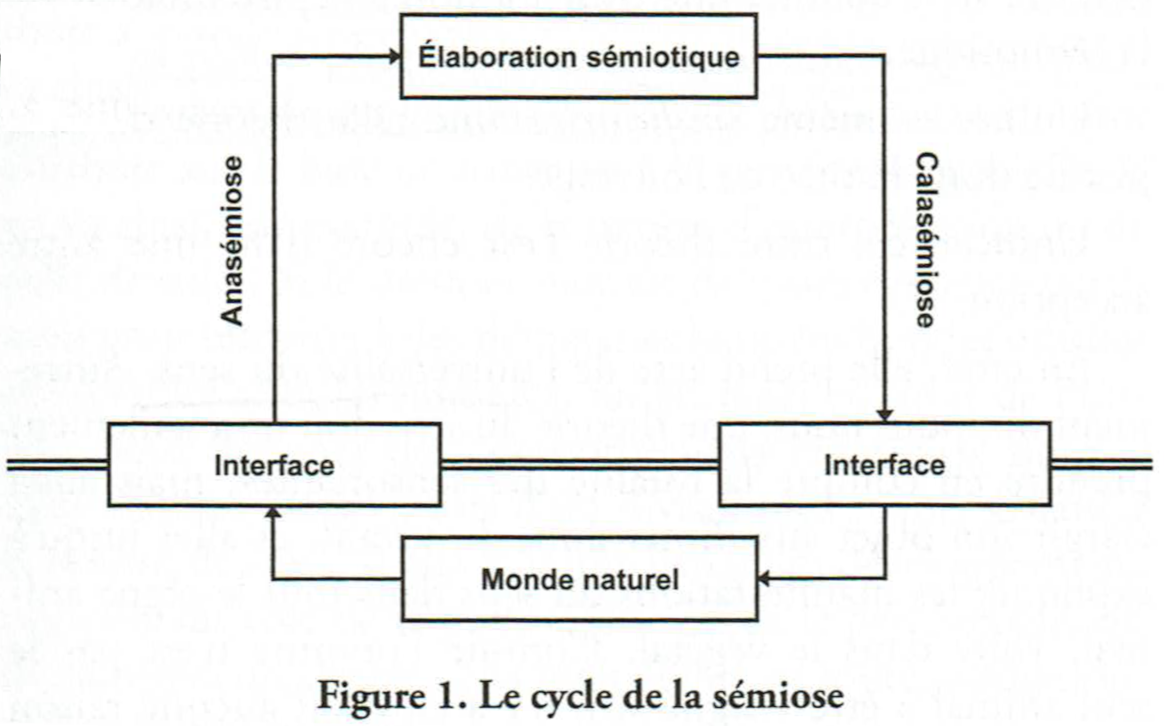
\includegraphics[width=9.855cm,height=6.145cm]{media/100000010000048C000002D6F38927B016A358A1.png}

}

\caption{\label{fig-cyclesemiose}Cycle de la sémiose (µ et al., 2015a,
p. 10)}

\end{figure}%

Le second principe se base sur les travaux de (Hofstadter \& Sander,
2013) pour qui l'analogie est le «~moteur~» qui relie le discernement et
l'action en gardant le souvenir de cette relation qui devient à force de
répétition, une manière d'être en prenant chez Deleuze la forme d'un
«~pli~» qui est notre troisième principe ~:

\begin{quote}
«~L'opération de la perception constitue les plis dans l'âme, les plis
dont la monade est tapissée du dedans ; mais ceux-ci ressemblent à une
matière, qui doit dès lors s'organiser en replis extérieurs.~» (G.
Deleuze, 1988, p. 131)
\end{quote}

A la manière de deux miroirs qui plient la lumière en se reflétant l'un
dans l'autre à l'infini, discernement et action se réfléchissent en
pliant les flux d'information. Chaque pli décompose l'information en
signes dont les signifiés plongent vers l'intériorité en stimulant
l'intuition et dont les signifiants émergent vers des physicalités en
stimulant l'expression.

Entre discerner et agir, intuition et expression, c'est dans ce
«~milieu~» qu'Augustin Berque décrit une «~pulsation existentielle~» mue
par la «~raison trajective~» que nous prenons comme quatrième principe :

\begin{quote}
«~la raison trajective, elle est en effet dans la pulsation
existentielle qui, par la technique, déploie notre corps en monde sur la
terre, et qui simultanément, par le symbole, reploie le monde en notre
chair ~»~ (Berque, 2009a, p. 402)
\end{quote}

Cette raison pilote la réflexion en modifiant l'inclinaison du pli vers
le discernement de signifiés ou vers l'expression de signifiants. Elle
procède de processus que nous contrôlons consciemment et d'autres plus
imprévisibles et incontrôlables qui se produisent en fonction d'une
multitudes de pliages et de leurs capacités à ce faire, ce défaire, ce
bloquer suivant un cinquième principe celui du degrés de flexibilité
(Clément, 2021).

Les cycles de sémioses, les analogies, les plis, les pulsations
existentielles, les degrés de flexibilité structurent et produisent nos
connaissances tout au long de nos vies en développant trois pouvoirs
fondamentaux~: discerner, raisonner, agir. Notre hypothèse principale
est qu'il est possible de cartographier ces connaissances en
représentant les pliages et leurs dynamismes dans trois directions~:
vers l'intériorité (discerner), en boucles récursives (raisonner) et
vers l'extérieur (agir). À chaque pulsation existentielle, à chaque
événement de nos vies, à chaque pli, ces pouvoirs augmentent ou
diminuent accentuant ainsi des rapports privilégiés, d'autres, plus
secrets, et même certains qui nous restent inconnus. De ce point de vue,
nous n'adoptons pas la conjecture au cœur des recherches en IA depuis
1955, formulée à l'occasion de séminaire d'été à Dartmouth par John
McCarthy, Marvin Minksy, Claude Shannon et Nathaniel Rochester
(Leveau-Vallier, 2023, p. 39) qui prend comme principe que tous les
aspects de l'intelligence peuvent être décrits avec une précision telle
qu'une machine peut les simuler.

Ainsi, la pulsation varie continuellement, elle est parfois instantanée
par exemple quand on rit, elle peut aussi prendre beaucoup de temps
quand un souvenir longtemps oublié émerge petit à petit~; elle devient
un métier quand à force de pratiquer un geste particulier, celui-ci
s'automatise. Ces pulsations se transforment parfois en bêtises ou en
inconscience quand le pouvoir d'agir prend le pas sur les pouvoirs de
discerner et de choisir en occultant leurs pliages potentiels. Suivant
leurs fréquences, les pulsations existentielles forment des ondes dont
la vitesse de propagation est fonction de leur longueur (distance
séparant deux maxima consécutifs de l'amplitude entre physicalités et
intériorité) et du milieu dans lequel elles se déploient. La
catégorisation et l'analyse de ces ondes renvoient globalement à une
réflexion sur la modélisation de l'esprit qui dépasse le cadre de ce
propos mais que nous illustration par le diagramme suivant :

\begin{figure}

\centering{

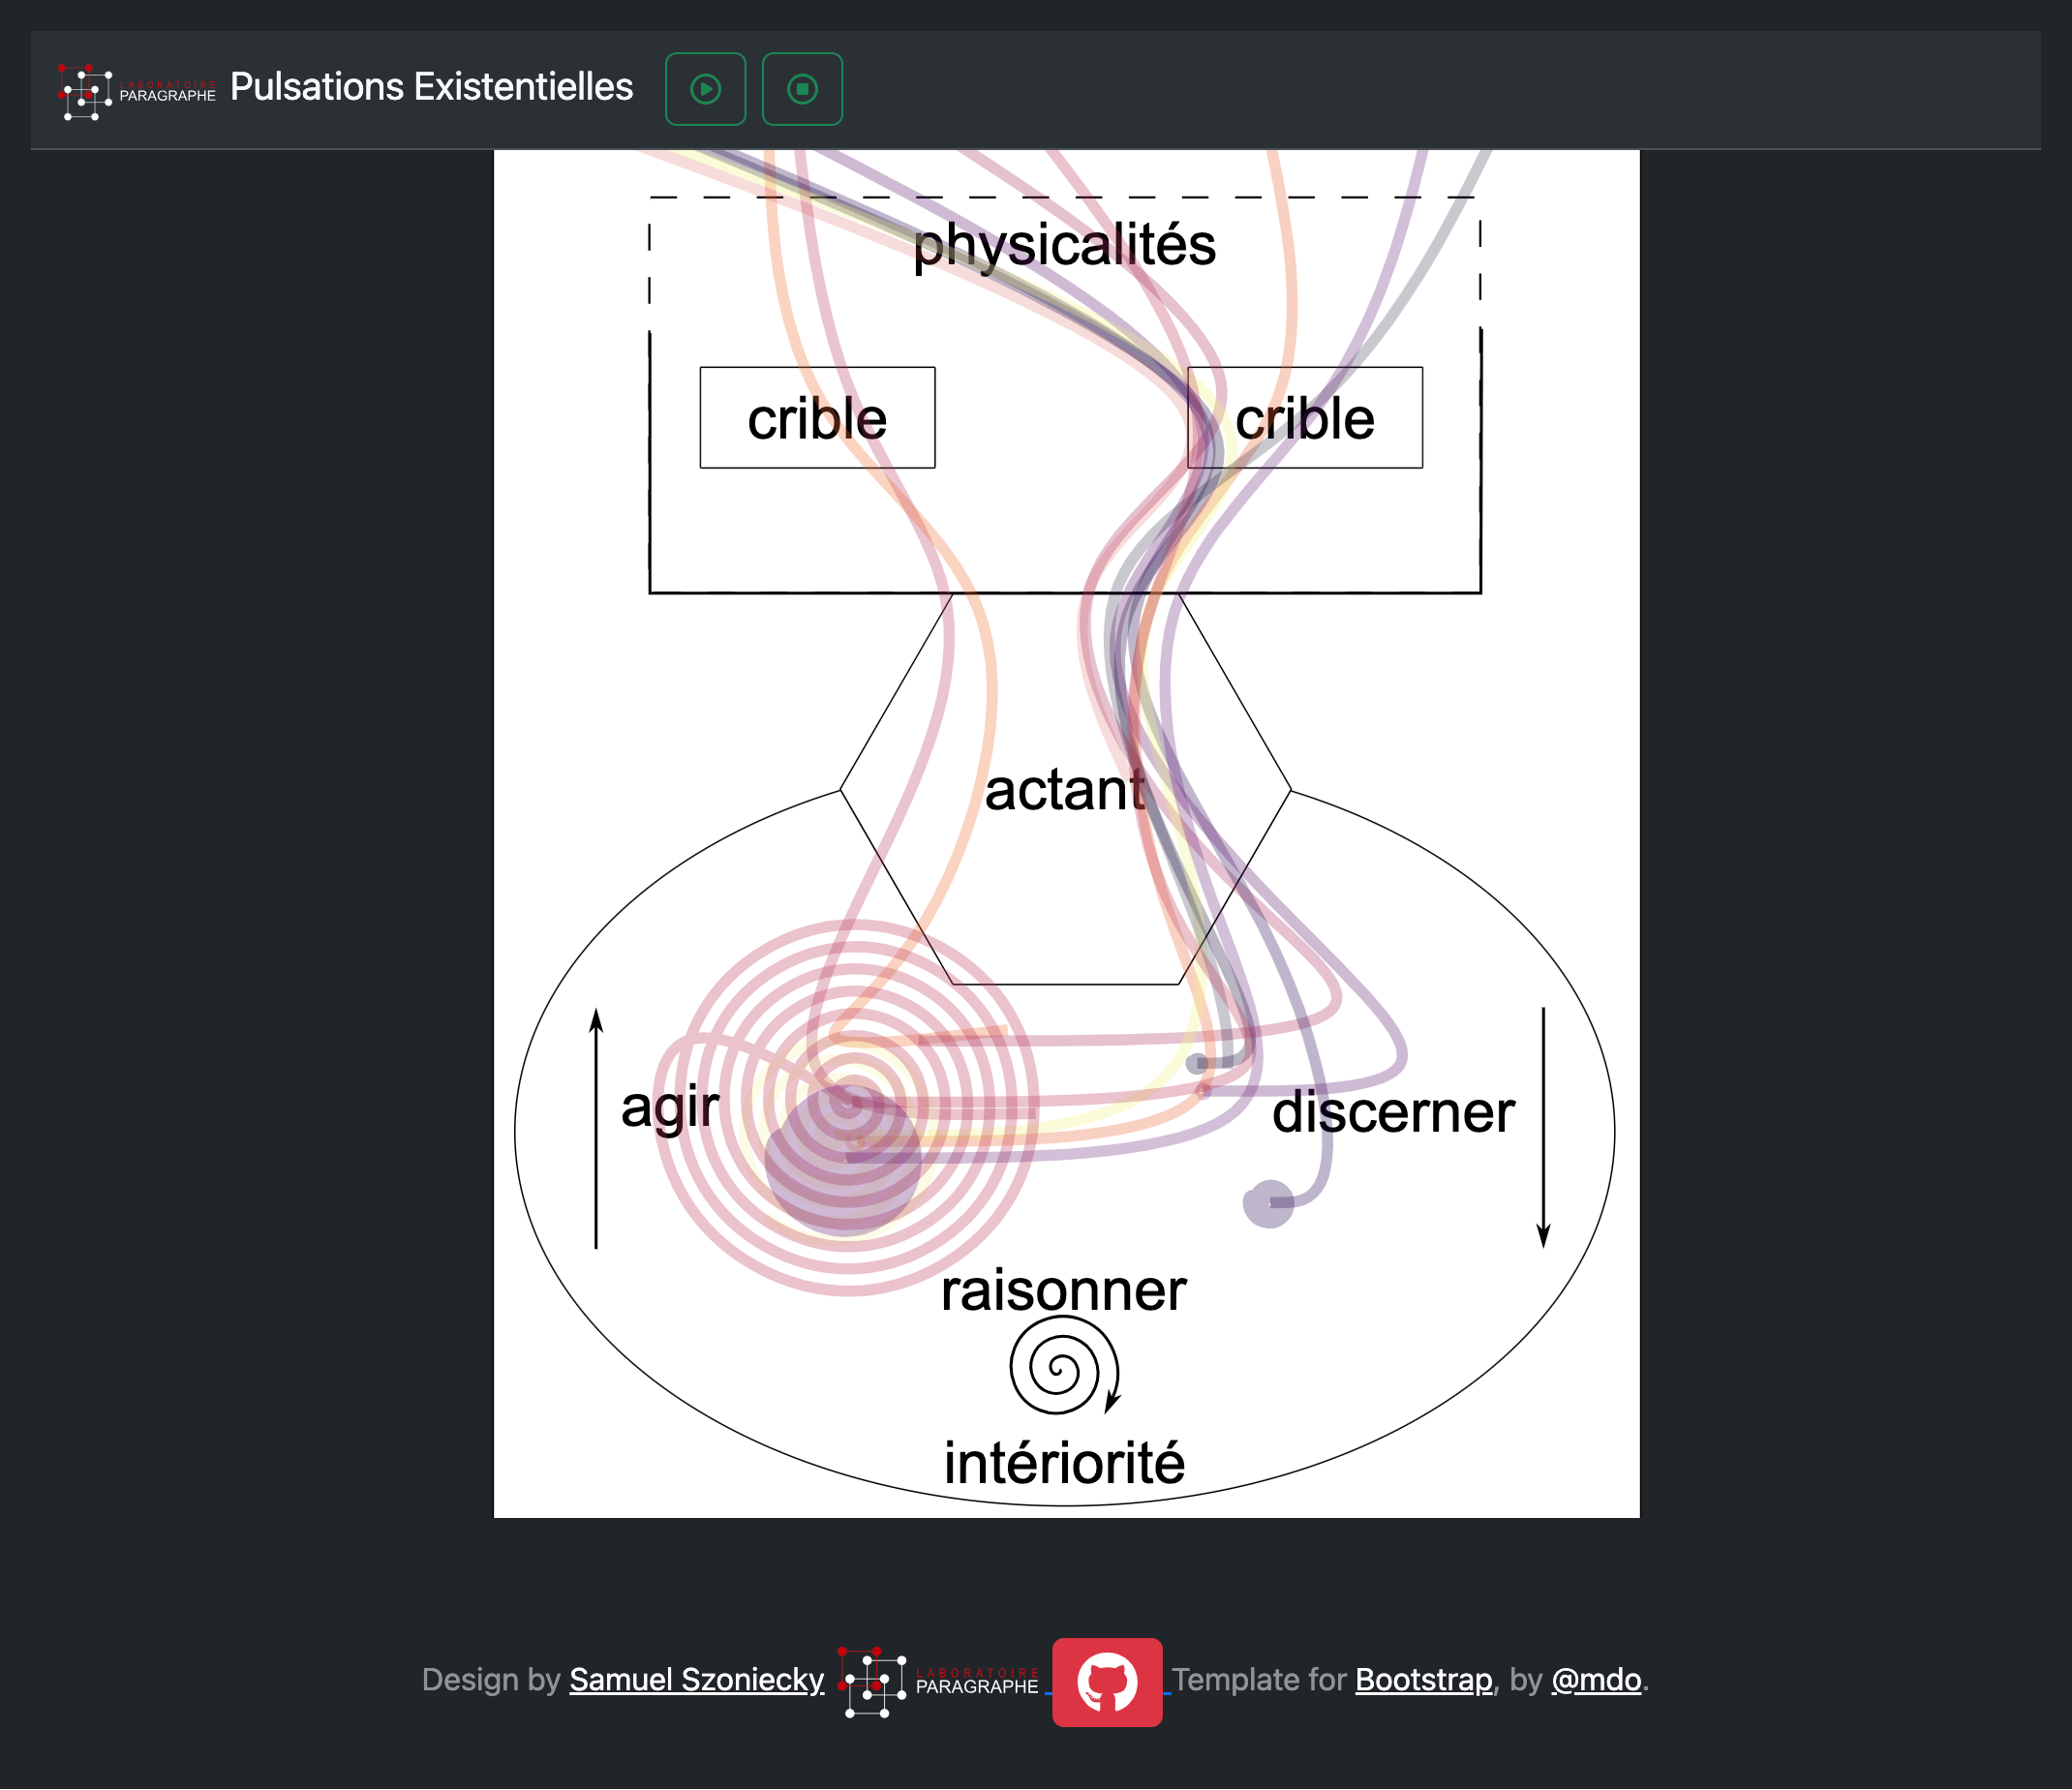
\includegraphics{images/localhost_samszo_HDR_pulsationsExistentielles.html.png}

}

\caption{\label{fig-dynamiquesPulsationsExistentielles}Dynamiques
pulsations existentielles}

\end{figure}%

Les chapitres suivants explicitent comment à partir de ces cinq
principes et de cette hypothèse principale, nous cartographions dans le
Web Section~\ref{sec-cartoEnvWeb} des connaissances qui se développent
dans l'espace et le temps Section~\ref{sec-repSpatioTempo} suivant les
pulsations existentielles d'un actant Section~\ref{sec-espaceActant}
entre des espaces matériels Section~\ref{sec-espaceMateriels} et
conceptuels Section~\ref{sec-espaceConceptuels}. Ces propositions sont
le résultat d'un travail de recherche d'une dizaine d'années que nous
présentons en détails dans \textbf{?@sec-part-modeliserConnaissances}.

\section{Cartographier dans un environnement Web}\label{sec-cartoEnvWeb}

Un environnement Web se base avant tout sur une architecture Client /
Serveur qui utilise le protocole HTTP pour organiser les échanges de
données entre des machines et des utilisateurs via un navigateur (Balpe,
Saleh, \& Lelu, 1996) cf.~ci-dessous\footnote{\begin{quote}
  cf.~\url{https://samszo.univ-paris8.fr/conf_errance/cours_systeme-information-programation-internet/slide.html?diapo=5}
  \end{quote}}.

\begin{figure}

\centering{

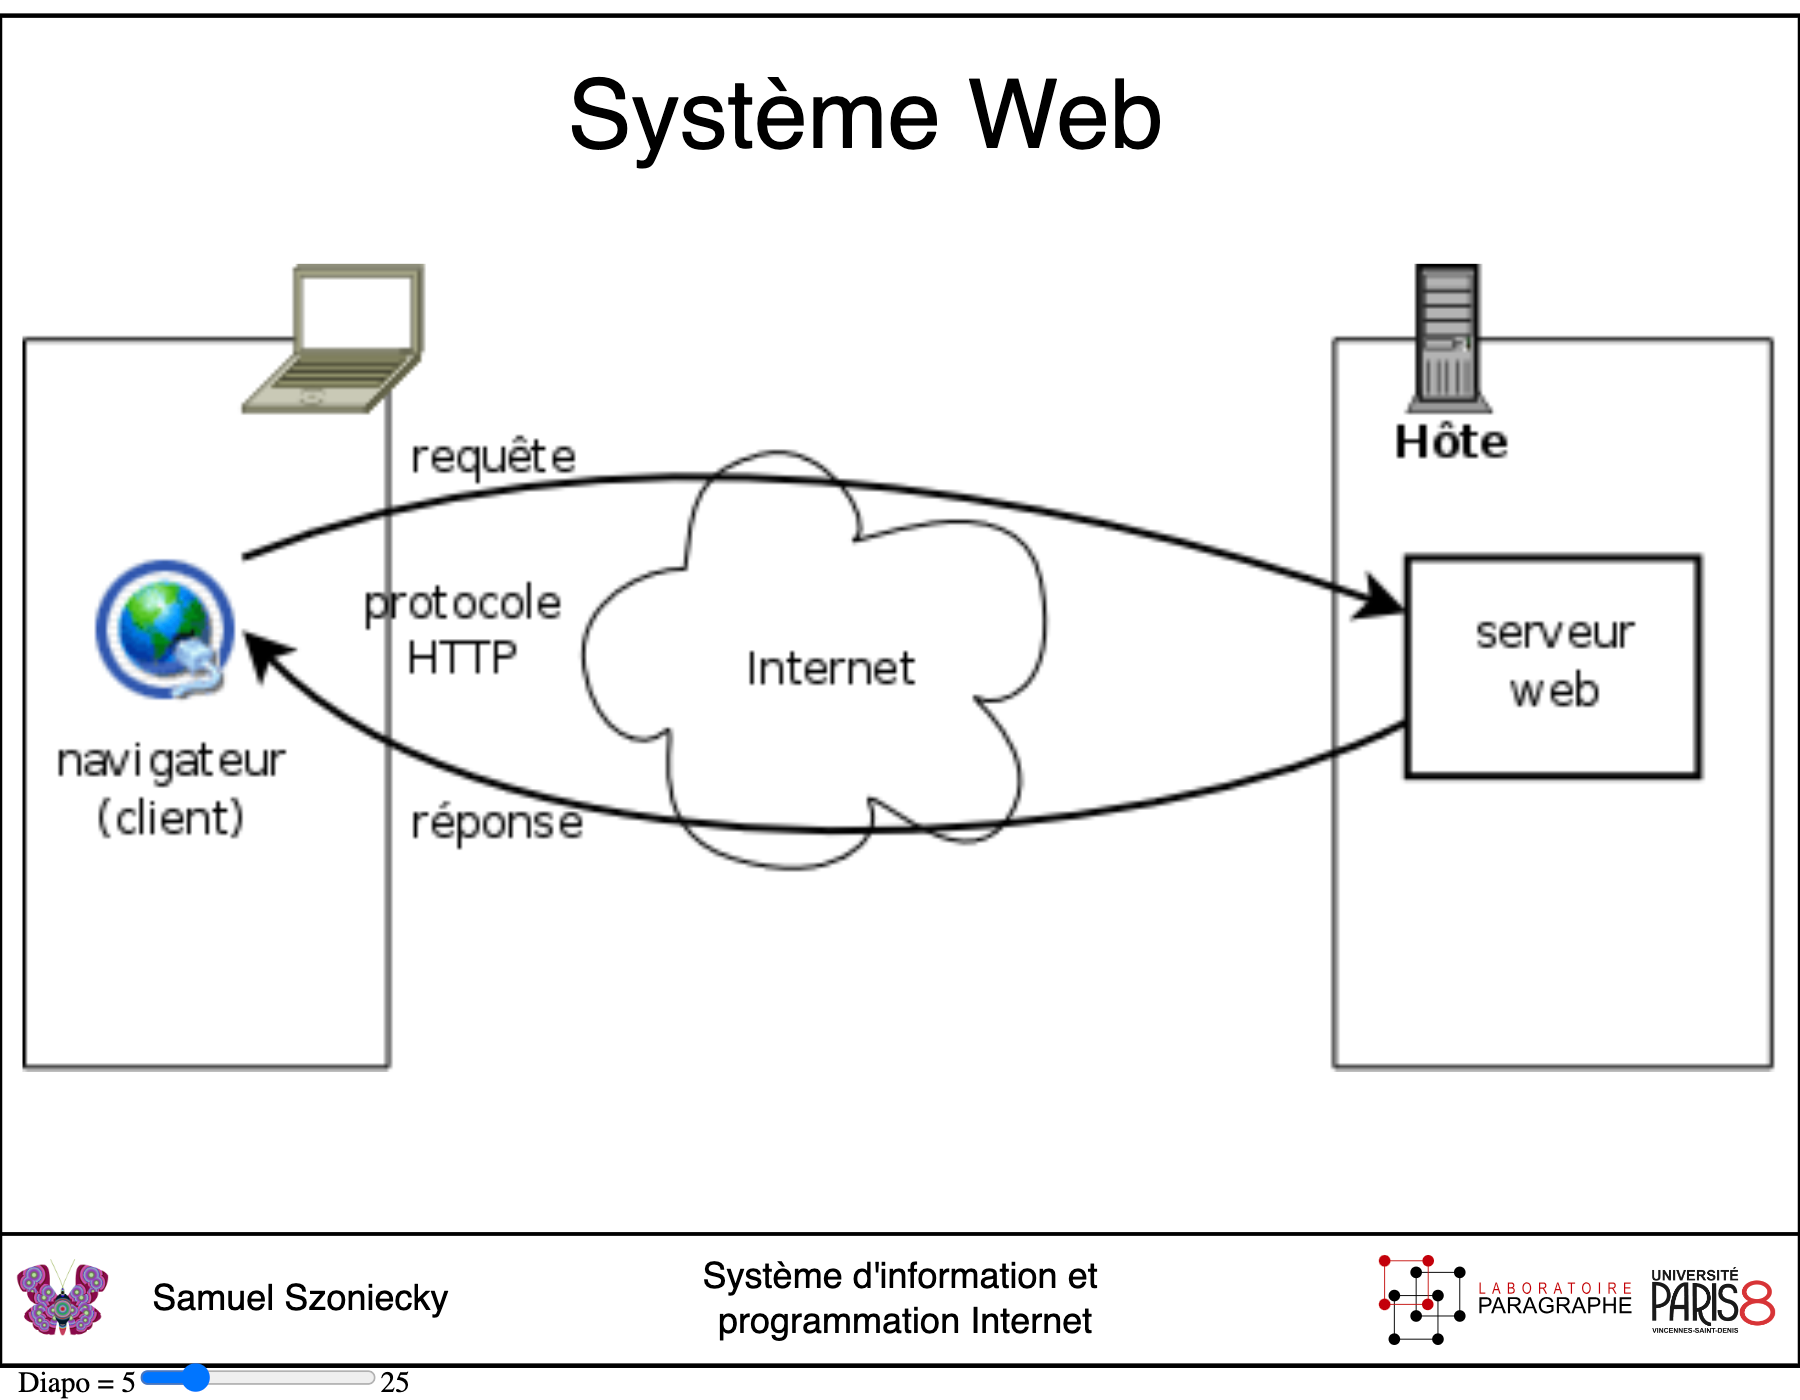
\includegraphics[width=8.269cm,height=6.253cm]{media/1000000100000708000005788D09F0CE68E86891.png}

}

\caption{\label{fig-ArchitectureClientServeur}Architecture Client /
Serveur}

\end{figure}%

Nous ne ferons pas ici une analyse des technologiques de représentation
des données (Andry, Kieffer, \& Lambotte, 2022; Fekete \& Boy, 2015)
préférant nous focaliser sur les outils et les méthodes que nous
utilisons dans le cadre de ce travail pour cartographier nos
connaissances. Nous ne détaillerons pas non plus tous les éléments qui
composent notre environnement\footnote{\begin{quote}
  disponibles sur notre forge logicielle~:
  \url{https://github.com/samszo}
  \end{quote}} mais uniquement les plus pertinents pour comprendre les
principes de cartographie que nous avons mis en place dans ce travail
pour gérer les données du coté serveur et naviguer dans leurs
représentations du coté client.

\subsection{Gérer les données sur les
serveurs}\label{sec-gestDonneesServeurs}

Les serveurs sont des machines qui fournissent des ressources via une
requête spécifique sur une adresse unique dans un environnement Web. Le
protocole HTTP définie les conditions d'adressage de ces requêtes et les
éventuels paramètres qui lui sont associés. Il existe une multitude de
solutions pour gérer les données à partir de ce protocole et des
langages informatiques associés comme PHP, Python, Java\ldots{} Pour nos
travaux de recherche, nous avions fait le choix de développer sur nos
serveurs, une boite à outils basée sur PHP et une base de données
spécifique (Szoniecky \& BouhaÏ, 2017, p. 141). Pour des questions de
maintenance de l'environnement, de facilités de développement et de
diffusion des données de la recherche, nous avons abandonné cette
solution pour utiliser depuis quelques années l'environnement Web
proposé par le CMS Omeka S\footnote{\begin{quote}
  \url{https://omeka.org/s/}
  \end{quote}}. Cette solution de gestion des archives numériques
offrent les fonctionnalités nécessaires pour modéliser une base de
données spécifique respectant les principes du Linked Open
Data\footnote{\begin{quote}
  \url{https://www.w3.org/egov/wiki/Linked_Open_Data}
  \end{quote}} et les moyens de manipuler ces données avec des
vocabulaires, des modèles de ressource, des modules et des thèmes
spécifiques. Une fois maîtrisé les éléments de cet environnement, les
données produites par les recherches deviennent accessibles,
manipulables et interopérables\footnote{\begin{quote}
  Lien vers l'API Omeka S des données de ce travail~:
  \url{https://samszo.univ-paris8.fr/omk/api}
  \end{quote}}.

\begin{quote}
«~En utilisant aujourd'hui un tableur ou une base de données ad hoc pour
stocker les données, non seulement on se prive de toute la richesse
sémantique des LOD et de leur potentiel de traitement, mais encore on
risque de ne pas pouvoir réutiliser l'information collectée. La
communauté de recherche va ainsi continuer à parcourir mille fois le
premier kilomètre, alors qu'une démarche collaborative de collecte de
l'information, soutenue par des plateformes de recherche fondées sur les
technologies sémantiques, permet de parcourir ensemble des milliers de
kilomètres et de disposer, en très peu de temps et en faisant levier sur
une curation collective des données, d'un graphe d'information de grande
complexité, qualité et richesse.~» (Beretta, 2023, sec. 15)
\end{quote}

Pour chaque projets de recherche et d'enseignement qui nécessitent de
manipuler des données, nous avons développé des environnements Omeka S
avec le cas échéant des modules et des thèmes spécifiques
Section~\ref{sec-pratiquesOmk}. Plus particulièrement, pour ce travail
d'HDR, nous avons rassemblé dans un environnement Omeka S les
informations concernant notre curriculum vitae et la veille
informationnelle que nous menons depuis plus de quinze ans
Section~\ref{sec-processusVeille}.

Pour ce faire, nous avons créé~:

\begin{itemize}
\item
  2 vocabulaires spécifiques~:

  \begin{itemize}
  \tightlist
  \item
    Jardin des connaissances~: nous utilisons ce vocabulaire pour gérer
    la modélisation des existences informationnelles dans un écosystème
    de connaissances\footnote{\begin{quote}
      le vocubulaire au format rdf turtle :
      \url{https://raw.githubusercontent.com/samszo/Omeka-S-module-JDC/master/data/vocabularies/jdc.ttl}
      \end{quote}}
  \item
    Formation Université Paris 8~: ce vocabulaire permet de modéliser
    l'architecture des enseignements dans l'enseignement
    supérieur\footnote{\begin{quote}
      le vocubulaire au format rdf turtle :
      \url{https://raw.githubusercontent.com/samszo/Omeka-S-module-JDC/master/data/vocabularies/fup8.ttl}
      \end{quote}}
  \end{itemize}
\item
  30 modèles de ressource\footnote{\begin{quote}
    la liste exhaustive est ici :
    \url{https://samszo.univ-paris8.fr/omk/api/resource_templates}
    \end{quote}} pour décrire les objets de recherche par exemple~:

  \begin{itemize}
  \tightlist
  \item
    Évènement CV~: utilisé pour décrire les événements d'un curriculum
    vitae
  \item
    JDC Actant~: utilisé pour décrire un actant dans un écosystème de
    connaissances
  \end{itemize}
\item
  4 modules spécifiques pour une gestion spécifique des données dans
  Omeka S:

  \begin{itemize}
  \tightlist
  \item
    Diigo Import : ce module permet d'importer les signets enregistrés
    dans une base de données Diigo y compris les copies
    d'écrans\footnote{\begin{quote}
      Dépôt du projet :
      \url{https://github.com/samszo/Omeka-S-module-DiigoImport}
      \end{quote}}.
  \item
    Zotero Import Plus~: ce module\footnote{\begin{quote}
      Dépôt du projet : \url{https://github.com/samszo/ZoteroImportPlus}
      \end{quote}} basé augmente le module Zotero Import pour importer
    les notes prises dans Zotero ainsi que les documents associés aux
    références bibliographiques.
  \item
    JDC~: ce module\footnote{\begin{quote}
      Dépôt du projet :
      \url{https://github.com/samszo/Omeka-S-module-JDC}
      \end{quote}} fourni les interfaces nécessaires pour modéliser un
    écosystème de connaissances suivant une ontologie éthique
    Section~\ref{sec-modeleOntoEthique}.
  \item
    CartoAffect~: ce module\footnote{\begin{quote}
      Dépôt du projet :
      \url{https://github.com/samszo/Omeka-S-module-CartoAffect}
      \end{quote}} permet de gérer les données pour la modélisation et
    la présentation des affects en relation avec un écosystème de
    connaissances.
  \end{itemize}
\end{itemize}

\subsection{Naviguer dans les
représentations}\label{sec-naviguerRepresentations}

La consultations de notre écosystème de connaissances se fait avec un
navigateur Web comme Chrome ou Firefox et passe par des représentations
que les utilisateurs explorent suivant les principes hypertextuels. Ces
représentations consistent à mettre en relation des données avec un
système de coordonnées cartésiennes qui possèdent 2 dimensions (
Figure~\ref{fig-coor2D}) ou 3 dimensions (Figure~\ref{fig-coor2D} ) .
Ces coordonnées définissent des points qui sont associés pour former des
lignes et des plans et ainsi disposer d'un vocabulaire graphique
élémentaire (Kandinsky, 1991). Toutefois, la réalisation de cartographie
en 3 dimensions demande beaucoup de temps et des compétences dont nous
ne disposons pas dans le contexte de ce travail
(\textbf{?@sec-pulsaExi3D}). Pour les graphiques que nous présenterons,
nous avons donc décidé de n'utiliser que le système de coordonnées
planaires. Il nous faut donc définir comment utiliser les 2 dimensions
(x, y) pour représenter les multiples propriétés de nos données. On peut
envisager de nombreuses solutions mais toutes ne seront pas
compréhensibles ni facilement manipulables suivant les données et les
échelles auxquelles on souhaite les représenter. Nous choisissons donc
de multiplier les environnements graphiques en deux dimensions et de les
interconnecter les uns avec les autres afin de former un écosystème
graphique présentant de manière optimale les multiples propriétés que
les données possèdent.

\begin{figure}

\centering{

\href{https://commons.wikimedia.org/wiki/File:Rovinna_kartezska_soustava_souradnic.svg}{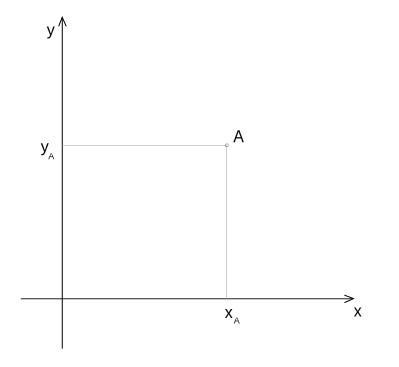
\includegraphics{index_files/mediabag/media/100019CC000029720000261A8EDA4DB42B40D384.pdf}}

}

\caption{\label{fig-coor2D}Coordonnées cartésiennes : planaires}

\end{figure}%

\begin{figure}

\centering{

\href{https://commons.wikimedia.org/wiki/File:Rectangular_coordinates.svg}{\includegraphics{index_files/mediabag/media/10003C4200002F5F00002EF5D54C4825D5249FE4.pdf}}

}

\caption{\label{fig-coor3D}Coordonnées cartésiennes :
tridimensionnelles}

\end{figure}%

Dans ce contexte d'écosystème graphique (Aït-Touati et al., 2019; Zreik,
2010), il est très important de disposer des moyens pour créer des
graphiques à partir des données mais aussi de manière réciproque gérer
les données à partir des graphiques en concevant des interactions riches
entre les données, les graphiques et leurs utilisateurs afin d'effectuer
les quatre actions fondamentales sur les données~: Cread Read Update
Delete (CRUD). Nous ne sommes pas dans une vision statique de la
représentation des données comme pouvait l'être (Bertin, 1999) qui
prenait comme principe que les graphiques devaient être imprimables. Ce
qui compte aujourd'hui c'est la capacité qu'ont les systèmes de
visualisation d'être manipulables pour créer les conditions d'une
interprétation des données (Drucker, Mignon, \& Bortolotti, 2020) et
l'expression d'une argumentation spécifique (Desfriches Doria \&
Meunier, 2021a).

C'est pourquoi nous avons choisi de travailler dans un environnement Web
afin de créer dynamiquement des graphiques à partir d'un flux de données
et surtout de rendre ces graphiques interactifs. L'autre choix important
que nous avons fait est d'utiliser le langage graphique SVG\footnote{\begin{quote}
  \url{https://developer.mozilla.org/en-US/docs/Web/SVG}
  \end{quote}} qui permet de manipuler chaque composant graphique de
manière autonome (Fry, 2008). Ainsi les points, les lignes et les plans
disposent d'une autonomie en terme de propriétés graphiques,
événementiels et informationnelles. Grâce à la librairie JavaScript
D3.js\footnote{\begin{quote}
  \url{https://observablehq.com/@d3/gallery?utm_source=d3js-org&utm_medium=hero&utm_campaign=try-observable\#maps}
  \end{quote}} (Data Driven Document) nous pouvons gérer ces propriétés
en pilotant les graphiques à partir des données ou à l'inverse les
données à partir des graphiques.

Dans cette environnement Web très ouvert et fertile, les possibilités de
dynamisme et d'interaction entre les données, les graphiques et leurs
utilisateurs sont potentiellement infinies. Il convient donc de
spécifier plus précisément les choix que nous avons fait pour
cartographier nos connaissances.

\section{Représentations spatio-temporelles}\label{sec-repSpatioTempo}

Les premières informations à prendre en compte dans la cartographie des
connaissances sont le temps et l'espace qui constituent une base
fondamental de la recherche en sciences humaines~: l'histoire et la
géographie. Ce sont les données communes à toutes les analyses en
sciences humaines ~: quand~? Où~?

\subsection{Cartographier la géographie}\label{sec-cartoGeo}

Pour réfléchir sur ces informations les humains ont depuis longtemps
développé des systèmes de représentations que ce soit pour le temps
(Domenget, Miège, \& Pélissier, 2017; Rosenberg \& Grafton, 2013),
l'espace (Béguin \& Pumain, 2017) ou la combinaisons des deux
(Aït-Touati et al., 2019; Giacona, Martin, Eckert, \& Desarthe, 2019; M.
Serres, 1997). Nous ne rentrerons pas ici dans l'analyse de ces
représentations cela dépasserais de loin notre propos qui est de
présenter nos principes cartographiques. Nous renvoyons le lecteur
curieux à la veille que nous faisons depuis plus de dix ans sur cette
question\footnote{\begin{quote}
  \url{https://www.diigo.com/user/luckysemiosis?query=\%23spatiotempo}
  \end{quote}}.

Sur notre Terre, les données spatiales sont définis par trois
propriétés~: une latitude, une longitude et une altitude. Les
représentations des données géographiques sont aujourd'hui grandement
aidées par les outils qui rendent disponibles pour les concepteurs les
fonctionnalités nécessaires à la manipulation des cartes. Le principe de
représentation est commun à tous ces outils~: x = longitude, y =
latitude. Ce qui diffère c'est le type de projection utilisé pour
représenter les données suivant un point de vue particulier qui mettra
l'accent sur une dimension spatiale. Les exemples ci-dessous montrent
comment suivant le type de projection les représentations se
transforment~:

\begin{longtable}[]{@{}
  >{\raggedright\arraybackslash}p{(\columnwidth - 4\tabcolsep) * \real{0.3319}}
  >{\raggedright\arraybackslash}p{(\columnwidth - 4\tabcolsep) * \real{0.3319}}
  >{\raggedright\arraybackslash}p{(\columnwidth - 4\tabcolsep) * \real{0.3362}}@{}}
\caption[Exemples de projections géographiques]{Exemples de projections
géographiques\footnote{\begin{quote}
  \url{https://github.com/d3/d3-geo-projection}
  \end{quote}}}\label{tbl-projGeo}\tabularnewline
\toprule\noalign{}
\endfirsthead
\endhead
\bottomrule\noalign{}
\endlastfoot
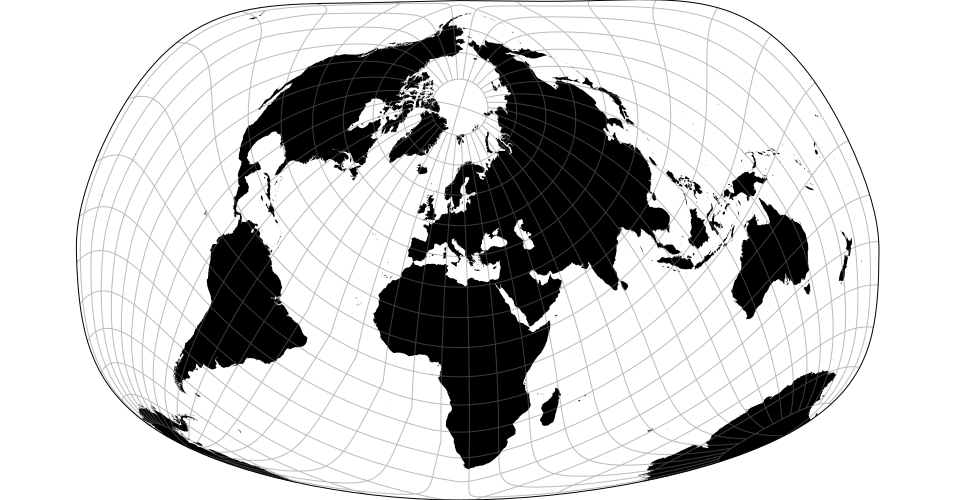
\includegraphics{media/10000000000003C0000001F4F33DE5F8AECF42B5.png} &
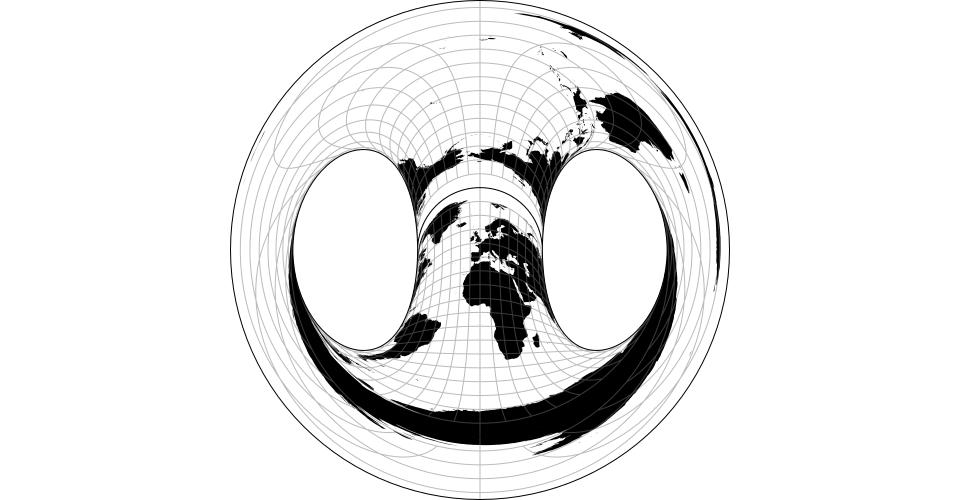
\includegraphics{media/10000000000003C0000001F46900D5D2AB4D8E23.png} &
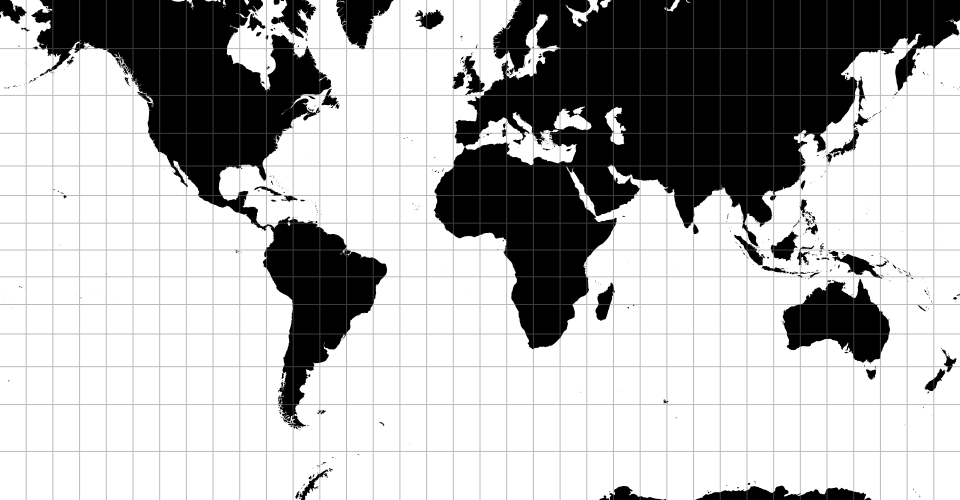
\includegraphics{media/10000000000003C0000001F47F8100241BAEED66.png} \\
Jacques Bertin's 1953 & Hammer retroazimuthal & Spherical Mercator \\
\end{longtable}

Dans notre cas, pour concevoir des cartes géographique en deux
dimensions nous utilisons des librairies JavaScript Open Source comme
leaflet.js\footnote{\begin{quote}
  \url{https://leafletjs.com/}
  \end{quote}} ou D3.js qui permettent de manipuler des données
géographiques modéliser avec le format GeoJSON\footnote{\begin{quote}
  \url{https://fr.wikipedia.org/wiki/GeoJSON}
  \end{quote}}. Voici par exemple la représentation géographique de mes
collaborations dans le monde à partir de mes dépôts dans HAL\footnote{\begin{quote}
  \url{https://samszo.github.io/StatsHAL/world.html?q=Samuel\%20Szoniecky}
  \end{quote}} \textbf{?@sec-datavizActiChercheur}~:

\begin{figure}

\centering{

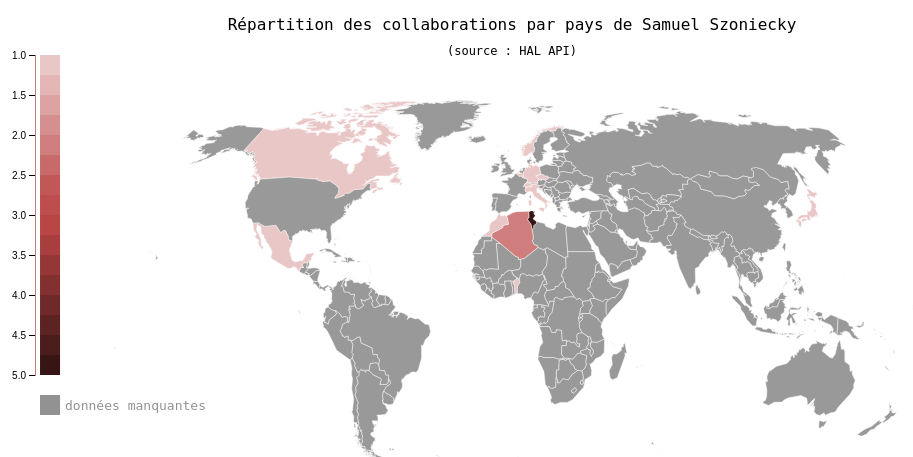
\includegraphics{media/1000000100000391000001C9A8374D4BE530A8B5.png}

}

\caption{\label{fig-collabMondeSamszo}Répartition des collaborations
dans le monde}

\end{figure}%

Cette carte montre les pays hors de la France où sont publiées mes
textes scientifiques et les conférences auxquelles j'ai participées.
Parallèlement aux données géographiques, la couleur des pays est
proportionnelle au nombre de collaborations. Cette carte montre que mes
collaborations se développent essentiellement avec des pays francophones
et des pays de l'hémisphère nord.

\subsection{Cartographier le temps}\label{sec-cartoTempo}

Pour les informations historiques, nous avons besoin de gérer deux
propriétés, une date de début et une date de fin. Notons que la durée
n'est pas une propriété nécessaire puisqu'elle se calcule à partir de la
différence entre la date de début et la date de fin. Nous posons comme
principe qu'une date de fin nulle indique une durée en cours. La frise
est sans doute la représentation la plus courante et la plus commode à
réaliser puisqu'elle associe une coordonnée graphique avec une échelle
de temps, le plus souvent x pour une représentation horizontal et
parfois y lorsqu'elle est verticale. Dans notre enfance, nous avons tous
réalisé des frises historiques, elles peuplent nos salles de classe et
prolifèrent sur le Web\footnote{\begin{quote}
  \url{https://bit.ly/3r9ROUa}
  \end{quote}}. Nous avons une compréhension évidente de la frise
historique, de son fonctionnement et des informations qu'elle diffuse~:
événements ponctuels, périodes. Voici par exemple la représentation en
frise historique de mon activité d'enseignant chercheur~:

\begin{figure}

\centering{

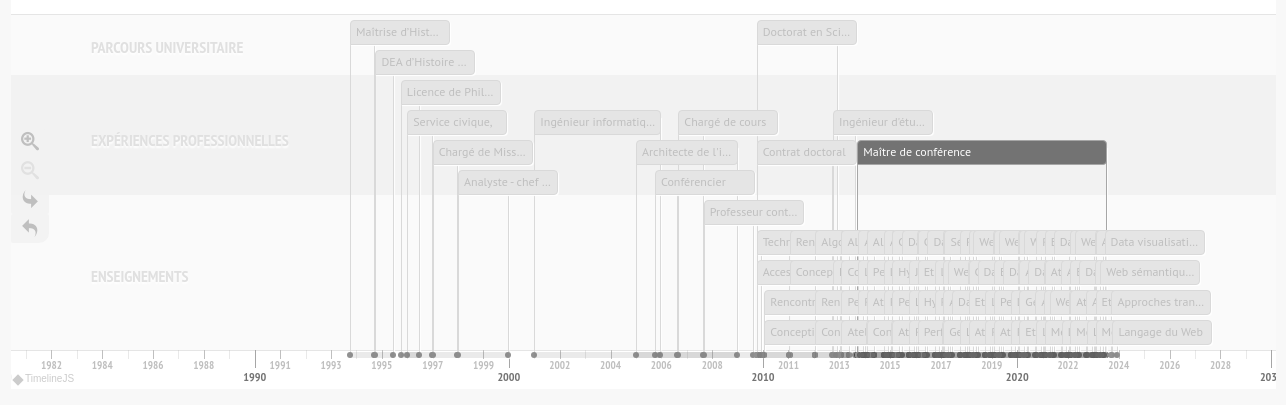
\includegraphics{media/10000001000005060000019591922F8EA1A9F073.png}

}

\caption{\label{fig-timelineCvSamszo}Timeline des activités d'enseignant
chercheur}

\end{figure}%

Cette frise historique\footnote{\begin{quote}
  Visualisation conçue à partir du modules Omeka S timeline
  (https://gitlab.com/Daniel-KM/Omeka-S-module-Timeline) que nous avons
  adapté à nos besoins.
  \end{quote}} montre l'évolution de mes activités d'enseignant
chercheur suivant plusieurs types d'activité. Comme les outils Web de
visualisation des cartes géographiques, cette visualisation fourni des
fonctions de zoom, de déplacement et d'hypertextualité pour faciliter la
lecture des données qui si elles sont trop détaillées, ne sont plus
visibles. Là encore, la cartographie des connaissances dans le Web est
conçu comme un outils de navigation dans les données.

Les connaissances sont toujours en rapport avec l'espace et le temps
mais nous posons comme hypothèse qu'entre les connaissances des
physicalités et celles des intériorités, entre l'étendu et la pensée,
l'espace et le temps n'ont pas les même modes de perceptions et
d'expressions.

\begin{quote}
«~La durée se dit en fonction des parties extensives et se mesure au
temps pendant lequel ces parties appartiennent à l'essence. Mais
l'essence en elle-même à une réalité ou une existence éternelle ; elle
n'a pas de durée, ni de temps qui marque l'achèvement de cette
durée.~»(G. Deleuze, 1968, p. 291)
\end{quote}

Nous suivons sur ce point les principes spinozistes d'une modélisation
ontologique corrélée à une éthique en définissant trois dimensions de
l'existence corrélées avec trois genres de connaissance\footnote{\begin{quote}
  \url{https://spinoza.fr/les-genres-de-connaissance-extrait-du-cours-de-gilles-deleuze/}
  \end{quote}} Section~\ref{sec-modeleOntoEthique}. Examinons maintenant
comment nous définissons de nouveaux principes cartographiques à partir
de ces propositions.

\section{Espaces matériels~: connaissances des
chocs}\label{sec-espaceMateriels}

A l'instar de (Bautier, 2016) nous pensons nécessaire «~de prendre en
compte la matérialité de la culture numérique~». Les technologies
numériques véhiculent sans doute des idées de dématérialisation à
travers des expériences de téléprésence, de virtualisation des échanges
et d'autonomisation de la forme logique par rapport à la base
matérielle. Mais peut-on encore parler de matière quand le contact avec
l'événement se fait à travers des écrans, des réseaux, des milliers de
kilomètres, des années, des algorithmes~?

Quoi qu'il en soit de cette «~dématérialisation~», nos connaissances
numériques passent nécessairement par une dimension matérielle car nous
sommes nous même constitué de matière~:

\begin{quote}
«~La sémiose, loin d'être un phénomène sans lien avec le corps, tire son
origine de celui-ci. Ce premier aspect de la corporéité du sens peut
être qualifié de cognitif : le signe émerge de l'expérience, et ne
saurait être étudié qu'à travers les interactions qu'il a avec son
contexte~» (µ, Édeline, \& Klinkenberg, 2016, p. 2)
\end{quote}

Les illusions que le numérique procure, tendent pour beaucoup à nous
faire croire à la dématérialisation en simulant par exemple des univers
immersifs où nous vivons d'autres actualités que celles de notre corps
avec des avatars de toutes sortes (Amato \& Perény, 2013). Mais en
dernière instance nous sommes matière et nous évoluons dans des espaces
matériels. Sur ce point nous nous opposons au spiritualistes qui
affirment «~qu'il existe une substance spirituelle (l'âme ou l'esprit),
indépendante de la matière, et qui serait, en l'homme, principe de vie
ou d'action.~» (Comte-Sponville, 1998, sec. 12).

Les interprétations par Deleuze de L'Étique de Spinoza décrive ces
espaces matériels comme étant la première dimension de l'existence celle
des «~parties extensives~»~:

\begin{quote}
«~Ces parties (corpora simplissima) {[}\ldots{]} se définissent
uniquement par leur déterminisme extérieur, et vont toujours par
infinités ; {[}\ldots{]} elles constituent la matière modale infiniment
variée de l'existence.'' (G. Deleuze, 2003, p. 110)
\end{quote}

Entre l'infiniment grand et l'infiniment petit (cf.~illustration ci
dessous) les parties extensives sont observables et modélisables à
toutes les échelles physiques de notre univers. Tout comme le choix
d'une projection géographique reflète un point de vue particulier, celui
des échelles de représentation contribue lui aussi à l'expression d'une
subjectivité spécifique.

\begin{figure}

\centering{

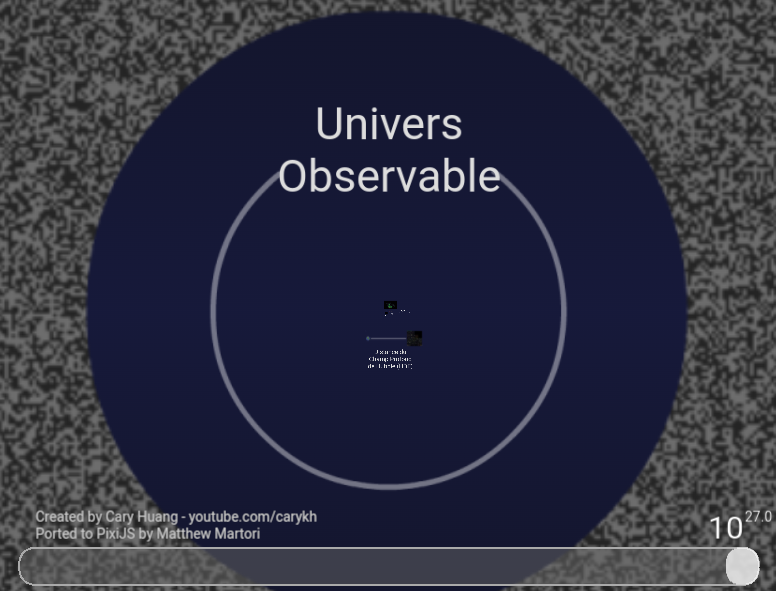
\includegraphics{media/10000001000003080000024F28EEAE4E22F24B62.png}

}

\caption{\label{fig-echelleUnivers}Échelle de l'univers - univers
observable https://htwins.net/scale2/}

\end{figure}%

\begin{figure}

\centering{

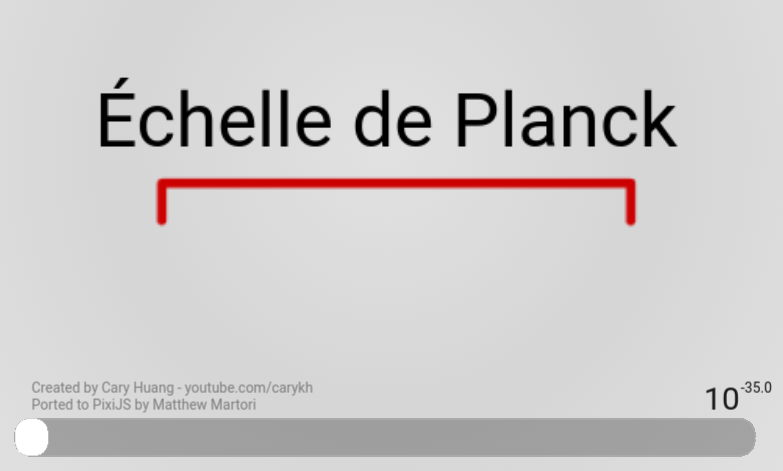
\includegraphics{media/100000010000030F000001D7889CE02FB9E347F3.png}

}

\caption{\label{fig-echelleUniversPlank}Échelle de l'univers - limite de
Plank https://htwins.net/scale2/}

\end{figure}%

Les parties extensives correspondent aux «~physicalités~» des milieux
que nous habitons, elles en sont l'indispensable matérialité. Cette
nécessité de la matière est corrélé à des connaissances, elles aussi
nécessaires, celles du premier genre de connaissance~: les idées
inadéquates~:

\begin{quote}
«~L'idée inadéquate, c'est l'idée inexpressive et non expliquée :
l'impression qui n'est pas encore expression, l'indication qui n'est pas
encore explication.~» (G. Deleuze, 1968, p. 136)
\end{quote}

Pour expliquer à quoi correspondent les connaissances du premier genre,
Deleuze décrit dans un de ces cours l'expérience d'une personne au bord
de la mer~:

\begin{quote}
«~Bien alors c'est quoi la connaissance du premier genre ? Eh bien
allez, j'y vais, je me lance, je suis dans le premier genre de
connaissance. Je me lance, je barbote, comme on dit. Qu'est-ce que ça
veut dire barboter ? Barboter c'est tout simple, ça indique bien, on
voit bien que c'est des rapports extrinsèques. Tantôt la vague me gifle,
et tantôt elle m'emporte. Ça c'est des effets de choc. C'est des effets
de choc, à savoir, je ne connais rien aux rapports qui se composent ou
qui se décomposent, je reçois les effets de parties extrinsèques. Les
parties qui m'appartiennent à moi, sont secouées, reçoivent un effet de
choc des parties qui appartiennent à la vague.~» (G. Deleuze, 1981)
\end{quote}

Donnons un autre exemple de ce premier genre de connaissance en vous
invitant à faire l'expérience des parties extensives suivantes~:

\begin{figure}

\centering{


\includegraphics{media/10000001000001EB0000002F6C14D0CF44FAB1C7.png}

}

\caption{\label{fig-partExt1}Parties extensives 1}

\end{figure}%

Sauf si vous connaissez le tamoul, le texte ci-dessous est pour vous
comme un choc, vous ne connaissez rien des rapports qui se composent ou
se décomposent, vous ne voyez que les parties extensives du texte. Pour
être plus précis, vous pouvez tout de même discerner des rapports
puisque vous savez que l'image est un texte composé de caractères qui
composent des mots séparés par des espaces. Par contre, vous n'avez
aucune idée des concepts présents dans le texte, vous avez connaissance
des signifiants mais pas des signifiés\footnote{\begin{quote}
  Précisons toutefois que l'humain est particulière efficace pour la
  paréidolie (\textbf{Dufort2015?}), ce qui lui permet de donner du sens
  à des formes ambiguës et donc de créer des signifiés quelles que
  soient les parties extensives qu'il discerne.
  \end{quote}}. D'une certaine manière vous êtes comme un OCR (optical
character recognition) capable de reconnaître des caractères et des mots
dans une image. Mais à l'inverse d'une machine numérique qui avant la
reconnaissance du texte décompose l'image en une multitude de points
ayant chacun leurs coordonnées cartésiennes et leurs propriétés de
couleur, vous commencez par reconnaître le texte puis vous le décomposez
en mots et en caractères. Cette différence entre la machine et l'humain
dans le processus de connaissances est au cœur d'une problématique
fondamentale de la gestion mécanique du sens~:

\begin{quote}
«~il y a un conflit entre l'holisme du sens et le mécanisme de la
syntaxe. Le sens d'un texte dépend de son contexte, le sens d'un
paragraphe dépend aussi du texte dans lequel il s'intègre, le sens d'un
mot du paragraphe qui le contient, etc. : le sens va du global au local,
de la compréhension globale vers l'analyse. Or, le formalisme opère de
manière inverse : le sens d'une formule logique se construit à partir du
sens de ses parties, allant du local au global.~» (B. Bachimont et al.,
2011, sec. 11)
\end{quote}

Ce conflit est d'autant plus flagrant quand le même texte est présenté
dans une écriture que vous connaissez (Figure~\ref{fig-partExt2}). Dans
ce cas, vous ne faites plus la décomposition du texte en parties
extensives le constituant mais vous accédez directement à sa
signification car vous avez appris à lire, c'est-à-dire à discerner les
compositions de rapports dans les parties extensives et vous accédez
ainsi à un autre genre de connaissance celui des signifiants.

\begin{figure}

\centering{

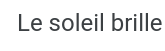
\includegraphics{media/10000001000000A500000033DA0B4C29741E4F62.png}

}

\caption{\label{fig-partExt2}Parties extensives 2}

\end{figure}%

Notre principe de cartographie des espaces matériels consiste à les
considérer uniquement en tant que physicalités composées de parties
extensives modélisables par leurs propriétés physico-chimique~: largeur,
hauteur, profondeur, masse, couleur, atome, molécule\ldots{} Par
exemple, dans les espaces matériels un livre est considéré du point de
vue de sa taille, son nombre de page, son poids, sa matière etc\ldots{}
Dans l'espace matériel, on ne prend pas en compte l'auteur ou la
thématique du livre qui respectivement seront cartographiés comme actant
(Section~\ref{sec-espaceActant}) et comme élément d'un espace conceptuel
(Section~\ref{sec-espaceConceptuels}). Dans les espaces matériels les
mots du livre sont des traces de couleur qui génère des connaissances de
l'ordre des chocs ; c'est à dire une réaction entre des parties
extensives celles de la trace et celles de nos capteurs biologiques ou
artificiels. Notons que ces chocs en entraînent d'autres qui eu mêmes se
propagent dans un phénomène d'accroissement de l'entropie constitutif de
l'univers chaotique du premier genre de connaissances, celui des idées
inadéquates qui se répandent sans fin par composition et décomposition~:

\begin{quote}
«~qu'est-ce que vous racontez là, mais alors cette nature, c'est un pur
chaos ! Pourquoi c'est un pur chaos ? Parce que vous remarquerez que,
chaque fois qu'un corps agit sur un autre, il y a toujours composition
et décomposition à la fois. Ce n'est pas à ce niveau-là que je pourrais
dire, il y a du bon et du mauvais. Pourquoi ? Parce qu'il y a forcément
composition et décomposition, les deux l'un dans l'autre.~» (G. Deleuze,
1981)
\end{quote}

Ces compositions et décompositions des corps les plus simples que sont
les parties extensives sont modélisables suivant une hiérarchie de
parties et de sous-parties. Par exemple le livre est décomposable en
parties plus petites~: page → paragraphe → phrase → mot → caractère. Ce
même livre est aussi composable avec d'autres parties plus vastes~:
étagère → salle → bibliothèque. La modélisation des espaces matériels
est une structure hiérarchiques qui potentiellement se compose jusqu'aux
limites de l'univers observable (Figure~\ref{fig-echelleUnivers}) et se
décompose jusqu'à l'infiniment petit de l'échelle de Plank
(Figure~\ref{fig-echelleUniversPlank}) en passant par l'échelle de
l'être humain (Figure~\ref{fig-echelleHumain}). Nous verrons plus loin
combien le choix de l'échelle cartographique est primordial
(\textbf{?@sec-illusionExhaustivite})

\begin{figure}

\centering{

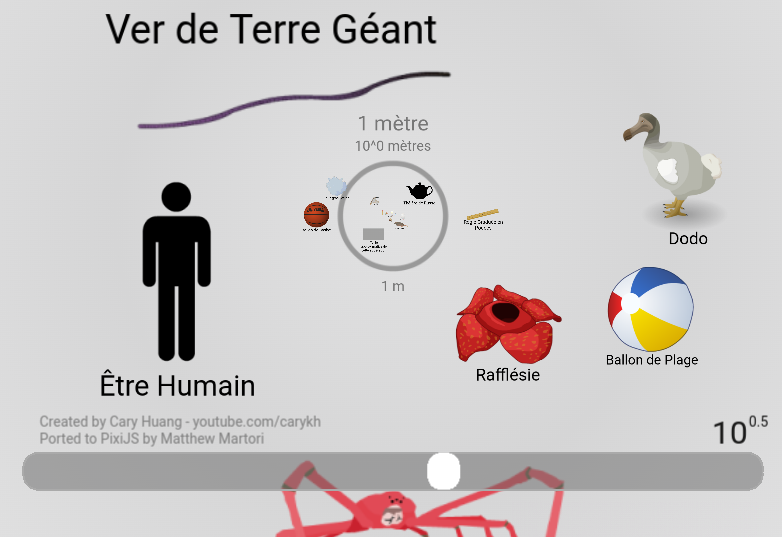
\includegraphics{media/100000010000030E00000219C3ED261C6D514C78.png}

}

\caption{\label{fig-echelleHumain}Échelle de l'univers - être humain}

\end{figure}%

Pour cartographier les espaces matériels en tant qu'ensemble des parties
extensives définissables par leurs propriétés physico-chimique et leurs
compositions vers l'infiniment grand et décompositions vers l'infiniment
petit, nous optons pour un modèle de diagramme hiérarchique appelé
«~treemap~» et proposé par (Shneiderman, 1998) qui se compose de
rectangles imbriqués représentant un élément et ses sous parties et dont
la taille des rectangles est proportionnelle à la valeur numérique d'une
propriété, par exemple le nombre d'éléments que contient la sous
partie~.

En utilisant l'objet TreeMap\footnote{\begin{quote}
  https://d3js.org/d3-hierarchy/treemap
  \end{quote}} de la librairie D3.js, nous avons implémenté ce modèle de
diagramme dans un module JavaScript (Section~\ref{sec-jdcPhysiques})
pour le rendre dynamique, interactif et ainsi représenter les espaces
matériels que nous cartographions soit à partir de données existantes
soit en les créant au fur et à mesure de l'exploration. Notons que pour
faciliter la visualisation des dimensions physiques complexes, nous
avons implémenté une navigation directe vers une partie ou une
sous-partie et une navigation hiérarchique par zoom dans une partie et
dé-zoom vers le parent. Par exemple, nous avons cartographié notre CV en
utilisant ce modèle de diagramme avec comme paramètre de taille des
rectangles la durée d'un événement~:

\begin{figure}

\centering{

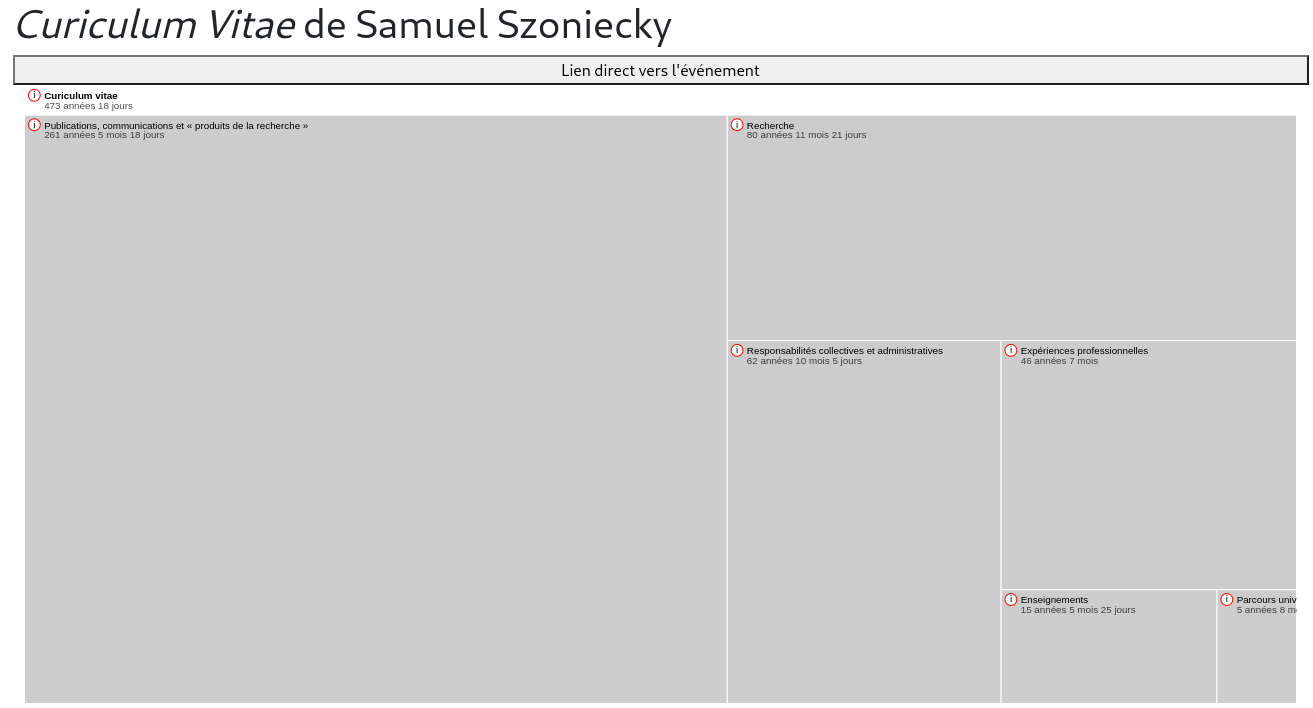
\includegraphics{media/1000000100000521000002C4F34D431EF036AFFE.png}

}

\caption{\label{fig-treeMapCv}Treemap d'un Curiculum Vitae}

\end{figure}%

Dans le cas de ce diagramme, la durée d'un événement cumule l'ensemble
des durées des événements qui le compose ce qui explique une durée de
plusieurs centaines d'année pour le CV. D'autre part, cette durée
exprime une période de travail et ne prend pas en compte les activités
parallèles à l'inverse de la frise historique
(Figure~\ref{fig-timelineCvSamszo}).

Dans les espaces matériels les connaissances sont des chocs qui ne dure
qu'un instant, celui du contact entre les parties extensives. On peut
les dater plus ou moins précisément, ils peuvent se répéter encore et
encore mais ils n'ont pas de durée. Ce qui dure c'est l'onde du choc qui
se propage dans les physicalités et dans les intériorités des acteurs
qui participent à l'événement ce qui génère d'autres chocs dans les
espaces matériels et des connaissances d'un autre genre dans les espaces
conceptuels.

\section{Espaces conceptuels~: connaissances des
essences}\label{sec-espaceConceptuels}

A l'opposé des espaces matériels-physiques et de la connaissance des
chocs, nos connaissances se composent aussi dans nos intériorités~:

\begin{quote}
«~Par le terme vague d' ``intériorité'', il faut entendre une gamme de
propriétés reconnues par tous les humains et recouvrant en partie ce que
nous appelons d'ordinaire l'esprit, l'âme ou la conscience -
intentionnalité, subjectivité, réflexivité, affect, aptitude à signifier
ou à rêver.~» (Philippe. Descola, 2005, p. 168)
\end{quote}

Comment cartographier ces espaces de connaissances ~? Comment mesurer
ces espaces~? Combien pèse une âme~?

\begin{figure}

\centering{

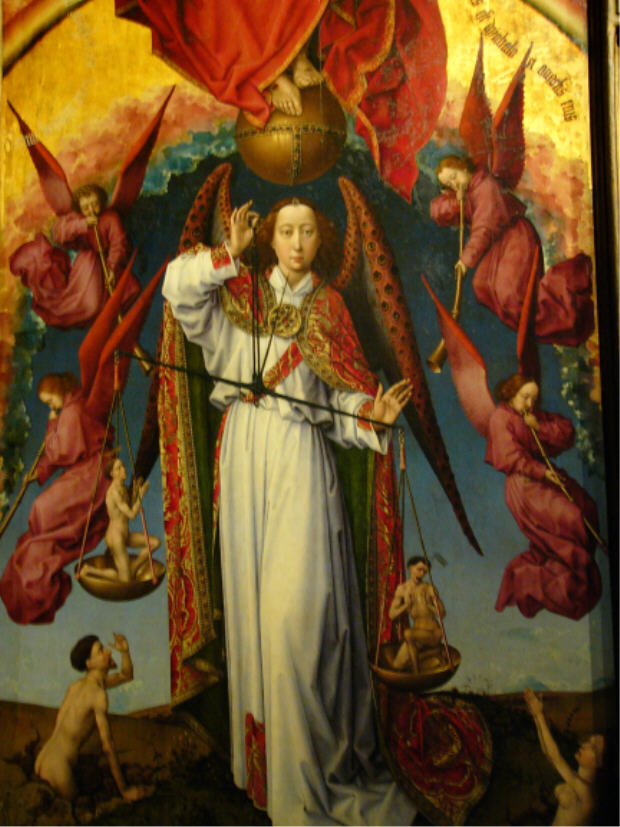
\includegraphics{media/100000000000026C0000033BDE0C2A2E5F4A6C07.jpg}

}

\caption{\label{fig-peseeAme}La pesée des âmes dans le retable
polyptyque du Jugement Dernier de Rogier van der Weyden aux Hospices de
Beaune, 1443-1452,
https://commons.wikimedia.org/w/index.php?curid=6028656}

\end{figure}%

La question du poids des âmes se pose depuis longtemps comme en témoigne
l'iconographie de la pesée des âmes. La psychostasie, nom donné à cette
activité de la pesée des âmes, touche historiquement les domaines de la
théologie, de la philosophie et de l'éthique mais intéresse aussi les
sciences de l'information et de la communication qui cherchent notamment
des réponses sur la mesure, l'analyse et la critique de ces espaces
informationnels immatériels qui ne sont pas mesurables de la même
manière qu'une planche de bois ou qu'une récolte de fruit car ils ne
sont pas soumis aux règles physiques de la matérialité tant qu'ils ne
sont pas exprimées. Dès le passage de ces espaces intérieurs vers une
forme d'expression quelle qu'elle soit (écrit, parole, clic sur un
bouton\ldots), ils se transforment en physicalités dont on pourra
mesurer les paramètres physiques (hauteur, largeur, vitesse\ldots). Ne
peut-on mesurer ces intériorités qu'une fois exprimées par nos paroles,
nos écrits, nos dessins, nos danses, nos activités corporelles\ldots~?

Il faut sans doute passer par une forme d'expression pour que les
impressions dans nos intériorités soient communicables, même s'il existe
des connaissances intérieures qui restent secrètes, non par choix de ne
pas les exprimer mais par impossibilité de le faire soit parce qu'elles
sont inconscientes, soit parce qu'elles relèvent d'une expérience
incommunicable. Sans parler des connaissances mystiques qui n'existent
que par le fait de les avoirs expérimenter ou non, pensons simplement
aux connaissances qui émergent de nos intériorités à la lecture dans
simple mot~: aimer. Chacun d'entre nous expérimente la lecture de ce mot
suivant ses propres histoires, ses états actuels et ses désirs~; ce que
nous en communiquerons révélera ou non une partie de ces expériences que
le mot aura fait résonner en nous. Nos intériorités sont le siège de nos
subjectivités et des processus de signification que nous avons abordé en
introduction de ce chapitre. Elles sont l'espace des élaborations
sémiotiques qui transforment notre pouvoir de discernement en pouvoir
d'agir. Mesurer les espaces conceptuels et avant tout un travail de
réflexivité individuelle et de concentration sur cette dimension
particulière de l'existence que nous ne pouvons explorer que dans la
solitude de notre propre conscience. L'enjeu qui nous anime ici est de
fournir aux explorateurs de ces espaces conceptuels des outils pour
cartographier leurs explorations de manière à les rendre interopérable
avec celles menées par d'autres.

\subsection{Approches topologique de la cartographie des
concepts}\label{sec-approcheTopologique}

Dans le domaine des sciences cognitives, les espaces intérieurs ont été
pensé par (Gärdenfors, 2001) comme des «~espaces conceptuels~» en
complémentarité des approches symboliques qui modélisent les systèmes
cognitifs avec des machines de Turing et des approches connexionnistes
qui modélisent avec des réseaux de neurones artificiels. Cet auteur
propose de modéliser les espaces conceptuels à partir d'une
représentation topologique des similarités qualitatives. La modélisation
des espaces conceptuels par des topologies est sans doute une
perspective intéressante pour représenter ces espaces car elle permet de
concevoir des espaces métriques à partir de la notion simple de
voisinage. On peut considérer les concepts comme des points qui
définissent un espace dans leurs rapports de voisinage avec d'autre
concepts et calculer des distances entre ces points. Toute la difficulté
est de définir les valeurs qui seront utilisées pour calculer la
distance entre ces points. Gärdenfors propose d'utiliser des valeurs
qualitatives pour calculer les distances par exemple les concepts de
couleurs seront représentés dans une topologie dont les distances sont
calculées suivants les qualités de nuance, d'intensité et de luminosité.
L'avantage de cette proposition est de rendre pratiquement objectif la
distance entre les concepts car celles-ci résultent d'une mesure
physique. Mais de notre point vue, ces qualités font parties de la
dimension matérielle que nous avons présentée plus haut
(Section~\ref{sec-espaceMateriels}), elles ne peuvent donc pas être
utilisées pour modéliser les concepts qui dans notre modèle relève d'une
autre dimension existentielle, celle des essences
(Section~\ref{sec-modeleOntoEthique}). Il est fondamental de préserver
la multiplicité des points de vue à l'intérieur de ces espaces
conceptuels et de ne pas les réduire à une mesure physique qui est la
même pour tous, à tout moment, en tout lieu. Nous pensons que les
espaces conceptuels sont propres à chaque individu; leur cartographie ne
peut donc pas relever d'une mesure «~universelle~» liée à une métrologie
physique. La distance qui sépare «~aimer~» de «~haïr~» n'est pas la même
pour vous ou moi, pour hier, aujourd'hui et demain, ou suivant le lieu
de mes rapports avec ces concepts. Nous verrons plus loin comment les
dimensions existentielles des actants et des rapports nous permettent de
cartographier ces fluctuations temporelles et spatiales
(Section~\ref{sec-espaceActant}) retenons juste pour le moment que les
principes de cartographie des espaces conceptuels ne peuvent se baser
sur une mesure matérielle car nous ne recherchons pas une mesure
objective mais tout au contraire, l'expression d'une subjectivité.

Contrairement à Gärdenfors, le langage IEML propose un «~filet
topologique~» (Lévy, 2011, p. 257) dont les espaces métriques sont
purement conceptuels puisque les rapports de voisinage sont définies
suivant six concepts (être, signe, chose, actuel, virtuel, vide)
associés à trois positions conceptuelles (substance, attribut, mode) sur
six couches. Il en résulte un grille topologique très vaste~:
(6*6*6)\textsuperscript{6} soit 1,015599567×10¹⁴ positions possibles.
Une infime partie de ces positions (3418\footnote{\begin{quote}
  Le chiffre correspond au nombre d'adresse définie dans le dictionnaire
  IEML à la date du 25/01/2023. Ce travail toujours entrain de se faire
  est consultable ici~: https://github.com/plevyieml/ieml-language/
  \end{quote}}) ont été interprétées, classifiées et référencées par
Pierre Lévy et ses équipes pour donner du sens à cette topologie et
fournir un vocabulaire de base utilisable avec un éditeur dédié à ce
langage\footnote{\begin{quote}
  L'éditeur IEML était accessible (https://dev.intlekt.io/) mais n'est
  plus accessible
  \end{quote}}. Cette solution de cartographie des espaces conceptuels
est élégante et très ambitieuse mais elle se confronte à plusieurs
difficultés majeures. La première est qu'il n'est pas très facile de
comprendre la complexité de ce langage et son utilité par rapport à des
outils comme le moteur de recherche Google dont l'usage simplissime
demande un effort minimal. IEML s'adresse à un public de spécialistes
ayant des besoins très spécifiques et demande un investissement
conséquent :

\begin{quote}
«~ IEML {[}\ldots{]} force à faire un travail d'analyse et de définition
des concepts utilisés et fait apparaître de possibles paralogismes dans
un raisonnement.~» (Vitali Rosati, 2021).
\end{quote}

La deuxième difficulté porte sur l'usage de ce langage qui ne correspond
pas aux habitudes du public de chercheurs auquel il est destiné. Ceux-ci
travaillent généralement des textes dans lesquels la définition et la
critique des concepts est une part importante mais le référencement de
ces concepts par des thésaurus, des vocabulaires normalisés ou des
langages formels est considéré comme un travail à la charge des
documentalistes, des bibliothécaires ou des «~ingénieurs sémantiques~»,
nouveau métier que Pierre Lévy contribue à faire émerger. Le passage par
un tiers en charge de traduire un texte écrit en langage naturel dans un
langage sémantique comme IEML occasionne une nouvelle difficulté liée à
l'économie du processus éditorial qui est déjà soumis à de forte
pressions temporelles, financières et humaines. Une autre difficulté que
nous avons expérimentée dans notre usage d'IEML depuis une dizaine
d'années, est le manque de pérennité des outils mis à disposition pour
gérer ce langage\footnote{\begin{quote}
  Pour un historique rapide des différentes implémentations~:
  https://intlekt.io/histoire/
  \end{quote}}. Cette difficulté inhérente à un travail de recherche
«~in progress~» mais plus généralement aux langages informatiques qui
évoluent au fil de temps rend délicat l'investissement important et
constant que nécessite l'utilisation d'IEML Au final, ce magnifique
projet mené par Pierre Lévy rejoint sans doute la liste des langues
parfaites (Eco, 1994) et contribue en tout cas à faire avancer l'utopie
d'un dialogue plus fécond entre les humains grâce aux machines.

\subsection{Modélisations prétopologiques des
concepts}\label{sec-modelisationsPretopologique}

Face à ces difficultés, nous proposons de concevoir la cartographie des
espaces sémantiques à partir d'outils simples permettant à chacun de
construire ses propres représentations conceptuelles et donc de
maîtriser le sens de ces représentations. Pour ce faire, nous avons
élaboré un outil de conception de cartes sémantiques qui s'appuie sur le
principes de la prétopologie (Belmandt, 1993; Thibault, 2017; Toumia,
2018) pour manipuler des concepts et leurs relations.

Les espaces conceptuels se prêtent particulièrement bien à la
modélisation prétopologique car il correspondent à ces deux principes
fondamentaux ~:

\begin{quote}
« pretopology can be used to represent a system where the relation
between an element and a set is not a simple aggregation of the
individual relations to the members of the set. In this it is
fundamentally different from a graph.
\end{quote}

\begin{quote}
pretopology establishes one single relation between a particular element
and a particular group. In this it is different from a multilayer
network. » (Laborde, 2019, p. 28)
\end{quote}

Nos principes cartographiques utilisent les notions de base de la
prétopologie pour guider l'utilisateur dans la construction d'une carte
et pas uniquement pour représenter les résultats d'une analyse
automatique comme peuvent le faire par exemple les outils de
modélisation de graphes comme Gephi (Bastian, Heymann, \& Jacomy, 2009).
L'idée principale de cette démarche est de construire pas à pas des
espaces conceptuels relativement simples avec un protocole de
formalisation les rendant compréhensibles, interopérables et
calculables. Les choix nécessaires à la construction de la carte sont
ceux du cartographe et pas ceux d'un algorithme qu'on bricole en jouant
avec ses paramètres pour obtenir la représentation désirée. Avec l'outil
que nous proposons, le cartographe maîtrise la signification de ces
choix ce qui n'est pas toujours le cas quand on applique un algorithme
sur une grande quantité de données. L'objectif est d'éviter que la carte
serve uniquement d'illustration justifiant un discours par un «~preuve~»
graphique mais soit le discours à part entière.

Le processus de cartographie que nous proposons à partir d'une
modélisation prétopologique consiste à définir un espace conceptuel en
lui donnant un titre. Cet espace est représenté par une ellipse et par
son titre. Dans un deuxième temps, cet espace est peuplé d'un ensemble
d'éléments appartenant à l'espace. Par exemple, l'espace conceptuel que
nous cartographions porte le titre de «~humanités numériques~», il se
compose des éléments ~: humains, machines, collaboration, efficace,
biais, cognitifs\ldots{}

Dans un troisième temps, la modélisation prétopologique consiste à créer
un ensemble de parties P(X) qui sont des sous-ensembles constitués avec
une application d'adhérence qui s'applique aux éléments de l'ensemble.

\begin{quote}
«~On appelle prétopologie sur X, toute application adh de P(X) dans P(X)
qui vérifie~:\\
i - adh (ø) = ø\\
ii - ∀A ∈ P(X), A ⊂ adh(A)\\
(X, adh) est appelé espace prétopologique.\\
adh est encore appelée adhérence.~» (Dalud-Vincent, 2017, p. 47)
\end{quote}

Dans notre cas, l'application d'adhérence consiste à «~conceptualiser~»
les chaînes de caractères continues pour modéliser des sous-ensemble
sous forme de mots ~: P(X) = {[}«~humains~», «~machines~»,
«~collaboration~», «~efficace~», «~biais~», «~cognitifs~»{]}. Ces mots
sont eux-aussi représentés par une ellipse et par un titre ce qui de
manière fractale fait que chaque élément de l'ensemble est lui-même un
ensemble disposant de propriétés et de méthodes utiles pour sa
manipulation cartographique. De même, l'espace conceptuel «~humanités
numériques~» peut-être utiliser comment élément d'un ensemble plus vaste
par exemple «~sciences humaines~».

\subsection{Applications prétopologiques des
concepts}\label{sec-applicationsPretopologique}

Pour faciliter les manipulations de concepts nous travaillons à un
dispositif de cartographie qui présente un espace dynamique et
interactif dans lequel les cartographes pourront utiliser graphiquement
les applications prétopologiques pour~: créer un espace, le définir,
créer des sous ensembles et le mettre en relation avec d'autres espaces
suivant des applications prétopologiques spécifiques. Pour faciliter le
positionnement des concepts les uns par rapport aux autres en évitant le
chevauchement des titres, nous avons fait le choix d'utiliser une grille
hexagonale comme le propose (Rodighiero, 2021) pour réaliser la carte
des affinités d'un laboratoire de recherche ou comme nous l'avons
expérimenté pour paramétrer le filtrage des flux d'informations
(Szoniecky, 2011). Une grille hexagonale permet de représenter les
relations d'un élément avec vingt-quatre autres sans aucun
chevauchement, ce qui peut paraître faible lorsqu'on pense à l'infinité
des relations possibles entre les concepts mais qui offre l'avantage de
contraindre la cartographie sémantique dans un espace relativement
simple et donc facilement compréhensible. De plus, la construction
fractale des rapports entre ensembles et éléments rend infini la
possibilité d'expression puisque le regroupement des élément dans un
ensemble crée la possibilité de représenter vingt-quatre nouveaux
éléments. Pour des raisons d'ergonomie graphique et algorithmique, les
espaces conceptuels sont structurés par une grille hexagonale ~:

\begin{quote}
«~L'hexagone permet de ``paver'' l'espace en un agencement sans fin,
qui, potentiellement, permet de dessiner des réseaux infinis.
{[}\ldots{]} Choisir une grille hexagonale réduit le bruit numérique et
facilite la lecture.~» (Rodighiero, 2021, p. 76)
\end{quote}

Nous nous sommes inspiré des travaux d'Amit Patel\footnote{\begin{quote}
  Pour une explication des grilles hexagonales~:
  \url{https://www.redblobgames.com/grids/hexagons/}\\
  Pour une proposition d'implémentation algorithmique~:
  \url{https://www.redblobgames.com/grids/hexagons/implementation.html}
  \end{quote}} pour mettre en place une grille hexagonale et les
fonctionnalités nécessaires pour les applications prétopologiques que
nous avons codées dans une librairie JavaScript\footnote{\begin{quote}
  Le code est accessible ici~:
  \url{https://github.com/samszo/HDR/docs/jdcCartoHexa.html}
  \end{quote}} et mises en application dans un module Omeka S
(Section~\ref{sec-cartoAffect}) afin de gérer les manipulations
d'informations dans une base de données.

Une fois connecté à l'application de cartographie, la première action a
effectuer est de charger une carte ou d'en crééer une. Lorsque l'on crée
une carte, l'application propose une espace avec une grille hexagonale
de rayon 2 avec positionné au centre de cette grille un concept ``vide''
qui lui aussi possède une grille hexagonal permettant ainsi e
fractaliser la cartographie avec des grilles hexagonales incluant
d'autres grille hexagonales etc. Notons que cette grille est créée par
défaut avec un rayon de 2 mais qu'elle peut être étendue en déplaçant
les bords de l'espace.

\begin{figure}

\centering{

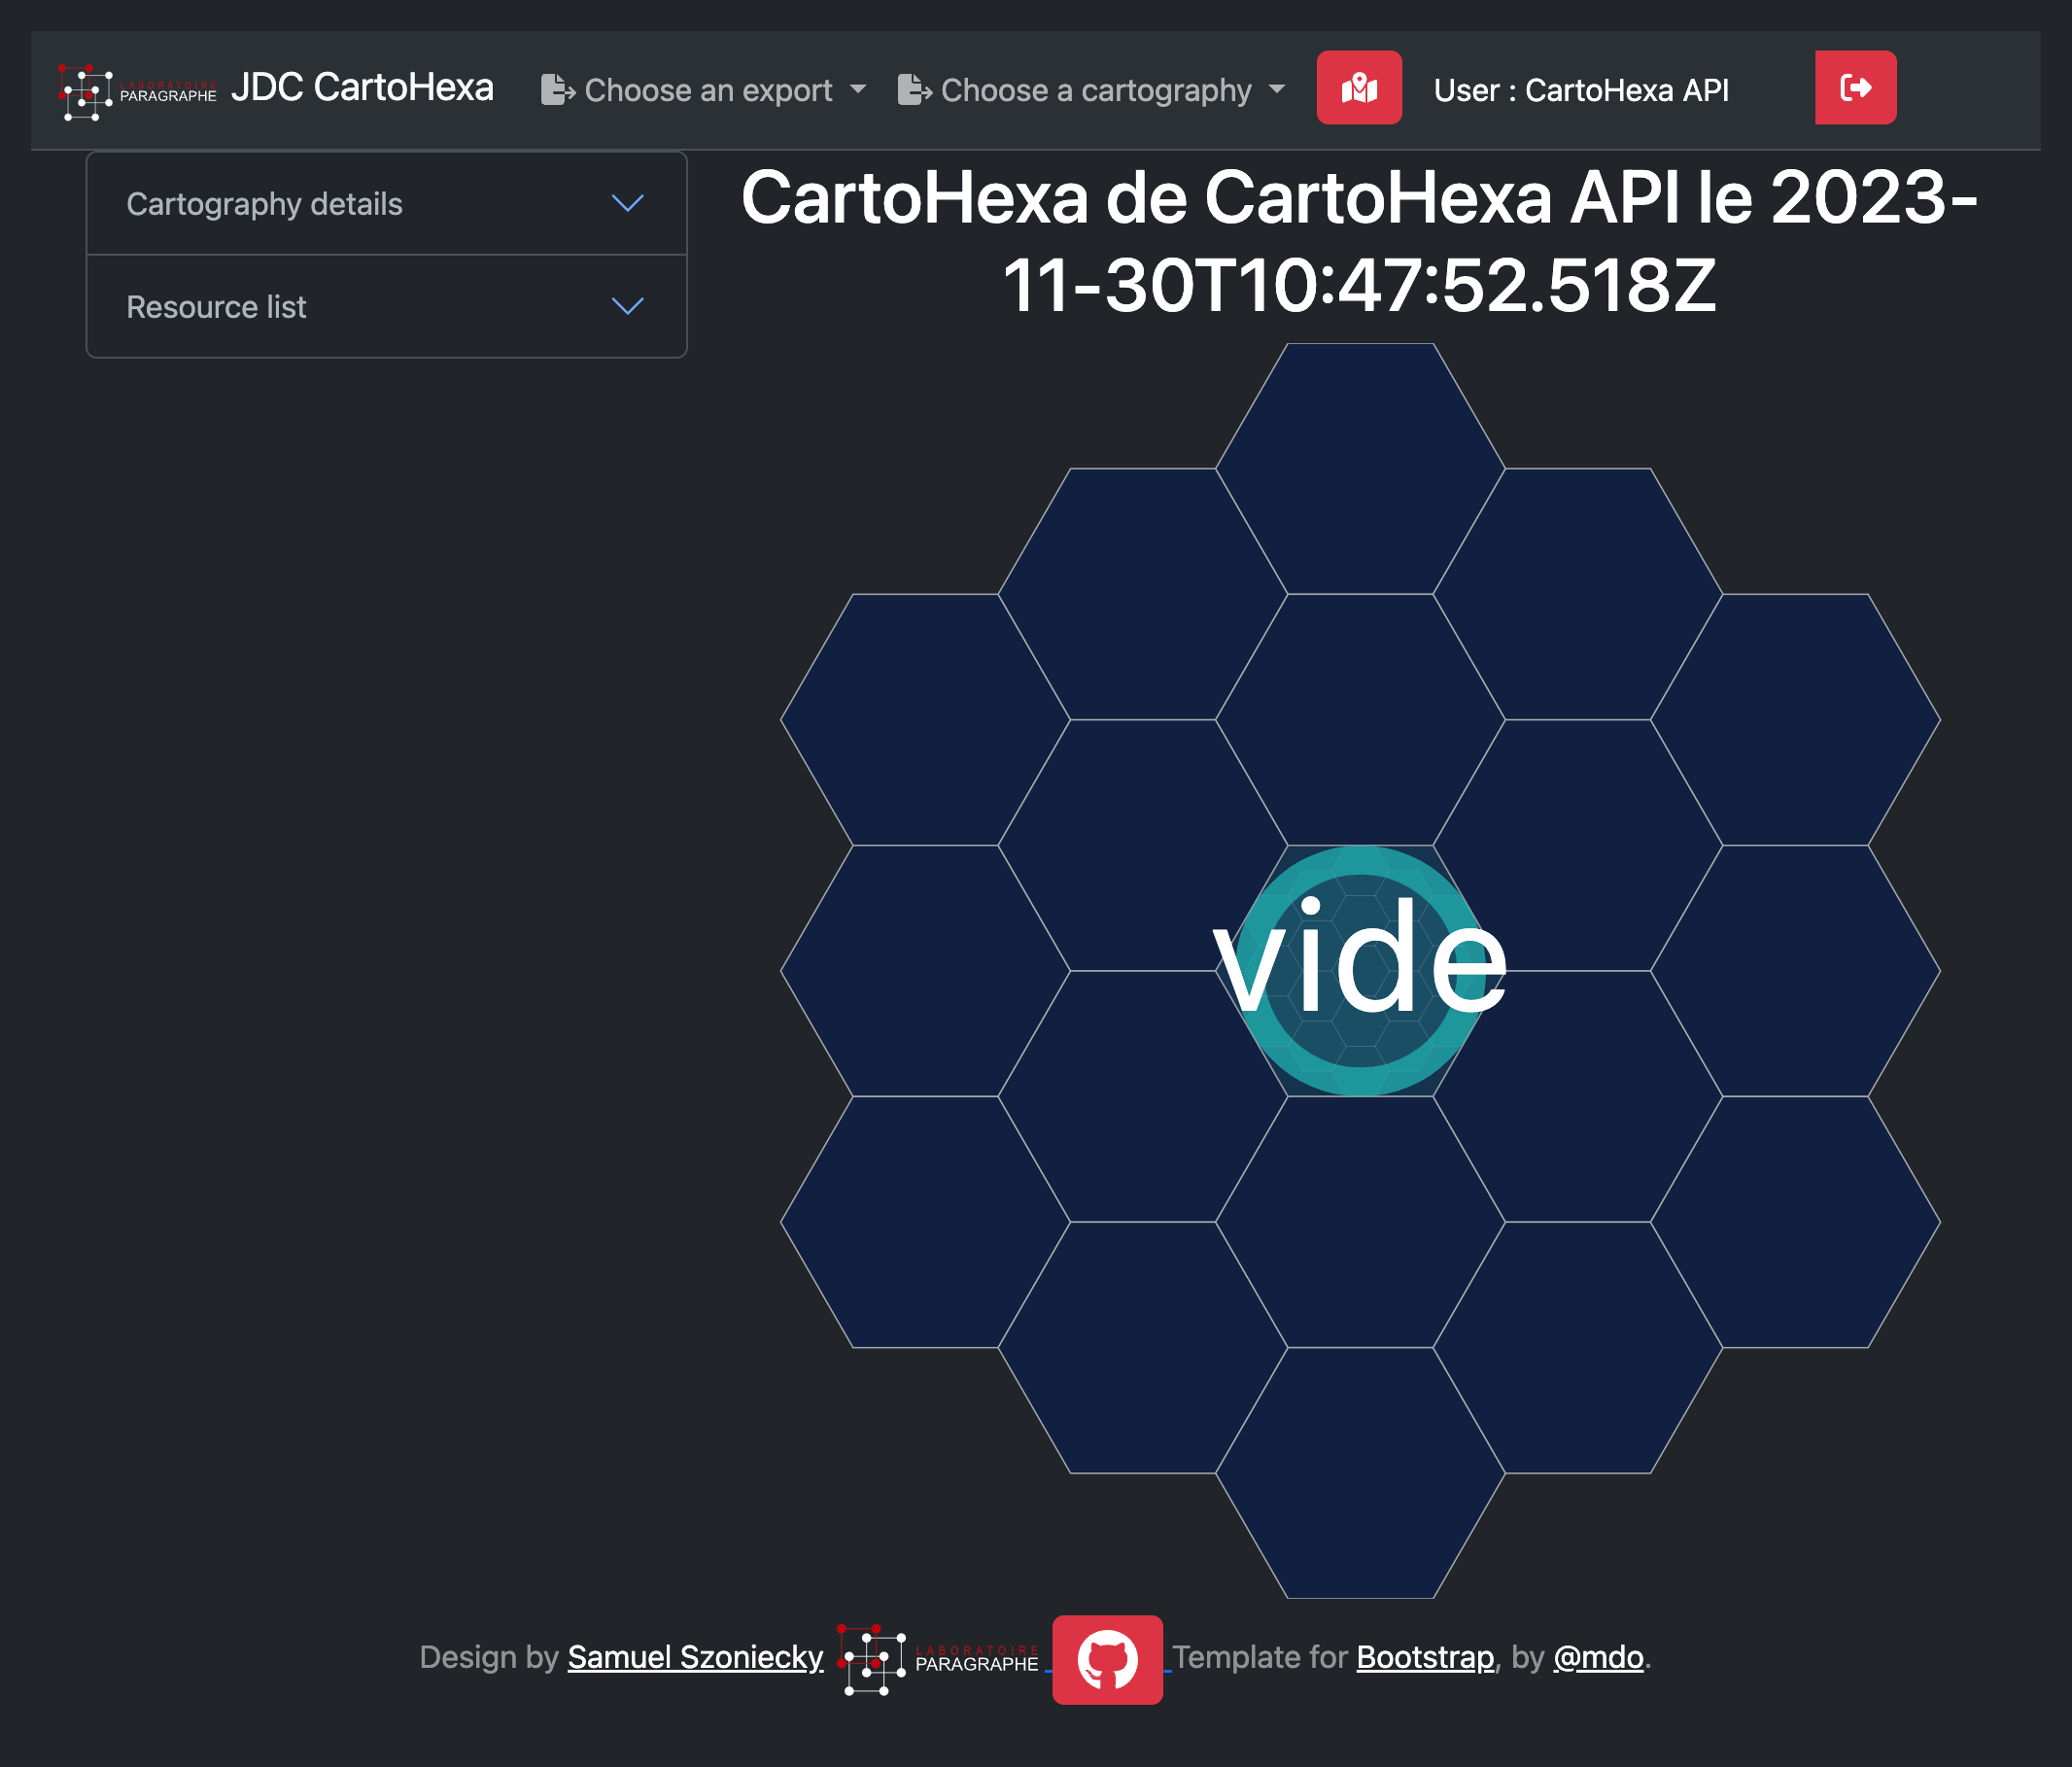
\includegraphics{images/localhost_samszo_HDR_docs_jdcCartoHexa.html.png}

}

\caption{\label{fig-cartoHexa}Cartographie conceptuel dans un espace
hexagonal}

\end{figure}%

Les utilisateurs peuvent ensuite utiliser les applications d'adhérence
que nous venons de présenter, qui consiste par exemple à
«~conceptualiser~» un espace en lui donnant un titre. Il suffit de
cliquer dans l'espace conceptuel pour choisir une position et faire
apparaître un formulaire permettant de saisir le titre du concept. Il
est important de pouvoir créer tous les concepts possibles à partir de
n'importe qu'elle chaîne de caractères car une des difficultés bien
connues dans l'usage des ontologies ou des vocabulaires formalisés est
de trouver la «~bonne~» référence dans un ensemble souvent très vaste
dont on ne connaît pas l'ensemble des références et surtout quand on ne
trouve pas d'équivalent à ses propres habitudes linguistiques. C'est
pourquoi, dans nos principes de cartographie des espaces conceptuels,
l'expression des concepts est libre comme c'est le cas dans les
folksonomies (Broudoux, François, Dominique, Cécilia, \& Clotilde,
2012). Toutefois, lors de la saisie du titre du concept, un processus
d'auto-complétion du champ de saisie renvoie les concepts déjà
enregistrée dans la base de données à partir de quelques lettres~;
l'utilisateur est informé des concepts existants et peut donc choisir
une référence que d'autres utilisateurs ont déjà utilisé ce qui permet
de créer une interopérabilité formelle. Notons que cette
interopérabilité ne présage pas d'un consensus sur le sens du concept,
toutefois elle est grandement utile pour rassembler les différents
acteurs qui l'utilise afin qu'il discute de leurs accords et divergences
Section~\ref{sec-axeFormaConsensus}.

L'application «~conceptualiser~» enregistre dans une base de données
Omeka S la position d'un concept défini par un actant ici et maintenant
dans un espace conceptuel de référence en décomposant ces informations
dans les propriétés suivantes~:

- identifiant de la position

- titre de la position

- identifiant de l'espace de référence

- coordonnées de la position dans l'espace de référence

- identifiant de l'actant

- date du choix de la position

- lieu du choix de la position

Décomposer l'actant, le concept et sa position a pour avantage de
partager un concept commun avec d'autres utilisateurs tout en conservant
le point de vue de l'actant sur ce concept. Ainsi, «~aimer~» et «~haïr~»
peuvent être commun à plusieurs personnes mais la distance entre ces
deux concepts peut varier suivant les individus, le temps,
l'espace\ldots{} Il y a donc une dé-corrélation entre le concept et ses
usages. Le concept est virtuel, c'est une potentialité qui s'actualise
dans une «~action située~» c'est à dire dans des usages ayant leurs
propres spécificités ((\textbf{actionSitue?})). De plus,
l'enregistrement situé des étapes de construction de la carte rend
accessible le processus créatif de son auteur.

Cette définition minimale de l'espace prétopologique peut être enrichie
par d'autres applications qui enrichissent l'espace de nouvelles
propriété comme celui qui est à l'œuvre avec IEML. Cette activité
purement conceptuelle consiste à affiner la cartographie en définissant
des rapports entre les concepts à la manière de ce qui se fait lorsqu'on
développe une ontologie (Bruno. Bachimont, 2007) en utilisant par
exemple des propriétés de relation issu du vocabulaire SKOS (Isaac,
2011).

Dans notre cas, l'application «~intérieur~» va nous permettre de définir
les espaces conceptuels à l'intérieur d'autres espaces conceptuels en
suivant la définition~:

\begin{quote}
«~Soit une application i : P(E) → P(E) appelée intérieur et définie
comme suit :\\
∀A, A ⊆ E l'intérieur de A, i(A) ⊆ E est telle que :\\
-- i(A) = {[}a(A\textsuperscript{c}){]}\textsuperscript{c} (P1)\\
-- i(A) ⊆ A (P2)\\
avec A\textsuperscript{c} le complémentaire de A soit E − A.~»
(Levorato, 2008, p. 40)
\end{quote}

Pour utiliser cette application, il suffit de cliquer dans un des
hexagones de la grille pour faire apparaitre un formulaire permettant de
choisir un concept et les relations que ce concept entretient avec le
concept dont il est un sous espace. Ces relations sont exprimées avec le
vocabulaire des relations de SKOS\footnote{\begin{quote}
  Pour une présentation des relations sémantiques dans SKOS~:
  \url{https://www.w3.org/TR/skos-reference/\#semantic-relations/}
  \end{quote}} mais sans toutefois limiter les possibilités
d'associations aux contraintes logiques. Par exemple, il est illogique
que deux concepts possèdent à la fois une relation hiérarchique ``plus
spécifique'' (skos:narrower) et une relation ``plus générique''
(skos:broader). Toutefois, il nous semble important de laisser la
possibilité aux usagers d'exprimer ces relations illogiques afin de
laisser une place aux incohérences et aux inventions poétiques.

\begin{figure}

\centering{

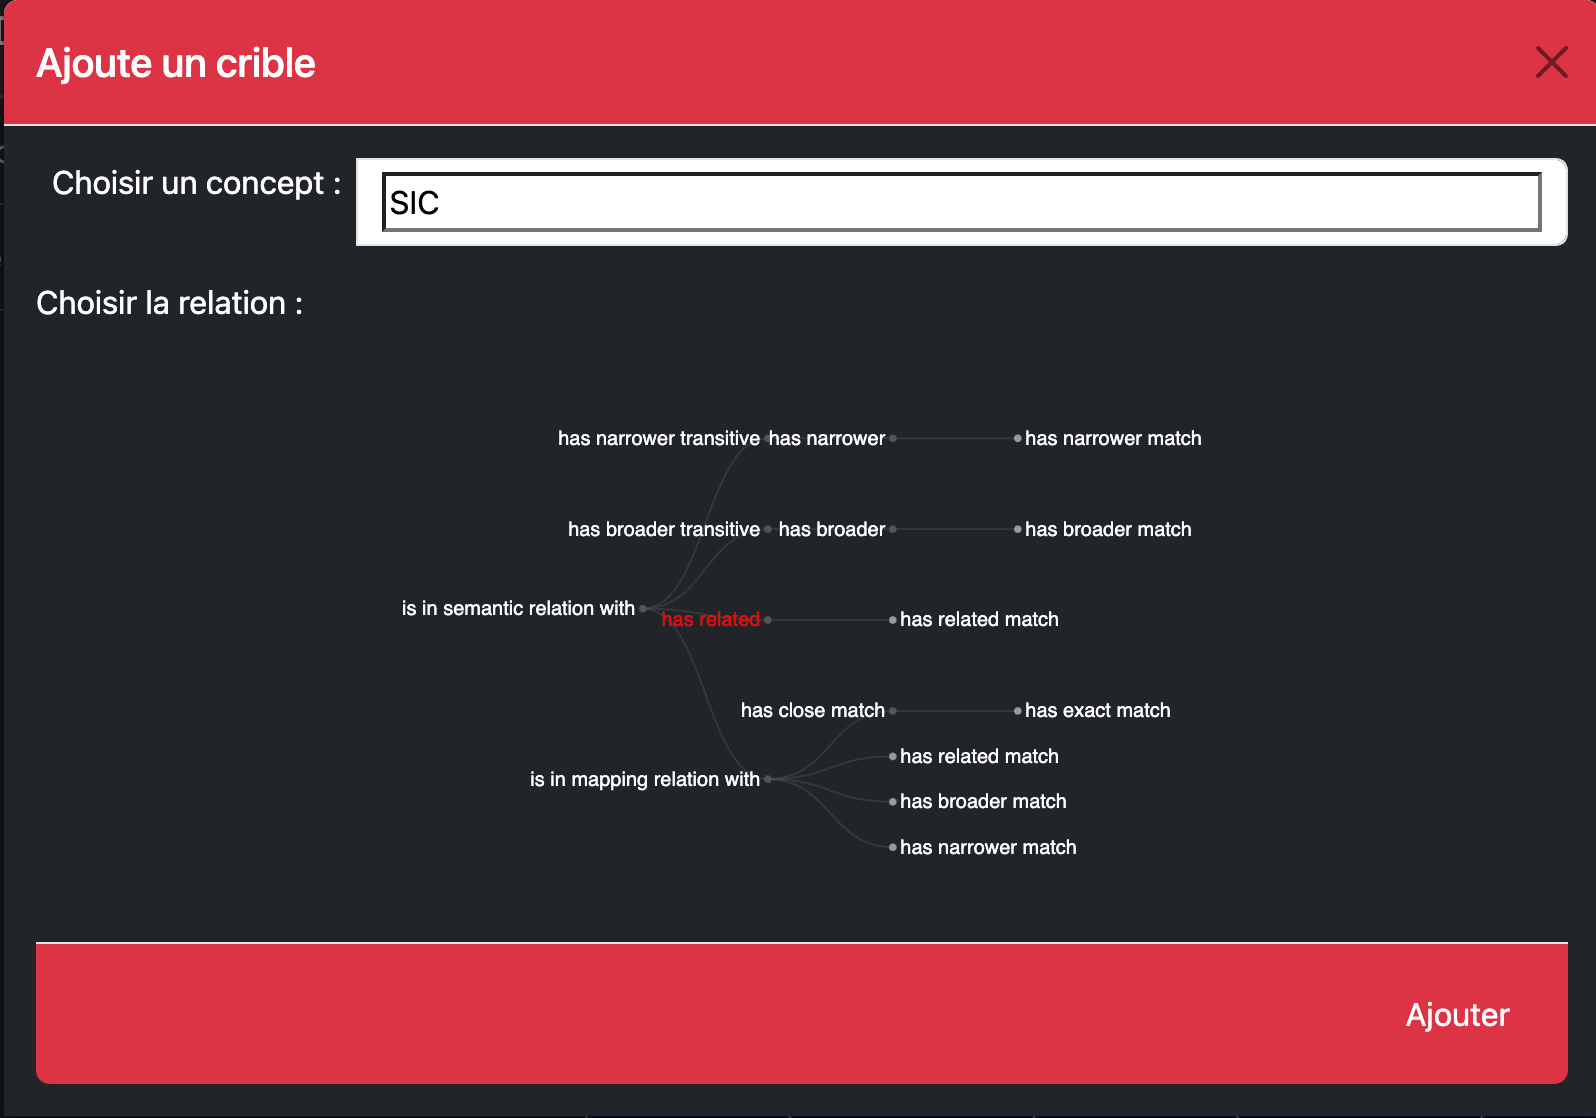
\includegraphics{images/localhost_samszo_HDR_docs_jdcCartoHexaAjoutCrible.html.png}

}

\caption{\label{fig-cartoHexaAjoutConcept}Ajout d'un concept et de ses
relations}

\end{figure}%

\section{L'actant : connaissances des dynamiques
génératives}\label{sec-espaceActant}

Entre la dimension des physicalités organisée en hiérarchies et celle
des concepts organisée en topologies, la dimension des actants organise
l'espace des connaissances à la fois sous la forme de topos et de chôra
(Derrida, 1997; Zamora, 2003). Topos et chôra sont deux manières
complémentaires de définir l'espace soit pour le topos sous la forme
d'une identité par exemple ``Université Paris 8'', soit pour la chôra en
définissant ce que le lieu génère comme activités, ce que sont ses
dynamiques génératives, par exemple dans le cas de Paris 8 : recherches
et enseignements.

\begin{quote}
«~la chôra {[}\ldots{]} relèvent du monde sensible, non du monde
intelligible. Inversement, la notion de topos, dans la mesure où elle
concorde avec la logique de l'identité du sujet, relève moins de la
sensibilité que de l'intelligibilité.~» (Berque, 2009a, p. 232).
\end{quote}

Il est curieux de voir que dans l'histoire, topos et chôra se sont
développés à travers deux manières d'êtres au monde (Latour, 2012a). On
pourrait par exemple voir d'un coté une vision occidentale du topos dont
les modernistes sont les héritiers et qui plonge ces racines chez
Platon, Aristote et que l'on trouve aussi dans la Bible où la première
activité de l'homme est de nommer les vivants pour définir leur identité
:

\begin{quote}
«~2.19 : L'Éternel Dieu forma de la terre tous les animaux des champs et
tous les oiseaux du ciel, et il les fit venir vers l'homme, pour voir
comment il les appellerait, et afin que tout être vivant portât le nom
que lui donnerait l'homme.

2.20 : Et l'homme donna des noms à tout le bétail, aux oiseaux du ciel
et à tous les animaux des champs » (Jérusalem, 1993, p. 19).
\end{quote}

\begin{figure}

\centering{

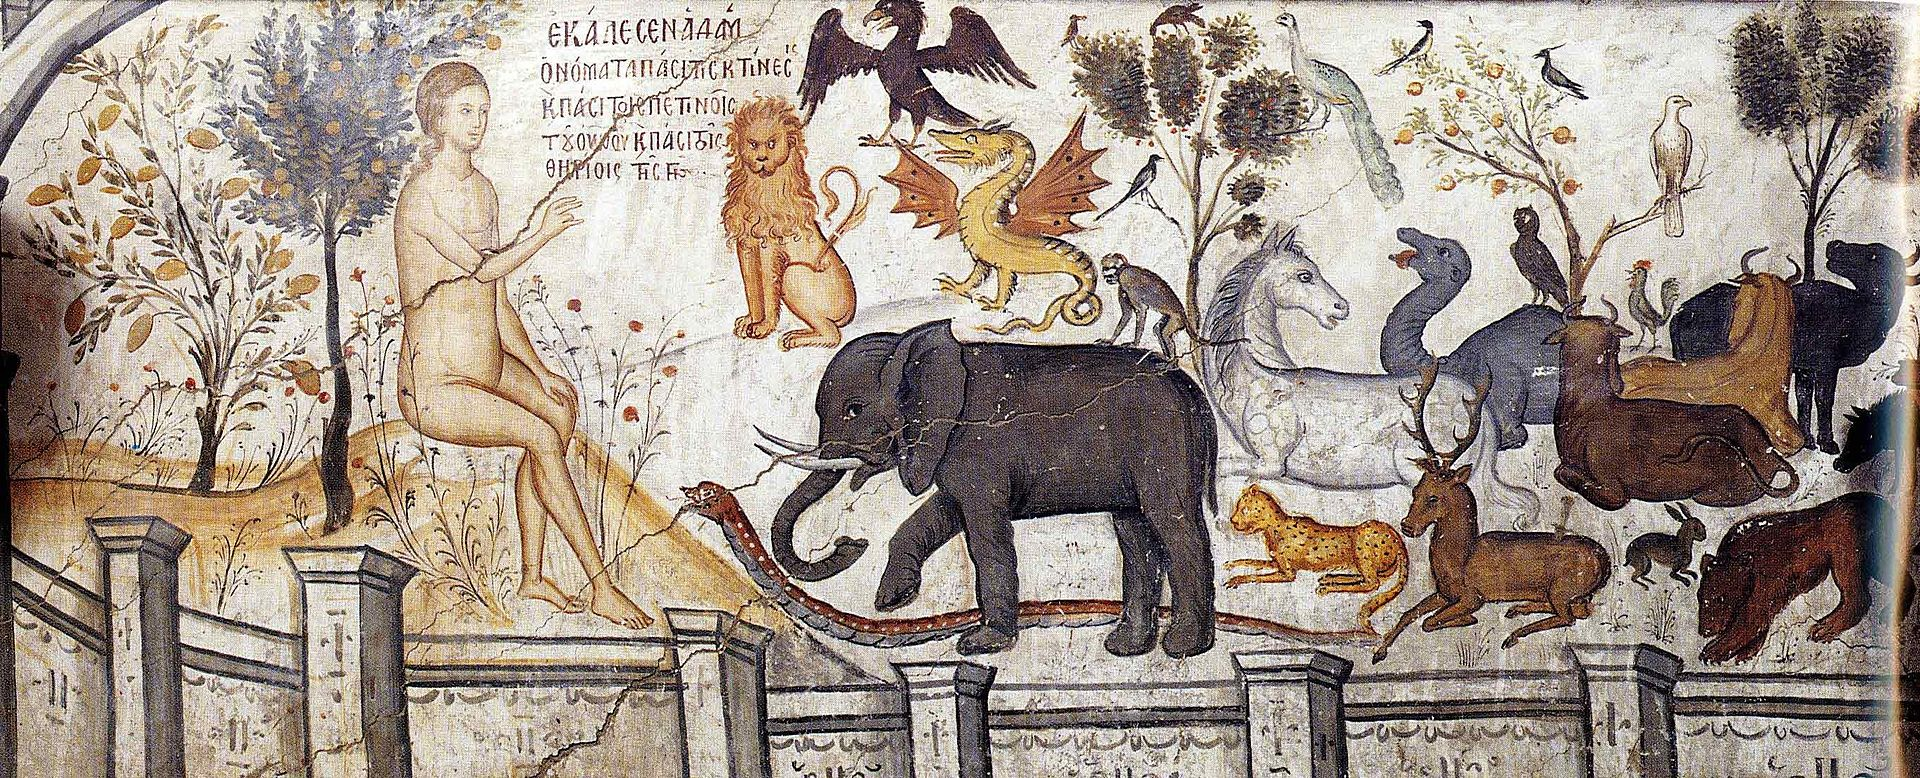
\includegraphics{images/Adam_naming_animals_-_Moni_Ayou_Nikolaou_(Meteora).jpg}

}

\caption{\label{fig-adamNomme}Adam nomme les animaux}

\end{figure}%

Le topos fonde « en Occident la logique du tiers exclu~» (Berque, 2009a,
p. 145) et caractérise les approches Naturalistes dont l'ambition est de
décrire le monde de manière universelle (Philippe. Descola, 2005). Du
coté de l'Orient, la taoïsme apporte quant à lui une approche de
l'environement informationnel différente. Elle ne se base pas sur le
nommage de l'identité mais sur l'expérience des flux informationnels,
des dynamiques génératives qui caractérisent la chôra, comme en témoigne
Lao Tseu six siècles avant notre ère dans les deux premiers paragraphes
du Tao Te King où il insiste sur le caractère indicible du Tao :

\begin{quote}
«~ 1. Le tao exprimable n'est pas Le Tao. 2. Le nom énonçable n'est pas
Le Nom. » (Saint Girons, 2016).
\end{quote}

L'opposition entre ces deux approches trouvent aujourd'hui une actualité
flagrante entre une IA symbolique qui fonctionne par nommage très précis
des identités informationnelles sous la forme d'ontologies et une IA
connexionniste qui privilégie l'émergence de modèle par des cycles
récurrents d'apprentissages (Masure, 2023). Entre identité et
dynamiqmes, les deux approches sont complémentaire notamment quand on
cherche à modéliser les actants qui ne sont ni réductibles à leur
identité ni à leurs activités. L'actant possède une identité qu'on
défini basiquement par un nom et donc par une physicalité mais l'actant
est aussi producteur d'activités et donc de dynamismes génératifs en
créant des rapports entre des physicalités et des concepts
(Section~\ref{sec-rapportsInstExis}). Les actants sont topos de part les
rapports qu'ils entretiennent avec les physicalités et chôra dans les
processus internes d'émergence des connaissances intuitives issu des
expériences de l'espace vécu. L'actant est donc le milieu de ces
pulsations exitentielles que nous décrivions plus haut
Figure~\ref{fig-dynamiquesPulsationsExistentielles}, il est le continuum
entre les physicalités et les intériorités. Modéliser l'actant consiste
donc à une double démarche à la fois de définition de son identité par
des noms et de caractérisation des ces pouvoirs génératifs spécifiques
(dicerner, raisonner, agir). En se sens la représentation de l'actant
est à la fois topologique et chorématique(Brandt, 2021; Reymond \&
Brunet, 1996).

Pour représenter les actants, nous avons fait le choix de l'hexagone
dont la forme est entre le rectangle qui représente les physicalités et
le cercle qui représente les concepts. De plus, les six cotés de
l'hexagone offrent une possibilité de trois plage de connexion vers le
haut où sont représentées les physicalités et trois plages de connexion
vers le bas où l'on trouve les concepts. L'hexagone est une forme qui
peut être utilisée pour paver l'espace de manière fractale puisque
l'intérieur de l'hexagone peut lui aussi être paver avec des hexagones
(Figure~\ref{fig-cartoHexa}). A l'hexagone nous avons associé un cercle
qui défini l'intériorité d'un actant (Figure~\ref{fig-actantP8}) ou de
plusieurs actants qui se partagent la même intériorité par exemple dans
le cadre d'une institution ou d'un groupe d'individu qui mettent en
commun des concepts et des pouvoirs (Figure~\ref{fig-actantP8-membres})
ou dans le cas d'une modélisation global d'un écosystème qui possède sa
propre intériorité composée de plusieurs actants ayant eux-même leurs
propres intériorités (Figure~\ref{fig-actantSonar}).

\begin{figure}

\centering{

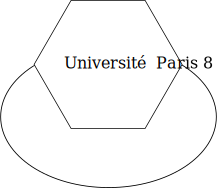
\includegraphics{index_files/mediabag/images/actantP8.pdf}

}

\caption{\label{fig-actantP8}Actant individuel}

\end{figure}%

\begin{figure}

\centering{

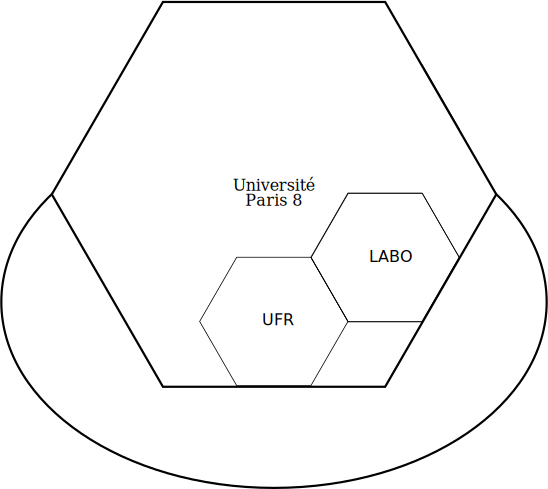
\includegraphics{index_files/mediabag/images/actantP8-labos-ufr.pdf}

}

\caption{\label{fig-actantP8-membres}Actants d'une communauté}

\end{figure}%

\begin{figure}

\centering{

\includegraphics{images/iceSonar.png}

}

\caption{\label{fig-actantSonar}Actants dans un écosystème}

\end{figure}%

Un des autres grands intérets d'utiliser des structures hexagonales pour
modéliser les actants de l'écosystème de connaissances vient du fait
qu'il est possible de créer des formules logiques par positionnement des
hexagones les uns par rapport aux autres. Voici par exemple comment
utiliser des hexagones pour créer des diagrammes de Venn (Coumet, 2020;
Venn, 1866)afin de modéliser l'intersection entre deux, trois et quatre
ensembles d'actants :

\begin{figure}

\centering{

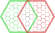
\includegraphics{index_files/mediabag/images/actantVenn2.pdf}

}

\caption{\label{fig-hexaVenn2}Diagramme de Venn à 2 ensembles
=\textgreater{} 3 espaces hexagonaux}

\end{figure}%

\begin{figure}

\centering{


\includegraphics{index_files/mediabag/images/actantVenn3.pdf}

}

\caption{\label{fig-hexaVenn3}Diagramme de Venn à 3 ensembles
=\textgreater{} 7 espaces hexagonaux}

\end{figure}%

\begin{figure}

\centering{

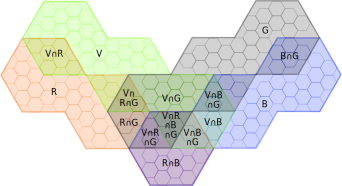
\includegraphics{index_files/mediabag/images/actantVenn4.pdf}

}

\caption{\label{fig-hexaVenn4}Diagramme de Venn à 4 ensembles
=\textgreater{} 15 espaces hexagonaux}

\end{figure}%

Chaque espace défini par les intersections renvoie un ensemble
particulier d'actant, par exemple Figure~\ref{fig-hexaVenn2} modélise
les actants qui appartiennent à l'institution Verte, à l'institution
Rouge et ceux qui sont à la fois dans l'une et dans l'autre. Les
diagrammes de Venn sont très pratiques pour avoir une vision d'ensemble
de toutes les possibilités d'inclusion de plusieurs ensembles.
Toutefois, lorsque le nombre d'ensemble est supérieur à cinq, il devient
difficile de lire correctement certain cas d'inclusion comme le montre
Figure~\ref{fig-hexaVenn4} et même très difficile de les représenter
sous forme hexagonale. Dans le cas où les ensembles d'actant sont
nombreux, il convient donc de trouver d'autres solutions graphiques pour
représenter l'appartenance d'un actant à une institution, par exemple en
représentant une autre dimension existentielle : les rapports.

\section{Les rapports : connaissances des existences
potentielles}\label{sec-rapportsInstExis}

Les rapports sont la quatrième dimension de l'existence que nous
utilisons pour modéliser les écosystèmes de connaissances. Ils composent
la dimension existentielle qui relie les trois autres dimensions, les
connaissances et les espaces qui leurs sont associés : dimension
physique, connaissances des chocs et espaces matériels hiérarchiques,
dimension des concepts, connaissances des essences et espaces
topologiques, dimension des actants, connaissances des dynamismes et
espaces topographiques chorématiques. Les rapports définissent des
espaces temporels, ils transforment une virtualité en actualité. Par
exemple, je suis en tant qu'actant actuellement en rapport avec la
physicalité de mon clavier et de mon écran qui produisent les concepts
que vous lisez. Ces rapports, ne seront plus actuels quand à la fin de
cette séance de travail je commencerais une autre activité. Moi en tant
qu'actant, mon clavier en tant que physicalités et ce que j'ai écrit en
tant que concepts, nous existons toujours comme potentialités de futurs
rapports qui s'instancieront à une date et pour une période données. En
d'autres termes, les trois dimensions physique, actant, concept créent
des potentialités de rapports qui s'instancient ici et maintenant dans
l'actualité d'une existence informationnelle.

Pour modéliser des rapports le modèle hypertextuel basique : nœud -
ancre - lien et depuis longtemps utilisé (Balpe et al., 1996) de même
que le triplet RDF sujet - objet - prédicat (Gandon, Faron-Zucker, \&
Corby, 2012) que le W3C préconise pour modéliser des rapports logiques
en RDF{[}\^{}principecarto-37-1{]}. Ils sont traditionnellement
représentés sous la forme d'un graphe où le sujet et l'objet sont des
entités et le prédicat un label décrivant le lien entre les deux entités
: \begin{center}
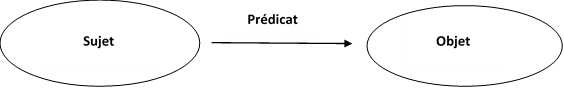
\includegraphics{images/Schema_triplet.png}
\end{center}

Nos principes de cartographie s'accomodent parfaitement de cette
modélisation par triplet RDF mais nous faisons le choix d'un autre type
de représentation qui reprend les recommandations du W3C avec le format
«~Open Annotation~»\footnote{\begin{quote}
  cf.~\url{http://www.openannotation.org/}
  \end{quote}} qui code de façon très simple les relations entre des
ressources numériques afin de définir un point de vue particulier sur
celles-ci. Suivant ce modèle une ``annotation'' est ce qui met en
rapport un ``body'' à une ``target''. De notre point de vue, la
modélisation du rapport est donc une ``annotation'' qui dans un ici et
maintenant va mettre en relation deux ressources.

\begin{figure}

\centering{

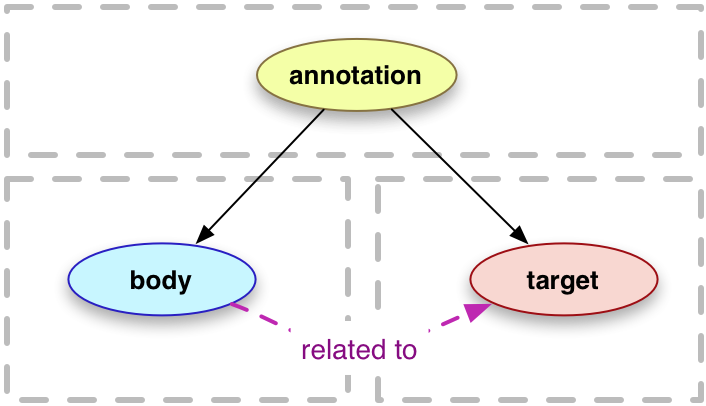
\includegraphics{media/10000001000002C2000001965EFA665F8AB6D163.png}

}

\caption{\label{fig-webAnnotation}Web Annotation Data Model
https://www.w3.org/TR/annotation-model/}

\end{figure}%

Les recherches menées en théories des graphes (Moretti, Jeanpierre, \&
Dobenesque, 2008) ont montré leur souplesse dans la capacité de mettre
en relation des éléments hétérogènes les uns avec les autres où :
\textgreater{} «~la réalité abordée est réduite à des symboles sans
signification pour être soumise à des manipulations aveugles. » (B.
Bachimont, 2020).

Nous défendons ici une toute autre approche puisque la modélisation des
rapports que nous proposons s'incrit dans une démarche où ne reduisons
pas les objets que nous manipulons uniquement à des symboles mais nous
les associons à une «~organologie générale » (Stiegler, 2005) où chaque
élément appartient à une dimension existentielle qui contraint les
manières de le décrire et des le mettre en rapport avec d'autres.
Potentiellement, il est possible de mettre en rapport n'importe quelle
ressource avec n'importe quelles autres quel que soit la dimension
existentielle à laquelle elle appartient. Notre modèle propose quatre
dimensions existentielles et trois positions pour définir un rapport ce
qui donne 4*4*4 = 64 possibilités de rapports. Toutefois, de notre point
vue, ces 64 possibilités de rapport ne sont pas toutes cohérentes comme
le résume le tableau suivant :

\begin{figure}

\centering{

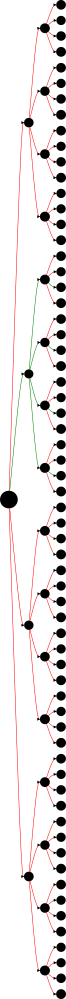
\includegraphics{images/coherencesRapports.png}

}

\caption{\label{fig-coherenceRapport}Cohérences des rapports}

\end{figure}%

On le voit, la majeur partie des relations sont pour nous incohérentes
puisque sur 64 possibilités nous n'en retenons que 9. Insistons sur le
fait que ces incohérences le sont de notre point vue et que d'autres
personnes pourrait considérer que d'autres rapports sont possibles
suivant leurs manières de penser les connaissances. C'est ici que se
situe les débats scientifiques non pas au niveau des techniques
informatiques ou de la justesse mathématique mais au niveau
épistémologique. Nous avons fait le choix de limiter les possibilités
aux cas qui correspondent à l'épistémologie que nous pratiquons
Chapter~\ref{sec-principesCarto} mais de nombreuses questions se posent
: peut-on considérer comme sujet uniquement les actants et comme
prédicat uniquement les concepts ? Les concepts peuvent-ils être des
objets ? Les physicalités peuvent-elles êtres des prédicats ?

Pour toutes ces questions, il convient de trouver des exemples précis
dans la littérature ou dans la vie courante qui montre la cohérence ou
non des rapports. Nous nous appuyons sur notre modèle
Section~\ref{sec-modeleOntoEthique} pour faire une séparation nette
entre les actants comme milieu entre les dimensions des physicalités et
des intériorités, entre les attributs de l'entendu et de la pensée. Nous
posons comme principe de modélisation que l'objet est une physicalité,
que le prédicat est un concept et que le sujet est un actant. Attention,
ces restrictions n'empèchent pas de considérer une personnes comme un
concept comme le fait par exemple la philosophie avec le personnage de
l'idiot ou quand on parle de Napoléon en politique ou dans une fiction.
De même, les physicalités peuvent être conceptualisés pour en parler en
terme générique et pas spécifique, la physicalité banane dans la coupe à
fruit sur la table, devient alors banane en tant que fruit jaune et
allongée des zones tropicales. Il est toujours possible de modéliser une
entité suivant un dimension particulière afin de s'interroger sur un
point de vue spécifique. C'est ce qui et à l'oeuvre dans l'hypothèse
Gaïa qui pense notre Terre non plus uniquement comme un ensemble de
physicalités mais comme actant (Latour, 2015). C'est aussi ce que font
les poètes en transformant des concepts ou des émotions en actants
autonomes. Globalement, la transformation d'une dimension physique ou
conceptuelle en actant est un processus d'agentivité (Hörl \& Plas,
2012; Ingold, n.d.) qui est de la responsabilité du modélisateur dont
les choix orientent explicitement ses analyses vers un mode d'existence
spécifique :

\begin{quote}
«~sujet et objet, loin d'être au début de la réflexion comme les deux
crochets indispensables auxquels il convient d'attacher le hamac où va
pouvoir somnoler le philosophe, ne sont que des effets assez tardifs
d'une véritable histoire des modes d'existence » (Latour, 2009, p. 5)
\end{quote}

Pour gérer, ces informations dans la base de données nous avons utilisé
le module Omeka S ``Annotation'' développé par Daniel
Berthereau\footnote{\begin{quote}
  Accessible ici~:
  \url{https://gitlab.com/Daniel-KM/Omeka-S-module-Annotate}
  \end{quote}} afin de créer des rapports entre des ressources
physiques, actants et concepts. Notons que cette modélisation est elle
aussi fractale puisque un rapport en tant que ressource peut être en
relation avec les autres dimension existentielles, par exemple pour
qualifier le rapport avec un concept particulier, comme ceux proposés
par la langage SKOS Figure~\ref{fig-cartoHexaAjoutConcept}.

Pour représenter les rapports dans nos diagrammes de visualisation des
complexités existentielles, nous utilisons des lignes avec un début sous
forme de cercle vert correspondant à l'objet, un milieu sous forme de
carré blanc correspondant au sujet et une fin sous forme de flèche rouge
correspondant au prédicat. Ce choix de représentation est motivé par la
forme générique d'une existence informationnelle où le centre est occupé
par l'actant qui dans nos contraintes de possibilité des rapports est
toujours le sujet.

\begin{figure}

\centering{

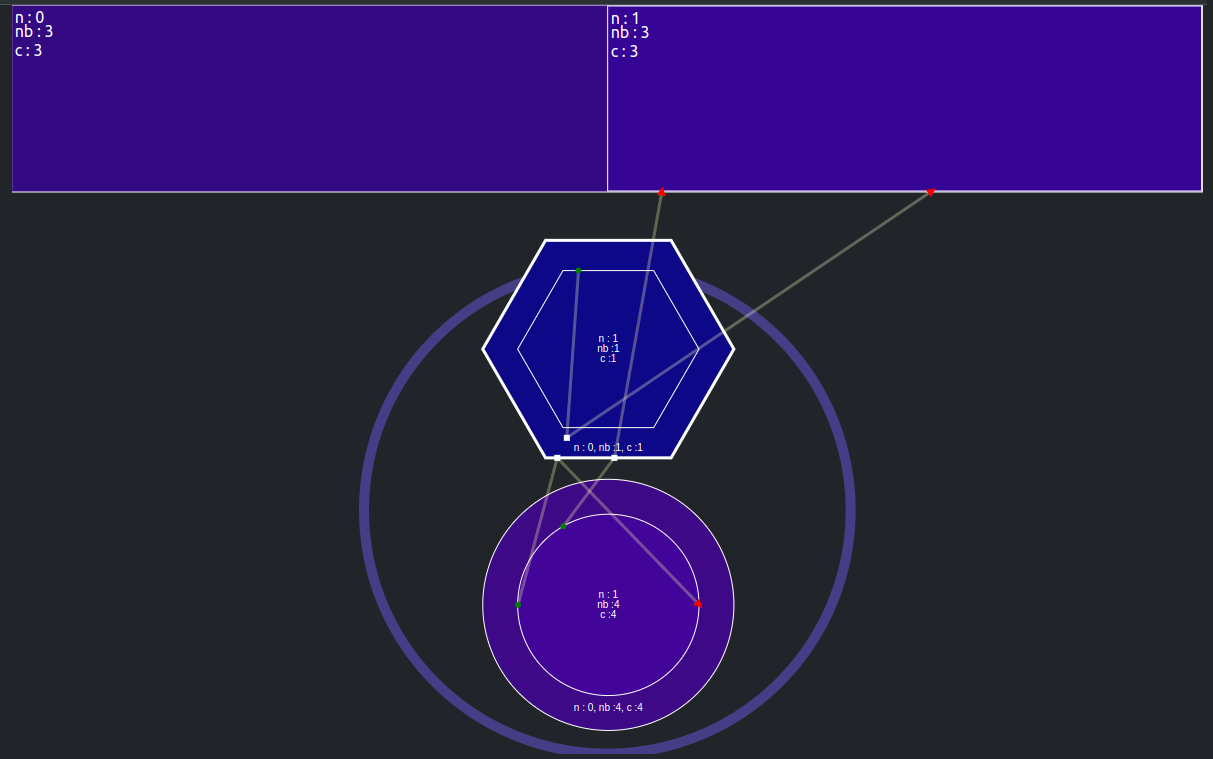
\includegraphics{images/localhost_samszo_HDR_jdcComplexityDiagramme.html.png}

}

\caption{\label{fig-datavizRapport}Visualisattion des rapports}

\end{figure}%

Les quatre dimensions de l'existence que nous utilisons pour modéliser
les écosystèmes de connaissances, sont autonomes quant à leur propriétés
spécifiques et leur mode de représentation. Toutefois, ils convient de
les utiliser ensemble pour obtenir une vision globale de l'écosystème.
Pour cela, nous avons besoin d'un nouveau principe pour associer ces
dimensions existentielles et les représenter : le crible.

\section[Modéliser des cribles~: vers une cartographie des
subjectivités]{\texorpdfstring{Modéliser des cribles~: vers une
cartographie des
subjectivités\footnote{Ce chapitre reprend en les modifiant les
  chapitres consacrés au crible dans (Szoniecky, 2020)}}{Modéliser des cribles~: vers une cartographie des subjectivités}}\label{sec-modeliserCrible}

Définir des principes de cartographie et choisir des modèles efficaces
ne suffisent pas pour modéliser un écosystème de connaissances
respectueux des différents points de vue et de leurs évolutions. Il est
aussi nécessaire de concevoir une méthodologie pour récolter des données
dont on peut évaluer les dimensions objectives et subjectives,
c'est-à-dire celles qui dépendent du choix d'un individu et celles qui
utilisent des systèmes de référence reconnus. Pour reprendre les mots de
Guattari, notre objectif est de concevoir des «~cribles~» afin de
produire des données dont on peut discerner le subjectif et l'objectif~:

\begin{quote}
«~ dans tous les registres des cribles se constituent en interface entre
1) les virtualités virulentes du chaos, les proliférations stochastiques
et 2) les potentialités actuelles dûment répertoriables et
consolidables.~» (Guattari, 1992, p. 140)
\end{quote}

Le crible filtre les flux d'informations dans un «~fourmillement de
petites inclinaisons~» qui composent un «~tissu de l'âme~» (G. Deleuze,
2003) interface entre le monde et l'individu~:

\begin{quote}
«~ le monde entier n'est qu'une vitualité qui n'existe actuellement que
dans les plis de l'âme qui l'exprime, l'âme opérant des déblis
intérieurs par lequel elle se donne une représentation du monde
incluse.~» (G. Deleuze, 1988, p. 32)
\end{quote}

La notion de crible est particulièrement intéressante parce qu'elle
fournit une analogie dont on peut faire une représentation dynamique et
interactive dans le but de concevoir une application de modélisation des
écosystèmes de connaissances. Pour cela, nous simplifierons la
complexité des phénomènes de perception et d'expression que le crible
met en œuvre en le comparant à une passoire dont les trous sont autant
d'indicateurs définissables par une expression logique composée :

\begin{itemize}
\item
  d'un sujet = le flux d'information,
\item
  d'un objet = l'indicateur
\item
  d'un prédicat = l'opérateur de la sélection.
\end{itemize}

Par exemple, dans le cas de l'ustensile de cuisine passoire, les trous
du crible ont comme description~:

\begin{itemize}
\item
  sujet = les pâtes qui cuisent dans l'eau,
\item
  objet = être un fluide,
\item
  prédicat = retient ce qui n'est pas l'objet.
\end{itemize}

Les cribles que nous concevons utilisent ce même principe~: une
interface qui dans un premier temps retient le flux puis le discerne
suivant les expressions qui criblent cette interface. Ce processus est
fractal, en discernant le flux, le crible produit un flux qu'un autre
crible peut discerner et ainsi de suite. À chaque passage du flux
d'information par le crible, l'information se transforme en donnée
c'est-à-dire en une information discernable. En disposant les cribles en
couches successives, on forme un réseau d'expressions logiques dans
lequel les flux d'information passent se transformant ainsi en données
de plus en plus discernables. Cette description correspond tout a fait à
un réseau de neurones artificielles (perceptron) que l'on peut associé
en couche pour développer des systèmes d'apprentissage profond :

\begin{figure}

{\centering 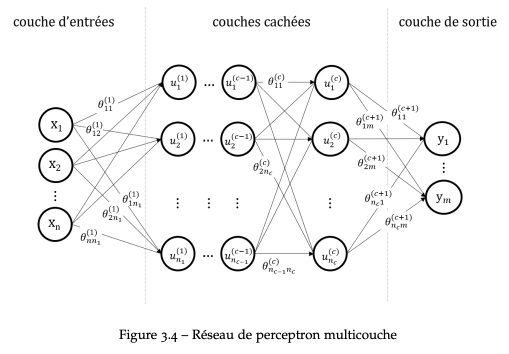
\includegraphics{images/reseaux-neurones.png}

}

\caption{Réseaux de neurones (Nguyen, 2018)}

\end{figure}%

Pour mieux comprendre comment le crible opère en tant qu'interface, nous
le décrivons à la lumière du cycle de la sémiose
Figure~\ref{fig-cyclesemiose}. Le fonctionnement physiologique de la
signification est un cycle continu entre d'un côté le «~monde naturel~»
et une «~élaboration sémiotique~» à travers une interface et un
processus d'anasémiose~: «~un enchaînement de modules, traduisant en
impressions de continuum les phénomènes digitaux du monde~» (µ, Edeline,
\& Klinkenberg, 2015b). Puis d'un autre côté, entre une élaboration
sémiotique et le monde naturel à travers une interface et un processus
de catasémiose défini comme une «~série de traitements par des modules
spécialisés, intermédiaires entre le traitement des informations par le
cortex et les effectuations sur le monde~» (Ibid.). De ce point de vue,
le crible est l'interface qui transforme par un pouvoir de discernement
(anasémiose) le monde naturel en élaboration sémiotique, elle-même
transformée par le crible en pouvoir d'agir sur le monde (catasémiose).
À l'expression «~monde naturel~» utilisée par (µ et al., 2015b), nous
préférons le concept de «~physicalités~» que propose (Philippe. Descola,
2005) pour s'affranchir d'une vision trop «~naturaliste~» d'appréhender
le monde. Selon cet anthropologue, la signification que nous donnons au
monde se conçoit globalement comme la manière dont nous créons des
relations entre des «~physicalités~» et des «~intériorités~». Parmi les
quatre grandes manières de créer ces relations au monde (naturalisme,
animisme, totémisme et analogisme), l'analogisme nous intéresse
particulièrement, car elle considère que le monde se compose en relation
avec un chaos, mais plus encore que ce mode d'existence est celui du
numérique et de l'Internet comme le souligne Michel Serres~:

\begin{quote}
«~ un océan vertigineux et des réseaux de relations toujours en train de
multiplier leurs connexions définit en rigueur l'analogisme, mot qui
résume et peint à merveille notre monde objectif, nos travaux cognitifs,
nos rêves subjectifs ainsi que les collectifs qui naissent aujourd'hui
et feront la politique du futur.~» (Michel. Serres, 2009, p. 85)
\end{quote}

Pour donner du sens à ce monde de chaos, les cribles offrent des réseaux
de correspondances facilitant le travail d'interprétation~:

\begin{quote}
«~ Rappelons que l'identification analogique repose sur la
reconnaissance d'une discontinuité générale des intériorités et des
physicalités aboutissant à un monde peuplé de singularités, un monde qui
serait donc difficile à habiter et à penser en raison du foisonnement
des différences qui le composent, si l'on ne s'efforçait de trouver
entre les existants, comme entre les parties dont ils sont faits, des
réseaux de correspondance permettant un cheminement interprétatif.~» (P.
Descola, 2006, p. 182)
\end{quote}

Concevoir un crible entre objectivité et subjectivité, monde naturel et
délibération sémiotique, physicalités et intérioritéscf, consiste dans
l'univers du numérique à définir une analogie pour modéliser les
cohérences nécessaires à la récolte des données et à leurs
interprétations. Le crible sujet -- prédicat -- objet est une structure
trop simple et beaucoup trop plastique pour réduire suffisamment les
«~proliférations stochastiques~», nous proposons d'enrichir cette
structure avec des règles analogiques supplémentaires qui minimiseront
les réseaux de correspondances et les chemins interprétatifs possibles.

\subsection{Proposition d'un crible}\label{sec-propositionCrible}

En partant de la structure sujet -- prédicat -- objet, nous proposons de
concevoir un crible pour modéliser notre écosystème de connaissances en
nous focalisant sur les références qui composent notre bibliographie.
Globalement, l'analyste devra s'interroger sur les caractères génériques
et spécifiques des niveaux de modélisation. Si tous les éléments qui
composent un niveau sont ressemblants par rapport à un indicateur, ce
niveau est spécifique, il n'est pas nécessaire de le détailler. Par
contre, s'il existe des différences entre les éléments par rapport à un
même indicateur, le niveau est générique, il convient alors de le
détailler en niveaux spécifiques. Par exemple, si j'utilise l'indicateur
«~à comme mot numérique~» et que tous les paragraphes d'un même chapitre
respectent cet indicateur, le niveau chapitre est spécifique, il n'est
pas nécessaire de le détailler en paragraphe. Dans le cas contraire, le
niveau chapitre est générique, il convient de le détailler en paragraphe
pour modéliser ceux qui respectent l'indicateur et ceux qui ne le
respectent pas.

Concernant, l'objet de notre structure basique de modélisation, nous le
considérons uniquement comme la description des dimensions physiques et
des matérialités Section~\ref{sec-espaceMateriels}. L'objet se décrit de
manière arborescente de façon à définir les parties qui composent un
élément. Chaque branche donne des détails supplémentaires sur l'objet
suivant la forme logique~: élément (sujet) -- a pour partie (prédicat) →
sous partie (objet). Par exemple, dans le cas de notre bibliographie, un
des objets de la modélisation est défini par~: livre → chapitre →
paragraphe → phrase → mot →caractère. Le choix des niveaux de détail est
subjectif, il dépend de la finalité que le modélisateur donne à son
travail. Par exemple, pour analyser cette écosystème, il n'est pas
nécessaire de différencier chaque caractères de manière individuel, car
il n'y aura pas de différence signifiante entre ces caractères. En
revanche, connaître les mots apporte des informations intéressantes
notamment concernant le nombre de fois qu'ils apparaissent, ou leurs
usages en cooccurrence avec d'autres mots.

Concernant le sujet de la structure sujet -- prédicat -- objet, nous
proposons de contraindre les possibilités de sa définition aux auteurs
des références Section~\ref{sec-espaceActant}. Ces auteurs ne sont pas
uniquement des individus, mais peuvent être aussi des collectifs suivant
l'appartenance de ces auteurs à des groupes de recherche, des
laboratoires, des universités, des pays dont ils sont citoyens. La
description des sujets reprend le principe de modélisation arborescente
où le lien entre les branches se fait suivant le prédicat «~a pour
partie~», par exemple ~: le chercheur X (sujet) a pour partie (prédicat)
le laboratoire Y (objet). Là aussi, le choix du niveau sera soumis aux
caractères générique et spécifique. Par exemple, il n'est sans doute pas
nécessaire de spécifier les différents membres d'une université qui
participent à la vie d'un laboratoire de recherche. En revanche, il est
utile de préciser le nom des chercheurs qui ont participé à la rédaction
d'un ouvrage car ils apportent un point de vue spécifique. Il est
évident que nous ne réduisons pas les relations des acteurs uniquement à
un rapport de partie et de sous partie, les relations entre les
individus et les collectifs sont bien plus complexes, elles peuvent être
par exemple hiérarchiques, familiales, amicales\ldots{} Dans le crible
que nous proposons cette spécificité des relations est décrite par une
modélisation des rapports entre acteurs par exemple sous la forme~:
auteur 1 (sujet) collabore avec (prédicat) auteur 2 (objet).

Concernant le prédicat de la structure logique que nous utilisons, il
est défini par un concept Section~\ref{sec-espaceConceptuels} qui prend
la forme d'une périphrase plus ou moins complexe par exemple~:
«~écrire~», «~lire~», «~participer à une conférence scientifique~». Le
concept peut lui aussi être détaillé en utilisant par exemple la syntaxe
SKOS pour définir une structuration des éléments conceptuels et de leurs
relations. Notons que cette modélisation des concepts ne se représente
pas uniquement sous la forme d'une arborescence, mais plutôt sous celle
d'une topologie ou pour employer les termes de (Gilles. Deleuze \&
Guattari, 1980) d'un rhizome. Les structures topologiques étant plus
souples, l'organisation des concepts en tant qu'espaces sémantiques est
beaucoup plus plastique et ne se réduit pas à l'arbre, mais se
représente avec une multitude de formes possibles. Il y a par exemple
les diagrammes de Venn, les matrices, les radars, les nuages de tag, les
repères à deux axes\ldots{} Ces représentations définissent leurs
propres systèmes de coordonnées et par la même des espaces sémantiques
particuliers dans lesquels il est possible de se positionner. Ce
principe de cartographie conceptuel est très utilisé pour définir un
domaine de connaissance comme le fait par exemple David Mc Candless avec
sa typologie des idées\footnote{lien vers le diagramme :
  \url{https://informationisbeautiful.net/visualizations/a-taxonomy-of-ideas/}}.

\begin{figure}

\centering{

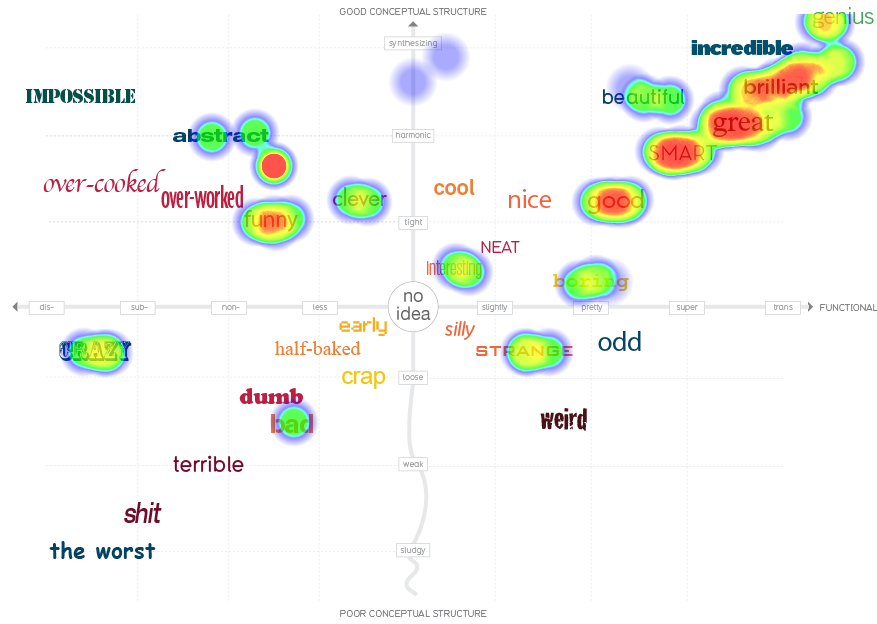
\includegraphics{images/TaxonomyIdeas.png}

}

\caption{\label{fig-TaxonomyIdeas}Taxonomie des idées}

\end{figure}%

Le crible est pour l'instant composé de trois dimensions correspondant
au sujet, à l'objet et au prédicat de la formule logique basique. Chaque
dimension est une collection d'éléments dont nous avons défini les
caractéristiques essentielles. Il nous faut maintenant ajouter une
quatrième dimension correspondant aux rapports
\textbf{?@sec-sec-rapportsInstExis} que ces éléments entretiennent les
uns avec les autres. En effet, suivant notre hypothèse d'un univers
chaotique -- analogiste, toutes les relations entre objets, sujets et
prédicats sont possibles, mais toutes ne sont pas exprimées, uniquement
celles qui sont choisies pour la modélisation . Il est donc important de
définir les rapports comme une des dimensions fondamentales puisqu'ils
existent potentiellement, mais ne sont pas effectuées nécessairement
\textbf{?@fig-contraintesRapports} . Il y a une actualité des rapports,
une temporalité des relations entre les éléments composant la formule
sujet, objet et prédicat, il convient donc de modéliser celles-ci pour
passer d'une signification potentielle du crible à une expression de
cette signification. Les rapports sont l'expression temporelle des
dynamismes du crible à la fois dans le présent, le passé et le futur.
L'expressions d'un rapport se fait dans un présent dont on enregistre la
date pour constituer un historique et simuler les évolutions. Par
exemple, la formule~: «~il (sujet) annote (prédicat) un livre (objet)~»
est effectuée à des moments précis et suivant des répétitions
particulières. Les rapports sont donc génératifs dans la mesure où ils
créent une potentialité d'évolution non seulement dans leurs répétitions
à l'identique, mais aussi dans leurs transformations par mutations des
éléments les constituants. La formule «~il (sujet) annote (prédicat) un
livre (objet)~» peut se transformer en «~il (sujet) annote (prédicat) un
article (objet)~» ou en «~il (sujet) écrit (prédicat) un livre
(objet)~». Ce sera la modélisation qui limitera les évolutions du
rapport en définissant les éléments qui composent les objets, les sujets
et les prédicats.

Le crible que nous proposons pour modéliser notre écosystème de
connaissance est donc composé à partir de la formule logique sujet --
objet -- prédicat que nous avons décomposé en quatre dimensions
possédant chacune leurs contraintes~: - objet~: éléments physiques
structurés en arborescences, - sujet~: éléments sociaux structurés en
collectifs, - prédicat~: éléments conceptuels structurés en topologies,
- rapports~: éléments temporels structurés en triplets.

\subsection{Usages du crible}\label{sec-usageCrible}

Le crible est à la fois un outil de lecture et d'écriture, il est
utilisé comme grille d'analyse d'un contexte particulier (discerner) et
en même temps comme système d'expression de ce contexte (agir). La
problématique principale de modélisation d'un écosystème de connaissance
\textbf{?@sec-part-cartoConnaissances}, est celle de la récolte des
données de manière à ce qu'elle soit tout à la fois facile pour des
non-spécialistes et utile pour les experts. Utiliser un crible simplifie
la récolte des données, car elle donne une signification très précise à
une expression simple en positionnant cette expression dans la
modélisation du crible qui par la même s'enrichit de nouvelles
informations. Plus le crible sera utilisé, plus la modélisation du cible
sera précise et plus l'expression à travers ce crible sera elle aussi
précise~; dans la mesure où la signification du crible est comprise par
ses utilisateurs. En proposant un crible sur la base de la formule sujet
-- objet -- prédicat, nous facilitons sa compréhension par les
utilisateurs qui retrouvent une expression simple et courante et renvoie
à des questions basiques~: qui~? = sujet, quoi~? = objet, comment~? =
prédicat. Ces expressions sont de plus contextualisées par les
contraintes que nous avons définies pour les quatre dimensions ce qui
limite les interprétations possibles et par la même facilite leur
compréhension. Cette proposition de crible facilite aussi le travail de
récolte des données en le décomposant en tâche simples que l'on peut
attribuer à des personnes ayant le temps et les connaissances
nécessaires pour les faire. Par exemple, décrire qui sont les acteurs
qui participent à une conférence demande de récolter la liste des
participants, de la saisir en la mettant en relation avec l'écosystème.
En revanche, répondre à une question sur l'importance d'une citation est
à la portée de tous et peut se faire dans l'instant. On retrouve ici une
polarisation des informations entre celles qui sont objectives, qui
demandent du temps et des compétences particulières pour exprimer des
données de références, et celles qui sont subjectives et s'expriment
dans l'instant par un choix. Modéliser un écosystème de connaissances
consiste donc à créer un système de références objectives dans lequel
des individus exprimeront des choix subjectifs afin de créer des
rapports dans le système de référence et répondre aux questions : Qui~?
Quoi~? Comment ? En d'autres termes, une modélisation d'un écosystème
produit un environnement relationnel par un dispositif de positionnement
dans un système de référence.

Concernant la position du «~qui~» dans un système de référence objectif,
il est aujourd'hui grandement facilité par les mesures de positionnement
géospatial comme le GPS ou les bases de données de références des
personnes et des institutions comme ISNI (International Standard Name
Identifier\footnote{lien vers le site de l'organisation :
  \url{https://isni.org/}}) qui répondent automatiquement et
objectivement à cette question sauf erreur de la machine, malveillance
ou absence de données. Mais le «~qui~» est plus complexe et ne se réduit
pas à ces positions. Par exemple, dans le cas d'un dispositif numérique,
il renvoie au compte de l'utilisateur qui utilise l'application. Or ce
compte indique juste le login utilisé pour se connecter à l'application,
mais pas quelles personnes ou groupes de personnes l'utilisent. De plus,
dans le cadre du RGPD, il devient nécessaire d'anonymiser ce compte et
donc de limiter son objectivation à une simple référence. Sauf si
l'utilisateur donne un consentement «~libre, spécifique, éclairé et
univoque~»\footnote{lien vers les explications de la CNIL :
  \url{https://www.cnil.fr/fr/les-bases-legales/consentement}}. Dans ce
cas, l'objectivation du «~qui~» devient potentiellement beaucoup plus
précise, car elle peut être mise en relation avec des données
sociologiques voir même physiologiques par exemple en enregistrant le
rythme cardiaque ou l'activité cérébrale lors du processus de
positionnement.

Concernant le positionnement du «~quoi~», là aussi il existe des bases
de données de références qui composent le Linked Open Data (LOD) et
permettent d'adresser des ressources de façon unique et pérenne. Dans le
cas de notre exemple sur la modélisation de notre bibliographie, la base
de données sémantique de la BNF\footnote{lien vers l'explication de
  data.bnf.fr :
  \url{https://www.bnf.fr/fr/recuperer-les-donnees-de-la-bnf-selon-les-standards-du-web-semantique}}
est particulièrement intéressante, car elle offre des références pérenne
et détaillées pour les livres, les auteurs, les concepts. Dans ce cas,
le positionnement du «~quoi~» est relativement complexe puisqu'il est
extrêmement difficile de réduire une référence à une seul expression
comme en témoigne les recherches sur le sens des documents(B. Bachimont,
2020; Lévy, 2023a). Nous proposons d'utiliser une représentation simple
du sens des texte en les représentant sous la forme de nuage de mots
clefs où pour chaque mot l'utilisateur pourra augmenter ou diminuer
l'importance suivant sont propre point de vue. Ce simple rapport, va
générer potentiellement une multitude d'autres rapports, car les
éléments qui le composent renvoient aux informations conservées dans la
base de données comme celles en rapport avec la référence annotée ou
celles de l'utilisateur dont on peut connaître les habitudes
d'annotation voir le parcours scientifique. L'historique de ces
informations et leur multiplication par le nombre d'utilisateurs créent
une base de données très utile pour faire des analyses statistiques ou
pour connaître les informations qui manquent et que d'autres
utilisateurs peuvent ajouter en participant collectivement à
l'enrichissement de cette base de données.

\section{De la confiance dans les données~: vers une cartographie des
affects}\label{sec-confianceDonnees}

Les hypothèses cartographiques que nous venons de poser, précise notre
modèle de description et de représentation des connaissances à partir
duquel nous produisons une foule de données qui, en référence aux
principes basiques du RDF\footnote{\begin{quote}
  \url{https://www.w3.org/RDF/}
  \end{quote}}, sont composées d'un triplet sujet, objet et prédicat,
par exemple : sujet=titre, objet=la vie devant soi, prédicat=est. Si on
en croit les défenseurs du RDF et des technologies qui lui sont associé
pour composer le Web Sémantique, cette formalisation de la connaissance
en brique logiques élémentaires est sensée produire de la confiance
comme en témoigne le fameux «~Semantic Web Stack~»~:

\begin{figure}

\centering{

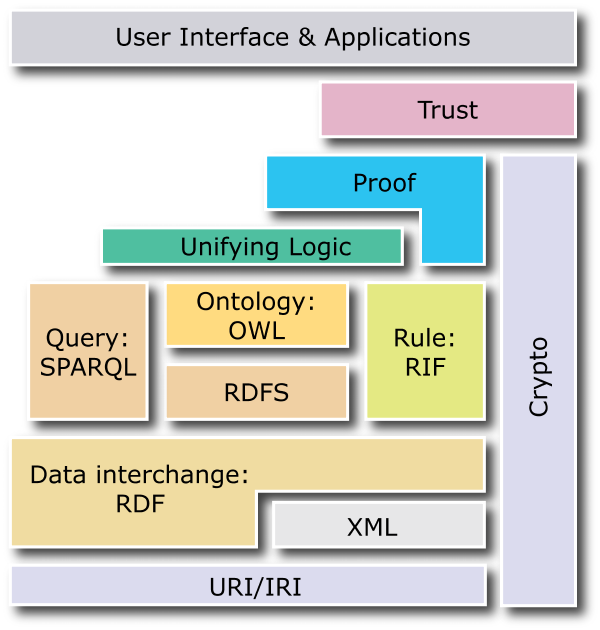
\includegraphics{media/1000000100000258000002762CF3B23905723B38.png}

}

\caption{\label{fig-semanticWebStack}Semantic Web Stack, Par W3C
https://commons.wikimedia.org/wiki/File:Semantic\_Web\_Stack.png}

\end{figure}%

Toutefois, il nous semble que la confiance est toute relative puisque
celle-ci relève d'avantage d'un pari que d'un calcul logique~:

\begin{quote}
«~La confiance se définit donc comme un pari sur les comportements
attendus. Le pari réunit en effet les deux caractéristiques majeures de
la confiance : la relation à l'action {[}\ldots{]}, et la relation à un
futur qui n'est pas encore, mais qui est appréhendé sous la catégorie
des comportements attendus.~» (Hunyadi, 2020a, p. 29)
\end{quote}

A l'heure où la confiance dans les informations est mis à mal par les
phénomènes de dé-information (Bourassa, Larrue, Godin, \& Szoniecky,
2019), il convient d'introduire pour chaque données une évaluation qui
précise qu'elle est le niveau de confiance qu'une personne donne à une
donnée afin de stimuler son esprit critique (Desfriches Doria \&
Meunier, 2021b) en contrecarrant ses penchants naturels~:

\begin{quote}
«~\ldots{} le devenir-libidinal de l'individu guidé par le principe de
commodité l'engage à faire l'économie de la confiance elles-même.
Partout où il le peut, et partout où cela lui est proposé, il tend à
préférer la sécurité assurantielle au pari de confiance.~» (Hunyadi,
2020b, p. 225)
\end{quote}

Plus encore, cette évaluation de la confiance se place dans un objectif
plus large qui consiste à cartographier la réception (Jauss, 1978) d'un
corpus ou pour employer les mots de Bruno Latour de définir les modes
d'existences qui sont en jeu (Latour, 2012b). L'ambition est de
développer un écosystème de connaissances qui présente non seulement des
données mais aussi un point de vue réflexif sur celles-ci. Pour ce
faire, nous avons élaborer un dispositif numérique pour cartographier
les affects (Citton \& Lordon, 2008) d'un collectif par une captation de
la subjectivité des individus qui la compose. Ce dispositif consiste à
fournir aux individus le moyen d'enregistrer la valeur des données
qu'ils consultent. Ainsi, chaque élément du triplet logique RDF qui
compose une donnée, est potentiellement valorisé par la subjectivité
propre à chaque individu au moment de sa consultation. Pour dire
autrement, le dispositif de cartographie des affects capte la
«~pulsation existentielle~» (Berque, 2009b), le pli, qu'un individu
effectue face à une donnée particulière.

Nous avons donc un pli modélisé par le dispositif numérique qui
enregistre le rapport qu'un individu Section~\ref{sec-espaceActant}
exprime entre une donnée du corpus Section~\ref{sec-espaceMateriels} et
une valeur subjective. Cette dernière pourrait être simplement le
concept de confiance que l'individu considère comme présente en cochant
une case ou absente en laissant la case décoché. Pour fournir une valeur
plus subtile, la case à cocher est remplacée par un curseur qui
détermine l'importance de la confiance sur une échelle de 0 à 100. Pour
être plus précis et en adéquation avec les propositions qu'Yves Citton
avancent pour réaliser une cartographie des affects à partir des
principes de Spinoza et Tarde (Citton, 2008a) nous remplaçons l'unique
concept de confiance par un crible Section~\ref{sec-modeliserCrible} qui
décompose la valeur en trois registres~:

\begin{itemize}
\item
  les « valeurs-utilités » qui définissent l'offre et la demande
\item
  les « valeurs-vérités » qui mesurent les gains en connaissances et
  plus largement les phénomènes de croyances, de confiance, les attentes
\item
  les « valeurs-beautés » qui définissent le champ esthétique au sens de
  tout ce qui transforme nos goûts et nos sensibilités.
\end{itemize}

Ces positionnements sur l'importance des valeurs définissent des points
de vue particuliers et des fluctuations temporelles suivant le moment de
leurs expressions. Par exemple, l'évaluation d'une activité peut évoluer
suivant que ses finalités sont accomplies ou non. Si j'annote une
citation pour le plaisir de la découverte et de l'échange, mais qu'une
fois sur deux le plaisir n'est pas là, ce critère devient moins
pertinent alors que celui de la pertinence de la citation ne change pas.
Petit à petit un équilibre se met en place entre l'importance des
valeurs et leurs pertinences dans l'activité.

Le dispositif numérique de cartographie des affects a été implémenté
dans un formulaire que l'utilisateur peut activé en cliquant sur une
icône dédiée. Il présente le crible conceptuel soit sous la forme d'une
liste de curseurs permettant d'évaluer individuellement l'importance de
chaque concept soit sous la forme d'une cartographie sémantique qui
présente un espace coloré qui enregistre en un clic l'importance des
concepts relativement les uns par rapport aux autres.

Nous avons évalué avec ce dispositif le corpus de nos positionnements
scientifiques Chapter~\ref{sec-positionnements}. Les données que nous
avons récoltés proviennent de nos propres évaluations ce qui peut créer
des difficultés liées à la subjectivités des valeurs cf.
Section~\ref{sec-personneEcoCon}. Il nous faut donc mettre à disposition
le corpus et les outils de cartographie associés pour récolter des
données multipliant les points de vue. Afin que cette modélisation
exprime un point de vue collectif et non plus la subjectivité d'une
seule personne. Nous proposons de prendre en compte une pondération
sociale des positionnements individuels suivant les principes avancé par
Tarde et repris par Citton~en pondérant les registres de valeurs avec
trois paramètres :

\begin{quote}
«~ - a) le nombre de ceux qui adhèrent à la conception de l'utilité, de
la vérité ou de la beauté valorisant (ou condamnant) un objet ou une
pratique donnée ;

\begin{itemize}
\item
  b) le poids social de ces adhérents, selon leur statut, leur fonction,
  leur prestige, leur notoriété et tout ce qui détermine la capacité
  d'entraînement dont bénéficie leur jugement sur le jugement général du
  public ; et
\item
  c) l'intensité de l'adhérence avec laquelle les partisans de cet objet
  ou de cette pratique sont prêts à en défendre et à en promouvoir les
  mérites.
\end{itemize}

» (Citton, 2008a, p. 64)
\end{quote}

Il découle de ce calibrage collectif des données une plus grande
crédibilité qui ne vient pas d'une validité objective, mais se construit
auprès d'un ensemble d'acteurs au sein d'une communauté dans laquelle la
mesure prend sens (Parasie \& Dedieu, 2019, p. 5). Par la même, le
projet d'une construction collective de la confiance se développe.

Les enjeux sont de concevoir et d'expérimenter une méthode générique
d'exploration des écosystèmes de connaissances basée sur la modélisation
d'existences informationnelles représentant chacune une manière d'être
dans ces écosystèmes Section~\ref{sec-axeDesignConnaissances}.

\chapter{Positionnements}\label{sec-positionnements}

\phantomsection\label{exergue-Positionnements1}
«~Il y a partout\\
des forces qui constituent\\
des micro-cerveaux.~»\\
(G. Deleuze \& Guattari, 2005, p. 200)

\phantomsection\label{exergue-Positionnements2}
«~Le numérique est donc\\
à la fois ce qui est\\
autour de nous,\\
entre nous,\\
en nous~»\\
(B. Bachimont, 2020)

Où suis-je~? ~Quels sont les textes fondateurs, les cadres
épistémologiques, les influences et leurs ramifications qui constituent
aujourd'hui mon milieu de connaissances et dans lesquels évoluent ma
pensée ?

Pour répondre à ces questions nous explorerons les auteurs qui m'ont
influencés, les paysages scientifiques que j'ai parcourus et qui m'ont
amené à découvrir et cultiver mon écosystème de connaissances. Ce
chapitre présente mon point de vue sur cet écosystème, c'est à-dire d'où
je le regarde, avec quel niveau de précisions et pour en dire quoi. Nous
donnerons une représentation de ce que je discerne dans la noosphère
(Chardin \& Tardivel, 1997; Morin, 1981) et comment j'y agis. Ce milieu
de connaissances est composé par les documents que j'ai consultés au fil
des années mais aussi par les personnes avec lesquelles les échanges
intellectuels m'ont ouvert à de nouveaux espaces de connaissances. Le
troisième élément qui compose cette environnement est constitué par les
concepts qui ont émergé de mes expériences. Le quatrième élément est
l'ensemble des rapports que je compose avec les documents, les personnes
et les concepts.

Dans cette partie nous détaillerons notre parcours intellectuel depuis
notre entrée à l'université jusqu'à notre thèse. Puis, nous exposerons
les processus de veille que nous avons mis en place pour cultiver notre
écosystème de connaissances. A partir des résultats de cette veille,
nous montrerons quelles sont nos positions dans le domaine des sciences
humaines et plus spécifiquement en science de l'information et de la
communication en utilisant les principes de cartographie des
connaissances que nous détaillerons plus loin
Chapter~\ref{sec-principesCarto}.

\section{Parcours initiaux}\label{sec-parcoursinitiaux}

\footnote{Ce chapitre reprend les éléments historiques déjà présenté
  dans ma thèse (Szoniecky, 2012)}De l'histoire de l'art aux sciences de
l'information et de la communication mon parcours intellectuel m'a donné
tout d'abord la chance de découvrir l'art et d'apprendre à voir par la
pratique intensive des œuvres et leurs analyses complexes. Plus
particulièrement, lors de mes recherches en
\href{http://localhost/samszo/omk/s/fiches/item/299343}{maîtrise
d'histoire de l'art sur la gravure au XVIIIe siècle} j'ai analysé à
travers une exploration des catalogues de ventes, comment un des
premiers réseau de diffusion à grande échelle des images contribuait à
l'histoire du goût. Ce premier travail de recherche m'a sensibilisé à
l'importance des bases de données documentaires pour les recherches et
ou outils nécessaires pour les exploiter efficacement. Sans le savoir à
l'époque, je commençais mon exploration des humanités numériques que je
continuais dans mon travail de
\href{http://localhost/samszo/omk/s/fiches/item/299342}{DEA} sur
l'influence de John Cage en menant une première expérimentation sur la
cartographie des affinités(Rodighiero, 2021). Cette recherche m'a fait
découvrir quatre notions fondamentales des théories du chaos ~: les
catastrophes (Thom, 1975), les objets fractals de Mandelbrot, les
attracteurs étranges selon Ruelle et les structures dissipatives selon
Prigogine (Gleick, 1999). Surtout, j'ai compris les rapports intimes
entre ces notions et les sciences humaines à travers mes lectures
simultanées de (G. Deleuze, 1988; Foucault, 1990; Guattari, 1992) et
comment ces phénomènes relèvent de la complexité (Morin, 1981, 1985,
1992, 1995, 2001, 2006). De cette période date mes premières rencontres
intellectuelles d'importances au centre Thomas More du couvent de la
Tourette (Cavalin, 2017) où j'ai eu la chance de discuter avec
\href{http://localhost/samszo/omk/s/fiches/item/61108}{Michel Serres},
\href{http://localhost/samszo/omk/s/fiches/item/61970}{Regis Debray},
\href{http://localhost/samszo/omk/s/fiches/item/541197}{Michel
Pastoureau},
\href{http://localhost/samszo/omk/s/fiches/item/541243}{Pascal Ory} et
les frères dominicains\ldots{} C'est à cette période aussi que je mène
mes premières expériences de générations hypertextuelles avec le
logiciel Hypercard\footnote{\begin{quote}
  https://fr.wikipedia.org/wiki/HyperCard
  \end{quote}} et que je découvre comment le chaos informatique est
utile aux sciences humaines en ayant l'intuition d'une machine à
stimuler les connaissances par une mise en situation
synesthésique\ldots{}

\begin{figure}

\centering{

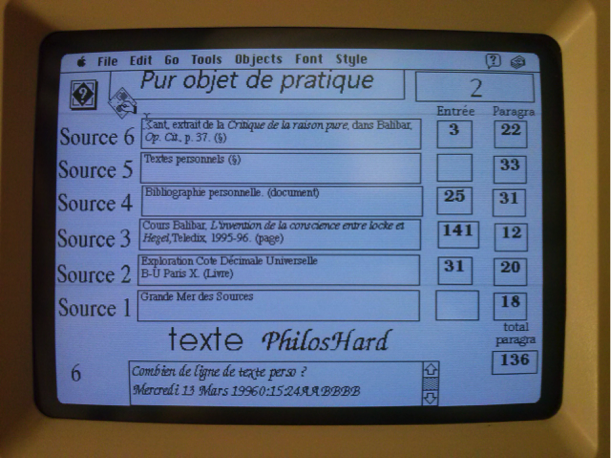
\includegraphics{media/1000000100000263000001CB6B57709BAD5234C1.png}

}

\caption{\label{fig-appliHypercard}Application Hypercard pour la
génération automatique de textes philosophiques}

\end{figure}%

Curieux d'explorer plus précisément cette intuition, je me lance dans
une thèse grâce à ma rencontre avec
\href{http://localhost/samszo/omk/s/fiches/item/61153}{Jean-Pierre
Balpe} et \href{http://localhost/samszo/omk/s/fiches/item/61148}{Imad
Saleh} qui m'encouragent à travailler sur la conception d'agents
autonomes pour générer des hypertextes adaptatifs. Trop autonome, je ne
réalise pas à l'époque l'importance de travailler collectivement dans un
laboratoire de recherche, je parts en voyage et mène mes recherches de
manière solitaire jusqu'à ce que dix ans plus tard je retrouve
Jean-Pierre et Imad. Fort de nouvelles expériences comme consultant
spécialiste en système d'information et en développement Web
(cf.~\href{http://localhost/samszo/omk/s/fiches/item/300719}{Carrière
privée}), je reviens à l'université pour cette fois participer
activement à la vie du
\href{http://localhost/samszo/omk/s/fiches/item/299601}{laboratoire
Paragraphe}, tout d'abord comme conférencier puis chargé de cours et
professeur contractuel. L'opportunité d'un contrat doctoral me permet de
mener à bien une thèse sous la direction
d'\href{http://localhost/samszo/omk/s/fiches/item/61148}{Imad Saleh} et
de m'inscrire pleinement dans une
\href{http://localhost/samszo/omk/s/fiches/item/300716}{carrière
universitaire} que je mène comme Maître de conférence en science de
l'information et de la communication depuis 2013.

L'atmosphère très fertile au sein de Paragraphe et les relations
intenses que ce laboratoire entretient avec la communauté des sciences
de l'information et de la communication, a stimulé l'engagement de mes
recherches dans de multiples collaborations en France et à l'étranger
Figure~\ref{fig-collabMondeSamszo}. Celles-ci m'ont permis de découvrir
des milieux et des pratiques très diverses, par exemple en collaborant
avec des institutions prestigieuses comme la Bibliothèque Nationale de
France, les Archives Nationales ou l'INA, avec des programmes de
recherche ANR comme Biolographes ou Aliento, avec des projets de
recherches internationaux comme Arcanes, avec des groupes de recherches
comme GENIC ou MANEP, avec des enjeux sociétaux importants comme celui
de l'accessibilité, de l'écologie ou de l'éthique.

La participation dès l'origine à trois Projets d'Investissement d'Avenir
(PIA) que sont le laboratoire d'excellence H2H, l'IDEFI CréaTIC et l'EUR
ArTec, m'a donné la chance de découvrir des projets importants tout à la
fois en terme de gouvernance de la recherche que de possibilité
d'expérimentation. De même, mon implication dans les instances de
l'Université Paris 8 en tant que membre du Conseil Documentaire du SCD,
du conseil pédagogique de l'UFR STN et de la commission de spécialistes
en Science de l'Information et de la Communication, me donne une bonne
connaissance des rouages nécessaires et des difficultés qu'il faut
surmonter pour que les activités de recherche et la vie des institutions
se développent.

Grâce à ces activités, j'ai eu la chance de dialoguer avec de très
nombreux chercheurs dont la liste complète serait trop longue à faire
figurer ici mais que je remercie vivement pour ces conversations où
l'échange de points de vue parfois très différents donnent à la
recherche un goût à la fois subtile, surprenant et aventureux. Une
première vision de ces relations est visible dans le diagramme
ci-dessous qui montre l'évolution de mes productions scientifiques
déposé dans HAL suivant deux catégories : celle des mots clefs utilisés
pour décrire ces dépôts et celle des collaborateurs ayant participé à la
production :

\begin{figure}

\centering{

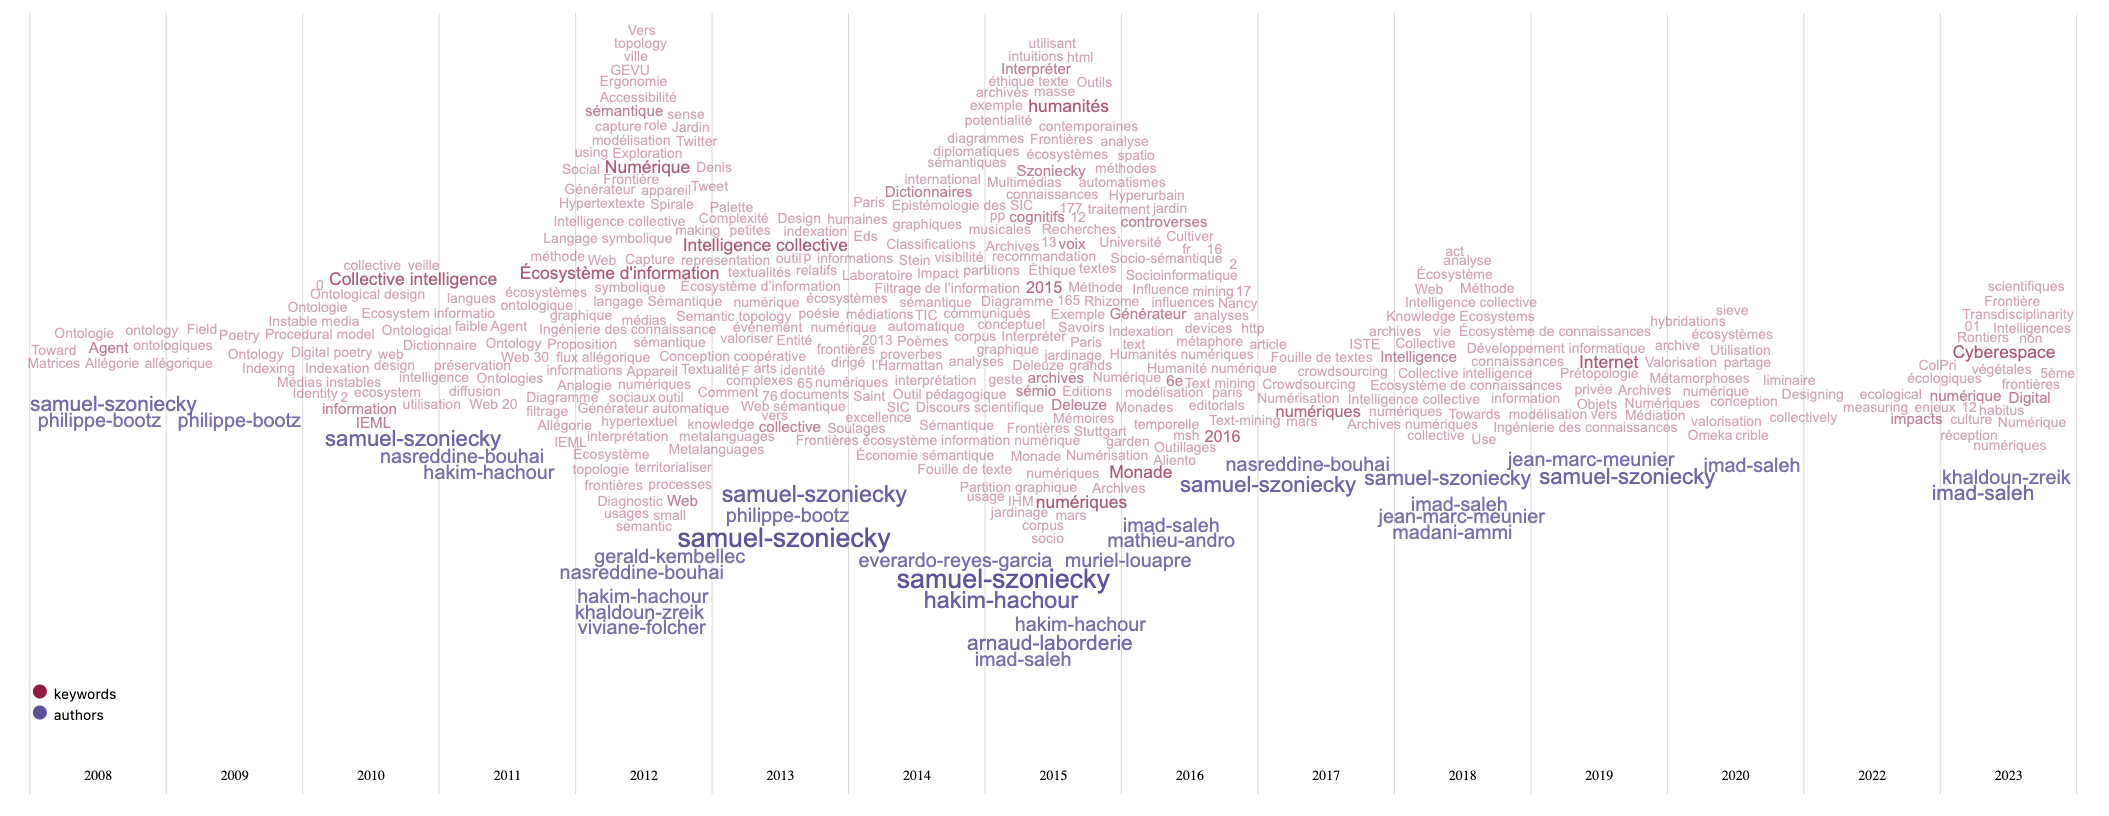
\includegraphics{images/steamHALsamszo.png}

}

\caption{\label{fig-steamHalSamszo}Evolution des productions}

\end{figure}%

On le voit, l'essentiel des productions se font avec des collègues du
Laboratoire Paragraphe notamment à cause des proximités géographiques
mais aussi grâce aux affinités intellectuelles et aux perspectives
communes. Toutefois, ce graphique est l'arbre qui cache une forêt
beaucoup plus dense car il ne montre pas les relations que j'entretiens
avec les collègues avec qui je partage des évènements scientifiques. De
même concernant l'évolution des concepts en lien avec mes productions
qui dans ce diagramme ne présente qu'une toute petite partie du paysage
sémantique que j'explore. Je vous propose d'appronfondir cette
exploration en explicitant mon parcours à travers quelques exemple de
publications puis en analysant ce paysage à partir de ma veille
informationnelle.

\section{Mon parcours en Sciences de l'information et de la
communication}\label{sec-posiSIC}

Les sciences de l'information et de la communication ont pour but entre
autres de concevoir, expérimenter et critiquer des modèles conceptuels
permettant de quantifier l'information et de qualifier la communication.
Ce double aspect des SIC est sans doute caricatural mais il pose à mon
sens les deux pôles entre lesquels cette discipline est en tension. D'un
coté nous avons dans la continuation de Shannon, Weaver et des
technologies de l'information, une recherche sur les moyens de modéliser
l'information pour fournir la matière nécessaire au développement de
technologies stables. De l'autre coté, en relation avec les sciences
humaines, nous avons dans la continuation des études en communication,
une recherche sur l'analyse des pratiques d'échanges. Nous développons
ces deux pôles des SIC dans nos enseignements et dans nos recherches.

Mon travail de thèse a été l'occasion de théoriser mes intuitions sur
l'utilité de l'informatique et des langages formels pour le travail
collectif en sciences humaines et plus spécifiquement dans les sciences
de l'information et de la communication. A partir de cette thèse, des
ouvrages et des articles qui ont suivis, j'ai élaboré une méthode
générique pour la modélisation onto-éthique des écosystèmes de
connaissances. Cette méthode s'articule autour d'un diagramme
représentant quatre dimensions existentiels~: matérielles
Section~\ref{sec-espaceMateriels}, sociales
Section~\ref{sec-espaceActant}, conceptuelles
Section~\ref{sec-espaceConceptuels} et rapports
Section~\ref{sec-rapportsInstExis}. L'objectif est d'utiliser ce
diagramme pour modéliser des «~manières d'être~» dans un espace-temps
spécifique ou pour dire autrement de décrire un point de vue spécifique
et ces évolutions dans un écosystème de connaissances.

Cette méthode de modélisation et d'analyse de l'information et de la
communication est mise en pratique dans des cours et des projets de
recherche. Les objectifs pédagogiques principaux de ces cours sont~:

\begin{itemize}
\item
  comprendre les principes de complexité,
\item
  abandonner la démarche d'exhaustivité au profit des choix nécessaires
  à la problématisation,
\item
  dépasser la difficulté de choisir le statut de l'information,
\item
  respecter des contraintes formelles par soucis d'interopérabilité.
\end{itemize}

Plusieurs projets de recherche m'ont permis d'expérimenter cette méthode
pour laquelle j'ai conçu et développé des prototypes informatiques
spécifiques. Ces expériences me sont très utiles pour évaluer en quoi la
méthode est générique, compréhensible et utilisable
\textbf{?@sec-part-technoIntello}.

De ces expérimentations un programme de recherche se dégage qui vise
plusieurs objectifs. Premièrement diffuser le modèle onto-éthique en
publiant des recueil de diagrammes composés dans les cours et les
projets de recherche. Parallèlement, les applications développées pour
la modélisation seront documentées et le code mis à disposition de la
communauté des chercheurs et des développeurs. Le modèle sera aussi
diffusé dans un séminaire de recherche sur la modélisation des
connaissances en sciences humaines, ouvert aux chercheurs réalisant un
corpus numériques et désirant employer des méthodes d'Humanités
Numériques innovantes. L'objectif est d'accompagner les chercheurs pour
modéliser des recherches en humanités numériques en diffusant des bonnes
pratiques et des outils efficaces. Deuxièmement, développer des outils
intellectuels pour cartographier les connaissances en concevant des
interfaces simples et modulaires pour~:

\begin{itemize}
\item
  calculer la complexité de points de vue,
\item
  cartographier le flux d'information et de communication,
\item
  modéliser graphiquement une existence informationnelle dans un
  écosystème de connaissances,
\item
  stimuler des explorations cognitives en générant des frayages
  intellectuels,
\item
  recommander des conversations créatrices.
\end{itemize}

Pour illustrer cette démarche nous présentons ci-dessous un résumé des
publications et des projets qui nous semble les plus représentatifs de
notre parcours.

\subsection{Écosystème de connaissances, méthode de modélisation et
d'analyse de l'information et de la
communication}\label{uxe9cosystuxe8me-de-connaissances-muxe9thode-de-moduxe9lisation-et-danalyse-de-linformation-et-de-la-communication}

A destination des étudiants de Master, cet ouvrage(Szoniecky, 2017)
présente les principes de base de la méthode que j'ai conçu pour
modéliser et analyser l'information et la communication. J'y présente
dans une première partie l'intérêt de concevoir l'information et la
communication en tant qu'écosystème et les principes fondamentaux de
modélisation qu'on en déduit. La deuxième partie est une mise en
pratique des principes théorique à travers des exemples concret d'usages
de la méthode.

\subsection{Métamorphoses et hybridations d'une archive numérique pour
sa valorisation: Vers des écosystèmes de
connaissances}\label{muxe9tamorphoses-et-hybridations-dune-archive-numuxe9rique-pour-sa-valorisation-vers-des-uxe9cosystuxe8mes-de-connaissances}

Cet article (Szoniecky, 2019) présente un projet de recherche mené dans
le cadre d'un atelier laboratoire CreaTIC pour expérimenter le
développement d'une intelligence collective entre les étudiants de
l'université Paris 8 et les millions de documents conservés dans les
bâtiments de Archives Nationales. L'article montre comment décrire un
processus de numérisation en terme de métamorphose et d'hybridation d'un
écosystème de connaissance. Il présente des outils pour un «~culture
intensif~» de l'information et un prototype développé dans le cadre de
ce projet pour «~le jardinage collectif des connaissances~».

\subsection{Espace liminaire de l'authenticité: Une démarche d'humanités
numériques}\label{espace-liminaire-de-lauthenticituxe9-une-duxe9marche-dhumanituxe9s-numuxe9riques}

L'activité automatisée de production de faux, tels que les
\hspace{0pt}fake news\hspace{0pt} et le
\hspace{0pt}deepfake\hspace{0pt}, engendre des répercussions dans
l'espace social tangible et concernent les relations de confiance que
nous construisons quotidiennement avec l'information qui nous parvient.
Cet article (Bourassa et al., 2019) traite de la transformation de
l'espace de médiation et cherche à comprendre la redéfinition actuelle
et futures des notions d'authenticité et d'autorité liées à l'accord de
la légitimité. Il porte aussi sur le dialogue performatif des données et
des actions collectives d'utilisateurs.

\subsection{Knowledge Design in the Internet of Things : Blockchain and
Connected
Refrigerator}\label{knowledge-design-in-the-internet-of-things-blockchain-and-connected-refrigerator}

L'Internet des objets fait partie de notre vie quotidienne, mais de
nombreux utilisateurs ne comprennent pas les relations de ces objets
avec les réseaux numériques, ni les données qui transitent à partir des
usages qu'ils en font. Dans cet article (Szoniecky \& Toumia, 2019),
nous supposons que les représentations dynamiques et interactives du
pouvoir d'action des utilisateurs et des objets sont des moyens de mieux
comprendre de quoi ces dispositifs sont capables. Pour ce faire, nous
concevons une conception sécurisée et respectueuse de la vie privée des
connaissances dans l'environnement des objets connectés. Nous analysons
l'exemple d'un réfrigérateur connecté pour comprendre comment utiliser
la Blockchain pour développer des Innovations Sociales Numériques.

\subsection{Conception d'un crible pour mesurer collectivement les
impacts écologiques de
l'activité}\label{conception-dun-crible-pour-mesurer-collectivement-les-impacts-uxe9cologiques-de-lactivituxe9}

Cet article (Szoniecky, 2020) présente une méthode pour concevoir un
dispositif générique de métrologie citoyenne que nous appelons crible et
dont nous étudions la conception dans le contexte de l'écologie de
l'activité, plus précisément dans l'exemple de la consommation d'avocat.
Cette conception s'appuie sur une modélisation éthique de l'activité
faisant référence à {[}Guattari (1989); G. Deleuze (1988); µ et al.
(2015a); Citton (2008b){]}(Berque, 2009a; Philippe. Descola, 2005) et
s'appuyant sur les exigences qu'une telle démarche implique pour la
gestion des données. Le crible en tant qu'interface entre objectivité et
subjectivité offre une analogie opératoire pour explorer les
conséquences de l'activité à partir d'un modèle simple d'écriture et de
lecture basée sur la formule logique sujet -- objet - prédicat
contrainte par l'ontologie éthique~: physicalités, acteurs, concepts,
rapports.

\subsection{Projet LITTE\_BOT}\label{sec-projetLitteBot}

Le projet LITTE\_BOT (Pappa et al., 2023; Quach et al., 2022) consiste
en la création d'un chatbot théâtral incarnant Dom Juan à l'occasion du
400ème anniversaire de la naissance de Molière, présenté pour
l'exposition ``Molière, le jeu du vrai et du faux'' que lui ont
consacrée la BnF et la Comédie Française. fin 2022. A l'origine de ce
projet, Rocio Berenguer, une dramaturge, s'est rapprochée de la BnF pour
récupérer un corpus pour créer un chatbot littéraire. Le projet Gallica
Studio, aujourd'hui terminé, encourageait la réutilisation des contenus
de Gallica, dont la plupart sont dans le domaine public, tout en
invitant à l'expérimentation de nouveaux usages rendus possibles par les
technologies émergentes. En l'occurrence, explorer la médiation vocale
rendue possible par les chatbots et expliquer cette technologie au grand
public. En collaboration avec Anna Pappa, nous avons apporté notre
expertise scientifique pour faire du chatbot une réalité, dans le cadre
d'un appel à projets de l'EUR Artec.

L'objectif était de créer un chatbot ouvert capable d'incarner le Dom
Juan de Molière. Le défi technique était de créer une base de données
suffisamment grande pour entraîner le modèle de langage séquence à
séquence. Les modèles linguistiques actuels sont formés avec des corpus
contemporains. Pour notre projet, nous devions construire de toutes
pièces une base de données qui permettrait à une intelligence
artificielle d'imiter le Dom Juan de Molière, de parler le français du
XVIIe siècle et de comprendre le français actuel parlé par son
interlocuteur.

La base de données pour la formation du chatbot est non seulement
indispensable, mais aussi la partie la plus importante de ce projet.
Dans un premier temps, j'ai travaillé sur l'analyse sémantique du corpus
Molière disponible sur Gallica grâce à un précédent partenariat de
recherche entre la BnF et le laboratoire OBVIL de la Sorbonne. La mise à
disposition de ce corpus des textes de Molière dans un format
manipulable par des machines
(\url{https://obvil.sorbonne-universite.fr/corpus/moliere/moliere})
permet d'envisager de multiple réutilisation de ces textes pour des
usages innovants. Par exemple, l'Obvil analyse les relations entre les
personnages d'une pièce de théâtre pour visualiser l'importance de leurs
relations :

\begin{figure}

{\centering 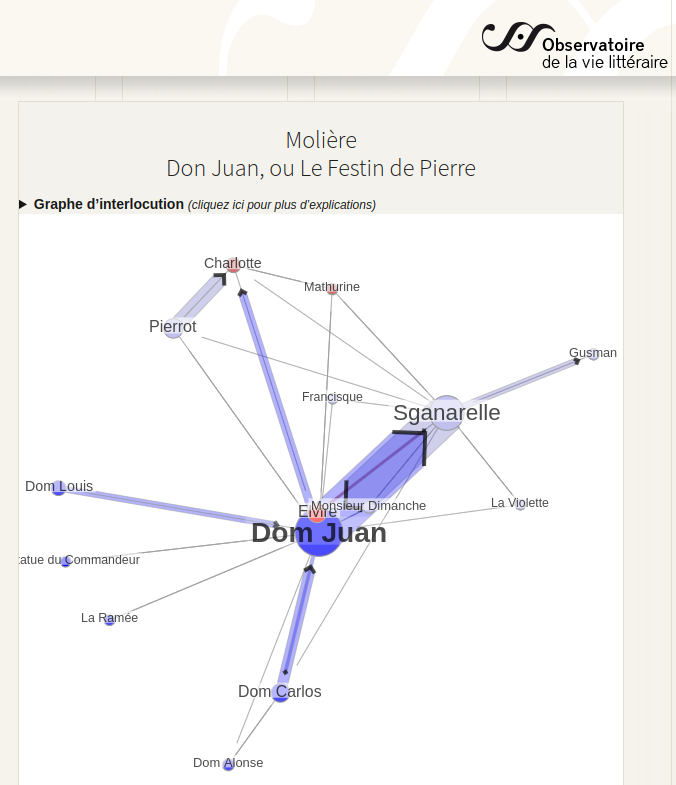
\includegraphics{images/obvil_corpus_moliere_moliere_dom-juan-1682.png}

}

\caption{Obvil : représentation des relations entre personnages}

\end{figure}%

Pour ce projet nous avons analysé la structure du corpus (pièces de
théâtre, actes, scènes, répliques, phrases, mots-clés) pour créer des
éléments dans une base de données Omeka S correspondant à chacune de ces
structures et à leurs relations. Pour ce faire nous avons développé un
module générique \footnote{Lien vers les sources du module :
  \url{https://github.com/samszo/Omeka-S-module-Scraping}} d'importation
des pages HTML qui à partir d'un fichier de configuration\footnote{lien
  vers le fichier de configuration pour l'importation des pièces de
  Molière :
  \url{https://github.com/samszo/Omeka-S-module-Scraping/blob/main/data/exemples/moliereParPiece.json}}
sélectionne les éléments de la page et les enregistre dans la base Omeka
S en détaillant leurs relations. Nous avons importer toutes \footnote{Lien
  vers les pièces importées
  :\url{http://localhost/omk_moliere/s/theatre-de-moliere/item?resource_class_id\%5B\%5D=1017&sort_by=created&sort_order=desc&submit=Search}}
pour obtenir une base de plus de 100 000 items. Ce travail
d'hypertrextualisation permet d'explorer la base de données et
d'enrichir les éléments qui la compose et dont voici la représentation :

Nous souhaitions travailler précisément les répliques du théâtre de
Molière afin de les rendre génératives en suivant le modèle des
générateurs de Jean Pierre Balpe Section~\ref{sec-ateliersGenerateur}.
et ainsi disposé d'un générateur automatique de répliques de Molière
pouvant servir à l'entrainement du chatbot. Malheureusement, nous
n'avons pas trouvé les ressources nécessaires pour faire ce travail en
détail. Nous avons privilégié une approche plus rapide en indexant
manuellement les répliques selon des étiquettes correspondant au
scénario suivi par le chatbot. En réalité, LITTE\_BOT combine deux
chatbots : un chatbot ouvert basé sur le modèle Seq2Seq et un chatbot
scénarisé, aux lignes indexées.

Cette pratique de la scénarisation des chabots reste aujourd'hui la plus
répandue car elle permet de maîtriser précisément le processus de
dialogue entre les utilisateurs et les bots. Comme le confirme les
indexations manuelles par micro-tâches faites pour rendre ChatGPT
opérationnel ou le chatbot Chomsky VS Comsky

\subsection[Projet Polemika]{\texorpdfstring{Projet
Polemika\footnote{Ce paragraphe est issu du rapport final du projet}}{Projet Polemika}}\label{projet-polemikapositionnements-6}

Polemika a été financé par les Trophées franciliens de l'innovation
numérique dans le supérieur (Trophées EdTech) et l'EUR ARTeC (Ecole
Universitaire de Recherche). Ce projet visait à développer un générateur
automatique d'arguments pour l'éducation à l'esprit critique. S'appuyant
sur des travaux menés au laboratoire Paragraphe (Balpe, 2002; Szoniecky,
Balpe, \& Reyes, n.d.; Szoniecky, Hachour, \& Bouhai, 2012) sur un
générateur automatique de texte, nous disposions d'une infrastructure
pré-existante, pour la génération automatique de structures textuelles.
Partant du constat de la généralisation du phénomène des fake news, et
dans le contexte numérique Polemika vise à générer des contre-arguments
mais aussi de l'absurde, des caricatures, des exagérations, voire des
fake news, afin de travailler les compétences d'esprit critique par la
pratique, de manière ludique et interactive. Une des hypothèses consiste
à observer si à travers la répétition de la mise en œuvre d'opérations
de prise de distance, de prise de recul lors de la confrontation
itérative à des énoncés plausibles, mais faux, ou à des énoncés absurdes
ou caricaturaux, générés par Polemika, on parviendrait à augmenter la
qualité des critiques réalisées sur les énoncés, mais également à
diminuer l'impact émotionnel, à travers un processus « d'habituation »
et d'éducation, qui vise à porter les publics à aller vérifier
l'information plutôt que de commencer par réagir émotionnellement.

Ce projet est à la croisée interdisciplinaire de plusieurs champs de
recherche et d'expertises : pédagogie et sciences de l'éducation,
psychologie, informatique et sciences de l'information. Nous l'avons
donc mené avec des chercheurs de ces différentes spécialités mais le
fondement disciplinaire s'inscrit en SIC notamment parce que les travaux
sur l'EMI, l'Information Literacy et l'esprit critique sont bien ancrés
en SIC. Parmi les dispositifs d'éducation à la pensée critique, les jeux
sérieux tiennent une place particulière du fait de la possibilité de
toucher un nombre important d'individus et, grâce à la dimension ludique
de les fidéliser et ainsi d'engager les participants dans l'acquisition
de compétences approfondies. On peut distinguer deux grandes approches.
La première consiste à confronter les participants à des fake news en
leur apprenant à identifier les critères pertinents de détection des
fake news en évaluant notamment la source et la cohérence du contenu. Ce
type d'approche s'avère insuffisant car (1) la répétition de fake news
favorise un sentiment de familiarité qui à son tour augmente la
crédibilité; (2) les corrections sont souvent inefficaces car les gens
continuent à se fier à leur première évaluation notamment parce que le
registre de la contre argumentation n'est pas le même que celui sur
lequel la conviction a été construite. La seconde approche s'appuie sur
l'analogie biologique de ``l'inoculation''. Elle consiste à enseigner
aux participants à faire des fake news pour renforcer la résilience face
à celles-ci. Par exemple, le jeu FakeYou entraîne les joueurs à générer
leurs propres faux titres et ainsi les familiariser avec les procédés de
formulation de fake news convaincantes. Leurs résultats montrent une
diminution de la sensibilité (habituation) aux fake news, mais montrent
également que les utilisateurs privilégient des procédés spécifiques
pour générer des fausses nouvelles. De notre point de vue, ce n'est pas
la création, mais la plus grande implication des sujets qui explique la
diminution de la sensibilité aux fake news. Notre proposition est à
mi-chemin de ces deux approches. Il ne s'agit cependant pas d'une simple
exposition à des fake news puisque dans ce projet les joueurs pourront
``dialoguer'' avec le dispositif, lequel pourra jouer sur les niveaux
émotionnels et les mondes sociaux développés. Nous avons mené à bien ce
qui pouvait l'être dans les conditions du Covid. Tout le volet
expérimental en présentiel et événementiel a dû être annulé.

\subsubsection{Prototypes réalisé pour
Polemika}\label{prototypes-ruxe9alisuxe9-pour-polemika}

Dans le cadre de ce projet nous avons conçu et développé plusieurs
prototypes afin d'expérimenter nos hypothèses. Le diagramme ci-dessous
montre l'écosystème de connaissances que nous avons conçu pour le
développement des prototypes.

\begin{figure}

\centering{

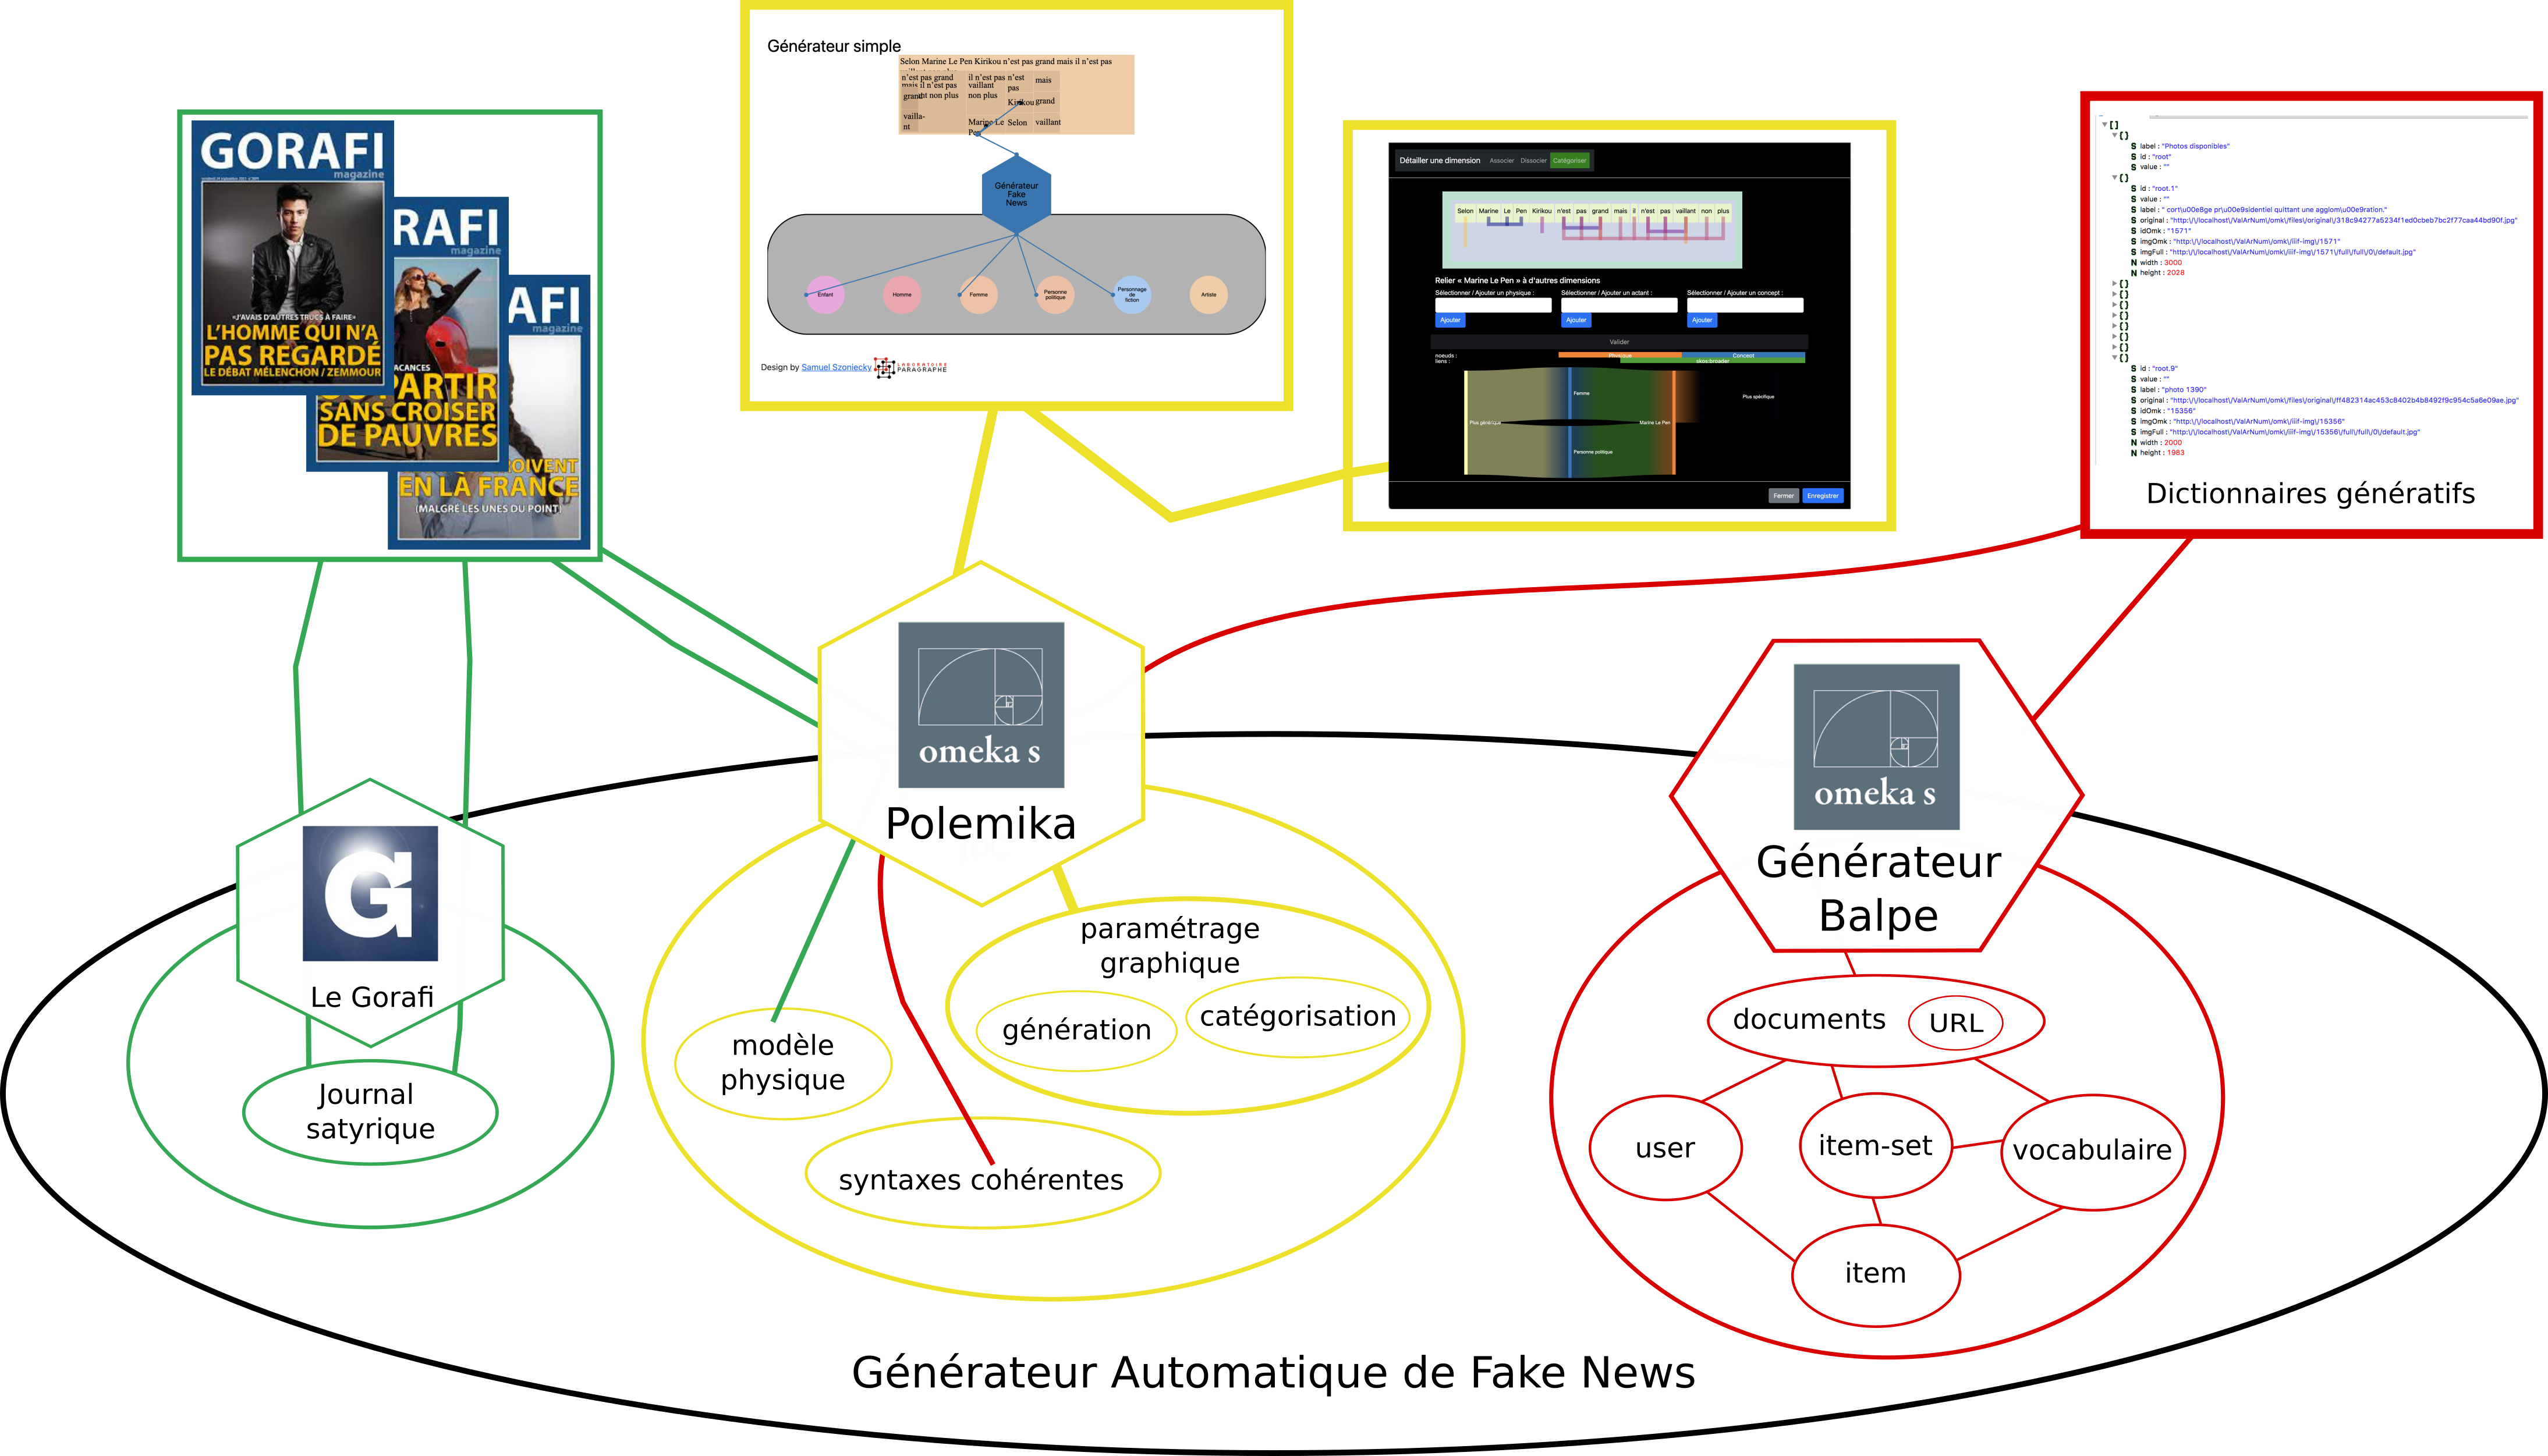
\includegraphics{images/ice_generateur.png}

}

\caption{\label{fig-iceGenerateurPolemika}Ecosystème de génération
automatique de Fake News}

\end{figure}%

\paragraph{Générateur automatique de
texte}\label{guxe9nuxe9rateur-automatique-de-texte}

Sur la base des travaux menés avec Jean-Pierre Balpe sur les générateurs
automatiques de texte, nous avons développé une nouvelle version du
générateur qui utilise Omeka S comme système de gestion des données en
intégrant l'interopérabilité sémantique du Linked Open Data (LOD) et des
modules spécifiques pour la manipulation et le paramétrage des
algorithmes génératifs.

\subparagraph{Première version :
GenLOD}\label{premiuxe8re-version-genlod}

Cette première version reprend intégralement les principes des
générateurs balpiens notamment les dictionnaires de concepts (494838
items) et les algorithmes de cohérence des syntaxes. Cette version a été
développée sous la forme d'un module Omeka S en collaboration avec
Daniel Berthereau. Les données disponibles sont consultable ici :
https://jardindesconnaissances.univ-paris8.fr/genlod/omk/s/donnees-disponibles/item
. Le code source est accessible ici :
https://github.com/samszo/omeka-s-module-generateur .

\begin{figure}

\centering{

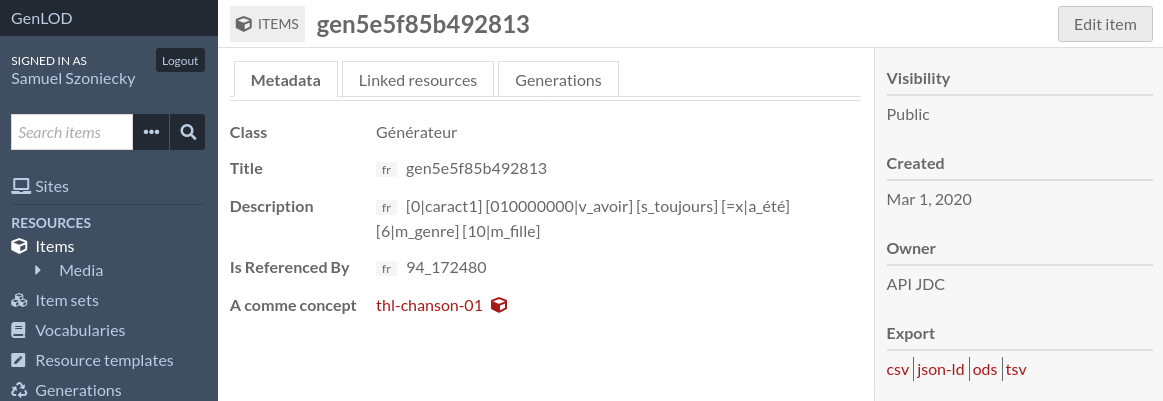
\includegraphics{images/GenLodOmk.png}

}

\caption{\label{fig-GenLOGomk}Exemple de générateur balpien}

\end{figure}%

Outre les générateurs balpiens, GenLOD met à disposition de nouveaux
types de générateurs.

\begin{itemize}
\tightlist
\item
  Générateur SPARQL
\end{itemize}

Ce générateur utilise les capacités des requêtes SPARQL pour récupérer
des données aléatoires sur un sujet très précis dans les bases de
données du LOD.

\begin{figure}

\centering{

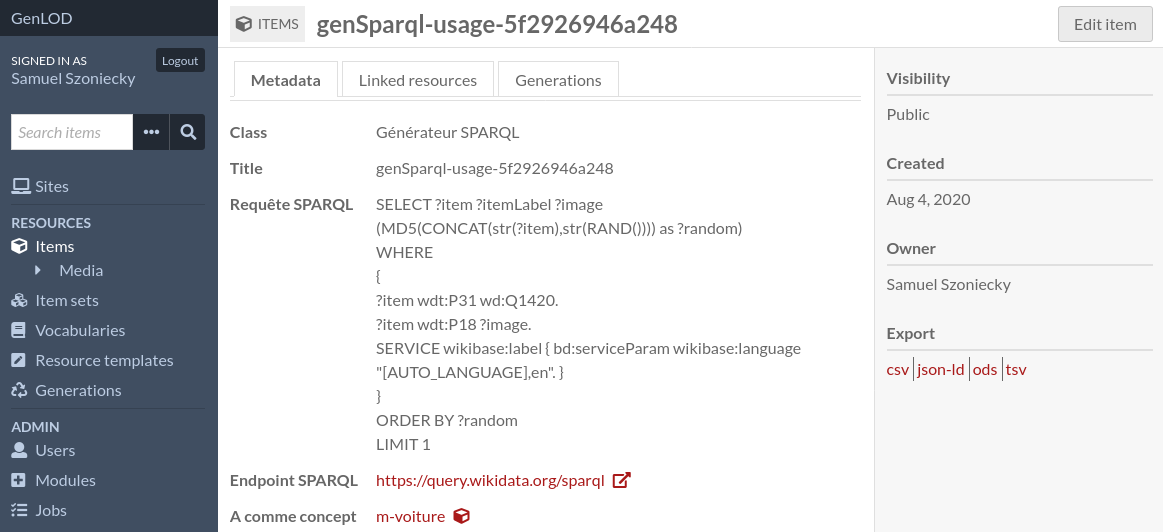
\includegraphics{images/GenLodOmkSPARQL.png}

}

\caption{\label{fig-GenLOGomkSparql}exemple de générateur SPARQL}

\end{figure}%

\begin{itemize}
\tightlist
\item
  Générateur IEML
\end{itemize}

Ce générateur utilise les capacités génératives du langage d'adressage
des concepts IEML pour obtenir des données liée sémantiquement avec un
concept donnée.
https://pierrelevyblog.com/2021/09/20/pour-un-changement-de-paradigme-en-intelligence-artificielle/

\begin{itemize}
\tightlist
\item
  Générateur Wikidata
\end{itemize}

Ce générateur utilise un lien sémantique avec les données de Wikidata
pour alimenter le générateur avec données liées.

\begin{itemize}
\tightlist
\item
  Générateur Synonyme
\end{itemize}

Ce générateur utilise la base de données de synonyme et d'antonyme mis à
disposition par le Crisco pour augmenter les capacités génératives des
concept tout en conservant une cohérence sémantique.
https://crisco2.unicaen.fr/des/

\begin{figure}

\centering{

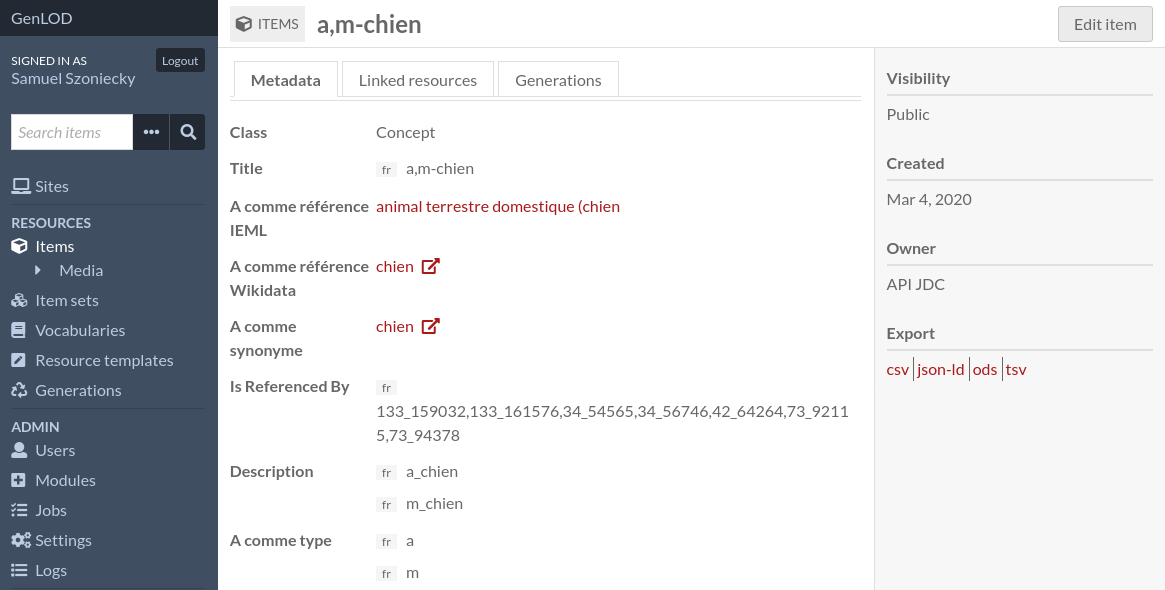
\includegraphics{images/GenLodOmkIEML.png}

}

\caption{\label{fig-GenLOGieml}Exemple de générateur IEML, Wikidata,
Synonyme}

\end{figure}%

Le générateur GenLOD est encore un prototype dont il faut améliorer les
performances et l'ergonomie de ses usages. Toutefois, il nous a permis
de poser les principes fondamentaux d'un générateur utilisant les
fonctionnalité du Web sémantique et du LOD.

\subparagraph{Deuxième version : jardin des
connaissances}\label{deuxiuxe8me-version-jardin-des-connaissances}

La deuxième version du générateur automatique de texte utilise les
principes des écosystèmes de connaissance pour concevoir une interface
graphique de jardinage de l'information afin d'améliorer les
performances et l'ergonomie du prototype GenLOD. Il a été développé sous
la forme d'un module Omeka S :
https://github.com/samszo/Omeka-S-module-JDC

\begin{figure}

\centering{

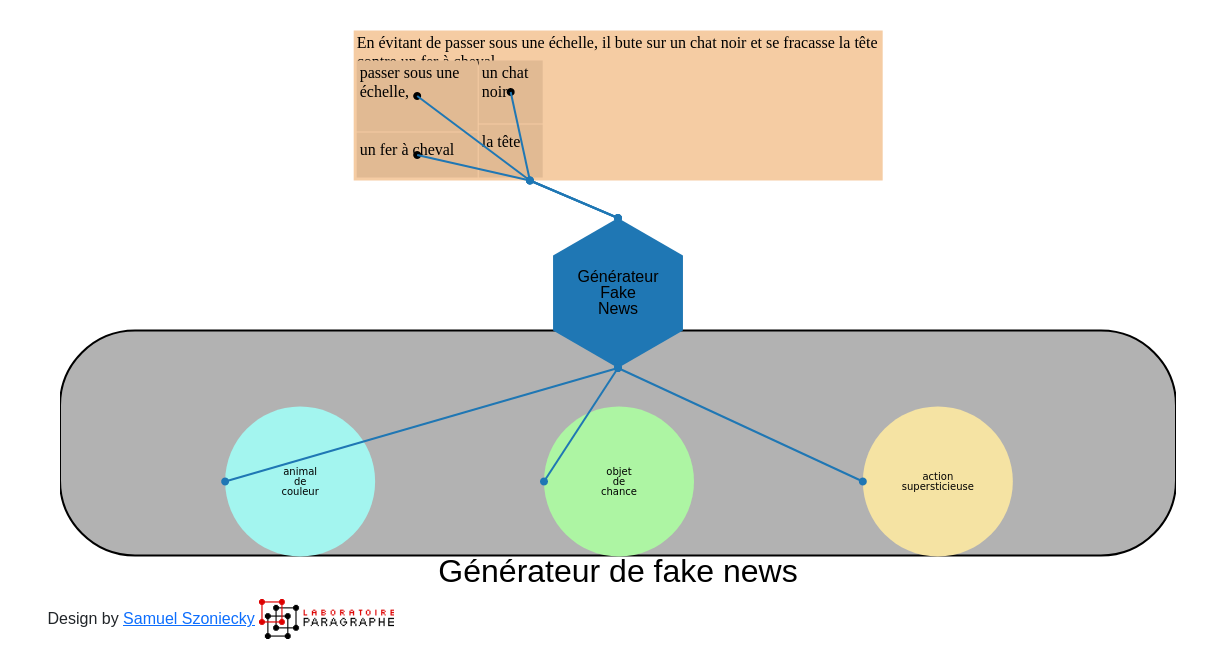
\includegraphics{images/GenJDC.png}

}

\caption{\label{fig-GenJDC}Générateur de fake news sous forme
d'écosystème à jardiner}

\end{figure}%

Ce générateur toujours à l'état de prototype semble être une voie
prometteuse pour rendre accessible à un plus grand public l'utilisation
des générateurs.

\paragraph{Interface de cartographie des
arguments}\label{interface-de-cartographie-des-arguments}

Afin de paramètrer le plus finement possible les générateurs à partir de
nos hypothèses de recherches, nous avons conçu et développé des outils
pour la cartographie des arguments.

\subparagraph{Visualisation CMap dans Omeka
S}\label{visualisation-cmap-dans-omeka-s}

Le premier prototype que nous avons réalisé se base sur nos pratiques
d'un outils de cartographie conceptuelle : CMAP Tools
https://cmap.ihmc.us/ Nous utilisons cette outils pour rapidement
construire des cartes conceptuelles et les mettre à disposition des
collègues et des étudiants. Toutefois, il ne permettais pas une
intégration fine avec les données stockées dans Omeka S. Nous avons donc
développé : - un module pour importer les données des cartes sémantique
CMAP dans Omeka S afin de travailler plus finement les concepts présents
dans la carte notamment en les mettant en relation avec les différents
générateurs développés. Le code du module est accessible ici :
https://github.com/samszo/Omeka-S-module-CmapImport - une interface de
visualisation des cartes à partir des données importées :

\begin{figure}

\centering{

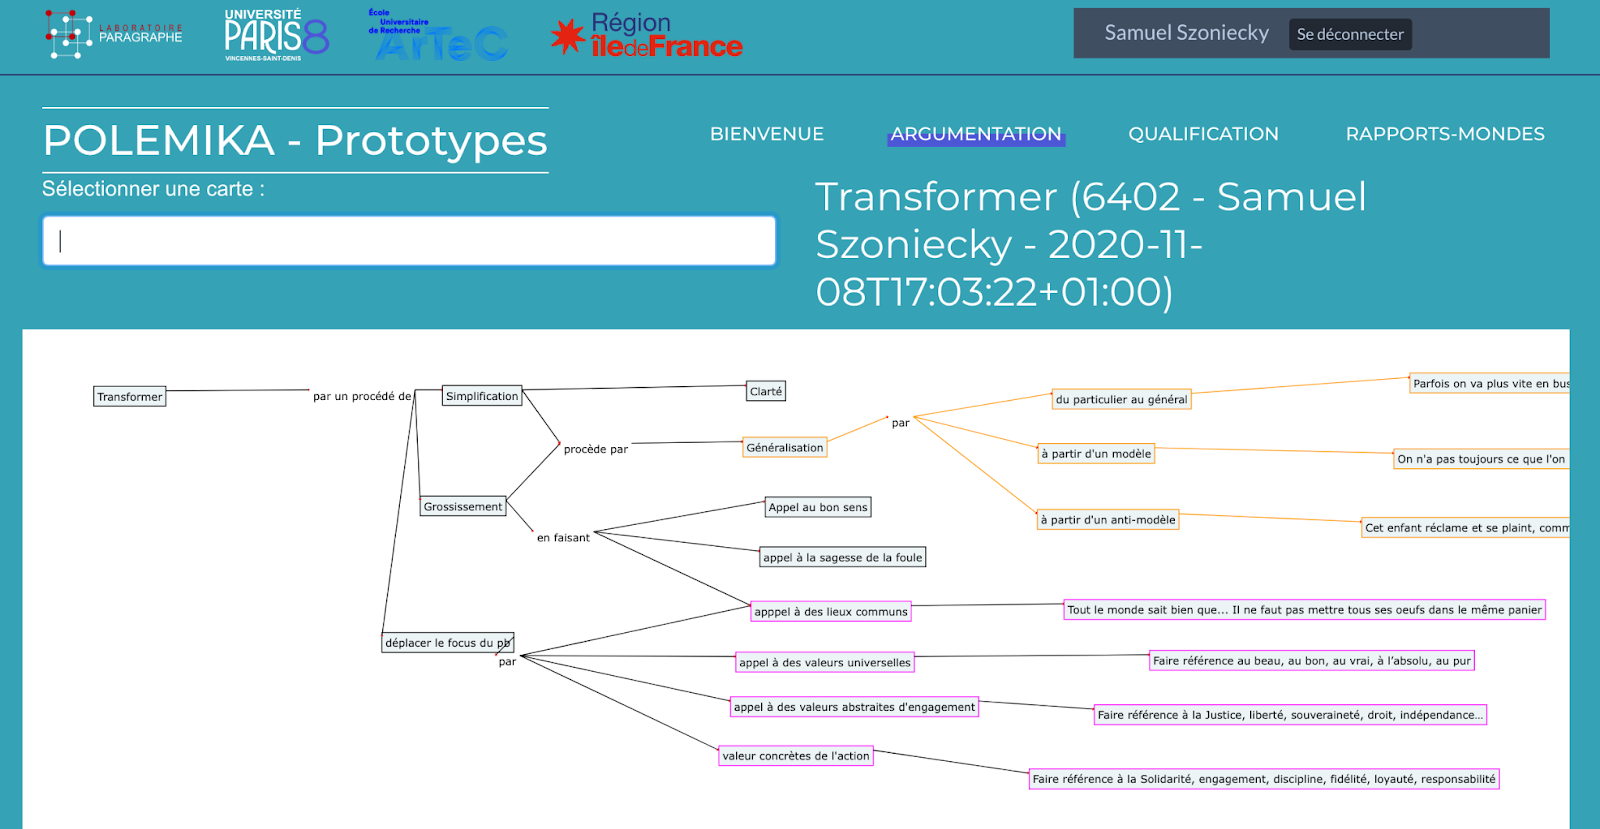
\includegraphics{images/polemikaCMAP.png}

}

\caption{\label{fig-polemikaCMAP}Visualisation d'une carte CMAP dans
Omeka S}

\end{figure}%

Cette première version nous a montré l'importance de ce type d'outils
pour la suite du projet nous avons donc décidé de développé une version
plus dynamique et intéractive de l'interface de consultation des cartes
conceptuelles.

\subparagraph{Editeur de cartographie
sémantique}\label{editeur-de-cartographie-suxe9mantique}

Cette éditeur de cartographies conceptuelles fonctionne à partir des
données provenant d'une carte CMAP mais aussi de manière autonome. Il
permet de gérer graphiquement la lecture, l'écriture, et la mise à jour
des cartes à la fois dans le positionnement des éléments la constituant,
le style de chaque élément à partir d'archétypes graphiques,
l'enrichissement des concepts directement dans la base de données Omeka
S. L'éditeur est composé : - d'un thème Omeka S accessible ici :
https://github.com/samszo/Omeka-S-theme-PolemikaProto - d'un module
Omeka S de cartographie des affects accessible ici :
https://github.com/samszo/Omeka-S-module-CartoAffect - d'un l'éditeur
graphique utilisable ici :
https://polemika.univ-paris8.fr/omk/s/seconds-prototypes/page/editeur

\begin{figure}

\centering{

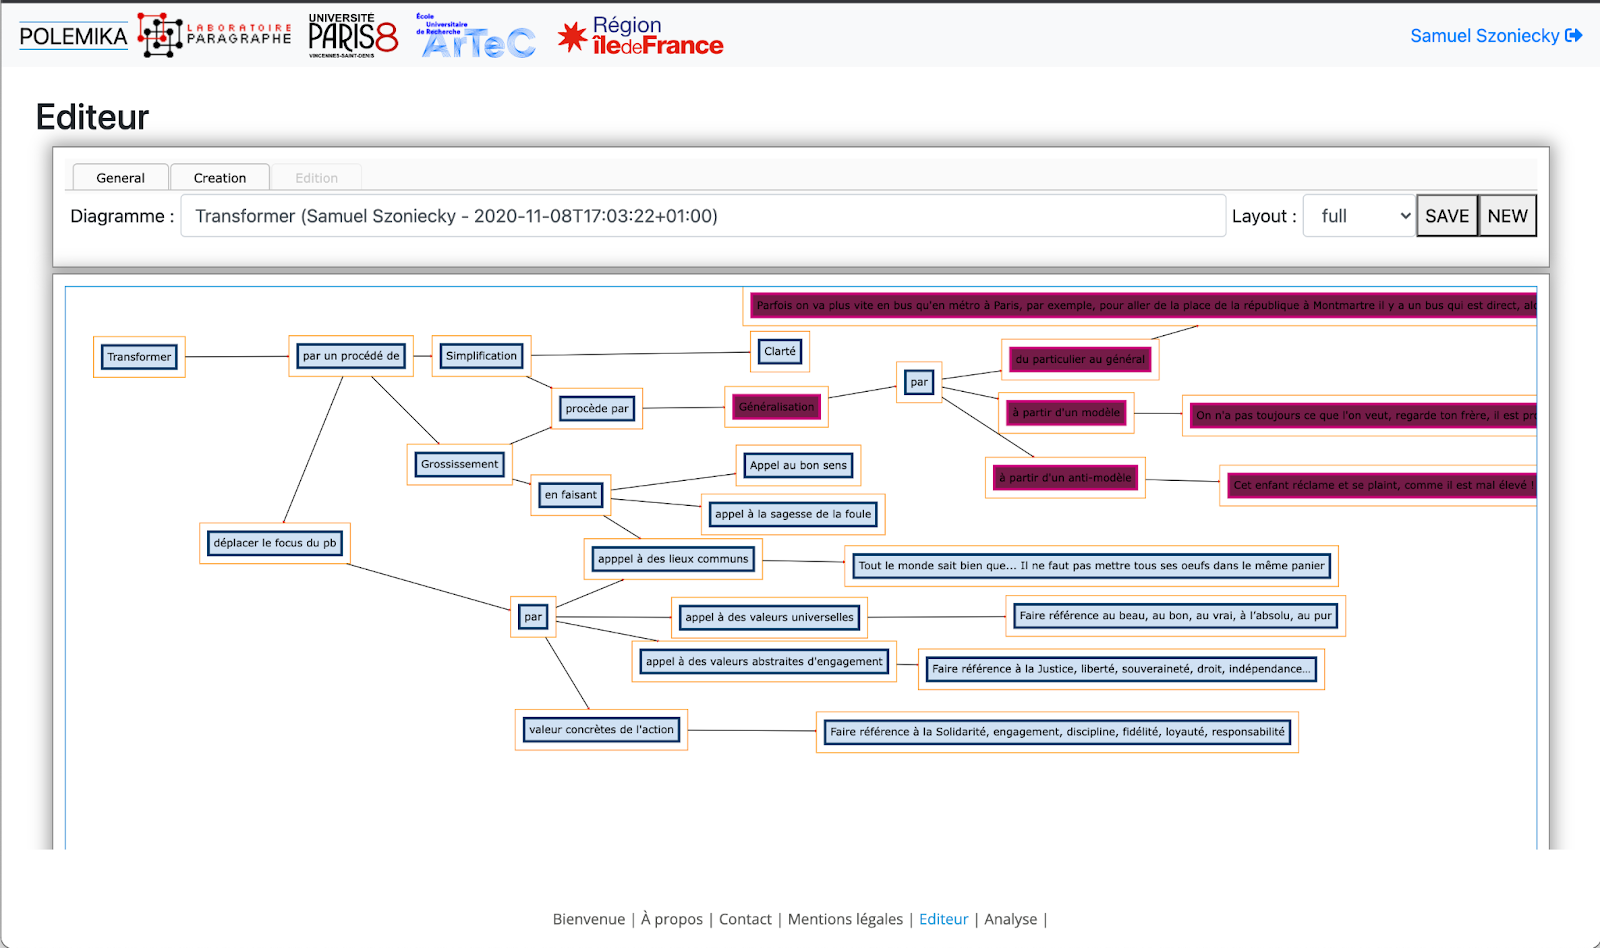
\includegraphics{images/polemikaEditor.png}

}

\caption{\label{fig-polemikaEditor}Editeur de cartographie conceptuelle}

\end{figure}%

\paragraph{Catégorisation des
informations}\label{catuxe9gorisation-des-informations}

Parallèlement au travaux menés lors du hackathon à la cité des sciences
et de l'industrie et lors des enquêtes en psychologie, nous avons
développé trois prototypes de catégorisation des fakes news afin
d'étudier en quoi un dispositif numérique permettrait de mieux
comprendre les processus cognitifs à l'oeuvre dans la réception des
informations. De plus, ces prototypes nous ont permis de valider ou pas
nos hypothèses ergonomiques.

\subparagraph{Catégorisation par roue}\label{catuxe9gorisation-par-roue}

Ce premier dispositif met en parallèle deux informations, une visuelle
et une textuelle. Les utilisateurs doivent catégoriser ces informations
à l'aide d'une roue qui déploie des concepts organisés hiérarchiquement
suivant une taxonomie conçue à partir de la catégorisation des mondes
sociaux(Desfriches Doria \& Meunier, 2021b).

Le dispositif a été développé sous la forme d'une application Web
autonome (https://github.com/samszo/polemika) puis intégré à Omaka S
sous la forme d'un thème spécifique :
https://github.com/samszo/polemika\_omks\_theme\_polemika

Le fonctionnement de ce processus de catégorisation est :

\begin{itemize}
\item
  visible dans cette vidéo :
  https://polemika.univ-paris8.fr/omk/s/contenus/page/processus-de-categorisation
\item
  utilisable dans cette page :
  https://polemika.univ-paris8.fr/omk/s/prototypes/page/qualification
\end{itemize}

\begin{figure}

\centering{

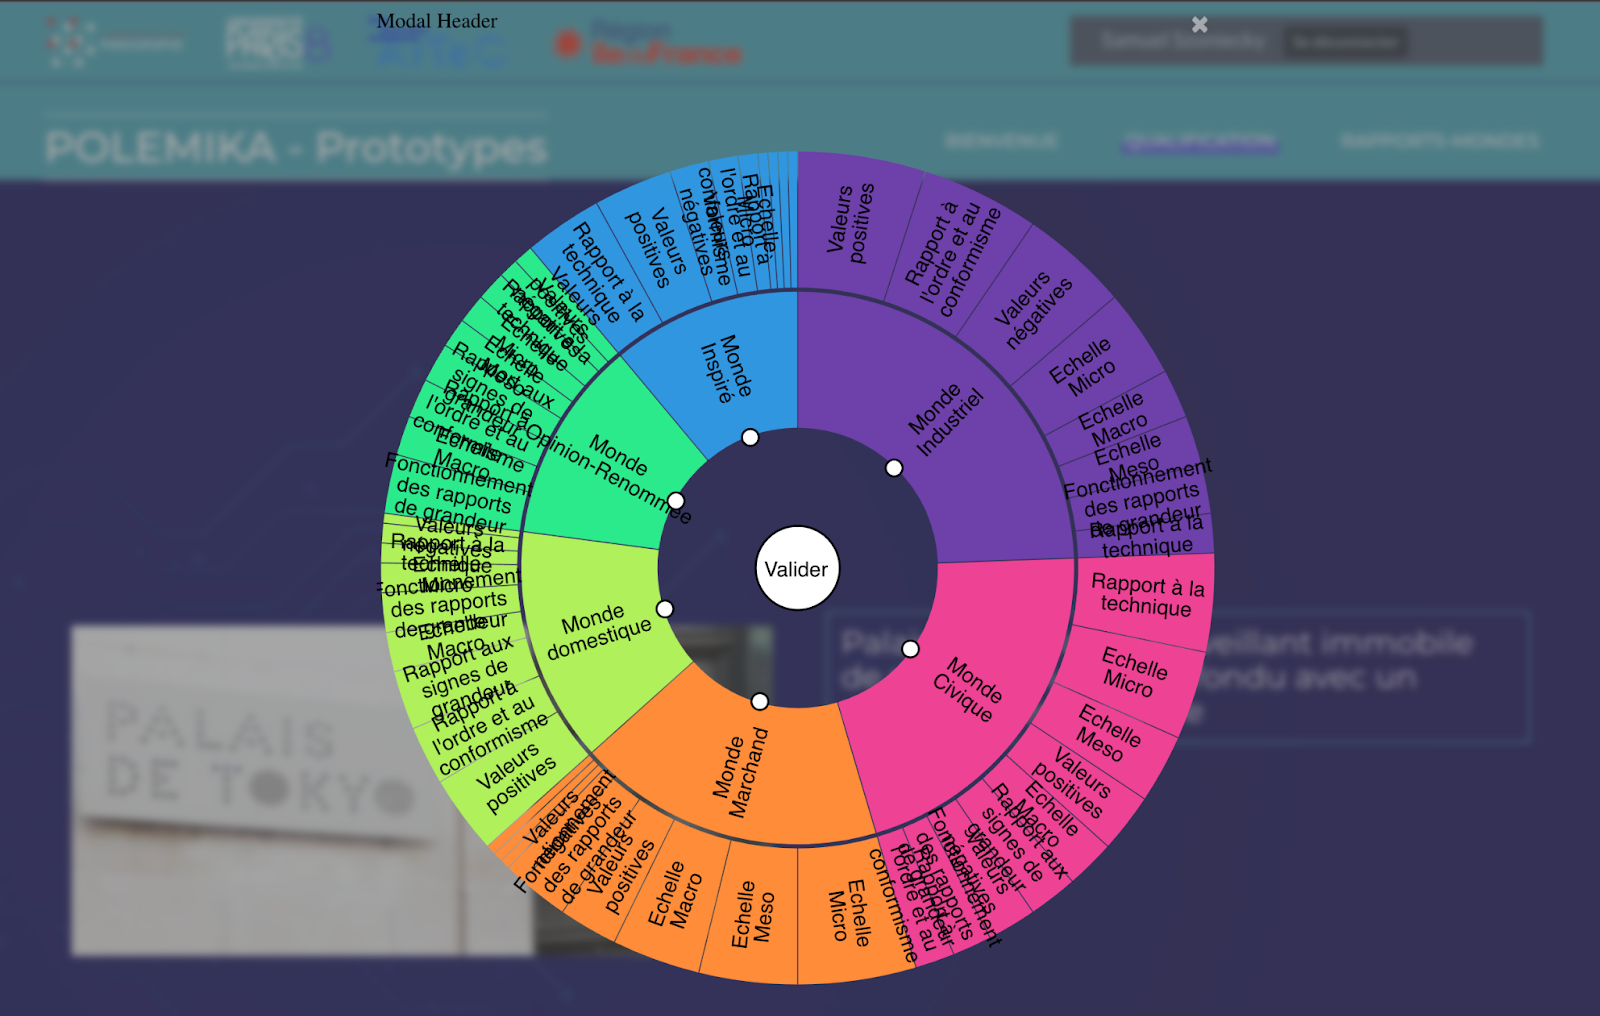
\includegraphics{images/polemikaRoue.png}

}

\caption{\label{fig-polemikaRoue}Catégorisation par roue conceptuelle}

\end{figure}%

L'interface développée n'est pas très ergonomique notamment au niveau de
la lisibilité des textes quand ils sont trop longs. De même, la
multiplication des clics rend le travail de catégorisation plutôt
laborieux.

\subparagraph{Catégorisation par validation des
cohérences}\label{catuxe9gorisation-par-validation-des-cohuxe9rences}

Ce second dispositif met lui aussi en relation deux informations mais
cette fois la représentation visuelles est mise en rapport avec un
réseau de concepts issu de la classification des mondes sociaux. Le
processus de catégorisation consiste à évaluer la cohérence entre la
photographie et le réseau de concept suivant une échelle allant de
``sans rapport'' à ``important''. Pour faciliter le travail de
catégorisation, une minuterie permet de changer automatiquement la photo
ou le réseau de concept. Le fonctionnement de ce processus de
catégorisation est : - visible dans cette vidéo :
https://polemika.univ-paris8.fr/omk/s/contenus/page/categorisation-par-validation-des-coherences
- utilisable dans cette page :
https://polemika.univ-paris8.fr/omk/s/prototypes/page/rapports-mondes

\begin{figure}

\centering{

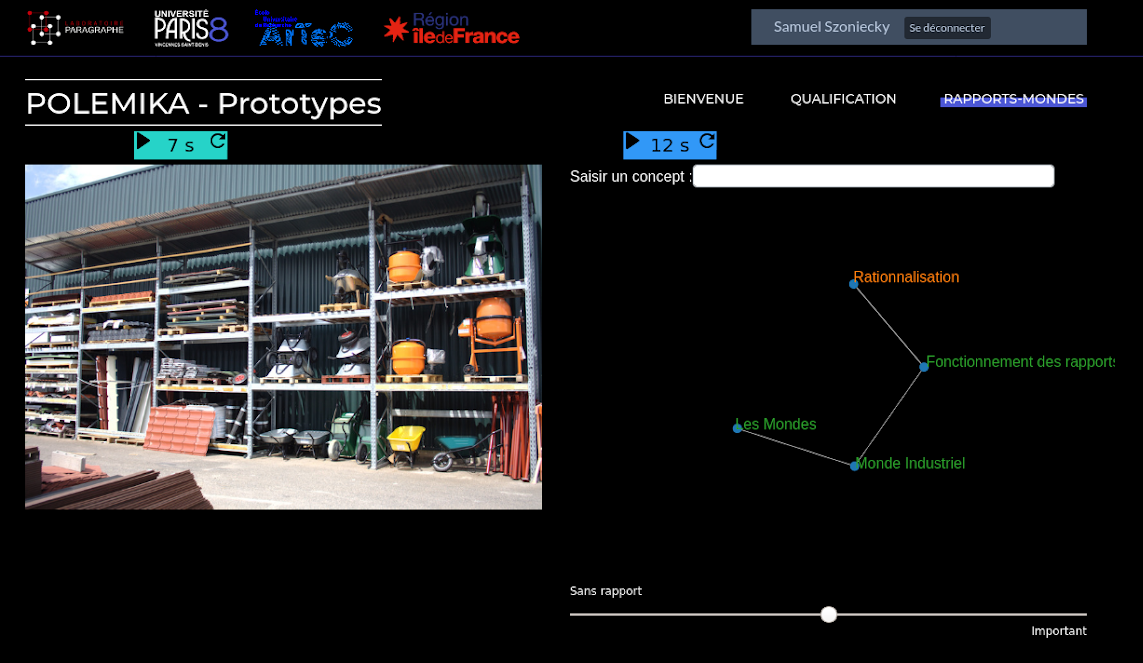
\includegraphics{images/polemikaReseau.png}

}

\caption{\label{fig-polemikaReseau}Catégorisation par validation des
cohérences}

\end{figure}%

\subparagraph{Catégorisation
émotionnelle}\label{catuxe9gorisation-uxe9motionnelle}

Ce processus de catégorisation utilise un jeu sérieux pour capter les
émotions produites par la consultation de fake news et visualiser
ensuite le résultat de cette évaluation pour la corriger et en faire une
analyse précise. Le fonctionnement de ce processus de catégorisation est
: - visible dans cette vidéo :
https://polemika.univ-paris8.fr/omk/s/contenus/page/categorisation-emotionnelle
- utilisable dans cette page :
https://polemika.univ-paris8.fr/omk/s/emotions/page/welcome

\begin{figure}

\begin{minipage}{0.50\linewidth}

\centering{

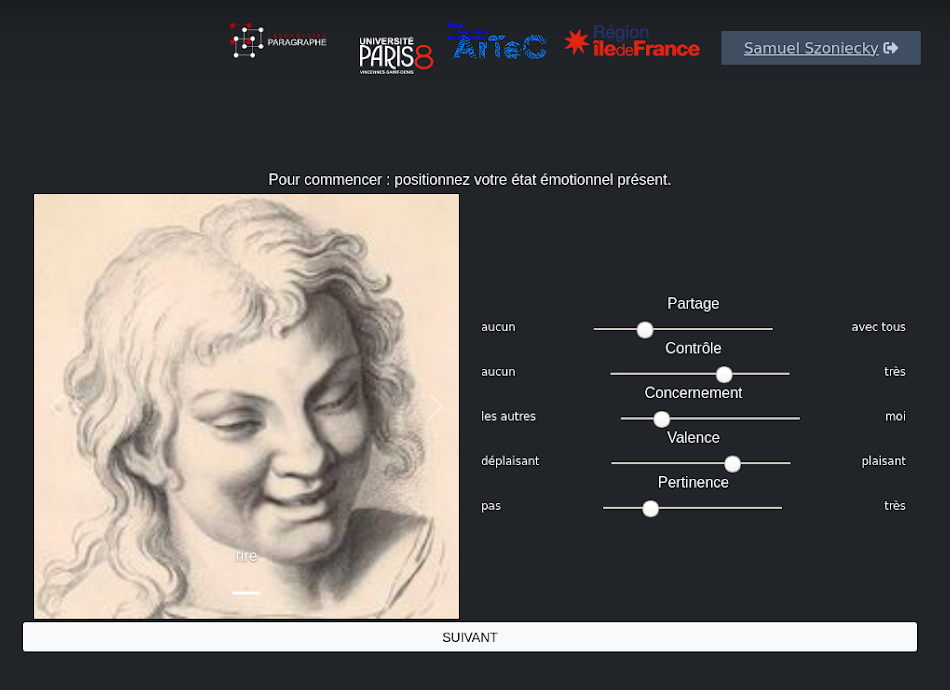
\includegraphics{images/polemikaEmotions.png}

}

\subcaption{\label{fig-polemikaEmotions1}Etape 1}

\end{minipage}%
%
\begin{minipage}{0.50\linewidth}

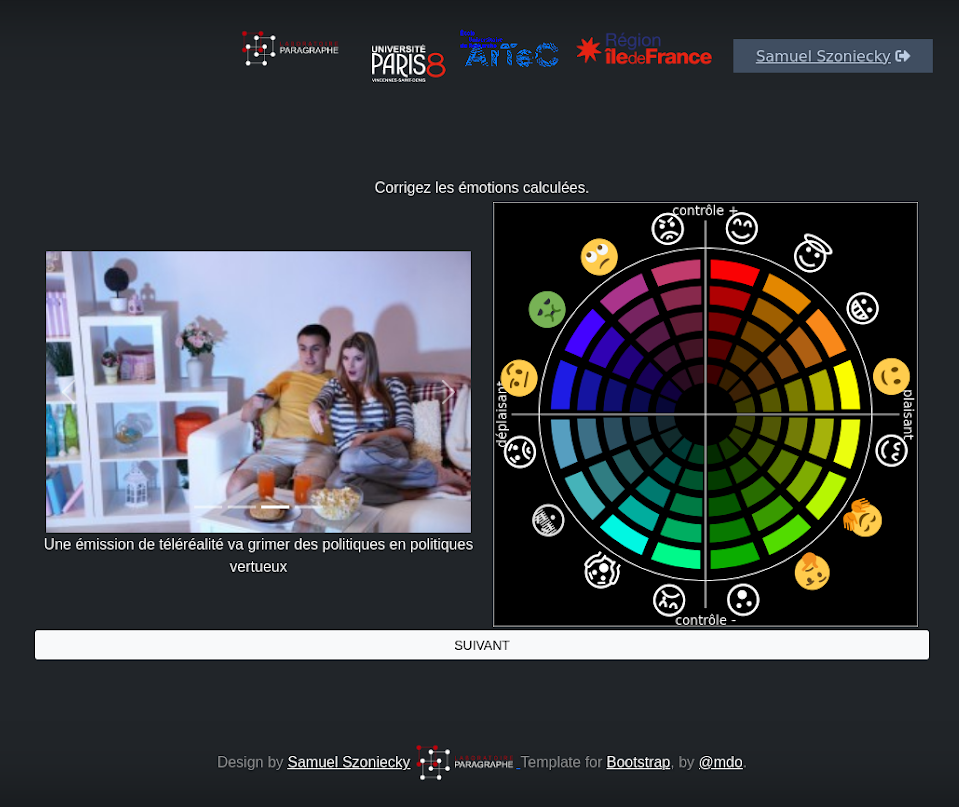
\includegraphics{images/polemikaEmotions1.png}

\subcaption{\label{}Etape 2}
\end{minipage}%

\caption{\label{fig-polemikaEmotions}Catégorisation émotionnelle}

\end{figure}%

\subsection[Projet Arcanes]{\texorpdfstring{Projet
Arcanes\footnote{Ce chapitre est issu de la demande de subvention CRSH}}{Projet Arcanes}}\label{projet-arcanespositionnements-7}

Le projet vise à étudier les régimes d'authenticité prenant place dans
une ère de post-vérité, soit les transformations des systèmes de vérité,
d'autorité et de légitimité à l'œuvre dans les dynamiques de médiations
contemporaines. Les objets de recherche visés, abordés de façon
intermédiale, sont situés à la fois dans la sphère des « arts
trompeurs~«, soit des arts recourant à la fois aux pratiques
illusionnistes et aux modes fictionnels en utilisant des stratégies de
tromperie, et dans celui des techniques de persuasion ou de manipulation
intervenant dans l'espace communicationnel actuel. Les deux modes
activent les « puissances du faux » .~Ils suscitent des imaginaires
sociaux qu'il s'agira d'étudier en les mettant en relation pour mieux en
exposer les rouages.~

Nos objectifs sont les suivants~:~

\begin{enumerate}
\def\labelenumi{\arabic{enumi}.}
\item
  Mener de façon interdisciplinaire une réflexion théorique en
  profondeur sur notre thème de recherche afin de développer une
  meilleure compréhension des mécanismes en jeu à la fois dans les arts
  trompeurs et dans l'espace informationnel qui seront significatives
  afin d'augmenter la littéracie numérique pour les clientèles visées
  (communauté universitaire et grand public).
\item
  Repérer, documenter et analyser les œuvres ainsi que les phénomènes de
  médiation contemporains relatifs à la question de l'authenticité,
  selon la perspective de l'intermédialité et de l'archéologie des
  médias, afin d'en retracer les filiations historiques et de mieux
  comprendre en retour leurs enjeux actuels.
\item
  Concevoir et développer un dispositif d'éditorialisation innovant dans
  le sillon des Humanités numériques, soit un écosystème de recherche à
  partir des avancées et des méthodes du Web sémantique afin de rendre
  compte de nos processus de recherche et résultats.~
\end{enumerate}

\subsubsection{Contexte}\label{contexte}

Ce projet se situe dans le contexte plus large des travaux du groupe de
recherche international Les arts trompeurs : Machines, magie, médias.
Active depuis 2015, cette communauté regroupe plus de 150 chercheurs
provenant d'une pluralité de disciplines et se consacrant aux pratiques
illusionnistes au cinéma, dans les arts vivants et les arts numériques,
ainsi qu'aux processus de fictionnalisation utilisés dans ces pratiques
et en littérature. Ce projet se situe également dans le prolongement
d'une subvention développement savoir du CRSH (Du spectacle magique au
numérique -SMEL, 2018-2020) qui centrait l'analyse sur les phénomènes de
médiation actifs dans le spectacle de magie, autour de la figure-phare
d'Houdini, à partir des archives inédites du Musée McCord. Il s'agissait
par la suite de comparer deux moments de médiation charnières (débuts
XXe et XXIe siècles) par des allers-retours permettant d'éclairer les
phénomènes contemporains de désinformation (Bourassa et als 2019b). Ces
premiers travaux ont confirmé toute la richesse et la profondeur de la
question de l'authenticité pour la recherche ainsi que ses impacts
majeurs dans les dynamiques de médiation contemporaines dans l'espace
public. Le présent projet marque une nouvelle étape décisive dans cette
réflexion afin d'approfondir notre compréhension du phénomène, par une
étude plus détaillée des « puissances du faux », en l'élargissant à
d'autres corpus et études de cas, tout en plaçant le phénomène en
relation avec ses filiations historiques pour mieux en comprendre, en
retour, les enjeux contemporains. Cette nouvelle étape sera aussi
marquée par une avancée importante sur le plan méthodologique, où nous
poursuivrons les développements amorcés dans SMEL pour l'exploitation
des données ouvertes (Linked Open Data) et des technologies du Web
sémantique.~

La diversité des champs que nous couvrons, des arts de la représentation
au Web sémantique, ainsi que nos origines disciplinaires variées
(design, cinéma, littérature, histoire de l'art, théâtre, génie
informatique et Humanités numériques) fondent le caractère
multidisciplinaire de ce projet.~ Cette approche interdisciplinaire
autour des questions relatives à l'authenticité en relation aux
dynamiques de médiation fonde également toute son originalité, car elle
permet de croiser des sphères de réflexion dans leur interdépendance, en
évitant d'isoler les phénomènes médiatiques à l'étude les uns des
autres, conformément à notre approche méthodologique basée sur
l'intermédialité.

\subsubsection{Axe d'éditorialisation numérique : développement d'un
écosystème de
connaissance}\label{axe-duxe9ditorialisation-numuxe9rique-duxe9veloppement-dun-uxe9cosystuxe8me-de-connaissance}

Dans ce projet j'ai particulièrement développé cet axe qui consiste à
adopter des méthodes d'Humanités numériques (HN) au moyen des techniques
du Web sémantique afin de rendre interopérables et calculables les
données récoltées et produites par la recherche. Un moissonnage
automatique de données (requêtes SPARQL) sera développé pour agréger et
structurer des contenus qui serviront de base au travail d'analyse des
chercheurs. En back end, l'écosystème sera soutenu par le CMS OmekaS
(données RDF natives et ontologies). Il inclura notamment des modèles de
carnets de recherche et de publication permettant la diffusion continue
de la recherche ainsi que l'activation de la communauté des Arts
trompeurs sous le mode de la conversation. Nous étendrons ce système par
des techniques d'intelligence artificielle pour la recherche
automatisée, afin d'investiguer plusieurs bases de données de façon
croisée, en transcendant les silos de données. Afin de générer et
d'analyser nos données, nous implanterons des méthodes de visualisation
pour en effectuer une modélisation~dynamique en mettant à profit les
principes cartographiques de la prétopologie (Levorato, 2008; Thibault,
2017) . Cette modélisation révélera des dynamiques de proximité et
d'éloignement qui nous permettront de représenter, de suivre et
d'analyser les multiples jeux de position (et les points de vue) qui
définissent les régimes d'authenticité et participent à leur
transformation.

Ces publications et ces projets donnent un bon aperçu de mon parcours
depuis ma thèse mais présentons maintenant de manière encore plus
précise mon écosystème de connaissances à partir des résultats de ma
veille informationnelle.

\section{Processus de veille pour créer un écosystème de
connaissances}\label{sec-processusVeille}

Depuis une quinzaine d'années, je mène un veille active pour à la fois
trouver, filtrer, organiser et diffuser les informations pertinentes
pour mes travaux de recherche et d'enseignement. Au fil du temps, j'ai
mis en place un processus spécifique pour effectuer cette tâche le plus
efficacement possible. Ce processus s'inspire des pratiques
professionnelles (Andro, Bondu, Dupin, \& Deschamps, 2022) que j'adapte
pour consacrer à ce travail une matinée par semaine.

\subsection{Sélectionner des sources}\label{sec-selectSources}

La première étape de ce processus de veille consiste à sélectionner des
sources d'informations qui me semble pertinentes pour explorer un
domaine de connaissances. Pour ce faire, j'utilise principalement deux
types de sources~: des e-mails et des flux RSS.

J'utilise les e-mails pour recevoir périodiquement des informations soit
en m'abonnant à des newsletters\footnote{\begin{quote}
  Liste des newsletters~: https://bit.ly/3KhDwY9
  \end{quote}} et des forums\footnote{\begin{quote}
  Liste des forums~: https://bit.ly/44KPfGX
  \end{quote}}, soit en utilisant le services d'alertes proposé par
Google, Google Scholar et HAL\footnote{\begin{quote}
  Liste des alertes~: https://bit.ly/3KgkSjz
  \end{quote}}. Pour les alertes, j'en ai paramétré une cinquantaine
portant soit sur des noms de chercheur soit sur des concepts. La veille
sur les noms de chercheur permet de connaître les nouvelles publications
de cette personne mais aussi comment il est cité par d'autres
chercheurs. Les alertes sur les concepts donne une bonne idée de
l'activité informationnelle dans un domaine. J'utilise aussi le service
de CAIRN pour recevoir automatiquement les nouvelles parutions des
revues scientifiques qui m'intéresse.

Pour consulter les flux RSS\footnote{\begin{quote}
  Liste des flux RSS~: https://bit.ly/3Yd9Z7V
  \end{quote}} que j'ai sélectionnés, j'utilise l'agrégateur de flux
Netvibes\footnote{\begin{quote}
  https://www.netvibes.com/
  \end{quote}} qui permet une lecture rapide des flux à partir du titre
des articles. Notons que la durée de vie d'un flux RSS est relativement
limité puisque sur le 180 flux que j'ai sélectionnés plus de la moitiés
ne sont plus opérationnels. Par exemple, le site d'Amazon ne met plus à
disposition de flux RSS pour suivre les parutions d'ouvrage dans un
domaine spécifique.

\subsection{Filtrer les informations}\label{sec-filtrerInfos}

La deuxième étape du processus de veille consiste à filtrer les
informations que les sources transmettent. Comme je reçois beaucoup
d'information des sources, le filtrage doit être rapide. Pour ce faire,
j'utilise un navigateur Web pour à la fois consulter les informations
fournies par les sources et accéder aux détails de celles-ci. Le premier
filtre se fait par une lecture des titres et parfois du résumé afin de
déterminer si l'information est pour moi pertinente ou pas. Si elle
l'est, j'active le lien hypertexte pour ouvrir dans un nouvel onglet les
détails. Quand j'ai fini la lecture de la source, je consulte les
onglets ouverts pour confirmer le filtrage et le cas échéant annoter
cette nouvelle référence.

\subsection{Annoter les références}\label{sec-annoterReference}

L'étape d'annotation des références est très importante car elle
consiste à enregistrer les informations pour enrichir ma base de
connaissances. Pour effectuer cette troisième étape du processus,
j'utilise deux outils complémentaires. Pour ce qui concerne les données
bibliographiques non numérisées, j'ai fait le choix de Zotero pour
enregistrer les références de la données et les annoter avec une liste
de mots clefs et des citations du document dans des notes. Notons que
Zotero ajoute automatiquement des mots clefs lorsque ceux-ci sont
précisés dans les métadonnées du document. Concernant les données du
Web, j'utilise l'outil d'annotation Diigo\footnote{\begin{quote}
  https://www.diigo.com/index
  \end{quote}} pour non seulement enregistrer l'URL d'un document Web
mais aussi le décrire avec des mots clefs, surligner avec différentes
couleurs une partie du document pour l'extraire et la commenter, faire
des copies d'écran pour conserver une partie de la page visualisée.

En terme d'indexation, cette étape d'annotation enregistre les rapports
entre des informations physiques concernant les références d'un document
et de ses parties, des informations conceptuelles à travers les mots
clefs utilisés, des informations sur l'actant qui fait l'annotation à un
moment donnée.

\subsection{Utiliser les annotations}\label{sec-utiliserAnnotations}

L'usage le plus fréquent que je fais des annotations consiste à
référencer nos écrits scientifiques en utilisant des URLs ou des données
bibliographiques que j'intégre directement dans le texte grâce au
connecteur Zotero\footnote{\begin{quote}
  https://tutos.bu.univ-rennes2.fr/c.php?g=686436\&p=4906338
  \end{quote}}, comme c'est le cas dans ce travail. Les références
enregistrées dans ma base de connaissances se retrouvent facilement en
faisant une recherche par mot clef ou en plein texte. Les résultats de
ces recherches donnent une liste de documents dont les annotations font
office de résumé. En visualisant les mots clefs utilisés et les parties
sélectionnées, il n'est plus nécessaire de consulter l'intégralité du
document. Par exemple, voici la page d'annotation d'un article dans
Diigo~:

\begin{figure}

\centering{

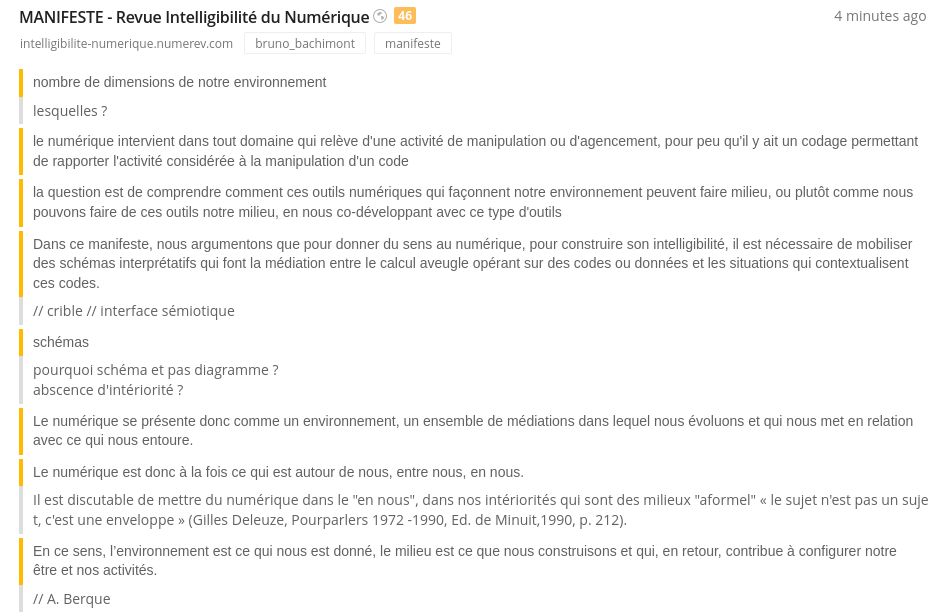
\includegraphics{media/10000001000003A4000002648983E64502CE7461.png}

}

\caption{\label{fig-annotationDiigo}Article annoté dans Diigo}

\end{figure}%

Cette copie d'écran montre les parties de l'article que j'ai
sélectionnées (marge jaune) et les notes que j'ai prises pour la
sélection (marge grise). En ce référent à cette page d'annotation, il
est pratique de retrouver rapidement ce qui m'a semblé pertinent et
pourquoi\footnote{\begin{quote}
  Dépôt du projet~:
  \url{https://gitlab.com/Daniel-KM/Omeka-S-module-BulkImport}
  \end{quote}}.

Un autre usage particulièrement intéressant des annotations est la
conservation des références qui ne sont plus accessibles en ligne et qui
représente dans notre corpus plus de 10~\% des URL (cf.~ci-dessous).
Lorsque nous importons les annotations Web depuis Diigo vers ma de base
de connaissances Omeka S Section~\ref{sec-importDiigo}, je teste la
validité de l'URL et enregistre son statut\footnote{\begin{quote}
  Tableur d'importation des données du CV dans Omeka s~:
  \url{https://docs.google.com/spreadsheets/d/1ap0Q6l8bK9Y8wB21xfCAk9qeJ-Gfa6XAjO-cVk2LxdI/edit?usp=sharing}
  \end{quote}} ce qui permet de savoir quelles URL sont obsolètes~:

\begin{figure}

\centering{

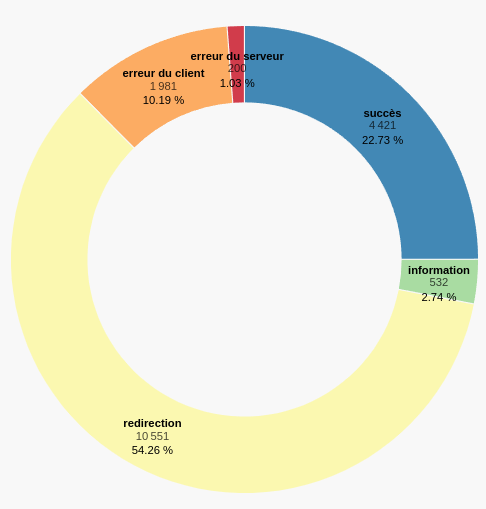
\includegraphics{media/10000001000001E6000001FDFBA335D820BED6E2.png}

}

\caption{\label{fig-statutUrlDiigo}Répartition de la classe des statuts
pour les URL dans Diigo}

\end{figure}%

L'usage le plus intéressant de cette base de données d'annotations est
sans doute leurs analyses pour une gestion des connaissances
personnelles (Deuff, 2012) et la cartographie d'un milieu de
connaissance qui est l'objet de ce travail.

De manière plus expérimentale, nous utilisons ces annotations pour
développer de nouvelles formes d'éditorialisation scientifiques en
puisant dans cette base de données la matière d'une inspiration
chaotique Section~\ref{sec-chaoticumSeminario}.

\subsection{Diffuser les annotations}\label{sec-diffuserAnnotations}

Ce travail d'annotation et de sélection de citation me fourni une base
de connaissances de plus de 1 400 références bibliographiques et plus de
19 000 références Web qui sont indexées par plus de 6 000 concepts.
L'ensemble de ces données sont accessibles soit sur les Zotero pour les
références bibliographiques\footnote{\begin{quote}
  Tableur d'importation des données GitHub dans Omeka s~:
  \url{https://docs.google.com/spreadsheets/d/1W92NdhcMurFO96Et82MOYL43fvFrdOB6nLGF-QeCrkY/edit?usp=sharing}
  \end{quote}}, soit sur Diigo pour les références Web\footnote{\begin{quote}
  https://www.diigo.com/user/luckysemiosis
  \end{quote}}, soit directement dans mon site Omeka S dans un format
HTML pour naviguer dans la base de données ou en JSON\footnote{\begin{quote}
  https://samszo.univ-paris8.fr/omk/api/items?item\_set\_id=1\&item\_set\_id=4
  \end{quote}} pour analyser les données avec des algorithmes.

\subsection{Réfléchir le processus}\label{sec-reflechirProcessus}

Le processus que nous venons de décrire évolue constamment, tend à
s'améliorer, se préciser au fil du temps et s'enrichir de nouvelles
pratiques. Par exemple, une analyse automatique de l'adéquation entre
les sources d'information, les données filtrées, les annotations et
leurs utilisations dans des travaux scientifiques ou pédagogiques,
pourrait servir de base pour un système de recommandation (Hachour,
Szoniecky, \& Abouad, 2014).

Toutefois, le fait que les étapes du processus soient principalement
manuelles contribue à construire une subjectivité qui m'est propre.
Chaque décision nécessaire pour la poursuite du processus est prise
parce qu'au moment du choix elle correspond aux inclinaisons de ma
«~raison trajective~» Figure~\ref{fig-cyclesemiose} . En enregistrant
ces décisions via des dispositifs numériques, le processus de veille
offre dès lors un triple intérêt. Premièrement, il permet d'explorer
rationnellement une domaine de connaissances. Deuxièmement, elle trace
un frayage (Citton, 2010) particulier dans un écosystème de
connaissances qui crée les conditions d'une communication stigmergique~:

\begin{quote}
«~L'étymologie grecque explique assez bien le sens du mot « stigmergie »
: des marques (stigma) sont laissées dans l'environnement par l'action
ou le travail (ergon) de membres d'une collectivité, et ces marques
guident en retour -- et récursivement -- leurs actions.~»~(Lévy, 2023b)
\end{quote}

Troisièmement, il donne une représentation d'une subjectivité et de ces
évolutions ce qui conditionne le développement de la réflexivité et de
l'esprit critique (Desfriches Doria \& Meunier, 2021a).

Entre l'automatisation du processus et les choix manuels, il convient
donc de pratiquer le bon équilibre entre alléger le travail et
construire son esprit critique \textbf{?@sec-part-technoIntello}.

\section{Cartographie existentielle de mon écosystème de
connaissances}\label{cartographie-existentielle-de-mon-uxe9cosystuxe8me-de-connaissances}

A partir du processus de veille que nous venons de décrire, j'ai
constitué une base de connaissances qui reflète de manière très précise
mon environnement scientifique et intellectuel. Pour faciliter le
traitement des données de cette environnement nous les avons
centralisées dans Omeka S qui représente une base de données SQL de 75
tables peuplées par plus de 2 000 000 de lignes\footnote{L'ensemble de
  ces données sont accessibles via l'API de Omeka S sous un format
  RDF-JSON utilisé pour l'interopérabilité entre les machines mais aussi
  via des représentations dédiées à la navigation à l'intérieur de cet
  écosystème.}. Le graphique ci-dessous présente la répartition des
objets disponibles dans cet écosystème suivant leur classe\footnote{\begin{quote}
  Les données de ce graphique et d'autres statistiques sont disponibles
  ici~: \textless omkStats.html\textgreater{}
  \end{quote}}~:

\begin{figure}

\centering{

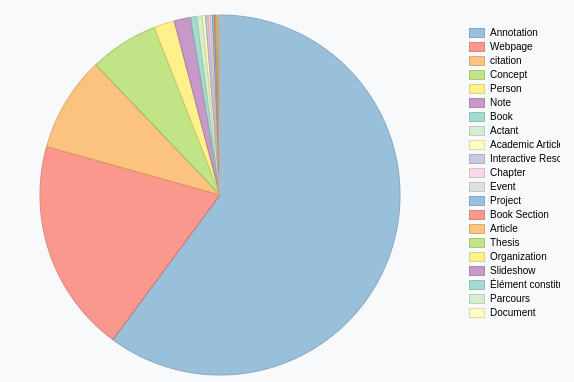
\includegraphics[width=11.09cm,height=7.378cm]{media/100000010000023E0000017E87A6A293BEC71C5E.png}

}

\caption{\label{fig-repartitionClass}Répartition des classes par nombre
d'objet dans l'écosystème}

\end{figure}%

Le graphique montre que les deux tiers des objets dans l'écosystème sont
des annotations (61 120 = 60~\%) qui créent un rapport entre un
document, un actant et un concept. Nous retrouvons ici le 4 dimensions
du modèle que nous utilisons pour modéliser les connaissances
(Section~\ref{sec-modeleOntoEthique}) : document, actant, concept,
rapport. Plus précisément, la dimension physique (documentaire) est
composée essentiellement de pages Web (19 491 items = 19~\%\footnote{\begin{quote}
  Liste complète des pages Web~: \url{https://bit.ly/3Qj1NRm}
  \end{quote}}), des citations (8 994 = 9~\%), de médias (3 427 = 3~\%),
des notes (1 488 = 1~\%) et des livres (568 = 1~\%) issues de notre
processus de veille. Les autres dimensions de l'écosystème sont les
concepts (6 266 = 6~\%) et les personnes (1 898 = 2~\%) associées aux
actants (500 = 0,5~\%). Le graphique ci-dessous montre cette répartition
des objets suivant les dimension existentielles~:

\begin{figure}

\centering{

\includegraphics[width=11.185cm,height=8.019cm]{media/100000010000021900000181A00CD43E3311E6DF.png}

}

\caption{\label{fig-repartitionDimExi}Répartition des objets par
dimension existentielle}

\end{figure}%

Cette représentation suivant la classe des objets sous estime la
complexité de l'écosystème puisqu'elle ne prend pas en compte le détails
des valeurs (dimension physique) de chaque propriété (dimension concept)
ni l'actant qui exprime les rapports entre propriétés et valeurs, encore
moins l'évolution de cette complexité au fur et à mesure que
l'écosystème se transforme. Pour une meilleur compréhension de
l'écosystème, nous considérons chaque donnée comme une existence
particulière qui possède ça propre complexité qui s'ajoute à la
complexité de l'ensemble. Cette complexité de l'objet est d'autant plus
grande que la valeur d'une propriété est une ressource sous la forme
d'une URI vers une page Web ou un lien vers une autre existence de
l'écosystème est donc vers une nouvelle complexité qui elle aussi
s'ajoute à la complexité globale. A partir des règles génériques pour
calculer la complexité existentielle d'un écosystème
(Section~\ref{sec-complexiteExitentielle}), nous obtenons pour
l'écosystème de connaissances de ce travail une complexité de 38.4589
Millions, ce qui est très important en comparaison de la complexité
d'une citation d'ouvrage qui varie entre 60 et 3 000 mais ce qui est
très peu par rapport à la complexité d'une bibliothèque, de wikipédia ou
d'une IA générative comme ChatGPT
(Section~\ref{sec-modeliserEcosystemeReference}). Ce chiffre prend en
compte l'ensemble des existences informationnelles qui peuplent notre
base de connaissance, il nous est utile pour comparer les connaissances
potentielles de ces existences dont on peut représenter la répartition
suivant leur niveau de complexité (abscisse) et le nombre d'existence
pour chaque complexité (ordonné) :

\begin{figure}

\centering{

\includegraphics{images/localhost_samszo_HDR_jdcComplexity.html.png}

}

\caption{\label{fig-RepartitionComplexity}Répartition de la complexité
des existences dans l'écosystème \href{jdcComplexity.html}{voir en
ligne}}

\end{figure}%

Ce graphique montre que la complexité des existences est très diverse
puisqu'elle s'établit entre 1 et presque 3 Millions, de même concernant
le nombre d'existence ayant la même complexité qui oscille entre 1 et
plus de 10 mille. Une analyse des répartitions suivant le type de
ressource omeka (media, item, collection, annotation) montre que les
ressources les moins complexes sont les médias avec une complexité
inférieure à 12 et les plus complexes sont bien évidemment les
collections car elles cumulent les complexités des ressources qui la
compose.

Il reste encore de nombreuses travaux de recherche à faire sur cet
écosystème de connaissances, ces évolutions, les moyens de les modéliser
et de les analyser. Nous détaillerons plus loin les principes de
cartographie des connaissances que nous avons élaboré à partir de cette
écosystème Chapter~\ref{sec-principesCarto} et le programme de recherche
que nous souhaitons développer Chapter~\ref{sec-visees} . Mais pour le
moment focalisons-nous sur un aspect particulier en analysant les
personnes présente dans l'écosystème.

\section{Les personnes de mon écosystème de
connaissances}\label{sec-personneEcoCon}

L'écosystème de connaissances que j'ai constitué à partir de mon travail
de chercheur et d'enseignant compte plus de 2 000 personnes. Parmi cette
foule, j'entretiens des rapports très différents avec chacune des
personnes, certaines sont des amies, d'autres des collègues ou des
auteurs que j'ai lu sans jamais les rencontrés\ldots{} De plus, ces
rapports évoluent dans le temps au fil des rencontre intellectuelles et
amicales. Pour décrire ces relations, nous pourrions nous inspirer des
propositions de Gabrielle Tarde (Citton, 2008b) pour réaliser une
économie des affects à partir de trois registres : les «
valeurs-utilités », les « valeurs-vérités » et les « valeurs-beautés.
Nous verrons en détails Section~\ref{sec-confianceDonnees} comment à
partir de ces propositions concevoir une cartographie des affects mais
il est difficile d'appliquer cette méthode ici, sans potentiellement
créer des difficultés dans les relations que j'entretiens avec ces
personnes. En effet, que dire à un ou une collègue qui me demande
pourquoi les ``valeurs'' que je lui attribue sont moindres que celle
d'un ou d'une autre ? Pour éviter ce type de situation, je n'applique
pas cette méthode ici car elle exacerbe trop ma subjective mais je
privilégie une approche plus objective en analysant la place de ces
personnes dans mon écosystème de connaissances.

Premièrement, nous allons examiner l'importance de ces personnes dans
mon écosystème de connaissances à partir d'un WordsStream\footnote{Nous
  avons adapté ce diagramme proposé originalement par
  \href{https://github.com/huyen-nguyen}{Huyen Nguyen}
  \url{https://github.com/iDataVisualizationLab/WordStream} pour mieux
  piloter les données et leurs visualisations. Le code du module que
  nous avons développé est ici :
  \url{https://github.com/samszo/HDR/blob/main/docs/modules/streamWords.js}}
. Ce diagramme montre comment l'importance des items d'une catégorie
évolue dans le temps. Dans notre écosystème, cette importance est
calculée par le nombre de fois qu'une personne est en rapport avec une
existence de l'écosystème\footnote{Les données de calcul sont
  accessibles ici :
  \url{http://localhost/samszo/omk/s/cartoaffect/page/ajax?json=1&helper=JDC&action=getStream&id=61225}}.
Nous avons catégorisé ces existences suivant les quatre dimensions de
notre modèle\footnote{l'algorithme de classification est disponible ici
  :
  \url{https://github.com/samszo/Omeka-S-module-JDC/blob/master/src/View/Helper/JDCViewHelper.php\#L234}}
(actants = 2 000, concepts = 822, document = 1214, rapports = 11 777)
puis nous avons regroupé les rapports en 4 groupes :

\begin{itemize}
\item
  les personnes qui sont co-auteur de mes publications (bleu)
\item
  les personnes qui ont participées à mes projets (vert)
\item
  les auteurs de mes références bibliographiques (rouge)
\item
  les auteurs des références pour lesquelles j'ai fait des annotations
  (orange).
\end{itemize}

Le diagramme obtenu représente l'évolution dans le temps de l'importance
des personnes dans ces 4 catégories :

\begin{figure}

\centering{

\includegraphics{images/localhost_samszo_HDR_docs_jdcStreamTot.png}

}

\caption{\label{fig-wordstreamTot}Evolution de l'importance des
personnes de l'écosystème}

\end{figure}%

L'image ci-dessus montre la totalité du diagramme pour les quatre
catégories. Cette représentation ne permet pas de voir les détails que
nous traiterons plus loin mais révèle tout de même quelques points
important :

\begin{itemize}
\item
  les références bibliographiques de mon écosystème de connaissances
  couvre une grand période temporelle (1515 - 2024) mais principalement
  le XXIème siècle. Toutefois, il faudrait corriger les données en
  prenant en compte non pas la date de publication de la référence
  bibliographique mais la date de création par l'auteur. Par exemple, la
  référence bibliographique (Peirce \& Tiercelin, 2003) possède une date
  de publication en 2003 mais les écrits de Peirce regroupés dans ce
  volume ont été produits après 1880 et avant 1914. Nous n'avons pas
  pour l'instant ces données pour l'ensemble de nos références
  bibliographiques mais nous pourrions les calculer à partir des dates
  de naissance et de mort des auteur. Ce travail reste à faire.
\item
  On note une baisse de l'importance du flux en 2012 et en 2020. La
  première date correspond à une activité importante de recherche de
  2009 à 2012 lié à la thèse puis à sa rédaction et la seconde à la
  crise du COVID.
\item
  La part des publications (bleu) est très petite par rapport aux
  autres. Ceci correspond tout à fait au principes de référencement des
  sources dans une publication universitaire puisque pour un article
  publié, il y a en moyenne une dizaine de références.
\end{itemize}

\begin{figure}

\centering{

\href{http://localhost/samszo/HDR/docs/jdcStream.html?cat=publications}{\includegraphics{images/localhost_samszo_HDR_docs_jdcStreamPublications.png}}

}

\caption{\label{fig-wordstreamPublications}Evolution des co-auteurs de
mes publications}

\end{figure}%

En regardant plus en détail les co-auteurs de mes publications
Figure~\ref{fig-wordstreamPublications} , on distingue que la majeure
partie des co-auteurs sont des collègues du laboratoire Paragraphe même
si depuis 2022 je collabore davantage avec des collègues venant d'autres
institutions notamment en lien avec les projets de l'EUR
ArTec\footnote{lien vers le site : \url{https://eur-artec.fr/}} et de
l'Université Européenne EURUA\footnote{lien vers le site :
  \url{https://erua-eui.eu/}}

\begin{figure}

\centering{

\href{http://localhost/samszo/HDR/docs/jdcStream.html?cat=projets}{\includegraphics{images/localhost_samszo_HDR_docs_jdcStreamProjet.png}}

}

\caption{\label{fig-wordstreamProjet}Evolution des personnes
participants aux projets}

\end{figure}%

Le diagramme des personnes participants aux projets
Figure~\ref{fig-wordstreamProjet} montre clairement l'augmentation des
collaborations à partir de 2013 date à laquelle mon utilisation de
GitHub devient plus importantes et par la même accroît les possibilités
de travail collaboratif notamment avec les étudiants.

\begin{figure}

\centering{

\href{http://localhost/samszo/HDR/docs/jdcStream.html?cat=annotations}{\includegraphics{images/localhost_samszo_HDR_docs_jdcStream.html_cat=annotations.png}}

}

\caption{\label{fig-wordstreamAnnotations}Evolution des personnes dont
les publications sont annotées}

\end{figure}%

Le diagramme ci-dessus Figure~\ref{fig-wordstreamAnnotations} montre
l'évolution de l'importance des personnes dont j'ai annoté les
publications suivant le principe que plus j'ai annoté leurs publications
plus elles sont importantes. Les annotations commencent en 2009 ce qui
correspond au début de mon usage de Zotero
Section~\ref{sec-annoterReference}. Pour donner une représentation plus
complète de mon travail d'annotation des références bibliographiques, il
faudrait numériser les notes que je prises sur du papier et plus encore
expliciter les notes prises directement dans les ouvrages
Figure~\ref{fig-annotationsLivre}. Ce travail pourrait être fait avec
les outils d'annotations d'image d'Omeka S mais cela dépasse le cadre de
cette HDR.

\begin{figure}

\centering{

\includegraphics{images/annotationsLivre.jpeg}

}

\caption{\label{fig-annotationsLivre}Annotations d'un livre}

\end{figure}%

Même si ce diagramme n'est pas exhaustif, il montre les personnes les
plus importantes de mon parcours intellectuel. Ces personnes ne sont pas
toutes spécialistes des sciences de l'informations et de la
communication mais m'ont apportés des notions éclairantes pour mon
travail de recherche. Je pense notamment à Gilles Deleuze que je lis
depuis une trentaine d'années et que j'écoute régulièrement

\chapter{Perspectives scientifiques~: échelles d'exploration et axes
d'expérimentation}\label{sec-visees}

Au delà de nos positionnement actuels que nous venons de présenter
Section~\ref{sec-posiSIC} notre travail de recherche se déploie suivant
plusieurs perspectives que nous développeront ici suivant les
diffférents niveaux d'échelles que nous explorons et les axes
d'expérimentations que nous développons afin de mettre fin à un «
amincissement du monde » et une représentation de la pensée en un réseau
qui supprime la multiplicité des modes d'existences~:

\textgreater{} «~Tout se passe comme si la densité des modes
d'existence, la pluralité des relations que nous pouvons entretenir avec
les êtres qui forment nos milieux et qu'ils entretiennent entre eux,
l'hétérogénéité de nos savoirs, cette « surabondance du réel » étaient
la cible d'un leitmotiv : une seule logique pour l'hétérogénéité des
savoirs, un seul mode d'existence pour la pluralité des êtres, un seul
cosmos pour la diversité des mondes. Bref, cette peur d'être dupe a pour
effet de réduire les savoirs, les êtres et le monde à une seule et
unique couche d'existence.~» (Debaise \& Stengers, 2021, sec. 6)

Ce qui nous importe ici c'est de lutter contre une « politique de la
méfiance »(Guattari, 1989), réduisant les environnements à une simple
ressource en usant de catégories qui rendent équivalentes ou
insignifiantes les manières d'habiter, de s'attacher, de valoriser. Ce «
laminage des subjectivités\,» (\emph{Ibid.}) entraîne la destruction des
rapports collectifs par une mise en concurrence généralisée à tous les
niveaux des individus entre eux. Voyez donc ici l'expression d'une
subjectivité qui donnera lieu j'espère à une politique de la curiosité
conduisant au développement d'un collectif de pensé stimulé par la
différence.

\section{Echelles d'exploration}\label{sec-echelleExploration}

\subsection{Echelle locale : produire une expression
matérielle~cohérente}\label{sec-echelleLocale}

Concevoir des outils sur des mobiles

\section{Echelle globale : technologies intellectuelles
collectives}\label{sec-echelleGlobale}

Rendre interopérables les données produites

\section{Echelle sociale~: la communauté des enseignants
chercheurs}\label{sec-echelleSociale}

Pas uniquement à l'université~: tout acteur est à la fois chercheur et
enseignant = explorateur et conteur.

Détailler l'importance de ce point de vue dans le cadre de
l'enseignement où la notion de gestion de l'information n'est pas
évidente\ldots{}

\section{Echelle conceptuelle~: théoriser la modélisation des
connaissances}\label{sec-echelleConcetuelle}

Fournir une alternative qualitative à la théorie de l'information de
shannon

\section{Axe internet des objets}\label{sec-axeIOT}

Concevoir, développer et analyser les objets connectés dans un Internet
omniprésent

\section{Axe écritures génératives}\label{sec-axeGeneratif}

Les exemples de data visualisation ci dessus illustrent ce qui est en
jeu

Représentation paramétrique de données

Traduction, transformation numérique~?

Intelligibilité du modèle~?

Choix entre spécificité, généricité et réutilisabilité~?

cf.~\url{https://levelup.gitconnected.com/how-to-make-your-code-reusable-891ea5db415c}

\section{Axe plasticité absolue}\label{sec-axePlasticite}

``Contrairement à l'élasticité, la plasticité n'a aucune promesse de
retour. Les deux concepts suggèrent un point limite auquel le système se
rompt. Cependant, le changement dans chacun est différent, car quelque
chose d'élastique revient ou peut reprendre forme après son changement.

Contrairement aux compréhensions du pouvoir, même aux formes subtiles de
pouvoir disciplinaire, la plasticité à l'échelle de l'individu et de la
polis représente la possibilité d'un changement sans sujétion,
c'est-à-dire sans résistance. Plutôt que les relations de pouvoir qui
font des sujets à l'image foucaldienne, on a la possibilité de concevoir
ou de diriger des sujets qui n'ont aucun indice de ce qu'ils étaient
avant, de sorte que quelque chose puisse résister.'' mail Jean Max

https://mail.google.com/mail/u/0/?tab=rm\&ogbl\#inbox/FMfcgzGtwMVVsTKtkHmLcCDbcHMMTbbd

\section{Axe design des connaissances}\label{sec-axeDesignConnaissances}

Modélisation des connaissances et conception des outils pour la
manipuler dans les environnements d'apprentissage humain

Mise en situation d'une potentialité de connaissances

Comment concevoir une ergonomie des interfaces cognitives~?

Passage de l'individuel au collectif~?

- premier langage~: enseignement de math et des stats

Modèle sémiologique + anthropologique + onto éthique

\section{Axe intelligences collectives}\label{sec-axeIntelCo}

Interopérabilité et réflexivité d'une conversation créative

=\textgreater{} fournir les outils pour une quantification de
l'information et la stimulation des communications

\section{Axes formalisation du consensus}\label{sec-axeFormaConsensus}

Méthodes et outils du web sémantique et du LOD~: la puissance de la
norme.

Pour une éthique de la discussion par une formalisation des échanges
ayant pour but l'éducation de l'esprit critique par la stimulation des
trois pouvoirs de discerner, choisir, agir.

Les deux textes ci-dessus ont été générés par deux IA à partir du titre
de la séance du séminaire. Leur pertinence toute relative illustre les
effets du pilotage par les données du métier de chercheur en SHS d'un
point de vue éthique : stimuler ``une formation de la volonté'' à
travers des règles pratiques d'échanges (Habermas 2013, p.~22).

L'enjeu de l'éthique est d'exercer sa ``volonté'' en tant qu'individu ou
qu'institution face à une situation de choix : ``L'éthique classique,
comme d'ailleurs les théories modernes, partent de la question qui
s'impose à un individu ayant besoin d'orientation lorsque dans une
certaine situation, il se trouve, indécis, devant une tâche à maîtriser
pratiquement : comment dois-je me comporter, que dois-je faire ?''
(ibid. p.~96). Contrairement à une volonté politique, la ``volonté
éthique'' ne s'exerce pas sur les ``physicalités'' (Descola 2005)
extérieures en cherchant par exemple à éliminer les biais inhérents à
toutes informations nécessairement inadéquates, mais se pratique dans la
dimension des idées, celle de ``l'intériorité'' (ibid.) individuelle ou
collective :

``Tout dans l'existence nous condamnait à n'avoir que des idées
inadéquates : nous n'avions ni l'idée de nous même, ni l'idée des corps
extérieurs, mais seulement des idées d'affections, indiquant l'effet
d'un corps extérieur sur nous. Mais précisément, à partir de cet effet,
nous pouvons former l'idée de ce qui est commun à un corps extérieur et
au nôtre. Compte tenu des conditions de notre existence, c'est pour nous
la seule voie capable de nous mener à une idée adéquate. La première
idée adéquate que nous ayons, c'est la notion commune, l'idée de
ce''quelque chose de commun''.'' (Deleuze 1968 p.~259)

Pour parvenir à ce ``commun'', nous avons élaboré une multitude de
``jeux de langages'' (Wittgenstein 1987), de diagrammes (Guattari 1989),
de dispositifs (Gardies 2012)\ldots{} dont ceux utilisés aujourd'hui par
les chercheurs pour produire grâce au numérique une infinité de
``physicalités'', de documents, de données, de ressources. Ce
développement exponentiel des physicalités renvoie les chercheurs à deux
questions éthiques fondamentales :

Comment exercer nos volontés éthiques dans cette noosphère pilotée
exclusivement par des machines ? Peut-on concevoir des documents pilotés
par des données (https://d3js.org/) dédiés à l'exercice de la volonté
éthique ?

\subsubsection{Ethique \textless\textgreater{}
morale}\label{ethique-morale}

Il est fondamental de distinguer l'éthique de la morale d'en une optique
de formation à l'esprit critique car il est nécessaire de bien connaître
la différence entre une démarche éthique qui consiste à connaître ce
qu'on est et une démarche morale qui se focalise sur l'acceptabilité
sociale de ses action. Dès lors lorsque Dewey \& Tufs confondent moral
et éthique en ne distinguant pas le «~bon~» et le «~mauvais~» du
«~bien~» et du «~mal~»~ils contribuent à déresponsabilisé l'individu
dans son apprentissage de l'esprit critique :

«~L'éthique est la science qui traite de la conduite en tant que l'on
peut dire de celle-ci qu'elle est bonne ou mauvaise, qu'elle engage un
jugement en termes de bien ou de mal.~» (Dewey \& Tufts, 2021a, paragr.
1)§ 1

Ce qui se confirme quand ils excluent le goût comme élément du processus
de valorisation à l'inverse de Spinoza dans sa lettre à Pliyenberg qui
au contraire met l'accent le goût comme moteur d'une manière d'être.

«~La différence entre le haut et le bas de cette échelle n'est pas une
affaire de goût mais de choix consciemment poursuivi.~» (Dewey \& Tufts,
2021, § 13)

Dewey \& Tufts le reconnaissent quand ils insistent sur la nécessité de
goûter la vie autrement que par les mécanismes logico-mathématiques~:

«~Si l'économie domine la vie --- et si l'ordre économique s'appuie
principalement sur le profit comme motif au lieu de faire droit à
d'autres motifs comme l'excellence professionnelle, la maîtrise d'un
métier, le souci d'une juste rémunération ---, nous courons le danger de
voir cette partie de notre vie qui devrait être subordonnée à toutes les
autres valeurs et à tous les autres intérêts devenir la finalité ultime
de nos existences. Nos vies ne peuvent se réduire à des bilans
comptables. Lorsque la richesse est notre objectif principal, pour ne
pas dire le seul, tout ce qui fait le sel de la vie --- l'amour, la
justice, la connaissance, la beauté --- risque de passer au second
plan.~{[}\ldots{]} La vérité est que faire du profit et de la richesse
le but ultime de l'existence revient à se méprendre gravement sur ce que
doit être le sens d'une vie.» (Dewey \& Tufts, 2021b, §. 39)

\chapter{Frayages intellectuels~: les étapes d'une
pensée}\label{sec-frayages}

\section{De l'histoire de l'art aux sciences de l'information et de la
communication}\label{de-lhistoire-de-lart-aux-sciences-de-linformation-et-de-la-communication}

La chance de découvrir l'art de toute les époques et par là d'apprendre
à voir par la pratique intensive des œuvres et leurs analyses complexes.

La gravure un modèle de diffusion à grande échelle et une première
approche de l'histoire du goût à travers une exploration quali-quanti
des catalogues de ventes

John Cage, la découverte du chaos et des processus de chance

Premières rencontres intellectuelles à la Tourette~: Michel Serres,
Regis Debray, l'histoire culturelle, les frères dominicains, la
bibliothèque~: Foucault\ldots{}

L'intuition d'une machine à stimuler les connaissances par une mise en
situation cinestésique\ldots{}

Les premiers outils informatiques avec hypercard~: le générateur
automatique de philosophie

La rencontre avec Balpe et Imad et le travail sur les agents autonomes,
l'influence de Descartes pour le voyage\ldots{} premières expériences
professionnelles

\subsection{Evolution du projet de jardin des
connaissances}\label{evolution-du-projet-de-jardin-des-connaissances}

Reprendre texte du bouquin avec modification

\subsection{Théorisation des écosystèmes de
connaissances}\label{thuxe9orisation-des-uxe9cosystuxe8mes-de-connaissances}

La démarche de thèse

les articles successifs autour de la modélisation des écosystèmes

comparaison des schémas depuis celui du jardin, puis du premier
diagramme dans la thèse, celui des genres de connaissances, puis celui
avec l'acteur en référence à Latour

Calculer la complexité d'un point de vue

\section{Mise en pratique d'une méthode de modélisation et d'analyse de
l'information et de la
communication}\label{mise-en-pratique-dune-muxe9thode-de-moduxe9lisation-et-danalyse-de-linformation-et-de-la-communication}

\subsubsection{Cours et ateliers}\label{cours-et-ateliers}

les expériences d'enseignement pour faire comprendre la notion
complexe~:

- exhaustivité VS problématiser

- la difficulté de choisir le statut de l'information

- le respect des contraintes graphiques

- a quoi ça sert~?

\section{Projet de recherche en humanités
numériques}\label{sec-projetsRecherche}

- les bulletins diplomatiques de la sciences

- biolographes

- les données sur la poésie

- Aliento

- L'internet des objets

- l'évaluation des activités politiques

- SMEL

\subsection{2019 -- présent : ARCANES}\label{sec-projetArcanes}

Des arts trompeurs à la post-vérité : régimes d'authenticité en contexte
numérique

Subvention CRSH -- Savoir~: 256 000 \$

Le projet Arcanes comporte deux volets. Le premier volet explore les
processus de production du sens, les filiations historiques et
intermédiales ainsi que les dynamiques de médiation, tout comme les
divers dispositifs et les processus d'éditorialisation dans le sillon
des humanités et des cultures numériques.

Le deuxième volet interroge les puissances du faux, les mécanismes du
leurre ainsi que les stratégies d'illusion tels qu'ils se manifestent
dans les arts -- que nous qualifions « d'arts trompeurs » -, la
littérature,~ les pratiques médiatiques et l'écosystème socionumérique
actuel.

https://crilcq.arcanes.ca/~

\subsection{2018 -- 2021~: POLEMIKA}\label{sec-projetPolemika}

Génération automatique d'arguments pour l'éducation à l'esprit critique

Subvention Région Ile de France~: 30 800 €~

Subvention ArTec~: 5 000 €

Ce projet de recherche vise à expérimenter des processus innovants de
formation à l'esprit critique. Le premier volet dont nous devrions
obtenir le financer par les ``Trophées de l'innovation en Ile de
France'' se centre sur le développement informatique d'un générateur
automatique d'arguments sous forme de Web App, qui sert d'interface
d'interaction avec les utilisateurs, et de moyen de collecte de données
sur les émotions suscitées par la génération des contre-propositions.

En articulation avec ce projet, l'objet du projet Polemik'Art financer
par ArTec consiste à 1) concevoir des modalités d'interactions humaines
et numériques avec des dispositifs de mise en scène du générateur
d'arguments développé dans POLEMIKA, 2) étudier le rôle des émotions
dans la réception de ces mises en scène de contre-propositions, 3)
évaluer l'influence de la participation des publics sur l'évolution de
leurs émotions. https://polemika.univ-paris8.fr/

\subsection{2010 -- 2013~: GEVU}\label{sec-projetGEVU}

Outil d'intelligence collective pour le diagnostic de l'accessibilité
des bâtiments et des voiries

Contrat de recherche de l'université de Lille~: 80 000 €~

Ce travail de recherche interdisciplinaire inclut des approches de
géographie, d'urbanisme, d'ergonomie, de science de l'information, de
design d'information et de pédagogie. L'objectif commun consiste à
développer, en partenariat avec un OPH, un outil d'intelligence
collective pour le diagnostic de l'accessibilité des bâtiments et des
voiries : GEVU. Les spécificités de cette application Web apportent des
bénéfices certains aux acteurs du logement social notamment en terme de
visualisation et d'analyse des territoires mais aussi concernant la
communication entre les acteurs. Il nous a aussi permis de mettre en
place des méthodes de modélisation des écosystèmes d'information et de
confronter nos approches dans le cadre d'un atelier de conception
coopérative, pour une conduite de projets en référence à l'homme..

\subsection{Ateliers de littérature
générative}\label{sec-ateliersGenerateur}

«~Revaz (2009) définit ainsi les propriétés communes à tous les récits :

\begin{itemize}
\tightlist
\item
  Une représentation d'actions,
\item
  Un déroulement chronologique,
\item
  Un enchaînement causal,
\item
  Une transformation (renversement) entre l'état initial et l'état
  final,
\item
  Un développement inhabituel ou non prévisible de l'action.~»
\item
  https://intelligibilite-numerique.numerev.com/manifeste
\end{itemize}

- Lire Ensemble

- cartographie deleuze

- biolographes

- Application développée spécifiquement pour le travail d'HDR.

- Pédagothèque Psy

- Ontostats

\subsection{2019 -- 2022 : LITTE\_BOT}\label{sec-projetLitteBot}

Le projet LITTE\_BOT (Pappa et al., 2023; Quach et al., 2022) consiste
en la création d'un chatbot théâtral incarnant Dom Juan à l'occasion du
400ème anniversaire de la naissance de Molière, présenté pour
l'exposition ``Molière, le jeu du vrai et du faux'' que lui ont
consacrée la BnF et la Comédie Française. fin 2022. A l'origine de ce
projet, Rocio Berenguer, une dramaturge, s'est rapprochée de la BnF pour
récupérer un corpus pour créer un chatbot littéraire. Le projet Gallica
Studio, aujourd'hui terminé, encourageait la réutilisation des contenus
de Gallica, dont la plupart sont dans le domaine public, tout en
invitant à l'expérimentation de nouveaux usages rendus possibles par les
technologies émergentes. En l'occurrence, explorer la médiation vocale
rendue possible par les chatbots et expliquer cette technologie au grand
public. En collaboration avec Anna Pappa, nous avons apporté notre
expertise scientifique pour faire du chatbot une réalité, dans le cadre
d'un appel à projets de l'EUR Artec.

L'objectif était de créer un chatbot ouvert capable d'incarner le Dom
Juan de Molière. Le défi technique était de créer une base de données
suffisamment grande pour entraîner le modèle de langage séquence à
séquence. Les modèles linguistiques actuels sont formés avec des corpus
contemporains. Pour notre projet, nous devions construire de toutes
pièces une base de données qui permettrait à une intelligence
artificielle d'imiter le Dom Juan de Molière, de parler le français du
XVIIe siècle et de comprendre le français actuel parlé par son
interlocuteur.

La base de données pour la formation du chatbot est non seulement
indispensable, mais aussi la partie la plus importante de ce projet.
Dans un premier temps, j'ai travaillé sur l'analyse sémantique du corpus
Molière disponible sur Gallica grâce à un précédent partenariat de
recherche entre la BnF et le laboratoire OBVIL de la Sorbonne. La mise à
disposition de ce corpus des textes de Molière dans un format
manipulable par des machines
(\url{https://obvil.sorbonne-universite.fr/corpus/moliere/moliere})
permet d'envisager de multiple réutilisation de ces textes pour des
usages innovants. Par exemple, l'Obvil analyse les relations entre les
personnages d'une pièce de théâtre pour visualiser l'importance de leurs
relations :

\begin{figure}

{\centering \includegraphics{images/obvil_corpus_moliere_moliere_dom-juan-1682.png}

}

\caption{Obvil : représentation des relations entre personnages}

\end{figure}%

Pour ce projet nous avons analysé la structure du corpus (pièces de
théâtre, actes, scènes, répliques, phrases, mots-clés) pour créer des
éléments dans une base de données Omeka S correspondant à chacune de ces
structures et à leurs relations. Pour ce faire nous avons développé un
module générique \footnote{Lien vers les sources du module :
  \url{https://github.com/samszo/Omeka-S-module-Scraping}} d'importation
des pages HTML qui à partir d'un fichier de configuration\footnote{lien
  vers le fichier de configuration pour l'importation des pièces de
  Molière :
  \url{https://github.com/samszo/Omeka-S-module-Scraping/blob/main/data/exemples/moliereParPiece.json}}
sélectionne les éléments de la page et les enregistre dans la base Omeka
S en détaillant leurs relations. Nous avons importer toutes \footnote{Lien
  vers les pièces importées
  :\url{http://localhost/omk_moliere/s/theatre-de-moliere/item?resource_class_id\%5B\%5D=1017&sort_by=created&sort_order=desc&submit=Search}}
pour obtenir une base de plus de 100 000 items. Ce travail
d'hypertrextualisation permet d'explorer la base de données et
d'enrichir les éléments qui la compose et dont voici la représentation :

Nous souhaitions travailler précisément les répliques du théâtre de
Molière afin de les rendre génératives en suivant le modèle des
générateurs de Jean Pierre Balpe Section~\ref{sec-ateliersGenerateur}.
et ainsi disposé d'un générateur automatique de répliques de Molière
pouvant servir à l'entrainement du chatbot. Malheureusement, nous
n'avons pas trouvé les ressources nécessaires pour faire ce travail en
détail. Nous avons privilégié une approche plus rapide en indexant
manuellement les répliques selon des étiquettes correspondant au
scénario suivi par le chatbot. En réalité, LITTE\_BOT combine deux
chatbots : un chatbot ouvert basé sur le modèle Seq2Seq et un chatbot
scénarisé, aux lignes indexées.

Cette pratique de la scénarisation des chabots reste aujourd'hui la plus
répandue car elle permet de maîtriser précisément le processus de
dialogue entre les utilisateurs et les bots. Comme le confirme les
indexations manuelles par micro-tâches faites pour rendre ChatGPT
opérationnel ou le chatbot Chomsky VS Comsky

\chapter{Rappel des résultats}\label{sec-resultats}

\subsection{L'analogie écosystèmique}\label{sec-analogieEcosysteme}

«~Les scientifiques ne se contentent pas de lire le grand livre de la
Nature ; ils le déchiffrent, le décodent, le transcrivent, le traduisent
en une foule d'énoncés inscrits dans des argumentations qui se coulent
dans des récits. Mettre l'univers en mots est la tâche essentielle du
scientifique.~» § 35 Callon 2013

\subsubsection{Tissage des
connaissances}\label{tissage-des-connaissances}

«~c'est aux scientifiques et à eux seuls que revient l'écrasante tâche
d'organiser le dialogue avec la Nature en tissant inlassablement le
filet des énoncés pour en resserrer la maille~» § 37 Callon 2013

\subsection{Modèle pour une ontologie --
éthique}\label{sec-modeleOntoEthique}

``Une théorie des modèles (comme l'est la théorie des catastrophes) sera
un générateur de modèles qualitatifs, tout comme une loi physique est
génératrice de modèles quantitatifs.'' (Thom, 1975) p.~372

``Il ne fait aucun doute qu'une telle théorie générale des `Gestalten',
une `Morphologie Générale', ne serait d'un intêret épistémologique
fondamental.'' (Thom, 1975) p.~372

A l'inverse du modèle de Yan LeCun (LeCun, n.d.)

\includegraphics{images/LeCunArchitecturePerceptionAction.jpg}

\subsubsection{Expérimentation des connaissances par l'existence des
affects}\label{expuxe9rimentation-des-connaissances-par-lexistence-des-affects}

L'ensemble de l'opération décrite par Spinoza présente quatre moments :
1°) joie passive qui augmente notre puissance d'agir, d'où découlent des
désirs ou des passions, en fonction d'une idée encore inadéquate ; 2°) a
la faveur de ces passions joyeuses, formation d'une notion commune (idée
adéquate) ; 3°) Joie active, qui suit de cette notion commune et qui
s'explique par notre puissance d'agir ; 4°) Cette joie active s'ajoute à
la joie passive, mais remplace les désirs-passions qui naissaient de
celle-ci pas des désirs qui appartiennent à la raison, et qui sont de
véritables actions. Ainsi se réalise le programme de Spinoza : non pas
supprimer toute passion, mais à la faveur de la passion joyeuse, faire
que les passions n'occupent plus que la plus petite partie de nous-même
et que notre pouvoir d'être affecté soit rempli par un maximum
d'affections actives.'' (Deleuze, 1968, p.~264)

\subsubsection{Pouvoirs de discernement, de choisir et
d'agir}\label{pouvoirs-de-discernement-de-choisir-et-dagir}

\subsection[La complexité existentielle]{\texorpdfstring{La complexité
existentielle\footnote{\begin{quote}
  Nous ne présenterons pas ici les relations de ce travail avec les
  recherches en informatique théorique sur la complexité algorithmique
  (Perrot, 2022)
  \end{quote}}}{La complexité existentielle}}\label{sec-complexiteExitentielle}

Nous reprenons ici les chapitres consacrées à cette problématique que
nous avons publié en anglais dans (Szoniecky, 2018) en les corrigeant et
les complétant de nouvelles propositions.

A partir des principes de modélisation que nous avons définis
(\hyperref[anchor-18]{1.5.2} \hyperref[anchor-18]{Modèle pour une
ontologie -- éthique} p.~\hyperref[anchor-18]{51}, il est possible de
calculer la complexité d'un écosystème de connaissances suivant des
règles génériques qui s'appliquent quels que soient les éléments qui
compose l'écosystème concernés. La comparaison entre ces écosystèmes
devient dès lors possible afin d'évaluer leurs étendues dans les
connaissances et le degrés de précision de celles ci. Insistons
toutefois sur le caractère relatif de ces modélisations et des mesures
de complexité qui en découlent. Il est illusoire de défendre l'idée que
la modélisation puisse être exhaustive, elle relève toujours de la
subjectivité de l'analyse qui choisi d'intégrer tel ou tel élément dans
le modèle. Dès lors, ce qui est important c'est de pouvoir évaluer la
complexité du modèle et de créer les conditions de son interopérabilité
et de sa réfutabilité.

\subsubsection{Calculer la complexité
existentielle}\label{calculer-la-complexituxe9-existentielle}

La complexité d'un écosystème de connaissances est calculée à partir des
existences informationnelles qui le composent en faisant la somme de ces
existences et des éléments qui composent ses quatre dimensions ~:
physique, acteur, concept et rapport. Suivant le principe de
modélisation fractale que nous appliquons, les éléments de chaque
dimension se composent eux-même d'existences informationnelles bâties
sur le même modèle à quatre dimension. De ce fait, la complexité d'une
existence augmente suivant la complexité des éléments qui la compose.
Une simple somme des éléments qui composent l'écosystème n'est donc pas
suffisante pour exprimer sa complexité puisqu'elle n'indique pas par
exemple les niveaux de modélisation entre élément et sous partie qui la
compose. De ce fait, Le calcul de la complexité existentielle doit être
pondéré par les niveaux de modélisation de chaque élément. Par exemple,
la modélisation de l'existence informationnelle de notre planète par la
seule dimension conceptuelle «~Terre~» est bien moins moins complexe
qu'une modélisation de cette existence qui inclus l'ensemble des
existences «~continents~» qui la compose. Pour calculer cette différence
de complexité, nous proposons de multiplier le nombre d'élément de
chaque dimension par le niveau de modélisation. Dans le cas d'une
modélisation «~Terre~», nous obtenons la complexité ~: 1

\begin{itemize}
\item
  «~Terre~»~: niveau 1~: 1 élément~ =\textgreater{} complexité = 1 * 1 =
  1

  Si nous ajoutons à cette modélisation les «~continents~», nous
  obtenons la complexité 1+14 = 15~:
\item
  «~Terre~»~: niveau 1~: 1 élément~ =\textgreater{} complexité = 1 * 1 =
  1

  +
\item
  «~Afrique~», «~Amérique du nord~», «~Amérique du sud~»,
  «~Antartique~», «~Artique~», «~Asie~», «~Europe~»~: niveau 2~: 7
  éléments =\textgreater{} complexité = 2 * 7 = 14
\end{itemize}

Pour faciliter ces calculs, nous avons développer un algorithme pour
Omeka S\footnote{\begin{quote}
  Cette algorithme est utilisable directement avec une API pour un petit
  nombre d'élément ou avec un «~Writer~» pour le module Bulk Export
  développé par Daniel Bertherau
  (https://gitlab.com/Daniel-KM/Omeka-S-module-BulkExport). Le code de
  l'algorithme est disponible ici~:
  \url{https://github.com/samszo/Omeka-S-module-JDC/blob/master/src/View/Helper/JDCViewHelper.php\#L169}\\
  le writer ici
  :https://github.com/samszo/Omeka-S-module-JDC/blob/master/src/Writer/AbstractComplexityWriter.php
  \end{quote}} qui utilise les informations de la base de données pour
calculer la complexité d'une ou de plusieurs existences suivant le
principe qu'une ressource Omeka S est une existence. Cette algorithme se
compose de deux parties, une première qui calcule pour une ressource le
nombre d'élément de chaque dimension et une deuxième qui calcule la
complexité à partir de ce dénombrement.

L'étape du dénombrement calcule pour chaque ressource le nombre
d'élément de la dimension existentielle correspondant à la
classe\footnote{\begin{quote}
  La liste des correspondance est disponible ici~:
  https://github.com/samszo/Omeka-S-module-JDC/blob/master/src/View/Helper/JDCViewHelper.php\#L39
  \end{quote}} de cette ressource. Puis incrémente le nombre d'actant
pour chaque propriétaire («~owner~») de la ressource. Pour chaque
propriété qui décrit cette ressource, l'algorithme incrémente
premièrement le nombre de concept (une propriété est définie par une
«~rdf:Property~» dans un vocabulaire spécifique)~; deuxièmement le
nombre d'élément physique pour chaque valeur de la propriété puisque
dans Omeka S, la propriété d'une ressource a une cardinalité 0-n.~Dans
le cas où une valeur de propriété est une relation vers une autre
ressource, le calcul de complexité s'applique récursivement à cette
ressource en augmentant le niveau de modélisation dans la limite de n+1
niveau (pour une explication de ce choix
cf.~\hyperref[anchor-65]{1.5.3.3} \hyperref[anchor-65]{Différence entre
complexité et maillage du réseau} p.~\hyperref[anchor-65]{55}).
Parallèlement au comptage des éléments des dimensions physique, actant
et concept, l'algorithme incrémente la dimension des rapports en suivant
le modèle logique sujet, objet, prédicat dont nous avons montrer
l'intérêt pour un processus de modélisation dans (Szoniecky, 2020) et
que nous détaillons plus loin (\hyperref[anchor-66]{1.5.4}
\hyperref[anchor-66]{Diagrammes et cribles conceptuels}
p.~\hyperref[anchor-66]{55}). Dans le cas de cet algorithme, les valeurs
des sujets, objets et prédicats sont définies avec les règles
suivantes~:

\begin{itemize}
\item
  Pour chaque ressource~:

  \begin{itemize}
  \item
    sujet = dimension existentielle de la ressource, objet = Concept,
    prédicat = properties, nombre de rapport = nombre de propriété
  \item
    sujet = dimension existentielle de la ressource, objet = Physique,
    prédicat = values, nombre de rapport = nombre de valeur pour
    l'ensemble des propriétés de la ressources
  \item
    Pour chaque propriétaire

    \begin{itemize}
    \tightlist
    \item
      sujet = dimension existentielle de la ressource, objet = Actant,
      prédicat = owner, nombre de rapport = 1
    \end{itemize}
  \item
    Pour chaque valeur de type ressource

    \begin{itemize}
    \tightlist
    \item
      sujet = dimension existentielle de la ressource, objet = dimension
      existentielle de la valeur, prédicat = propriété de cette valeur,
      nombre de rapport = 1
    \end{itemize}
  \item
    Pour chaque valeur de type URI

    \begin{itemize}
    \tightlist
    \item
      sujet = dimension existentielle de la ressource, objet = Physique,
      prédicat = uri, nombre de rapport = 1
    \end{itemize}
  \end{itemize}
\end{itemize}

Suite à cette étape de dénombrement, la deuxième partie de l'algorithme
consiste à multiplier pour chaque ressource le nombre d'élément de
chaque dimension existentielle par le niveau de la ressource dans le
processus de modélisation. Puis de cumuler les résultats pour obtenir la
complexité d'un ensemble de ressource. Au final le calcul de la
complexité produit l'objet avec les propriétés suivantes~:

\begin{itemize}
\item
  infos

  \begin{itemize}
  \item
    date : date du calcul de la complexité
  \item
    resources\footnote{\begin{quote}
      Cette information n'est présente que dans les calculs via l'API
      mais pas avec le module Export
      \end{quote}} : liste des ressources impliquée dans le calcul avec
    les informations~:

    \begin{itemize}
    \tightlist
    \item
      type : le type de ressource omeka S~= items, item set, media,
      annotations
    \item
      id : l'identifiant
    \item
      title : le titre
    \item
      class : la classe
    \item
      complexity : la complexité calculée
    \item
      d : la dimension existentielle = Physique, Actant, Concept,
      Rapport
    \item
      n : les niveaux de modélisation pris en compte pour cette
      ressource
    \item
      details\footnote{\begin{quote}
        Cette information n'est présente que pour les ressource de
        niveau 1 dans les calculs via l'API mais pas avec le module
        Export
        \end{quote}}
    \end{itemize}
  \end{itemize}
\item
  params : affiche les paramètres passés à l'algorithme
\item
  Pour les dimensions Physique, Actant, Concept : résultats du calcul
  pour la dimension avec les informations~:

  \begin{itemize}
  \item
    details : liste les niveaux de modélisation, avec le nombre
    d'élément et la complexité du niveau
  \item
    totals : affiche le résultat total de la dimension~:

    \begin{itemize}
    \tightlist
    \item
      nbNiv : le nombre de niveau de modélisation qui dans cette version
      de l'algorithme est toujours égal à 2
    \item
      nivMin : le niveau minimum de modélisation de la dimension ~: 1 ou
      2
    \item
      nivMax : le niveau maximum de modélisation de la dimension~: 2
    \item
      nb : le nombre d'élément dans la dimension
    \item
      c : la complexité de cette dimension
    \end{itemize}
  \end{itemize}
\item
  Pour la dimension Rapport : résultats du calcul pour la dimension avec
  les informations~:

  \begin{itemize}
  \item
    details : liste des rapports avec les informations~:

    \begin{itemize}
    \tightlist
    \item
      ns : niveau de modélisation du sujet
    \item
      no : niveau de modélisation de l'objet
    \item
      s : dimension existentielle du sujet
    \item
      o : dimension existentielle de l'objet
    \item
      p : prédicat du rapport
    \item
      nb : nombre de rapport ayant les mêmes ns, no, s, o, p
    \item
      c : complexité du niveau
    \end{itemize}
  \item
    totals : affiche le résultat total de la dimension~:

    \begin{itemize}
    \tightlist
    \item
      nbNiv : le nombre de niveau de modélisation qui dans cette version
      de l'algorithme est toujours égal à 2
    \item
      nivMin : le niveau minimum de modélisation de la dimension ~: 1 ou
      2
    \item
      nivMax : le niveau maximum de modélisation de la dimension~: 2
    \item
      nb : le nombre d'élément dans la dimension
    \item
      c : la complexité de cette dimension
    \end{itemize}
  \end{itemize}
\item
  totals : affiche le résultat totaux des ressources calculées~:

  \begin{itemize}
  \tightlist
  \item
    nbNiv : le nombre de niveau de modélisation qui dans cette version
    de l'algorithme est toujours égal à 2
  \item
    nivMin : le niveau minimum de modélisation ~: 1 ou 2
  \item
    nivMax : le niveau maximum de modélisation : 2
  \item
    nb : le nombre d'élément
  \item
    c : la complexité
  \end{itemize}
\end{itemize}

Les données fournies par l'algorithme permettent de vérifier les calculs
et de les utiliser pour faire d'autres traitements par exemple pour les
représenter graphiquement et naviguer dans les résultats.

\subsubsection{Représenter la complexité
existentielle}\label{repruxe9senter-la-complexituxe9-existentielle}

Afin de rendre plus explicite, la complexité d'un écosystème de
connaissance et des existences qui le peuplent, nous avons conçu et
développé une application de visualisation et de manipulation des
calculs de complexité existentielle.

Par exemple, reprenons la modélisation de la Figure 4.2., Chromecast est
considéré comme une dimension physique composé de trois sous partie~: le
cordon d'alimentation, le boitier électronique et le câble HDMI. Cette
modélisation ne prend pas en compte les dimensions d'acteur, de concept
et de rapport. Ce modèle a une complexité de 7 que nous détaillons dans
le tableau ci-dessous~:

\subsubsection{Différence entre complexité et maillage du
réseau}\label{diffuxe9rence-entre-complexituxe9-et-maillage-du-ruxe9seau}

Il est important de comprendre que le calcul de la complexité d'une
existence ne prend pas en compte l'intégralité du réseau informationnel
dont fait partie cette existence mais uniquement . Nous avons fait le
choix pour simplifier lecalcule dea complexité d'une existence mais
uniquement les informations

Par exemple, la citation suivante possède une complexité de 231 dans
notre écosystème de connaissance :

\begin{quote}
«~le tout est d'une certaine façon inclus (engrammé) dans la partie qui
est incluse dans le tout. L'organisation complexe du tout (holos)
nécessité l'inscription (engramme) du tout (hologramme) en chacune de
ses parties pourtant singulières ; ainsi, la complexité
organisationnelle du tout nécessite la complexité organisationnelle des
parties, laquelle nécessite récursivement la complexité
organisationnelle du tout. »~(Morin, 1992, p. 102)
\end{quote}

Cette complexité peut se représenter par le diagramme suivant :

\begin{figure}

\centering{

\includegraphics{images/localhost_samszo_HDR_jdcComplexityCita.png}

}

\caption{\label{fig-ComplexityCita}Diagramme de complexité d'une
citation}

\end{figure}%

\subsubsection{Comparer des points de vue
interprétatif}\label{comparer-des-points-de-vue-interpruxe9tatif}

les dimensions existentielle,

le temps,

par rapport à un objectif

\subsection{Diagrammes et cribles
conceptuels}\label{sec-diagrammesCribles}

«~Très souvent les marques involontaires sont beaucoup plus profondément
suggestives que les autres, et c'est à ce moment-là que vous sentez que
toute espèce de chose peut arriver.~» (Voss, 2019, § 16) Cité dans
(Deleuze, 2002, p.~94, note de la p.~87).

``Le diagramme, pour ainsi dire, provoque d'abord le désordre et le
chaos, en jetant pêle-mêle un régime significatif déjà existant, un
ordre sémantico-syntaxique et une organisation optique, pour en tirer
une clarté et une précision nouvelles. Cette clarté et cette précision
n'appartiennent toutefois pas à une logique de représentation avec ses
catégories d'identité, de ressemblance, d'analogie et d'opposition, mais
à une « logique de la sensation ».'' (Voss, 2019, § 21)

«~L'arbre n'est pas seulement un signe, il est le signe des signes, le
diagramme des diagrammes, celui qui est le mieux en prise avec le réel
et son devenir. Qu'il s'incarne dans des images matérielles, des images
mentales ou des images métaphoriques, il affirme sa puissance
organisatrice dans tous les domaines depuis les débuts de la pensée
moderne jusqu'à l'ère numérique.~» (Dahan-Gaida, 2020)§ 37

Les plateaux sont des multiplicités qui s'interconnectent par des
ramifications rhizomatiques, qui posent que l'écrit n'est plus un
signifié, mais un arpentage et une cartographie. C'est l'objet de la
philosophie que de construire des réseaux qui relient les idées et
produisent les concepts. De là, l'importance des lieux synaptiques qui
sont à la charnière des strates et des couches géologiques, des niveaux
et des plans que composent le savoir et le monde. Les surfaces sont
toujours entaillées de modifications de reliefs que le rhizome restitue.
L'Être n'est plus l'Être en tant qu'Être mais l'Être en tant qu'Être en
un lieu. Le topos est le plan d'immanence sur lequel se développe la
réflexion sur la philosophie des sciences. L'ontologie se mue en une
onto-(po)-logie ou ontologie toposique. p.~156

Jedrzejewski, F., 2007. Diagrammes et Catégories (Philosophie).
Université Paris-Diderot - Paris VII, Paris.

Ces cribles auront pour objectif Avant d'utiliser ce crible conceptuel,
il faut tout d'abord définir «~sur quoi~» porte l'analyse qu'elle est
sont objet qu'elles sont les «~potentialités actuelles dûment
répertoriables~» . Dans l'étude de (Wolff \& al.~2017) la grille
d'analyse CPL porte sur des plateformes informatiques mais nous pouvons
aussi l'utiliser sur toutes autres données voir même sur CPL.

Pour illustrer notre propos nous prendrons l'exemple des plateformes
pour mesurer et préserver la biodiversité. Afin de répondre aux
obligations légales des entreprises qui depuis la loi sur les
«~Nouvelles Régulations économiques~» de 2002, doivent informer sur
«~les mesures prises pour préserver ou développer la biodiversité~»
(décret n°~2012-557). De nombreuses plateformes sont apparues pour aider
les entreprises à respecter la loi, toutefois l'usage de ces outils pose
de nombreuses questions notamment concernant~:

\begin{quote}
«~d'une part la question des hypothèses sur lesquelles reposent ces
outils, qui peuvent être contestables scientifiquement ou socialement du
fait du système de valeurs sur lequel ils s'appuient, et d'autre part la
question de leur efficacité en termes de modification des
représentations de l'environnement et,~in fine, d'une meilleure prise en
compte des questions environnementales dans les décisions.~» (Wolff \&
al.~2017)
\end{quote}

Les problèmes relèvent principalement du «~système du valeur~» qui
sous-tend la conception des plateformes et influent sur la production
des données. Pour évaluer ces plateformes (Wolff \& al.~2017) ont
utilisé un crible conceptuel pour mesurer la qualité des données sur
trois aspects~: la crédibilité, la pertinence et la légitimité (CPL).
Leur étude s'appuie sur une méthode d'évaluation robuste qui révèlent
les stratégies des acteurs de l'entreprise face à la préservation de
l'environnement. Cette méthode offre un radar conceptuel pour
positionner trois exigences fortes, complémentaires et indispensables à
la conception d'un outil d'évaluation des impacts environnementaux de
l'activité. Plus globalement, il offre un moyen simple permettant à
chacun de positionner un point de vue par rapport à une données
environnementale.

comme la grille CPL. Le diagramme ci-dessous (Figure 1), illustre
comment utiliser ce crible conceptuel dans une carte sémantique où
chacun pourra par un simple clic situer son point
de\includegraphics[width=8.992cm,height=8.026cm]{media/1000000100000531000004ADCDEC4EC1C68E3B55.png}
vue~:

\hfill\break
Figure \emph{1}. \emph{Crible conceptuel CPL}

La Figure 1 ci-dessus montre le résultat de plusieurs positionnements.
L'application pour téléphone mobile avec laquelle sont fait ces
positionnements, enregistre des données sur : quand, où et qui.

Les données de positionnement spatiales et temporelles ne posent pas de
problème particulier au niveau de leur objectivité car sauf erreur de la
machine ou malveillance, elles font références à des normes de mesure,
celles du GPS pour le «~où~» et celles des horloges mondiales pour le
«~quand~».

\subsubsection{Exemples de cribles
conceptuels}\label{exemples-de-cribles-conceptuels}

\paragraph{Qualification du réel}\label{qualification-du-ruxe9el}

«~

\begin{itemize}
\tightlist
\item
  Le singulier~: ce que l'on rencontre est un événement, une rupture par
  rapport à ce qui existait avant, et est proprement incomparable à tout
  ce qui l'entoure et ce que nous connaissons. Le singulier est un
  absolu, il impose à nous sa singularité. Répondre à ce singulier force
  à innover, à l'intégrer dans notre réalité alors qu'il la déborde.~
\item
  Le récurrent~: ce que l'on rencontre a déjà eu lieu~; contrairement au
  singulier, le récurrent passe quasiment inaperçu, il ne fait pas
  événement mais conditionnement, il est à la source de nos habitudes.
\item
  Le typique~: le réel se manifeste à travers un objet ou une situation
  qui incarne selon nous un comportement à adopter. Le typique renvoie
  au lieu commun~: quand on rencontre tel ou tel objet, on ne se pose
  pas de question, on agit de telle ou telle manière.
\item
  Le particulier~: le réel se manifeste comme le spécifique d'une règle
  ou catégorie générale. La réponse adoptée est celle qui est commandée
  par la catégorie qui le subsume.
\item
  Enfin, l'instance est le réel correspondant à un type formel, ce qui
  se laisse enrôler dans un axiome ou une règle calculatoire ou logique.
  C'est le niveau des définitions implicites de Hilbert~: on ne sait pas
  ce qu'est un ensemble, c'est ce qui se comporte comme les axiomes de
  Zermelo -- Fraenkel avec l'axiome du choix (ZFC)~; de même on ne sait
  pas ce qu'est un nombre entier, mais c'est ce qui se comporte selon
  les axiomes de Peano. Dans cette optique, traiter ce qui arrive comme
  un instance revient à lui appliquer les règles ou axiomes régissant
  son comportement.~»
  https://intelligibilite-numerique.numerev.com/manifeste
\end{itemize}

\paragraph{Les valeurs selon Gabriel
Tarde}\label{les-valeurs-selon-gabriel-tarde}

Pour être plus précis et en adéquation avec les propositions qu'Yves
Citton avancent pour réaliser une cartographie des affects à partir des
principes de Spinoza et Tarde (Citton, 2008) nous remplaçons l'unique
concept de confiance par un crible conceptuel
(\hyperref[anchor-13]{1.1.4Espaces conceptuels~: connaissances des
essences} p.~\hyperref[anchor-13]{26}) qui décompose la valeur en trois
registres~:

- les « valeurs-utilités » qui définissent l'offre et la demande

- les « valeurs-vérités » qui mesurent les gains en connaissances et
plus largement les phénomènes de croyances, de confiance, les attentes

- les « valeurs-beautés » qui définissent le champ esthétique au sens de
tout ce qui transforme nos goûts et nos sensibilités.

\subsection{Interaction par cartographie
sémantique}\label{sec-cartoSemantique}

(repris de Szoniecky \& Toumia 2019)

C'est à partir de cette traduction analogique que nous proposons une
représentation dynamique et interactive du pouvoir d'agir sous forme de
cartographie sémantique que nous définissons comme des interfaces
dynamiques et interactives composées :

• d'un système de coordonnées conceptuelles pour formaliser une
expression interopérable

• d'une projection des concepts dans un vocabulaire graphique pour
visualiser des expressions

• de dispositifs d'interactions avec l'utilisateur (click, drag \& drop,
capture de gestes, etc.) pour manipuler des expressions

Ces cartographies prennent comme vocabulaires graphiques ceux des
cartographies géographiques, des plans d'habitations ou toute autre
forme graphique comme des étoiles, des icônes, des dessins, des schémas,
etc. Ce qui importe c'est la capacité de la cartographie de rendre
explicite, affordant, les interactions des utilisateurs avec le
vocabulaire graphique et la projection de ces interactions dans quatre
systèmes de coordonnées :

• espaces matériels

• espaces conceptuels

• réseaux d'acteurs

• temporalités.

Le passage par ces systèmes de coordonnés permet de formaliser
l'expression pour la rendre interopérable avec d'autres expressions.
Ainsi l'interprétation passe par le positionnement de l'utilisateur dans
ces quatre systèmes de coordonnées. Positions que l'on peut calculer
automatiquement par exemple dans l'espace matériel grâce au GPS ou dans
la temporalité́ grâce à la synchronisation des horloges mondiales. En
revanche, les positionnements dans le réseau des acteurs et dans les
espaces conceptuels nécessitent des interactions avec l'utilisateur.

\subsection{Conception de prototypes pour les humanités
numériques}\label{sec-protosHN}

Concevoir des outils est un travail long qui demande de bien comprendre
les usages particuliers d'un domaine pour en extraire une généricité
opératoire dont l'outil sera la mise en forme. Mais cette capacité à
formaliser dans un artefact une solution pour améliorer une activité ne
suffit pas à faire un outil, il faut aussi comme la bien montré Leroi
Gourhan que cette forme soit adoptée par une communauté d'utilisateur et
cela même si la solution proposée n'est pas la plus adéquate~:

\part{Modéliser les connaissances à la limite du pays fertile}

\phantomsection\label{exergue1}
«~Science sans référence n'est que fiction.~»\\
(Callon, 2013)

\section*{Introduction}\label{introduction}
\addcontentsline{toc}{section}{Introduction}

\markright{Introduction}

La modélisation des connaissances est au cœur du travail
d'enseignant-chercheur dont l'objectif est de formaliser des
connaissances pour les transmettre. Même si les chercheurs «~combinent
des pratiques individuelles et des pratiques collectives fondées sur un
ensemble de normes et de valeurs partagées~» (Thiault \& Malingre, 2022,
p.~22) la disparités de leurs pratiques scientifiques et
informationnelles «~fait que nous sommes face à un ensemble ne pouvant
véritablement être saisi dans sa globalité.~» (\emph{Ibid.}). Face à
cette multiplicité des pratiques associée à une masse de plus en plus
grande de document produits, il est aujourd'hui impossible de pratiquer
une analyse réflexive sur les productions scientifiques au-delà du
cercle très restreint d'une communauté. L'objectif de cette partie est
de poser les bases d'une pratique scientifique qui faciliterait
l'émergence d'un point global sur un domaine scientifique et la
réflexivité sur ce point de vue.

Nous aborderons cette problématique tout d'abord dans sa dimension
épistémologique en présentant un état de l'art sur les concepts qui nous
semble aujourd'hui les plus opératoires pour analyser globalement un
domaine scientifique. Puis, nous nous pencherons sur la mise en
pratiques de ces concepts dans l'activité des enseignants-chercheurs
pour y déceler les difficultés ergonomiques et comment les dépassés à
l'aide de dispositifs numériques que nous présenterons dans une
troisième partie.

``Nous touchons ici, semble-t-il, à la source même de la subjectivité :
la conscience ne naît que comme conscience de quelque chose,
manifestation d'un projet du sujet à l'égard d'un objet.'' (Thom, 1975)
p.~259

``Au dessus du sujet, au-delà de l'objet immédiat, la science moderne se
fonde sur le projet. Dans la pensée scientifique, la méditation de
l'objet par le sujet prend toujours la forme du projet.'' (Bachelard,
2020) p.34

``La seule façon pour ces sciences d'accéder à une méthode expérimentale
authentique est de construire des objets de laboratoire virtuels, une
ingénierie de l'artificiel permettant de tester les modèles. C'est ce
que permet l'approche computationnelle.'' (Petitot, 1998) p.~4

\section*{Dispositifs de cartographie des
connaissances}\label{dispositifs-de-cartographie-des-connaissances}
\addcontentsline{toc}{section}{Dispositifs de cartographie des
connaissances}

\markright{Dispositifs de cartographie des connaissances}

\subsection*{Modèle sémio-éthique}\label{moduxe8le-suxe9mio-uxe9thique}
\addcontentsline{toc}{subsection}{Modèle sémio-éthique}

\subsubsection*{Discerner, choisir, agir}\label{discerner-choisir-agir}
\addcontentsline{toc}{subsubsection}{Discerner, choisir, agir}

// ia \textbf{réseaux antagonistes génératifs}

cf.~\url{https://khayyam.developpez.com/articles/intelligence-artificielle/tensorflow-gan/}

\subsection*{Représentation de l'activité des
chercheurs}\label{sec-datavizActiChercheur}
\addcontentsline{toc}{subsection}{Représentation de l'activité des
chercheurs}

\subsection*{Représentation des pulsations existentielles en
3D}\label{sec-pulsaExi3D}
\addcontentsline{toc}{subsection}{Représentation des pulsations
existentielles en 3D}

\subsection*{La double hélice de la communication dans la spirale
conique des pulsations
exitentielles}\label{la-double-huxe9lice-de-la-communication-dans-la-spirale-conique-des-pulsations-exitentielles}
\addcontentsline{toc}{subsection}{La double hélice de la communication
dans la spirale conique des pulsations exitentielles}

Wolton parle d'une double hélice de la communication (Wolton, D. (1997).
\emph{Penser la communication}. Paris:
Flammarion.\url{https://www.cairn.info/revue-hermes-la-revue-2014-3-page-13.htm}
) nous pensons cette analogie en l'enrichissant d'un modèle graphique de
pulsation exitentielle (Berque) qui se déploie dans la physicalité et
dans l'intériorité suivant une double pulsation centrifuge et centripète
et qui fonctionne comme un ressort dont l'élasticité dépend du
conditionnement de nos couches mémorielles analogiques...

\section*{A venir\ldots{}}\label{a-venir}
\addcontentsline{toc}{section}{A venir\ldots{}}

\markright{A venir\ldots{}}

\chapter{Etat de l'art épistémologique}\label{sec-etatArtEpistemo}

\subsection{Epistémologie
générique}\label{epistuxe9mologie-guxe9nuxe9rique}

«~L'épistémologie générique transforme les points d'attention
épistémologiques et les postures qu'ils induisent dans les lieux
d'interdiscipline en un système de reconnaissance scientifique et
philosophique, et un système d'accueil des sciences et des philosophies
dans leurs hétérogénéités. Elle pose des fondamentaux et des méthodes
pour fonder deux séries de procédures. Elle met à disposition de tous
les corps de métiers qui produisent et utilisent les connaissances, des
outils permettant d'accéder aux fondamentaux et de façonner des méthodes
pertinentes pour réaliser ces partages. Nous verrons que ce partage a
une forme donnée par la fiction, une impulsion donnée par le futur, des
dynamiques spatiales et temporelles données par le virtuel. Ces
opérateurs combinent un générique d'origines philosophique, éthique et
scientifique et une connaissance sous la connaissance. Ils sont aussi
manifestes invisibles de la science.~» (Schmid \& Mambrini-Doudet,
2019b)§ 2

«~Le générique demande un lieu scientifique qui ne nie pas les
disciplines, en tienne compte, mais n'en dépende pas.

Dans ce lieu scientifique :

■ on accède aux caractéristiques du lieu commun aux disciplines,

■ la reconnaissance mutuelle des contributions des disciplines est
promue,

■ les composantes des disciplines et leurs contrastes sont des
dimensions du dispositif de partage des connaissances,

■ la science se dégage également des flux de connaissances et des
trajectoires des concepts.~» (Schmid \& Mambrini-Doudet, 2019b)§ 5

Henri Poincaré décrit un espace inclus entre deux bornes, celle de
l'esprit et celle de l'expérience. Entre ces deux bornes, les
disciplines s'ordonnent horizontalement et de manière fixe, selon la
place relative qu'elles laissent à l'esprit et à l'expérience. L'ordre
est le suivant, en allant de l'esprit à l'expérience : arithmétique,
algèbre, analyse, géométrie, mécanique, physique mathématique, physique
expérimentale. L'ordre vertical est celui qui garantit la rigueur du
passage entre les faits bruts et les généralisations, laissant la
possibilité d'intermédiaires nombreux et variables suivant les
disciplines (fait scientifique, conventions, lois, principes\ldots).
(Schmid \& Mambrini-Doudet, 2019b)§ 21

«~L'intimité collective donne les conditions à la fois de l'échange
collectif et de la prise en compte de l'hétérogène de façon forte, sans
en faire une diversité indifférente.~» (Schmid \& Mambrini-Doudet,
2019b) § 21 // conversation créative = stimuler la rencontre

«~Chaque opérateur ouvre l'espace générique selon des modalités
différentes. Si on se place du point de vue des disciplines :

■ le futur introduit le générique par sa fonction de coupure,

■ le virtuel multiplie les niveaux et assure la mobilité d'un niveau à
l'autre ou d'une échelle à l'autre,

■ la fiction ouvre par expansion des possibilités d'articulation.~»
(Schmid \& Mambrini-Doudet, 2019b)§ 43

\subsection{Ontologie -- Éthique}\label{ontologie-uxe9thique}

Le modèle Spino-Deleuzien

Le modèle de Ricoeur~: lui aussi ternaire et mettant en relation
modélisation de l'existence et expérience de connaissance.

«~Je suis parti sur une conception à trois étages du problème moral, à
savoir, l'éthique, la morale et la sagesse pratique.~» (Ricœur, 2017, §
4)

«~Le rapport médical parcourt non seulement les trois moments de
l'éthique, mais les trois niveaux de l'expérience morale : le souhait de
vivre bien, l'obligation morale, la décision sage et prudente.~»
(Ricœur, 2017, § 8)

Il met aussi l'accent sur la dimension médicale (pharmakon) équivalente
au problème de «~fake-news~» = une information malade. Mais attention au
niveau de connaissance de la donation~: retweet = choc, commentaire =
rappor, analyse = essences

«~Donner-recevoir, lorsqu'on ne peut plus faire. Et défendre, jusqu'au
bout, cette capacité d'échange dans le donner-recevoir. C'est un petit
peu ce que vous disiez tout à l'heure : ce que vous recevez dans le
regard de vos malades. C'est l'apprentissage de votre propre humanité.
De ce point de vue-là, il faut aider le grand malade, le mourant, à être
encore un donateur, pas simplement un recevant\ldots~» (Ricœur, 2017, §
34)

Il propose une justice de la proportionnalité des rapports~:

«~C'est une règle économique de base, la proportionnalité. Les Grecs
étaient venus à cette idée par les proportions : A sur B = C sur D.
Analogia, c'est la proportionnalité analogique. D'où l'idée de justice
proportionnelle « analogique » : introduire un rapport analogique entre
des inégaux. C'est vrai que l'arrivée à la mort, c'est l'arrivée à
l'inégalité entre celui qui est et celui qui va ne plus être, rupture
absolue de la présence mutuelle.~» (Ricœur, 2017, § 44)

\subsection{Action située}\label{actionSitue}

dans une «~action située~» dont nous reprenons la définition suivante ~:

\begin{quote}
«~ce modèle a été développé pour répondre à certaines difficultés
inhérentes à l'approche de l'action en termes de « plan », difficultés
que l'on a tenté de résoudre :\\
a) en réinscrivant l'action dans une totalité dynamique dont
l'environnement lui-même fait partie ;\\
b) en faisant du processus concret d'organisation d'un cours d'action en
situation, et non plus de la représentation et de la délibération ex
ante, et de l'esprit où elles se produisent, le lieu de la cognition ;\\
c) en distribuant cette cognition sur le système fonctionnel
agent/action/environnement;\\
d) en réduisant la part du raisonnement, du calcul et de la
délibération, bref de l'intellection, dans l'organisation de l'action,
au profit de la perception directe ;\\
e) en rendant compte du couplage perception/action à l'aide d'un schème
qui ne traite plus les informations fournies par la perception comme des
prémisses dans un raisonnement pratique ; et\\
f) en faisant de la situation l'instance principale du contrôle de la
conduite.'' (Quéré, 2020, § 3)
\end{quote}

\subsection{Méthode de conceptualisation
relativisée}\label{muxe9thode-de-conceptualisation-relativisuxe9e}

\subsection{Cribles et analogies}\label{cribles-et-analogies}

\subsection{Morphogénèse}\label{morphoguxe9nuxe8se}

C'est la ``dialectique'' subtile entre dynamique interne et espace
externe qui rend possible la modélisation mathématique des formes.
Changement radical du statut de l'espace-temps, caractère spontanément
morphogène des déploiements spatiotemporels d'instabilités de dynamiques
locales interagissantes: voilà le saut qu'il fallait franchir pour
accéder à une explication physicaliste des formes. (Petitot, 1998) p.~8

voir cet article pour un historique de la questionnement

\subsection{Diagrammes et
cartographie}\label{diagrammes-et-cartographie}

«~Un diagramme n'est pas une simple figure destinée à rendre visible, il
n'est même pas essentiellement visuel : il relève davantage d'une «
lecture » de relations rationnelles qu'il présente et à laquelle il
invite l'esprit ; on n'accède à ces relations que par une modalité
déterminée d'abstraction représentative.~» (Chouchan, 2020)§ 43

« Pour ce faire, nous tenterons de dégager le diagramme d' aujourd'hui,
dans le sens où ce terme est employé par Gilles Deleuze, à savoir une
représentation, une exposition « des rapports de force qui constituent
le pouvoir ». » (Khatchatourov, 2017, p.~67)

La modélisation des pulsations existentielles sous forme de diagramme
onto-éthique montre les rapports des forces internes
(dicerner-choisir-agir) mais aussi les rapports de forces externes entre
deux diagrammes qui sont de l'ordre de l'opposition pour les
physicalités, de l'hybridation pour les acteurs et de la symbiose pour
les concepts\ldots{}

«~Le diagramme doit donc être potentiellement producteur et reproducteur
d'autre chose que ce qu'il représente et jouer ainsi le rôle d'une
matrice générative.~»
\url{http://intelligibilite-numerique.numerev.com/numeros/n-3-2022/2629-ingenierie-semiotique-et-modelisation-diagrammatique-au-dela-du-modele-de-turing}
(Ferri, 2020)

«~Nous proposons un autre principe de modélisation, complémentaire au
principe de formalisation logique, que nous nommons principe de
modélisation diagrammatique (Ferri, 2021a, p.~422). Il doit permettre
d'exprimer le contenu non logique d'une connaissance phénoménologique,
c'est-à-dire la structure qualitative sur laquelle s'appuie la faculté
intuitive non logique, qui était déjà reconnue par Turing dans le §11 de
sa thèse comme l'une des deux sources du raisonnement mathématique
(Turing, 1939, p.~214-215).~» (ibid

«~Le principe d'opérationnalisation est celui qui fait passer le
diagramme du statut de modèle de résolution à celui d'outil de
résolution, grâce à ses propriétés iconiques.~» (ibid)

«~Dans cette première perspective, les diagrammes doivent être compris
comme des modèles d'intelligibilité. Deuxièmement, l'expressivité des
diagrammes rend possible leur isodynamisme opérationnel à des situations
d'interactions et à des enchaînements d'opérations qui en font des
guides permettant de lire des situations réelles à partir d'idéaux-types
et d'y répondre pragmatiquement. Suivant cette seconde perspective, les
diagrammes doivent être compris comme des idéaux-types d'actions à
accomplir.~» (ibid)

\subsection{Analyse des données
d'apprentissage}\label{analyse-des-donnuxe9es-dapprentissage}

\subsubsection{Interprétation des
traces}\label{interpruxe9tation-des-traces}

« Ainsi, la restitution des traces d'activité à l'utilisateur est en
mesure de renforcer sa ré exivité à partir des trois types de rétention
que nous empruntons à B. Stiegler (2001) : en activant les supports de
mémoire comme trace écrite (rétention tertiaire), en activant les
souvenirs (rétention secondaire) en activant la conscience générale de
l'individu (rétention primaire). » (Hulin, 2020, p.~107)

(Rodighiero, 2021)

\subsubsection{biblioéconomie}\label{bibliouxe9conomie}

``Nous proposons cette simplification de l'équation dans un premier
temps :

C+∆C = C' C : exprime l'état des connaissances

C' : un nouvel état de la connaissance par ∆C

∆C : l'apport d'une connaissance extraite d'une information.

Pour l'image nous pourrions penser que : C+∆CI = C'I

∆CI : un nouvel état de connaissance amenée grâce à l'image ou un
nouveau stock d'images compris dans une somme de livres.

L'équation fondamentale pour la relation entre information image et
connaissance image pourrait-être : C(S) +∆CI = C(S+∆CI)'' p.~27

Langlois, B., 2019. Culture de l'information, culture de l'image et
culture par l'image dans l'enseignement secondaire (phdthesis).
Université Paul Valéry - Montpellier III.

``Le facteur d'impact \emph{If} d'une revue scientifique mesure la
fréquence avec laquelle, pendant une année donnée, l'article''moyen''
d'une revue est cité dans les articles d'autres revues. C'est le rapport
entre le nombre de citations reçues par une revue pendant une année et
le nombre d'articles publiés pendant les deux années précédentes'' p.~7

Coadic, Y.-F.L., n.d. N(OMBRE) ou LUMIERE - usage des Xmètries en
science de l'information et en science de la communication 12.

Boutin, E., Liu, P., Goria, S., Dumas, P., David, A., 2008. Les SIC à
partir du thésaurus Rameau. Représentation ou interprétation\,?
Presented at the 16ème Congrès de la SFSIC - Société française des
sciences de l'information et de la communication, pp.~1--12.

\subsection{Explorations analogiques}\label{explorations-analogiques}

``Les métaphores et le flou qu'elles introduisent, les notions
ambivalentes et les ambiguïtés qu'elles suscitent ne sont pas à écarter
mais à encourager au moins dans une certaine mesure {[}Cartwright,
1983{]}. Dans ces circonstances, il est possible de tester des
prédictions empiriques dérivées d'énoncés théoriques ou de décider si
une théorie rend mieux compte qu'une autre d'un ensemble
d'observations.'' § 18 Callon 2013

«~Les compétences des chercheurs sont sensorielles et cognitives. Le
scientifique doit être capable d'articuler des énoncés qui intègrent ses
observations. Il est ainsi dépendant de ses cinq sens et
particulièrement de la vue (l'observation est toujours mentionnée). Le
scientifique doit être également capable d'imaginer des énoncés qui ne
sont pas directement liés à l'observation et d'introduire entre eux des
traductions. Des auteurs comme Holton et Hesse7 soulignent sa capacité à
produire des métaphores et des analogies.~» § 21

«~Le scientifique est prisonnier d'une double injonction : il doit
imaginer, concevoir et produire sans relâche un nombre croissant
d'énoncés qu'il doit soumettre simultanément à la critique impitoyable
des collègues.~» § 24

«~Chaque traduction nouvelle produit un écart par rapport aux
traductions antérieures qu'elle menace. L'hypothèse du modèle de la
traduction est simple : le monde est peuplé d'actants, qui ont été
construits par les traductions antérieures et qui sont eux-mêmes engagés
dans des traductions nouvelles qui accroissent les risques et les
occasions de divergence. » § 120

``Pour remplir un tel programme, une théorie des `Gestalten' est
nécessaire, et elle doit être assez souple pour rendre compte
formellement des possibilités déductives du langage usuel. Elle devra
donc simuler, fournir un modèle, de l'univers sémantique de nos
langages. Nous voici reconduits au rêve de la Caractéristique
Universelle de Leibniz (avec cette\\
restriction que le calcul sur les formes pourrait être une opération
plus souple qu'un simple calcul algébrique...). La théorie des
catastrophes, dans la mesure où elle fournit une théorie de l'analogie,
est sans doute un premier pas dans cette voie.'' (Thom, 1975)p.~373

\subsection{Modélisation
écosystémique}\label{moduxe9lisation-uxe9cosystuxe9mique}

\subsubsection{Géométrisation des espaces
sémiologiques}\label{guxe9omuxe9trisation-des-espaces-suxe9miologiques}

«~Dans ce contexte, la T.C. ouvre à une nouvelle stratégie
complémentaire et authentiquement structurale, constituant la
description en objectivité.Mais elle paye son frayage d'abord par une
complexité mathématique qui devient vite redoutable, ensuite par une
certaine difficulté à maîtriser les analogies qu'elle manipule et à
éviter leur chute dans une herméneutique ``géométrique'' imaginaire.~»
(Petitot, s.~d.)

\subsubsection{Limite du vivant~: formes de vie et modes
d'existences}\label{limite-du-vivant-formes-de-vie-et-modes-dexistences}

«~Bien qu'ils ne connaissent ni la douleur, ni le rire, ils ont par leur
mode ou leur style d'existence une forme de vie singulière qui structure
le donné ou la matière des autres entités auxquels ils participent. De
ce fait, en s'immisçant dans l'armature de ces entités, ils
conditionnent leur forme d'espace, les enjoignant de se plier à une
charpente qu'elles n'ont pas choisie.~» § 1

«~\emph{Il s'ensuit que les formes de vie sont des modèles dynamiques
qui, selon les auteurs, se distinguent ou non des styles de vie marqués
par leurs déterminations sociales statiques, capables de se réinventer à
chaque instant. Par conséquent, les formes de vie ne peuvent -- pour
Jacques Fontanille -- faire l'objet, par principe et par définition,
d'aucune typologie générale, et, c'est ce qui les distingue de toutes
les tentatives de classifications totalisantes, de nature sociologique,
anthropologique ou idéologique~» §} 3**

\emph{«~Ce que nous appelons forme de vie correspond à cette ontologie
du style, elle nomme le mode dans lequel une singularité témoigne de soi
dans l'être et où l'être s'exprime dans le corps singulier\,~» §} 3**

Jedrzejewski, F. (2020). Formes de vie des objets mathématiques.
\emph{Rue Descartes}, 97, 158-173.
\url{https://doi.org/10.3917/rdes.097.0158}

\subsubsection{La chance du sens}\label{la-chance-du-sens}

``En effet, dans une situation très indéterminée, il est très fréquent
que le `choix au hasard' soit la meilleure stratégie offerte à un
joueur. Mais l'esprit répugne - on l'a vu plus haut - à prendre une
décision complètement arbitraire, et il préférera toujours à cet
arbitraire la soumission à un modèle, si faiblement motivé qu'il puisse
apparaître.'' (Thom, 1975) p.~361

\subsubsection{Limite de l'approche}\label{limite-de-lapproche}

``We can summarize the limitations facing DE with the following three
points:

• The inability to add an already existing system to the DE unless it is
designed to work in its digital environment.

• The lack of communication interface to allow for interactions between
different DEs.

• There is no methodology to organize the resources produced by
different systems in the DE.'' p.~15

Saleh, M., 2018. Digital ecosystem\,: towards a system of information
systems (phdthesis). Université de Technologie de Compiègne.

\chapter{Problématiques ergonomiques}\label{sec-problemesErgo}

\subsection{Comment explorer le corpus de
l'autre~?}\label{comment-explorer-le-corpus-de-lautre}

Problématique fondamentale des ontologies

Le cas IEML

\subsection{Mathématisation des sciences
humaines}\label{mathuxe9matisation-des-sciences-humaines}

«~De nombreuses traditions philosophiques continentales reposent en
effet sur une disjonction de la connaissance techno-scientifique et de
la pensée du sens de l'être. Comme l'affirmait Heidegger: die
Wissenschaft denkt nicht. Ces traditions restent en grande partie
dominées par une interprétation péjorative de la nature instrumentale et
pragmatiste de la science. Elles lui dénie tout sens et toute valeur
intrinsèques. Ce faisant, elles l'excluent de toute téléologie
émancipatrice. Par contrecoup, les disciplines interprétatives se
retrouvent investies de la responsabilité historique de fabriquer du
sens et d'en conférer à ce qui n'en possède pas de soi-même au moyen
d'une démiurgie herméneutique qui inverse l'ordre des valeurs. Mais,
rejetant la science, donc la maîtrise, elles ne possèdent plus dès lors
pour ce faire que le véhicule magique de la narrativité. Elles ne
peuvent plus qu'identifier l'évolution historique à ce que Jean François
Lyotard a appelé des ``grands récits'' téléologiques d'émancipation et
de libération. Elles aliènent les consciences dans l'hétéronomie des
mythes de l'espérance.~Le siècle a montré quel est le prix inéluctable
de cette manipulation de l'imaginaire (du principe de plaisir politique)
: la terreur.» (Petitot, 1998) p.~16

Prétopologie

« Definition 2.14. ∀A ∈ ℘(U), we call the rim of A, denoted b(A), the
function: b(A) = \{x ∈ A \textbar{} ∀B ∈ B(x), B ∩ AC , ú\} Definition
2.15. ∀A ∈ ℘(U), we call the girdle of A, denoted o(A), the function:
o(A) = \{x ∈ AC \textbar{} ∀B ∈ B(x), B ∩ A , ú\} Definition 2.16. ∀A ∈
℘(U), we call the frontier of A, denoted f (A), the function: f (A) =
\{x ∈ U \textbar{} ∀B ∈ B(x), B ∩ A , ú ∧ B ∩ AC , ú\} Definition 2.17.
∀A ∈ ℘(U), we call the derivative of A, denoted d(A), the function: d(A)
= \{x ∈ U \textbar{} ∀B ∈ B(x), (B − \{x\}) ∩ A , ú\} Definition 2.18.
∀A ∈ ℘(U), we call the coherence of A, denoted c(A), the function: c(A)
= \{x ∈ A \textbar{} ∀B ∈ B(x), (B − \{x\}) ∩ A , ú\} Definition 2.19.
∀A ∈ ℘(U), we call the exterior of A, denoted e(A), the function: e(A) =
\{x ∈ U \textbar{} ∃B ∈ B(x), B ⊂ AC \} » (Laborde, 2019, p.~25)

\subsection{Comment rendre convivial la compréhension des milieux
complexes}\label{comment-rendre-convivial-la-compruxe9hension-des-milieux-complexes}

Comparaison entre le cycle de la dataviz et La mutiplication des cycles
du papillon~: œuf, larve, chrysalide, imago\ldots{}

\begin{figure}[H]

{\centering \includegraphics[width=17cm,height=6.276cm]{media/100000010000049D000001B4653BE7F72C3CCD80.png}

}

\caption{\\
Illustration 22: Ecosystème de la visualisation de données (Card \&
al.~1999)}

\end{figure}%

«~Cette existence d'une polarité perceptive joue un rôle prépondérant
dans la ségrégation des unités perceptives {[}\ldots{]}. Le sujet
perçoit de manière à s'orienter par rapport au monde {[}\ldots{]}.
Percevoir c'est {[}\ldots{]} organiser, maintenir ou inventer une
organisation. Il ne suffit pas de dire que la perception consiste à
saisir des touts organisés ; en fait, elle est l'acte qui organise des
touts ; elle introduit l'organisation en reliant analogiquement les
formes contenues dans le sujet aux signaux reçus : percevoir est retenir
la plus grande quantité de signaux possible dans les formes les plus
ancrées dans le sujet ; ce n'est pas seulement saisir des formes ou
enregistrer des données multiples juxtaposées ou successives Percevoir
consiste à élever l'information du système formé par le sujet et le
champ dans lequel il s'oriente. {[}\ldots{]} C'est en s'orientant dans
(une) situation que le sujet peut ramener à l'unité les aspects de
l'hétérogénéité qualitative et intensive, opérer la synthèse du divers
homogène. (Simondon Gilbert (1989), L'individuation psychique et
collective, Paris, Aubier., p.~89-90)~» cité par (Quéré, 2020, paragr.
66)

\part{Concevoir des technologies intellectives pour explorer les
écosystème de connaissances}

\section*{Introduction}\label{introduction-1}
\addcontentsline{toc}{section}{Introduction}

\markright{Introduction}

``La fabrication d'un outil est donc le premier exemple d'un processus
mental de modélisation dont le résultat matériel, l'instrument, est un
corps solide dont la forme a été dictée par des exigences dynamiques,
celles de l'action de l'instrument sur son objet. En ce sens, l'outil
n'est guère qu'un verbe solidifié.'' (Thom, 1975) p.~362

A la manière des sciences dures pour lesquelles les chercheurs bricolent
les outils nécessaires à leurs travaux, les sciences humaines disposent
elles aussi d'outils spécifiques pour leurs pratiques. Comme en témoigne
les listes mises en place par l'ENS pour recenser les outils numériques
utilisés par les chercheurs. Toutefois, la particularités de notre
approche consiste à développer nos propres outils.

Les avantages d'une telle pratique sont d'avoir à disposition des outils
qui répondent très précisément à nos besoins et surtout de pouvoir
décider des orientations à prendre dans leurs développements à partir de
spécifications établies en temps réel sur la base de nos connaissances
et de nos objectifs. Ce qui n'est pas le cas quand il faut rédiger des
spécifications détaillées à priori et négocier ensuite avec les
ingénieurs des modifications qui sont parfois impossibles à cause des
choix de conception non anticipés. L'implémentation de l'algorithme pour
calculer la complexité (\hyperref[anchor-19]{1.5.3}
\hyperref[anchor-19]{La complexité existentielle}
p.~\hyperref[anchor-19]{51}) est un bon exemple de la multitude de choix
nécessaire pour obtenir les résultats attendus. La majorité de ces choix
répondent à des questions posées au moment même du développement de
l'algorithme mais qui ne se seraient pas posées si nous avions juste
évaluer les résultats et pas la manière de les obtenir.

Les inconvénients de ce type d'approche sont nombreux. Tout d'abord, il
faut savoir concevoir, développer et tester un environnement numérique
de travail. En d'autre termes, il faut savoir et aimer coder, ce qui
n'est pas le cas chez beaucoup de collègues. Ensuite, il faut avoir le
temps de se consacrer à cette pratique et accepter que les résultats ne
sont pas toujours à la hauteurs des ambitions du départ. Enfin, il peut
arriver que les outils répondent uniquement à nos propres besoins et pas
à ceux d'une communautés plus large.

Quoi qu'il en soit, il est pour nous toujours aussi stimulant d'inventer
de nouveaux outils pour répondre à nos besoins de recherche et par la
même les renouveler par la confrontation avec des questions que nous
n'avions pas prévues. De plus, ces pratiques de la conception, du
développement et du test, nous permettent de transmettre aux étudiants
des manières de faire efficaces e les confrontant à des problématiques
complexes en prise avec l'actualité technique. Il nous semble que
l'humanisme numérique passe par cette confrontation avec les arcanes des
machines numériques pour mieux comprendre ce qu'elles sont ou pas.

\chapter{Etat de l'art}\label{sec-etatArtTI}

\subsection{Science de la communication des
sciences}\label{science-de-la-communication-des-sciences}

«~Financés par la commission européenne, plusieurs projets de «
recherche appliquée » sur la communication scientifique ont été lancés
récemment en Europe (Quest, Rethink, Tresca, Newsera, Parcos,
Concise\ldots). En France, des programmes innovants se développent,
notamment en réponse à l'appel « Sciences avec et pour la société » de
l'Union Européenne, tel le projet « Sciences avec et pour une société en
transitions » (SUNSET) de l'université de Bordeaux. On trouve également
un certain nombre de chercheuses et de chercheurs travaillant à
identifier les ressorts de la confiance, de l'autorité et de
l'argumentation scientifique à l'Institut Jean Nicod, laboratoire
interdisciplinaire de renommée internationale adossé à l'École des
hautes études en sciences sociales (EHESS) et à l'École Normale
Supérieure.~» (Vellozzo, 2022)

Il conviendrait de mettre en avant des serious game ayant pour objection
des discussions créatives entre les différents acteurs de la sociétés.

\subsection{Biomimétisme}\label{biomimuxe9tisme}

Tout acte d'imitation repose sur un prélèvement : l'identification d'une
caractéristique estimée pertinente dans un organisme ou un système
vivant, perçu ou modélisé en vue de son intégration dans des objets ou
dans des techniques du corps. Même si ces opérations isolent des
fonctions biologiques pour les reproduire dans des objets, cette
ponction s'effectue le plus souvent en prenant en compte le milieu au
sein duquel vit un organisme.

Provost, F., Kamili, L., Pitrou, P., 2020. Enquêter sur l'imitation du
vivant. Techniques Culture n° 73, 208--221.
\url{https://www.cairn.info/revue-techniques-et-culture-2020-1-page-208.htm}

\subsection{Ingénierie des connaissances dans les milieux
numériques}\label{inguxe9nierie-des-connaissances-dans-les-milieux-numuxe9riques}

En conclusion, il s'agit d'apprendre à lire ces mégadonnées selon de
nouvelles pratiques à dégager : de même que Ben Schneidermann avait
popularisé dans l'univers des interfaces numériques le slogan « global
and zoom » (Bederman and Schneidermann, 2003), un axe d'étude des
mégadonnées est de construire une composition lectoriale du global et du
local : la singularité herméneutique abordée au sein de la globalité
calculée et restituée dans des visualisations graphiques.

Bachimont, B., 2017. Le numérique comme milieu\,: enjeux
épistémologiques et phénoménologiques.\,: Principes pour une science des
données. Interfaces numériques 4, 402--402.
\url{https://doi.org/10.25965/interfaces-numeriques.386}

\subsection{The Digital Methods
Initiative}\label{the-digital-methods-initiative}

https://wiki.digitalmethods.net/Dmi/DmiAbout

\section{Problématiques}\label{probluxe9matiques}

\subsection{La programmation comme art
trompeur}\label{la-programmation-comme-art-trompeur}

Il y a déjà trente ans, Pierre Lévy écrivait un petit livre sur la
programmation comme un des beaux arts

\chapter{Réalisations}\label{sec-realisations}

Ce dernier module est très pratique pour importer des données à partir
de tableurs. Par exemple, nous avons importer les données de notre CV à
partir de tableurs\footnote{\begin{quote}
  Tableur d'importation des données du CV dans Omeka s~:
  \url{https://docs.google.com/spreadsheets/d/1ap0Q6l8bK9Y8wB21xfCAk9qeJ-Gfa6XAjO-cVk2LxdI/edit?usp=sharing}
  \end{quote}} ou automatiquement par exemple avec l'outil que nous
avons développée pour extraire les informations des dépôts
GitHub\footnote{\begin{quote}
  Tableur d'importation des données GitHub dans Omeka s~:
  \url{https://docs.google.com/spreadsheets/d/1W92NdhcMurFO96Et82MOYL43fvFrdOB6nLGF-QeCrkY/edit?usp=sharing}
  \end{quote}} d'un compte~:

\begin{figure}

\centering{

\includegraphics[width=17cm,height=10.733cm]{media/10000001000005FA000003C6E505BCF012940265.png}

}

\caption{\label{fig-outilsExtractGithub}Outil pour l'extraction des
données d'un compte GitHub}

\end{figure}%

\section{Modélisation d'une pulsation
existentielle}\label{moduxe9lisation-dune-pulsation-existentielle}

\subsection{Les principes du modèle}\label{les-principes-du-moduxe8le}

\subsection{Généricité du
modèle}\label{guxe9nuxe9ricituxe9-du-moduxe8le}

Reprendre les différents exemple des principes élémentaire de la pensée
de P. Lévy et les traduire sous frme de diagrammes

\subsection{Rebondir dans les couches de l'individuation~: heterogenetic
flow}\label{rebondir-dans-les-couches-de-lindividuation-heterogenetic-flow}

``While the dynamics of separation of the two planes are largely unknown
and typical to each semiotic context, we will speculate on the
possibility of a spectral differentiation of the planes, in which the
eigenvectors of the assemblage will indicate the independent directions
of subspaces E/C. This construction allows the emergence of the semiotic
function from the dynamic evolution of the heterogenetic flow without
the need of any stabilisation, as opposed to the classical case of
structural morphodynamics.'' p.~3

«~To allow the construction of assemblages, two temporal scales or axes
are present. The first is the axis of the actualisation of differential
constraints. It is the axis of Kronos, which is common to mathematical
physics. The second is the axis that Deleuze calls Aion, on which it
takes the place the recombination of differential constraints in new
assemblages.~» p.~6

Sarti, A., Citti, G., Piotrowski, D., 2019. Differential heterogenesis
and the emergence of semiotic function. Semiotica.

\subsection{Mise en pratique d'Omeka S}\label{sec-pratiquesOmk}

Avant 2016, j'utilisais un modèle de base de données et une trousse à
outils php développée spécifiquement pour les besoins de mes recherches
(Szoniecky, 2017, p.~141). Cette architecture technique m'a permis de
développé plusieurs projets d'humanité numérique que nous avons présenté
plus haut (\hyperref[anchor-59]{1.4.4.2Projet de recherche en humanités
numériques} p.~\hyperref[anchor-59]{50}). La découverte de la plasticité
d'Omeka S en terme de modélisation des espaces sémantiques et
documentaires m'a fait abandonné mes solutions spécifiques pour utilisé
des solutions plus génériques et surtout disposant d'une communauté de
concepteur et de développeurs. Ce chapitre explique comment j'ai mis en
pratique Omeka S pour réaliser mes projets d'humanités numériques.

\subsubsection{Création d'un corpus dans Omeka
S}\label{cruxe9ation-dun-corpus-dans-omeka-s}

- Choix des vocabulaires

- Modélisation des ressources templates

- Définition des relations entre objets

- Importation des données

\subsubsection{Développement des
modules}\label{duxe9veloppement-des-modules}

Dans le cadre de ces projets , nous avons développé plusieurs modules
pour ajouter des fonctionnalités supplémentaire à Omeka S et facilité de
travail de cartographie~:

\paragraph{Importation des données de diigo}\label{sec-importDiigo}

\paragraph{Importation des données de
zotero}\label{importation-des-donnuxe9es-de-zotero}

\begin{enumerate}
\def\labelenumi{\arabic{enumi}.}
\tightlist
\item
  Limite du plugin
\end{enumerate}

les actants (Callon 2013) ne sont pas pris en compte dans leur
singularité mais uniquement comme des chaines de caractères.

Les tags sont eux aussi uniquement considérés comme des chaines de
caractères et ne sont pas différenciés par leur auteur qui est soit le
propriétaire du zotero, soit un tag automatique (z:AutomaticTag).

\begin{enumerate}
\def\labelenumi{\arabic{enumi}.}
\tightlist
\item
  Développements spécifiques
\end{enumerate}

importation par création ou mise à jour

importation des actants comme des items .

Importation des tags comme des concept skos et les rapports entre tags,
ressource et auteur comme des annotations

\paragraph{Nouvelle version du générateur de
texte}\label{nouvelle-version-du-guxe9nuxe9rateur-de-texte}

\paragraph{CartoAffect}\label{sec-cartoAffect}

\subparagraph{L'architecture des
données}\label{larchitecture-des-donnuxe9es}

\subparagraph{Les modules JavaScript}\label{les-modules-javascript}

JDC Physiques

JDC

\subsection{Chaoticum Seminario}\label{sec-chaoticumSeminario}

\url{https://github.com/samszo/ChaoticumSeminario}

\subsection{GitHub Extractor}\label{github-extractor}

Développer spécifiquement pour ce travail d'HDR afin d'extraire les
données d'un compte GitHub et les importer dans Omeka S, cet outil
cumule les besoins de deux outils existant~: githubUserMeta\footnote{\begin{quote}
  https://tools.digitalmethods.net/beta/githubUserMeta/\#
  \end{quote}} et githubScraper\footnote{\begin{quote}
  https://tools.digitalmethods.net/beta/github/
  \end{quote}}.

\part{Perspectives et projet de recherche}

«~De nouveaux outils analytiques sont nécessaires pour étudier la
distribution et les liens entre les instruments, les énoncés, les
compétences incorporées et, plus généralement, tous les actants
mobilisés. Ce sont à la fois les contenus et les modes de circulation de
ce qui est produit qui dépendent de la dynamique de ces interactions.~»
§ Callon 2013

Pour évaluer les productions scientifiques~:

«~Conseils pratiques

Pour concevoir des modalités d'évaluation

Se placer sous l'hypothèse que l'on se situe dans un lieu
d'interdiscipline et :

https://linux.how2shout.com/2-ways-to-install-mysql-workbench-on-debian-11-bullseye-linux/

■ Trouver les moyens pour mettre en visibilité les dimensions de l'objet
scientifique. On peut soustraire l'objet à la discipline pour l'immerger
dans l'espace générique, on touche alors quelque chose comme
l'objet-sans-discipline.

■ Repérer les composantes humaines et scientifiques du lieu. Le lieu
accueille une « science spéciale » dont le caractère universel est donné
par sa relation au Réel ; elle est caractérisée par l'intensité du
rapport entre l'humain et le savoir. Veiller à ce qu'humain et savoir
prennent une autonomie relative, alors ils ne se transforment plus l'un
et l'autre, et emportent ou supportent chacun une part des primitives.
Le savoir ne paraît plus directement associé au pouvoir, la relation
pensée-savoir prend de la consistance et en retour transforme la notion
de pouvoir.

■ Chercher à mesurer l'expansion et la dynamique des concepts, des
connaissances et des savoirs, en leur donnant des coordonnées initiales
au sein des disciplines. Les concepts eux-mêmes prennent des autonomies
relatives, en ce cas, ils ont valeur de symboles autour duquel les
disciplines construisent une fiction.

■ Donner de la valeur à la fiction. Elle permet de mesurer la distance
entre la découverte et l'invention au-delà d'évaluer la juste distance
entre le fait et le concept. Avec la fiction, les connaissances
disciplinaires sont réarrangées, en relation entre-elles et avec les
savoirs indoctes. Les mouvements sont des successions d'inconfort et de
reconception de celles et ceux qui produisent la science et des
appareils disciplinaires.~» (Schmid \& Mambrini-Doudet, 2019a) § 67

\chapter{Analyser l'onto-éthique des objets
connectés}\label{sec-analyserOntoEthique}

l'enjeux des objets connextés et de la médecine est fondamental~:

«~Cependant comparés à l'évaluation du médicament, des aspects et
méthodologies nouvelles émergent : il s'agit d'analyser et d'évaluer
l'écosystème global de l'objet connecté considéré, d'analyser des
trajectoires de soins et non plus les seuls indicateurs de
morbi-mortalité, de prendre en compte « l'usager » à la fois en tant que
patient (qualité de vie, amélioration du vécu de la maladie, etc.) et en
tant qu'« usager » (évaluation de « l'expérience patient »), d'utiliser
des méthodologies dont les délais seraient compatibles avec la vitesse
d'évolution très rapide des technologies, où les constantes de temps de
la recherche clinique habituelle sont totalement dépassées ou, en tout
cas, à questionner. Ces nouveaux moyens de « traitement » du sujet
humain rendus possibles par l'essor du numérique, qui se veulent
toujours plus innovants, convoquent ainsi la nécessité de recherches
interdisciplinaire urgente.~» § 3

Lindenmeyer, C., \& d'Ortho, M.-P. (2019). L'introduction des objets
connectés en médecine. \emph{Hermes, La Revue}, \emph{n° 85}(3), 41‑42.

\subsection{Concevoir un protocole d'observation
participante}\label{concevoir-un-protocole-dobservation-participante}

À la manière de l'observatoire des jardins

\subsection{Déployer une plateforme d'intelligence
collective}\label{duxe9ployer-une-plateforme-dintelligence-collective}

En relation avec le travail de recherche d'Amri

\subsection{Préconiser des usages
éthiques}\label{pruxe9coniser-des-usages-uxe9thiques}

A partir des données collectées\ldots{}

Evaluer les impactes des politiques publics

\section{Éditorialiser les récits scientifiques /
fictionnelles}\label{uxe9ditorialiser-les-ruxe9cits-scientifiques-fictionnelles}

\chapter{Capter le choix des goûts véritables}\label{sec-capterGout}

Parallèlement à ces projets de recherches je souhaite approfondir les
questions théoriques autour de la captation du goût à travers un
dispositif d'exploration des choix véritables.

Entre pouvoirs de discernement et d'agir comment émerge la délibération
du goût~: j'aime, j'aime pas, c'est bon, c'est mauvais~?

Peut-on modéliser ce processus~? jusqu'où~?

En quoi cette modélisation participe à la définition des axiomes qui
identifient l'univers absolu de la vérité~?

L'enjeux très ambitieux est de questionner en quoi une logique
pragmatique c'est-à-dire spécifique à l'acteur ici et maintenant permet
de penser une logique classique c'est-à-dire absolument générique
quelques que soit la multiplicité des acteurs ici et maintenant.

En tant qu'il génère nécessairement de la multiplicité le vide présent
dans tout ensemble transforme le topos spécifique des idées inadéquates
en possibilité d'expérimenter l'essence absolue d'une vérité générique.

Peut-on modéliser autre chose que les conditions d'expérimentation~?
Peut-on s'inspirer des spiritualité du vide pour créer ces conditions~?

\chapter{Développer des outils pour cartographier les
connaissances}\label{sec-developper}

\subsection{Consolider le calcul de complexité
existentielles}\label{consolider-le-calcul-de-complexituxe9-existentielles}

En référence au travaux sur la complexité algorithmique (Perrot, 2022)

\subsection{Concevoir des interfaces simples et
modulaires}\label{concevoir-des-interfaces-simples-et-modulaires}

\subsubsection{pour calculer l'indice de complexité
existentielle}\label{pour-calculer-lindice-de-complexituxe9-existentielle}

\subsubsection{Pour cartographier le flux des
affects}\label{pour-cartographier-le-flux-des-affects}

a) le nombre de ceux qui adhèrent à la conception de l'utilité, de la
vérité ou de la beauté valorisant (ou condamnant) un objet ou une
pratique donnée ;

b) le poids social de ces adhérents, selon leur statut, leur fonction,
leur prestige, leur notoriété et tout ce qui détermine la capacité
d'entraînement dont bénéficie leur jugement sur le jugement général du
public ; et

c) l'intensité de l'adhérence avec laquelle les partisans de cet objet
ou de cette pratique sont prêts à en défendre et à en promouvoir les
mérites. » (Citton 2008b p.~64)

\subsubsection{pour modéliser graphique un point de vue
écosystémique}\label{pour-moduxe9liser-graphique-un-point-de-vue-uxe9cosystuxe9mique}

\subsubsection{pour générer des explorations
cognitives}\label{pour-guxe9nuxe9rer-des-explorations-cognitives}

\subsubsection{pour recommander des conversations
créatrices}\label{pour-recommander-des-conversations-cruxe9atrices}

\subsection{Mettre en relation avec Omeka
S}\label{mettre-en-relation-avec-omeka-s}

\subsubsection{Pourquoi Omeka S~?}\label{pourquoi-omeka-s}

Pour le développement Open source de solution générique et la mise en
relation d'une communauté de concepteurs et d'utilisateurs.

Une plateforme d'éditorialisation scientifique

Comparaison de
\href{https://www.orkg.org/}{\emph{https://www.orkg.org/}}

Et de omeka s

\subsubsection{Omeka S Comment~?}\label{omeka-s-comment}

Concevoir et développer des modules spécifiques en Open Source dans le
cadre des cours et des ateliers

\subsection{Développer des jeux sérieux pour jardiner les
connaissances}\label{duxe9velopper-des-jeux-suxe9rieux-pour-jardiner-les-connaissances}

\subsubsection{Annoter collectivement les cours de Gilles
Deleuze}\label{annoter-collectivement-les-cours-de-gilles-deleuze}

Reprendre les travaux déjà fait pour les rendre plus accessible et
efficace en collaboration avec les chercheurs de l'INA et leur outil
OKAPI.

\subsubsection{H2ptm 4.0~: nouvelle forme de publication
scientifique}\label{h2ptm-4.0-nouvelle-forme-de-publication-scientifique}

Reprendre le descriptif du projet pour ArTec...

\subsubsection{Cartographier les bibliothèques du
monde}\label{cartographier-les-bibliothuxe8ques-du-monde}

Comment explorer finement les connaissances contenues dans les livres à
l'échelle de chaque caractère~?

\subsubsection{}\label{section}

\chapter{Diffuser le modèle écosystèmique
onto-éthique}\label{sec-diffuser}

\section{Publier un recueil des
diagrammes}\label{publier-un-recueil-des-diagrammes}

A faire dans HAL

\section{Publier les codes sources de
modélisations}\label{publier-les-codes-sources-de-moduxe9lisations}

A faire dans HAL

\section{Animer un séminaire de recherche sur la modélisation des
connaissances en sciences
humaines}\label{animer-un-suxe9minaire-de-recherche-sur-la-moduxe9lisation-des-connaissances-en-sciences-humaines}

Ce séminaire à pour vocation de sensibiliser à la pratique FAIR de la
science en sensibilisant les chercheurs à la pratique de la modélisation
des connaissances. Ouvert aux chercheurs voulant des recherches en
humanités numériques existantes, ce séminaire permettra de diffuser les
bonnes pratiques et outils efficaces pour les recherches en Humanités
numériques.

\section{Modéliser la complexité exitentielle d'écosystème de
référence}\label{sec-modeliserEcosystemeReference}

Ce travail sera mené dans le cadre du séminaire de recherche sur la
modélisation des connaissances en sciences humaines et à une autre
échelle dans les cours de Master sur le Web sémantique et ceux sur
l'éthique des écosystèmes numériques. Nous prévoyons notamment de mener
une recherche au long cours sur la modélisation existentielle de
Wikipédia et ses évolutions de même qu'une analyse comparatives des
bibliothèques universitaires de France puis du monde.

\bookmarksetup{startatroot}

\chapter*{References}\label{references}
\addcontentsline{toc}{chapter}{References}

\markboth{References}{References}

\phantomsection\label{refs}
\begin{CSLReferences}{1}{0}
\bibitem[\citeproctext]{ref-auxeft-touati2019}
Aït-Touati, F., Arènes, A., \& Grégoire, A. (2019). \emph{Terra forma :
manuel de cartographies potentielles}. Paris: Éditions B42.

\bibitem[\citeproctext]{ref-amato2013}
Amato, A. E., \& Perény, É. (2013). \emph{Les avatars jouables des
mondes numériques~: Théories, terrains et témoignages de pratiques
interactives}. Lavoisier.

\bibitem[\citeproctext]{ref-andro2022}
Andro, M., Bondu, J., Dupin, C., \& Deschamps, C. (2022). Un état de
l{'}art des plateformes de veille en France via une grande
enquête-panorama~: enjeux, méthode et objectifs. \emph{I2D -
Information, données \& documents}, \emph{2}(2), 8--14. Retrieved from
\url{https://www.cairn.info/revue-i2d-information-donnees-et-documents-2022-2-page-8.htm}

\bibitem[\citeproctext]{ref-andry2022}
Andry, T., Kieffer, S., \& Lambotte, F. (2022). \emph{Les fondamentaux
de la visualisation de données}. Retrieved from
\url{https://dial.uclouvain.be/pr/boreal/object/boreal:255906}

\bibitem[\citeproctext]{ref-bachimont2020}
Bachimont, B. (2020). Manifeste pour l'intelligibilité du numérique.
\emph{Revue Intelligibilité du numérique}. Retrieved from
\url{https://intelligibilite-numerique.numerev.com/manifeste}

\bibitem[\citeproctext]{ref-bachimont2011}
Bachimont, B., Gandon, F., Poupeau, G., Vatant, B., Troncy, R.,
Pouyllau, S., Martinez, R., et al. (2011). Enjeux et technologies : des
données au sens. \emph{Documentaliste-Sciences de l'Information},
\emph{48}(4), 24--41. Retrieved from
\url{http://www.cairn.info/article.php?ID_ARTICLE=DOCSI_484_0024}

\bibitem[\citeproctext]{ref-bachimont2007}
Bachimont, Bruno. (2007). \emph{Ingénierie des connaissances et des
contenus : Le numérique entre ontologies et documents}. Science
informatique et SHS. Paris: Hermes science publications.

\bibitem[\citeproctext]{ref-badiou2018}
Badiou, A. (2018). \emph{L'immanence des vérités}. L'être et l'événement
, 3; Ouvertures.

\bibitem[\citeproctext]{ref-balpe2002}
Balpe, J.-P. (2002). La programmation du sens. Odile Jacob.

\bibitem[\citeproctext]{ref-balpe1996}
Balpe, J.-P., Saleh, I., \& Lelu, A. (1996). \emph{Techniques avancées
pour l'hypertexte}. Paris: Hermès.

\bibitem[\citeproctext]{ref-bastian2009}
Bastian, M., Heymann, S., \& Jacomy, M. (2009). Gephi : An Open Source
Software for Exploring and Manipulating Networks. International AAAI
Conference on Weblogs and Social Media. Retrieved from
\url{https://gephi.org/publications/gephi-bastian-feb09.pdf}

\bibitem[\citeproctext]{ref-bautier2016}
Bautier, R. (2016). Un principium équivoque pour les sciences de
l{'}information et de la communication ? \emph{Questions de
communication}, (29), 145--158. Retrieved from
\url{http://journals.openedition.org/questionsdecommunication/10442}

\bibitem[\citeproctext]{ref-buxe9guin2017}
Béguin, M., \& Pumain, D. (2017). \emph{La représentation des données
géographiques. Statistique et cartographie}. Cursus (Vol. 4e éd.).
Paris: Armand Colin. Retrieved from
\url{https://www.cairn.info/la-representation-des-donnees-geographiques--9782200617820.htm}

\bibitem[\citeproctext]{ref-belmandt1993}
Belmandt, Z. (1993). \emph{Manuel de prétopologie et ses applications.
Sciences humaines et sociales, réseaux, jeux, reconnaissance des formes,
processus et modèles, classification, imagerie, mathématiques}. Paris:
Hermes Science Publications.

\bibitem[\citeproctext]{ref-beretta2023}
Beretta, F. (2023). Données ouvertes liées et recherche historique : un
changement de paradigme. \emph{Humanités numériques}, (7). Retrieved
from \url{https://journals.openedition.org/revuehn/3349}

\bibitem[\citeproctext]{ref-berque2009}
Berque, A. (2009a). \emph{Ecoumène : Introduction à l'étude des milieux
humains}. Belin.

\bibitem[\citeproctext]{ref-berque2009a}
Berque, A. (2009b). \emph{Ecoumène : Introduction à l'étude des milieux
humains}. Belin.

\bibitem[\citeproctext]{ref-bertin1999}
Bertin, J. (1999). \emph{Sémiologie graphique les diagrammes, les
réseaux, les cartes}. Paris: Ed. de l'EHESS.

\bibitem[\citeproctext]{ref-bourassa2019}
Bourassa, R., Larrue, J.-M., Godin, G., \& Szoniecky, S. (2019). Espace
liminaire de l{'}authenticité : Une démarche d{'}humanités numériques
(pp. 126--144). ISTE Editions.

\bibitem[\citeproctext]{ref-brandt2021}
Brandt, P. A. (2021). De la chorématique. Les dynamiques de l{'}espace
vécu. \emph{Revista Acta Semiotica}. Retrieved from
\url{https://revistas.pucsp.br/index.php/actasemiotica/article/view/54143}

\bibitem[\citeproctext]{ref-broudoux2012}
Broudoux, E., François, C., Dominique, B., Cécilia, F., \& Clotilde, R.
(2012). Références scientifiques en ligne : Folksonomies et activité des
groupes. Retrieved from
\url{http://archivesic.ccsd.cnrs.fr/sic_00713487}

\bibitem[\citeproctext]{ref-callon2013}
Callon, M. (2013). Quatre modèles pour décrire la dynamique de la
science. In M. Akrich \& B. Latour (Eds.), Sciences sociales (pp.
201--251). Paris: Presses des Mines. Retrieved from
\url{http://books.openedition.org/pressesmines/1199}

\bibitem[\citeproctext]{ref-cardon2015}
Cardon, D. (2015). Conclusion. La route et le paysage. La République des
idées (pp. 105--106). Paris: Le Seuil. Retrieved from
\url{https://www.cairn.info/a-quoi-revent-les-algorithmes--9782021279962-p-105.htm}

\bibitem[\citeproctext]{ref-cavalin2017}
Cavalin, T. (2017). Le Centre Thomas More : genèse et enjeux.
\emph{Archives de sciences sociales des religions}, (180), 19--34.
Retrieved from \url{https://journals.openedition.org/assr/29717}

\bibitem[\citeproctext]{ref-chardin1997}
Chardin, P. T. de, \& Tardivel, F. (1997). \emph{Hymne de l'univers}.
Seuil.

\bibitem[\citeproctext]{ref-citton2008}
Citton, Y. (2008b). Entre l'économie psychique de spinoza et
l'inter-psychologie économique de tarde (pp. 45--68). Paris: Éd.
Amsterdam.

\bibitem[\citeproctext]{ref-citton2008a}
Citton, Y. (2008a). Les lois de l'imitation des affects (pp. 69--102).
Paris: Éd. Amsterdam.

\bibitem[\citeproctext]{ref-citton2010}
Citton, Y. (2010). Biennale d{'}art contemporain, ateliers de rennes
(pp. p.114--121). éd. Raphaëlle Jeune. Retrieved from
\url{http://www.lesateliersderennes.fr/sites/default/files/media/cequivientdenous.pdf}

\bibitem[\citeproctext]{ref-citton2008b}
Citton, Y., \& Lordon, F. (2008). Un devenir spinoziste de sciences
sociales ? (pp. 15--44). Paris: Éd. Amsterdam.

\bibitem[\citeproctext]{ref-cluxe9ment2021}
Clément, E. (2021). \emph{La flexibilité cognitive: Pierre angulaire de
l'apprentissage}. ISTE éditions.

\bibitem[\citeproctext]{ref-comte-sponville1998}
Comte-Sponville, A. (1998). 3. Qu'est-ce que le matérialisme ? \emph{Une
éducation philosophique}, Perspectives critiques, \emph{7e éd.},
86--111. Retrieved from
\url{https://www.cairn.info/education-philosophique--9782130458975-page-86.htm}

\bibitem[\citeproctext]{ref-coumet2020}
Coumet, E. (2020). Sur l{'}histoire des diagrammes logiques, «~figures
géometriques~». In S. Roux \& T. Martin (Eds.), Sciences : concepts et
problèmes (pp. 381--408). Besançon: Presses universitaires de
Franche-Comté. Retrieved from
\url{http://books.openedition.org/pufc/13838}

\bibitem[\citeproctext]{ref-dalud-vincent2017}
Dalud-Vincent, M. (2017). Une autre manière de modéliser les réseaux
sociaux. Applications à l{'}étude de co-publications. \emph{Nouvelles
perspectives en sciences sociales}, \emph{12}(2), 41--68. Retrieved from
\url{https://www.erudit.org/fr/revues/npss/2009-v4-n2-npss03175/1040904ar/}

\bibitem[\citeproctext]{ref-debaise2021}
Debaise, D., \& Stengers, I. (2021). Résister à l{'}amincissement du
monde. \emph{Multitudes}, \emph{85}(4), 129--137. Retrieved from
\url{https://www.cairn.info/revue-multitudes-2021-4-page-129.htm}

\bibitem[\citeproctext]{ref-deleuze1968}
Deleuze, G. (1968). \emph{Spinoza et le problème de l'expression}.
Arguments (éditions de minuit. Paris: Éditions de Minuit.

\bibitem[\citeproctext]{ref-deleuze1981}
Deleuze, G. (1981, March 17). La voix de gilles deleuze : 12- 17/03/81 -
1. Retrieved from
\url{http://www2.univ-paris8.fr/deleuze/article.php3?id_article=151}

\bibitem[\citeproctext]{ref-deleuze1988}
Deleuze, G. (1988). \emph{Le pli}. Editions de Minuit.

\bibitem[\citeproctext]{ref-deleuze2003}
Deleuze, G. (2003). \emph{Spinoza. : Philosophie pratique} ({[}Nouv.
éd.{]}.). Editions de Minuit.

\bibitem[\citeproctext]{ref-deleuze2005}
Deleuze, G., \& Guattari, F. (2005). \emph{Qu'est-ce que la philosophie
?} Les Editions de Minuit.

\bibitem[\citeproctext]{ref-deleuze1980}
Deleuze, Gilles., \& Guattari, Félix. (1980). \emph{Mille plateaux}.
Paris: Éditions de minuit.

\bibitem[\citeproctext]{ref-derrida1997}
Derrida, J. (1997). \emph{Chora l works: Jacques derrida and peter
eisenman}. Monacelli Press.

\bibitem[\citeproctext]{ref-descola2006}
Descola, P. (2006). La fabrique des images. \emph{Anthropologie et
Sociétés}, \emph{30}(3), 167--182. Retrieved from
\url{http://id.erudit.org/iderudit/014932ar}

\bibitem[\citeproctext]{ref-descola2005}
Descola, Philippe. (2005). \emph{Par-delà nature et culture}. Paris: NRF
: Gallimard.

\bibitem[\citeproctext]{ref-desfrichesdoria2021}
Desfriches Doria, O., \& Meunier, J.-M. (2021a). Eduquer à l'esprit
critique avec Opelmika - Entre {"}habitus numérique{"} et mobilisation
des émotions (pp. 112--124). Campus Condorcet Paris-Aubervilliers.

\bibitem[\citeproctext]{ref-desfrichesdoria2021a}
Desfriches Doria, O., \& Meunier, J.-M. (2021b). Eduquer à l'esprit
critique avec Polemika - Entre {"}habitus numérique{"} et mobilisation
des émotions (pp. 112--124). Campus Condorcet Paris-Aubervilliers.

\bibitem[\citeproctext]{ref-deuff2012}
Deuff, O. L. (2012). Le réseau personnel de gestion des connaissances et
la redéfinition du travail. \emph{Terminal. Technologie de
l'information, culture \& société}, (110), 39--54. Retrieved from
\url{http://terminal.revues.org/1227}

\bibitem[\citeproctext]{ref-domenget2017}
Domenget, J.-C., Miège, B., \& Pélissier, N. (2017). \emph{Temps et
temporalités en information-communication : Des concepts aux méthodes}.
(E. L'Harmattan/SFSIC, Ed.). Retrieved from
\url{https://hal.archives-ouvertes.fr/hal-03573956}

\bibitem[\citeproctext]{ref-drucker2020}
Drucker, J., Mignon, M., \& Bortolotti, M.-M. (2020).
\emph{Visualisation: L'interprétation modélisante} (1er édition.). B42.

\bibitem[\citeproctext]{ref-eco1994}
Eco, U. (1994). \emph{La recherche de la langue parfaite dans la culture
européenne}. Paris: Seuil.

\bibitem[\citeproctext]{ref-fekete2015}
Fekete, J.-D., \& Boy, J. (2015). Recherche en visualisation
d{'}information ou Dataviz~: pourquoi et comment~? \emph{I2D -
Information, données \& documents}, \emph{52}(2), 32--33. Retrieved from
\url{https://www.cairn.info/revue-i2d-information-donnees-et-documents-2015-2-page-32.htm}

\bibitem[\citeproctext]{ref-foucault1990}
Foucault, M. (1990). \emph{Les mots et les choses}. Gallimard.

\bibitem[\citeproctext]{ref-fry2008}
Fry, B. (2008). \emph{Visualizing data} (illustrated edition.). O'Reilly
Media, Inc, USA.

\bibitem[\citeproctext]{ref-gandon2012}
Gandon, F. L., Faron-Zucker, C., \& Corby, O. (2012). \emph{Le Web
sémantique : comment lier les données et les schémas sur le Web ?}
InfoPro. Paris: Dunod.

\bibitem[\citeproctext]{ref-guxe4rdenfors2001}
Gärdenfors, P. (2001). Les espaces conceptuels. \emph{Intellectica},
\emph{32}(1), 185--205. Retrieved from
\url{https://www.persee.fr/doc/intel_0769-4113_2001_num_32_1_1617}

\bibitem[\citeproctext]{ref-giacona2019}
Giacona, F., Martin, B., Eckert, N., \& Desarthe, J. (2019). Une
méthodologie de la modélisation en géohistoire : de la chronologie
(spatialisée) des événements au fonctionnement du système par la mise en
correspondance spatiale et temporelle. \emph{Physio-Géo. Géographie
physique et environnement}, (Volume 14), 171--199. Retrieved from
\url{https://journals.openedition.org/physio-geo/9186}

\bibitem[\citeproctext]{ref-gleick1999}
Gleick, J. (1999). \emph{La théorie du chaos : Vers une nouvelle
science}. Flammarion.

\bibitem[\citeproctext]{ref-guattari1989}
Guattari, F. (1989). \emph{Cartographies schizoanalytiques}. Galilée.

\bibitem[\citeproctext]{ref-guattari1992}
Guattari, F. (1992). \emph{Chaosmose}. Paris: Galilée.

\bibitem[\citeproctext]{ref-hachour2014}
Hachour, H., Szoniecky, S., \& Abouad, S. (2014). Espaces
sémio-cognitifs : les frontières des systèmes de recommandation
(Collection Systèmes d'information, Web et informatique ubiquitaire
édition.). Hermes Science Publishing Ltd.

\bibitem[\citeproctext]{ref-hofstadter2013}
Hofstadter, D., \& Sander, E. (2013). \emph{L'analogie : Coeur de la
pensée}. Odile Jacob.

\bibitem[\citeproctext]{ref-huxf6rl2012}
Hörl, E., \& Plas, G. (2012). Le nouveau paradigme écologique.
\emph{Multitudes}, \emph{51}(4), 74. Retrieved from
\url{http://accesdistant.bu.univ-paris8.fr:2056/article.php?ID_ARTICLE=MULT_051_0074&DocId=236472&Index=\%2Fcairn2Idx\%2Fcairn&TypeID=226&BAL=ankPawzF93mrk&HitCount=2&hits=1add+1adc+0&fileext=html\#hit1}

\bibitem[\citeproctext]{ref-hunyadi2020}
Hunyadi, M. (2020a). \emph{Au début est la confiance} (1er édition.).
Lormont: Editions Le Bord de l'eau.

\bibitem[\citeproctext]{ref-hunyadi2020a}
Hunyadi, M. (2020b). \emph{Au début est la confiance} (1er édition.).
Lormont: Editions Le Bord de l'eau.

\bibitem[\citeproctext]{ref-ingold}
Ingold, T. (n.d.). \emph{L'anthropologie comme éducation}. Collection
Paideia.

\bibitem[\citeproctext]{ref-isaac2011}
Isaac, A. (2011). DC-2011, The Hague. Retrieved from
\url{http://dcevents.dublincore.org/IntConf/dc-2011/paper/view/69}

\bibitem[\citeproctext]{ref-jauss1978a}
Jauss, H. R. (1978). \emph{Pour une esthétique de la réception}.
Gallimard.

\bibitem[\citeproctext]{ref-juxe9rusalem1993}
Jérusalem, E. biblique de. (1993). \emph{La Bible de Jérusalem : La
Sainte Bible} (Nouvelle édition.). Paris: Desclée de Brouwer.

\bibitem[\citeproctext]{ref-kandinsky1991}
Kandinsky, W. (1991). \emph{Point et ligne sur plan : contribution à
l'analyse des éléments picturaux}. (P. Sers, Ed.)Folio/essais (Nouv. éd.
établie, présentée et annotée.). Paris: Gallimard.

\bibitem[\citeproctext]{ref-laborde2019}
Laborde, J. (2019, April 2). \emph{Pretopology, a mathematical tool for
structuring complex systems : methods, algorithms and applications} (PhD
thesis). Retrieved from
\url{https://tel.archives-ouvertes.fr/tel-02637029}

\bibitem[\citeproctext]{ref-latour2009}
Latour, B. (2009). Sur un livre d{'}Etienne Souriau : Les Différents
modes d{'}existence. Retrieved from
\url{http://www.bruno-latour.fr/sites/default/files/98-SOURIAU-FR.pdf}

\bibitem[\citeproctext]{ref-latour2012}
Latour, B. (2012a). \emph{Enquêtes sur les modes d'existence : Une
anthropologie des modernes}. Paris: Editions La Découverte.

\bibitem[\citeproctext]{ref-latour2012a}
Latour, B. (2012b). \emph{Enquêtes sur les modes d'existence : Une
anthropologie des modernes}. Paris: Editions La Découverte.

\bibitem[\citeproctext]{ref-latour2015}
Latour, B. (2015). \emph{Face à Gaïa}. Paris: La Découverte.

\bibitem[\citeproctext]{ref-lecun}
LeCun, Y. (n.d.). A vision to make AI systems learn and reason like
animals and humans. Retrieved from
\url{https://ai.meta.com/blog/yann-lecun-advances-in-ai-research/}

\bibitem[\citeproctext]{ref-leveau-vallier2023}
Leveau-Vallier, A. (2023, January 27). \emph{Intelligence artificielle
et intuition} (PhD thesis). Retrieved from
\url{https://hal.science/tel-04015572/document}

\bibitem[\citeproctext]{ref-levorato2008}
Levorato, V. (2008, December 5). \emph{Contributions à la Modélisation
des Réseaux Complexes : Prétopologie et Applications} (PhD thesis).
Retrieved from
\url{https://tel.archives-ouvertes.fr/tel-00460708/document}

\bibitem[\citeproctext]{ref-luxe9vy2011}
Lévy, P. (2011). \emph{La sphère sémantique : Tome 1, computation,
cognition, économie de l'information}. Hermes Science Publications.

\bibitem[\citeproctext]{ref-luxe9vy2023}
Lévy, P. (2023b, July 12). Intelligence collective, intelligence
artificielle et partage du savoir. Retrieved from
\url{https://pierrelevyblog.com/2023/07/12/intelligence-collective-intelligence-artificielle-et-partage-du-savoir/}

\bibitem[\citeproctext]{ref-luxe9vy2023a}
Lévy, P. (2023a, April). \emph{CALCULER LA SÉMANTIQUE AVEC IEML}.
Retrieved from \url{https://hal.science/hal-04055239}

\bibitem[\citeproctext]{ref-masure2023}
Masure, A. (2023). \emph{Design sous artifice : la création au risque du
machine learning} (Illustrated édition.). Head Publishing.

\bibitem[\citeproctext]{ref-maturana1994}
Maturana, H. R., \& Varela, F. J. (1994). \emph{L'arbre de la
connaissance}. Paris: Editions Addison-Wesley France.

\bibitem[\citeproctext]{ref-moretti2008}
Moretti, F., Jeanpierre, L., \& Dobenesque, E. (2008). \emph{Graphes,
cartes et arbres : Modèles abstraits pour une autre histoire de la
littérature}. Paris: Les Prairies Ordinaires.

\bibitem[\citeproctext]{ref-morin1981}
Morin, E. (1981). \emph{La méthode, tome 1}. Seuil.

\bibitem[\citeproctext]{ref-morin1985}
Morin, E. (1985). \emph{La méthode, la vie de la vie, tome 2}. Seuil.

\bibitem[\citeproctext]{ref-morin1992}
Morin, E. (1992). \emph{La méthode, la connaissance de la connaissance,
tome 3}. Seuil.

\bibitem[\citeproctext]{ref-morin1995}
Morin, E. (1995). \emph{La méthode, tome 4 : Les idées}. Seuil.

\bibitem[\citeproctext]{ref-morin2001}
Morin, E. (2001). \emph{La méthode, l'humanité de l'humanité, tome 5 :
L'identité humaine}. Seuil.

\bibitem[\citeproctext]{ref-morin2006}
Morin, E. (2006). \emph{La méthode : Tome 6, ethique}. Points.

\bibitem[\citeproctext]{ref-nguyen2018}
Nguyen, G.-H. (2018, December 18). \emph{Modèles neuronaux pour la
recherche d'information: approches dirigées par les ressources
sémantiques} (PhD thesis). Retrieved from
\url{https://theses.hal.science/tel-02507902/document}

\bibitem[\citeproctext]{ref-pappa2023}
Pappa, A., Szoniecky, S., Berenguer, R., Huthwohl, J., Quach, C., \&
Laborderie, A. (2023). 52nd LIBER Annual Conference. Budapest. Retrieved
from
\url{https://liberconference.eu/wp-content/uploads/2023/06/LIBER_2023_conf_book_website_NEW.pdf}

\bibitem[\citeproctext]{ref-parasie2019}
Parasie, S., \& Dedieu, F. (2019). À quoi tient la crédibilité des
données citoyennes ?. L{'}institutionnalisation des capteurs citoyens de
pollution de l{'}air en Californie. \emph{Revue d{'}anthropologie des
connaissances}, \emph{13}(13-4). Retrieved from
\url{http://journals.openedition.org/rac/2554}

\bibitem[\citeproctext]{ref-peirce2003}
Peirce, C. S., \& Tiercelin, C. (2003). \emph{Pragmatisme et sciences
normatives}. Paris: Les Ed. du Cerf.

\bibitem[\citeproctext]{ref-quach2022}
Quach, C., Papa, A., Berenguer, R., Szoniecky, S., Huthwohl, J.,
Dendievel, H., \& Laborderie, A. (2022, September 26). LITTE{\_}BOT, un
robot conversationnel pour dialoguer avec des {œ}uvres littéraires, des
personnages ou leur auteur. Retrieved from
\url{https://bnf.hypotheses.org/12976}

\bibitem[\citeproctext]{ref-reymond1996}
Reymond, H., \& Brunet, R. (1996). Les sentiers de la géographie (II) :
ébauche d'un carnet de route. \emph{L'Espace géographique},
\emph{25}(1), 33--36. Retrieved from
\url{https://www.persee.fr/doc/spgeo_0046-2497_1996_num_25_1_951}

\bibitem[\citeproctext]{ref-rodighiero2021}
Rodighiero, D. (2021). \emph{Cartographie des affinités: Démocratiser la
visualisation des données} (Illustrated édition.). Genève: Métis
Presses.

\bibitem[\citeproctext]{ref-rosenberg2013}
Rosenberg, D., \& Grafton, A. T. (2013). \emph{Cartographie du temps :
Des frises chronologiques aux nouvelles timelines}. Paris: Eyrolles.

\bibitem[\citeproctext]{ref-saintgirons2016}
Saint Girons, B. (2016). \emph{Les sens du Tao - Comprendre Lao Zi et
vivre mieux}. Paris: ENTRELACS.

\bibitem[\citeproctext]{ref-saleh2023}
Saleh, I., Szoniecky, S., \& Ghenima, M. (2023). \emph{5ème colloque
Frontières Numériques}. Retrieved from
\url{https://hal.science/hal-04148454}

\bibitem[\citeproctext]{ref-serres1997}
Serres, M. (1997). \emph{Atlas}. Flammarion.

\bibitem[\citeproctext]{ref-serres2009}
Serres, Michel. (2009). \emph{Ecrivains, savants et philosophes font le
tour du monde}. Les essais du pommier. Paris: Pommier.

\bibitem[\citeproctext]{ref-shneiderman1998}
Shneiderman, B. (1998). Treemaps for space-constrained visualization of
hierarchies. Retrieved from
\url{http://www.cs.umd.edu/hcil/treemap-history/}

\bibitem[\citeproctext]{ref-stiegler2005}
Stiegler, B. (2005). \emph{De la misère symbolique : Tome 2, la
catastrophe du sensible}. Editions Galilée.

\bibitem[\citeproctext]{ref-stransky2014}
Stransky, L., \& Szoniecky, S. (2014). XIXe congrès de la SFSIC, Penser
les techniques et les technologies. Université du Sud Toulon Var.
Retrieved from
\url{https://hal-univ-paris8.archives-ouvertes.fr/hal-01098436}

\bibitem[\citeproctext]{ref-szoniecky2011}
Szoniecky, S. (2011). Proposition d'une méthode graphique pour le
filtrage des flux d'information. Bordeaux. Retrieved from
\url{http://www.sfsic.org/\%C3\%A9v\%C3\%A9nements-sfsic/doctorales-2011/doctorales-2011--publication-des-actes}

\bibitem[\citeproctext]{ref-szoniecky2012}
Szoniecky, S. (2012, December 7). \emph{Évaluation et conception d'un
langage symbolique pour l'intelligence collective : Vers un langage
allégorique pour le web} (PhD thesis). Retrieved from
\url{http://tel.archives-ouvertes.fr/tel-00764457}

\bibitem[\citeproctext]{ref-szoniecky2017a}
Szoniecky, S. (2017). \emph{Écosystème de connaissances : Méthode de
modélisation et d{'}analyse de l{'}information et de la communication}.
ISTE Editions.

\bibitem[\citeproctext]{ref-szoniecky2019}
Szoniecky, S. (2019). Métamorphoses et hybridations d{'}une archive
numérique pour sa valorisation~: vers des écosystèmes de connaissances.
(S. Leleu-Merviel \& K. Zreik, Eds.)\emph{Journal of Human Mediated
Interactions}, \emph{20}(1), 77--104. Retrieved from
\url{http://europia.org/RIHM/V20N1/3-RIHM20V1-samszo.pdf}

\bibitem[\citeproctext]{ref-szoniecky2020}
Szoniecky, S. (2020). Conception d{'}un crible pour mesurer
collectivement les impacts écologiques de l{'}activité. \emph{Les
Cahiers du numerique}, \emph{Vol. 16}(2), 175--199. Retrieved from
\url{https://www.cairn.info/revue-les-cahiers-du-numerique-2020-2-page-175.htm}

\bibitem[\citeproctext]{ref-szoniecky}
Szoniecky, S., Balpe, J.-P., \& Reyes, E. (n.d.). 2016 - Generative
Stein Poems. Retrieved from
\url{https://www.academia.edu/28638189/2016_-_Generative_Stein_Poems}

\bibitem[\citeproctext]{ref-szoniecky2017}
Szoniecky, S., \& BouhaÏ, N. (2017). \emph{Collective Intelligence and
Digital Archives: Towards Knowledge Ecosystems} (1st ed.). Wiley-ISTE.

\bibitem[\citeproctext]{ref-szoniecky2012a}
Szoniecky, S., Hachour, H., \& Bouhai, N. (2012). Générateur
hypertextuel pour l'interprétation des médias sociaux dans une topologie
sémantique. \emph{Les Cahiers du numérique}, \emph{Vol. 7, Empreintes de
l{'}hypertexte sous la direction de Caroline Angé}(3), 93--121.
Retrieved from
\url{http://lcn.revuesonline.com/article.jsp?articleId=17695}

\bibitem[\citeproctext]{ref-szoniecky2019a}
Szoniecky, S., \& Toumia, A. (2019). 4th international conference on
internet of things, big data and security (pp. 399--407). Heraklion,
Crete, Greece: SCITEPRESS - Science; Technology Publications. Retrieved
from
\url{http://www.scitepress.org/DigitalLibrary/Link.aspx?doi=10.5220/0007751703990407}

\bibitem[\citeproctext]{ref-thiault2022}
Thiault, F., \& Malingre, M.-L. (2022). Corpus d'enquêtes sur les
pratiques d'information scientifique des chercheurs. Constitution et
exploitation des données. \emph{Revue française des sciences de
l'information et de la communication}, Data paper : Émergence d'une
nouvelle donne scientifique, (n°24). Retrieved from
\url{https://hal.archives-ouvertes.fr/hal-03618819}

\bibitem[\citeproctext]{ref-thibault2017}
Thibault, S. (2017). Prétopologie et espaces habités. \emph{Revue
électronique des sciences humaines et sociales.} Retrieved from
\url{https://www.espacestemps.net/articles/pretopologie-espaces-habites/}

\bibitem[\citeproctext]{ref-thom1975}
Thom, R. (1975). D'un modèle de la science à une science des modèles.
\emph{Synthese: An International Journal for Epistemology, Methodology
and Philosophy of Science}, \emph{31}(2), 359--374.

\bibitem[\citeproctext]{ref-toumia2018}
Toumia, A. (2018). Privacy representation in the internet of things
using pretopological theory. DTUC '18 (p. 15). Paris, France:
Association for Computing Machinery. Retrieved from
\url{https://doi.org/10.1145/3240117.3240134}

\bibitem[\citeproctext]{ref-venn1866}
Venn, J. (1866). \emph{The logic of chance: An essay on the foundations
and province of the theory of probability, with especial reference to
its application to moral and social science}. Macmillan.

\bibitem[\citeproctext]{ref-vitalirosati2021}
Vitali Rosati, M. (2021, April 4). Ce qui pourrait être autrement: IEML
et les algorithmes qui pensent. Retrieved from
\url{http://blog.sens-public.org/marcellovitalirosati/cequipourrait/ieml.html}

\bibitem[\citeproctext]{ref-zamora2003}
Zamora, J. M. (2003). La chôra après platon (pp. 16--32). Publication
Univ Rouen Havre.

\bibitem[\citeproctext]{ref-zreik2010}
Zreik, K. (2010). \emph{Nouvelles cartographies, nouvelles villes
HyperUrbain.2}. Productions Europia.

\bibitem[\citeproctext]{ref-uxb52015}
µG., Edeline, F., \& Klinkenberg, J.-M. (2015a). \emph{Principia
semiotica : Aux sources du sens}. Bruxelles: Les impressions nouvelles
éditions.

\bibitem[\citeproctext]{ref-uxb52015a}
µG., Edeline, F., \& Klinkenberg, J.-M. (2015b). \emph{Principia
semiotica : Aux sources du sens}. Bruxelles: Les impressions nouvelles
éditions.

\bibitem[\citeproctext]{ref-uxb52016}
µG., Édeline, F., \& Klinkenberg, J.-M. (2016). Du sens à l{'}action, de
l{'}anasémiose à la catasémiose. \emph{Corela. Cognition,
représentation, langage}, (HS-19). Retrieved from
\url{http://journals.openedition.org/corela/4540}

\end{CSLReferences}



\end{document}
